% Options for packages loaded elsewhere
\PassOptionsToPackage{unicode}{hyperref}
\PassOptionsToPackage{hyphens}{url}
\PassOptionsToPackage{dvipsnames,svgnames,x11names}{xcolor}
%
\documentclass[
  a4paper,
  DIV=11,
  numbers=noendperiod]{scrreprt}

\usepackage{amsmath,amssymb}
\usepackage{iftex}
\ifPDFTeX
  \usepackage[T1]{fontenc}
  \usepackage[utf8]{inputenc}
  \usepackage{textcomp} % provide euro and other symbols
\else % if luatex or xetex
  \usepackage{unicode-math}
  \defaultfontfeatures{Scale=MatchLowercase}
  \defaultfontfeatures[\rmfamily]{Ligatures=TeX,Scale=1}
\fi
\usepackage{lmodern}
\ifPDFTeX\else  
    % xetex/luatex font selection
\fi
% Use upquote if available, for straight quotes in verbatim environments
\IfFileExists{upquote.sty}{\usepackage{upquote}}{}
\IfFileExists{microtype.sty}{% use microtype if available
  \usepackage[]{microtype}
  \UseMicrotypeSet[protrusion]{basicmath} % disable protrusion for tt fonts
}{}
\makeatletter
\@ifundefined{KOMAClassName}{% if non-KOMA class
  \IfFileExists{parskip.sty}{%
    \usepackage{parskip}
  }{% else
    \setlength{\parindent}{0pt}
    \setlength{\parskip}{6pt plus 2pt minus 1pt}}
}{% if KOMA class
  \KOMAoptions{parskip=half}}
\makeatother
\usepackage{xcolor}
\usepackage[lmargin=15mm,rmargin=15mm,tmargin=15mm,bmargin=20mm]{geometry}
\setlength{\emergencystretch}{3em} % prevent overfull lines
\setcounter{secnumdepth}{5}
% Make \paragraph and \subparagraph free-standing
\ifx\paragraph\undefined\else
  \let\oldparagraph\paragraph
  \renewcommand{\paragraph}[1]{\oldparagraph{#1}\mbox{}}
\fi
\ifx\subparagraph\undefined\else
  \let\oldsubparagraph\subparagraph
  \renewcommand{\subparagraph}[1]{\oldsubparagraph{#1}\mbox{}}
\fi

\usepackage{color}
\usepackage{fancyvrb}
\newcommand{\VerbBar}{|}
\newcommand{\VERB}{\Verb[commandchars=\\\{\}]}
\DefineVerbatimEnvironment{Highlighting}{Verbatim}{commandchars=\\\{\}}
% Add ',fontsize=\small' for more characters per line
\usepackage{framed}
\definecolor{shadecolor}{RGB}{241,243,245}
\newenvironment{Shaded}{\begin{snugshade}}{\end{snugshade}}
\newcommand{\AlertTok}[1]{\textcolor[rgb]{0.68,0.00,0.00}{#1}}
\newcommand{\AnnotationTok}[1]{\textcolor[rgb]{0.37,0.37,0.37}{#1}}
\newcommand{\AttributeTok}[1]{\textcolor[rgb]{0.40,0.45,0.13}{#1}}
\newcommand{\BaseNTok}[1]{\textcolor[rgb]{0.68,0.00,0.00}{#1}}
\newcommand{\BuiltInTok}[1]{\textcolor[rgb]{0.00,0.23,0.31}{#1}}
\newcommand{\CharTok}[1]{\textcolor[rgb]{0.13,0.47,0.30}{#1}}
\newcommand{\CommentTok}[1]{\textcolor[rgb]{0.37,0.37,0.37}{#1}}
\newcommand{\CommentVarTok}[1]{\textcolor[rgb]{0.37,0.37,0.37}{\textit{#1}}}
\newcommand{\ConstantTok}[1]{\textcolor[rgb]{0.56,0.35,0.01}{#1}}
\newcommand{\ControlFlowTok}[1]{\textcolor[rgb]{0.00,0.23,0.31}{#1}}
\newcommand{\DataTypeTok}[1]{\textcolor[rgb]{0.68,0.00,0.00}{#1}}
\newcommand{\DecValTok}[1]{\textcolor[rgb]{0.68,0.00,0.00}{#1}}
\newcommand{\DocumentationTok}[1]{\textcolor[rgb]{0.37,0.37,0.37}{\textit{#1}}}
\newcommand{\ErrorTok}[1]{\textcolor[rgb]{0.68,0.00,0.00}{#1}}
\newcommand{\ExtensionTok}[1]{\textcolor[rgb]{0.00,0.23,0.31}{#1}}
\newcommand{\FloatTok}[1]{\textcolor[rgb]{0.68,0.00,0.00}{#1}}
\newcommand{\FunctionTok}[1]{\textcolor[rgb]{0.28,0.35,0.67}{#1}}
\newcommand{\ImportTok}[1]{\textcolor[rgb]{0.00,0.46,0.62}{#1}}
\newcommand{\InformationTok}[1]{\textcolor[rgb]{0.37,0.37,0.37}{#1}}
\newcommand{\KeywordTok}[1]{\textcolor[rgb]{0.00,0.23,0.31}{#1}}
\newcommand{\NormalTok}[1]{\textcolor[rgb]{0.00,0.23,0.31}{#1}}
\newcommand{\OperatorTok}[1]{\textcolor[rgb]{0.37,0.37,0.37}{#1}}
\newcommand{\OtherTok}[1]{\textcolor[rgb]{0.00,0.23,0.31}{#1}}
\newcommand{\PreprocessorTok}[1]{\textcolor[rgb]{0.68,0.00,0.00}{#1}}
\newcommand{\RegionMarkerTok}[1]{\textcolor[rgb]{0.00,0.23,0.31}{#1}}
\newcommand{\SpecialCharTok}[1]{\textcolor[rgb]{0.37,0.37,0.37}{#1}}
\newcommand{\SpecialStringTok}[1]{\textcolor[rgb]{0.13,0.47,0.30}{#1}}
\newcommand{\StringTok}[1]{\textcolor[rgb]{0.13,0.47,0.30}{#1}}
\newcommand{\VariableTok}[1]{\textcolor[rgb]{0.07,0.07,0.07}{#1}}
\newcommand{\VerbatimStringTok}[1]{\textcolor[rgb]{0.13,0.47,0.30}{#1}}
\newcommand{\WarningTok}[1]{\textcolor[rgb]{0.37,0.37,0.37}{\textit{#1}}}

\providecommand{\tightlist}{%
  \setlength{\itemsep}{0pt}\setlength{\parskip}{0pt}}\usepackage{longtable,booktabs,array}
\usepackage{calc} % for calculating minipage widths
% Correct order of tables after \paragraph or \subparagraph
\usepackage{etoolbox}
\makeatletter
\patchcmd\longtable{\par}{\if@noskipsec\mbox{}\fi\par}{}{}
\makeatother
% Allow footnotes in longtable head/foot
\IfFileExists{footnotehyper.sty}{\usepackage{footnotehyper}}{\usepackage{footnote}}
\makesavenoteenv{longtable}
\usepackage{graphicx}
\makeatletter
\def\maxwidth{\ifdim\Gin@nat@width>\linewidth\linewidth\else\Gin@nat@width\fi}
\def\maxheight{\ifdim\Gin@nat@height>\textheight\textheight\else\Gin@nat@height\fi}
\makeatother
% Scale images if necessary, so that they will not overflow the page
% margins by default, and it is still possible to overwrite the defaults
% using explicit options in \includegraphics[width, height, ...]{}
\setkeys{Gin}{width=\maxwidth,height=\maxheight,keepaspectratio}
% Set default figure placement to htbp
\makeatletter
\def\fps@figure{htbp}
\makeatother

\usepackage[hangul]{kotex}
\usepackage{iftex}
\ifPDFTeX
 \usepackage{dhucs-nanumfont}
\else\ifXeTeX
 \setmainhangulfont{NanumMyeongjo}
\else\ifLuaTeX
 \setmainhangulfont{NanumMyeongjo}
\fi\fi\fi
\KOMAoption{captions}{tableheading}
\makeatletter
\@ifpackageloaded{tcolorbox}{}{\usepackage[skins,breakable]{tcolorbox}}
\@ifpackageloaded{fontawesome5}{}{\usepackage{fontawesome5}}
\definecolor{quarto-callout-color}{HTML}{909090}
\definecolor{quarto-callout-note-color}{HTML}{0758E5}
\definecolor{quarto-callout-important-color}{HTML}{CC1914}
\definecolor{quarto-callout-warning-color}{HTML}{EB9113}
\definecolor{quarto-callout-tip-color}{HTML}{00A047}
\definecolor{quarto-callout-caution-color}{HTML}{FC5300}
\definecolor{quarto-callout-color-frame}{HTML}{acacac}
\definecolor{quarto-callout-note-color-frame}{HTML}{4582ec}
\definecolor{quarto-callout-important-color-frame}{HTML}{d9534f}
\definecolor{quarto-callout-warning-color-frame}{HTML}{f0ad4e}
\definecolor{quarto-callout-tip-color-frame}{HTML}{02b875}
\definecolor{quarto-callout-caution-color-frame}{HTML}{fd7e14}
\makeatother
\makeatletter
\@ifpackageloaded{bookmark}{}{\usepackage{bookmark}}
\makeatother
\makeatletter
\@ifpackageloaded{caption}{}{\usepackage{caption}}
\AtBeginDocument{%
\ifdefined\contentsname
  \renewcommand*\contentsname{Table of contents}
\else
  \newcommand\contentsname{Table of contents}
\fi
\ifdefined\listfigurename
  \renewcommand*\listfigurename{List of Figures}
\else
  \newcommand\listfigurename{List of Figures}
\fi
\ifdefined\listtablename
  \renewcommand*\listtablename{List of Tables}
\else
  \newcommand\listtablename{List of Tables}
\fi
\ifdefined\figurename
  \renewcommand*\figurename{Figure}
\else
  \newcommand\figurename{Figure}
\fi
\ifdefined\tablename
  \renewcommand*\tablename{Table}
\else
  \newcommand\tablename{Table}
\fi
}
\@ifpackageloaded{float}{}{\usepackage{float}}
\floatstyle{ruled}
\@ifundefined{c@chapter}{\newfloat{codelisting}{h}{lop}}{\newfloat{codelisting}{h}{lop}[chapter]}
\floatname{codelisting}{Listing}
\newcommand*\listoflistings{\listof{codelisting}{List of Listings}}
\makeatother
\makeatletter
\makeatother
\makeatletter
\@ifpackageloaded{caption}{}{\usepackage{caption}}
\@ifpackageloaded{subcaption}{}{\usepackage{subcaption}}
\makeatother
\makeatletter
\@ifpackageloaded{tcolorbox}{}{\usepackage[skins,breakable]{tcolorbox}}
\makeatother
\makeatletter
\@ifundefined{shadecolor}{\definecolor{shadecolor}{HTML}{31BAE9}}{}
\makeatother
\makeatletter
\makeatother
\makeatletter
\ifdefined\Shaded\renewenvironment{Shaded}{\begin{tcolorbox}[enhanced, borderline west={3pt}{0pt}{shadecolor}, breakable, frame hidden, interior hidden, sharp corners, boxrule=0pt]}{\end{tcolorbox}}\fi
\makeatother
\ifLuaTeX
  \usepackage{selnolig}  % disable illegal ligatures
\fi
\usepackage{bookmark}

\IfFileExists{xurl.sty}{\usepackage{xurl}}{} % add URL line breaks if available
\urlstyle{same} % disable monospaced font for URLs
\hypersetup{
  pdftitle={KAIST MFE, 2025 Spring},
  pdfauthor={Kim Hyeonghwan},
  colorlinks=true,
  linkcolor={blue},
  filecolor={Maroon},
  citecolor={Blue},
  urlcolor={Blue},
  pdfcreator={LaTeX via pandoc}}

\title{KAIST MFE, 2025 Spring}
\author{Kim Hyeonghwan}
\date{2025-03-05}

\begin{document}
\maketitle

\renewcommand*\contentsname{Table of contents}
{
\hypersetup{linkcolor=}
\setcounter{tocdepth}{2}
\tableofcontents
}
\bookmarksetup{startatroot}

\chapter*{Welcome!}\label{welcome}
\addcontentsline{toc}{chapter}{Welcome!}

\markboth{Welcome!}{Welcome!}

안녕하세요, KAIST MFE 25년 봄학기에 이수한 과목의 과제 등을
정리해두었습니다.

\part{머신러닝2('25 봄)}

\chapter{빅데이터와 금융자료 분석
CH1}\label{uxbe45uxb370uxc774uxd130uxc640-uxae08uxc735uxc790uxb8cc-uxbd84uxc11d-ch1}

\begin{Shaded}
\begin{Highlighting}[]
\ImportTok{import}\NormalTok{ numpy }\ImportTok{as}\NormalTok{ np}
\ImportTok{import}\NormalTok{ pandas }\ImportTok{as}\NormalTok{ pd}
\end{Highlighting}
\end{Shaded}

\begin{Shaded}
\begin{Highlighting}[]
\NormalTok{missdict }\OperatorTok{=}\NormalTok{ \{}\StringTok{\textquotesingle{}f1\textquotesingle{}}\NormalTok{: [}\DecValTok{1}\NormalTok{, }\DecValTok{2}\NormalTok{, }\DecValTok{3}\NormalTok{, }\DecValTok{4}\NormalTok{, }\DecValTok{5}\NormalTok{, }\DecValTok{6}\NormalTok{, }\DecValTok{7}\NormalTok{, }\DecValTok{8}\NormalTok{, }\DecValTok{9}\NormalTok{, }\DecValTok{10}\NormalTok{],}
            \StringTok{\textquotesingle{}f2\textquotesingle{}}\NormalTok{: [}\FloatTok{10.}\NormalTok{, }\VariableTok{None}\NormalTok{, }\FloatTok{20.}\NormalTok{, }\FloatTok{30.}\NormalTok{, }\VariableTok{None}\NormalTok{, }\FloatTok{50.}\NormalTok{, }\FloatTok{60.}\NormalTok{, }\FloatTok{70.}\NormalTok{, }\FloatTok{80.}\NormalTok{, }\FloatTok{90.}\NormalTok{],}
            \StringTok{\textquotesingle{}f3\textquotesingle{}}\NormalTok{: [}\StringTok{\textquotesingle{}A\textquotesingle{}}\NormalTok{, }\StringTok{\textquotesingle{}A\textquotesingle{}}\NormalTok{, }\StringTok{\textquotesingle{}A\textquotesingle{}}\NormalTok{, }\StringTok{\textquotesingle{}A\textquotesingle{}}\NormalTok{, }\StringTok{\textquotesingle{}B\textquotesingle{}}\NormalTok{, }\StringTok{\textquotesingle{}B\textquotesingle{}}\NormalTok{, }\StringTok{\textquotesingle{}B\textquotesingle{}}\NormalTok{, }\StringTok{\textquotesingle{}B\textquotesingle{}}\NormalTok{, }\StringTok{\textquotesingle{}C\textquotesingle{}}\NormalTok{, }\StringTok{\textquotesingle{}C\textquotesingle{}}\NormalTok{]\}}
\NormalTok{missdata }\OperatorTok{=}\NormalTok{ pd.DataFrame( missdict )}
\NormalTok{missdata.info()}
\end{Highlighting}
\end{Shaded}

\begin{verbatim}
<class 'pandas.core.frame.DataFrame'>
RangeIndex: 10 entries, 0 to 9
Data columns (total 3 columns):
 #   Column  Non-Null Count  Dtype  
---  ------  --------------  -----  
 0   f1      10 non-null     int64  
 1   f2      8 non-null      float64
 2   f3      10 non-null     object 
dtypes: float64(1), int64(1), object(1)
memory usage: 368.0+ bytes
\end{verbatim}

\begin{Shaded}
\begin{Highlighting}[]
\NormalTok{missdata.isna().mean()}
\end{Highlighting}
\end{Shaded}

\begin{verbatim}
f1    0.0
f2    0.2
f3    0.0
dtype: float64
\end{verbatim}

\begin{Shaded}
\begin{Highlighting}[]
\NormalTok{tmpdata1 }\OperatorTok{=}\NormalTok{ missdata.dropna()}
\NormalTok{tmpdata1}
\end{Highlighting}
\end{Shaded}

\begin{longtable}[]{@{}llll@{}}
\toprule\noalign{}
& f1 & f2 & f3 \\
\midrule\noalign{}
\endhead
\bottomrule\noalign{}
\endlastfoot
0 & 1 & 10.0 & A \\
2 & 3 & 20.0 & A \\
3 & 4 & 30.0 & A \\
5 & 6 & 50.0 & B \\
6 & 7 & 60.0 & B \\
7 & 8 & 70.0 & B \\
8 & 9 & 80.0 & C \\
9 & 10 & 90.0 & C \\
\end{longtable}

\begin{Shaded}
\begin{Highlighting}[]
\NormalTok{tmpdata2 }\OperatorTok{=}\NormalTok{ missdata.dropna( subset}\OperatorTok{=}\NormalTok{[}\StringTok{\textquotesingle{}f3\textquotesingle{}}\NormalTok{] )}
\NormalTok{tmpdata2}
\end{Highlighting}
\end{Shaded}

\begin{longtable}[]{@{}llll@{}}
\toprule\noalign{}
& f1 & f2 & f3 \\
\midrule\noalign{}
\endhead
\bottomrule\noalign{}
\endlastfoot
0 & 1 & 10.0 & A \\
1 & 2 & NaN & A \\
2 & 3 & 20.0 & A \\
3 & 4 & 30.0 & A \\
4 & 5 & NaN & B \\
5 & 6 & 50.0 & B \\
6 & 7 & 60.0 & B \\
7 & 8 & 70.0 & B \\
8 & 9 & 80.0 & C \\
9 & 10 & 90.0 & C \\
\end{longtable}

\begin{Shaded}
\begin{Highlighting}[]
\NormalTok{numdata }\OperatorTok{=}\NormalTok{ missdata.select\_dtypes(include}\OperatorTok{=}\NormalTok{[}\StringTok{\textquotesingle{}int64\textquotesingle{}}\NormalTok{, }\StringTok{\textquotesingle{}float64\textquotesingle{}}\NormalTok{])}
\NormalTok{tmpdata3 }\OperatorTok{=}\NormalTok{ numdata.fillna( }\OperatorTok{{-}}\DecValTok{999}\NormalTok{, inplace}\OperatorTok{=}\VariableTok{False}\NormalTok{ )}
\NormalTok{tmpdata3.describe()}
\end{Highlighting}
\end{Shaded}

\begin{longtable}[]{@{}lll@{}}
\toprule\noalign{}
& f1 & f2 \\
\midrule\noalign{}
\endhead
\bottomrule\noalign{}
\endlastfoot
count & 10.00000 & 10.000000 \\
mean & 5.50000 & -158.800000 \\
std & 3.02765 & 443.562297 \\
min & 1.00000 & -999.000000 \\
25\% & 3.25000 & 12.500000 \\
50\% & 5.50000 & 40.000000 \\
75\% & 7.75000 & 67.500000 \\
max & 10.00000 & 90.000000 \\
\end{longtable}

\begin{Shaded}
\begin{Highlighting}[]
\NormalTok{numdata.mean()}
\end{Highlighting}
\end{Shaded}

\begin{verbatim}
f1     5.50
f2    51.25
dtype: float64
\end{verbatim}

\begin{Shaded}
\begin{Highlighting}[]
\NormalTok{tmpdata4 }\OperatorTok{=}\NormalTok{ numdata.fillna( numdata.mean(), inplace}\OperatorTok{=}\VariableTok{False}\NormalTok{ )}
\NormalTok{tmpdata4}
\end{Highlighting}
\end{Shaded}

\begin{longtable}[]{@{}lll@{}}
\toprule\noalign{}
& f1 & f2 \\
\midrule\noalign{}
\endhead
\bottomrule\noalign{}
\endlastfoot
0 & 1 & 10.00 \\
1 & 2 & 51.25 \\
2 & 3 & 20.00 \\
3 & 4 & 30.00 \\
4 & 5 & 51.25 \\
5 & 6 & 50.00 \\
6 & 7 & 60.00 \\
7 & 8 & 70.00 \\
8 & 9 & 80.00 \\
9 & 10 & 90.00 \\
\end{longtable}

\begin{Shaded}
\begin{Highlighting}[]
\NormalTok{missdata.groupby(}\StringTok{\textquotesingle{}f3\textquotesingle{}}\NormalTok{)[}\StringTok{\textquotesingle{}f2\textquotesingle{}}\NormalTok{].mean()}
\end{Highlighting}
\end{Shaded}

\begin{verbatim}
f3
A    20.0
B    60.0
C    85.0
Name: f2, dtype: float64
\end{verbatim}

\begin{Shaded}
\begin{Highlighting}[]
\NormalTok{missdata.groupby(}\StringTok{\textquotesingle{}f3\textquotesingle{}}\NormalTok{)[}\StringTok{\textquotesingle{}f2\textquotesingle{}}\NormalTok{].transform(}\StringTok{\textquotesingle{}mean\textquotesingle{}}\NormalTok{)}
\end{Highlighting}
\end{Shaded}

\begin{verbatim}
0    20.0
1    20.0
2    20.0
3    20.0
4    60.0
5    60.0
6    60.0
7    60.0
8    85.0
9    85.0
Name: f2, dtype: float64
\end{verbatim}

\begin{Shaded}
\begin{Highlighting}[]
\NormalTok{tmpdata5 }\OperatorTok{=}\NormalTok{ numdata.copy()}
\NormalTok{tmpdata5[}\StringTok{\textquotesingle{}f2\textquotesingle{}}\NormalTok{].fillna( missdata.groupby(}\StringTok{\textquotesingle{}f3\textquotesingle{}}\NormalTok{)[}\StringTok{\textquotesingle{}f2\textquotesingle{}}\NormalTok{].transform(}\StringTok{\textquotesingle{}mean\textquotesingle{}}\NormalTok{), inplace}\OperatorTok{=}\VariableTok{True}\NormalTok{)}
\NormalTok{tmpdata5}
\end{Highlighting}
\end{Shaded}

\begin{verbatim}
/var/folders/n2/jbh_0_091bx8qgz7j87t2qwc0000gp/T/ipykernel_25894/622840210.py:2: FutureWarning: A value is trying to be set on a copy of a DataFrame or Series through chained assignment using an inplace method.
The behavior will change in pandas 3.0. This inplace method will never work because the intermediate object on which we are setting values always behaves as a copy.

For example, when doing 'df[col].method(value, inplace=True)', try using 'df.method({col: value}, inplace=True)' or df[col] = df[col].method(value) instead, to perform the operation inplace on the original object.


  tmpdata5['f2'].fillna( missdata.groupby('f3')['f2'].transform('mean'),inplace=True)
\end{verbatim}

\begin{longtable}[]{@{}lll@{}}
\toprule\noalign{}
& f1 & f2 \\
\midrule\noalign{}
\endhead
\bottomrule\noalign{}
\endlastfoot
0 & 1 & 10.0 \\
1 & 2 & 20.0 \\
2 & 3 & 20.0 \\
3 & 4 & 30.0 \\
4 & 5 & 60.0 \\
5 & 6 & 50.0 \\
6 & 7 & 60.0 \\
7 & 8 & 70.0 \\
8 & 9 & 80.0 \\
9 & 10 & 90.0 \\
\end{longtable}

\begin{Shaded}
\begin{Highlighting}[]
\NormalTok{missdata\_tr }\OperatorTok{=}\NormalTok{ missdata.dropna()}
\NormalTok{x\_tr }\OperatorTok{=}\NormalTok{ missdata\_tr[[}\StringTok{\textquotesingle{}f1\textquotesingle{}}\NormalTok{]]}
\NormalTok{y\_tr }\OperatorTok{=}\NormalTok{ missdata\_tr[}\StringTok{\textquotesingle{}f2\textquotesingle{}}\NormalTok{]}

\ImportTok{from}\NormalTok{ sklearn.linear\_model }\ImportTok{import}\NormalTok{ LinearRegression}
\NormalTok{model }\OperatorTok{=}\NormalTok{ LinearRegression()}
\NormalTok{model.fit( x\_tr, y\_tr )}

\NormalTok{missdata\_ts }\OperatorTok{=}\NormalTok{ missdata [ missdata.isnull().}\BuiltInTok{any}\NormalTok{(axis}\OperatorTok{=}\DecValTok{1}\NormalTok{) ]}
\NormalTok{x\_ts }\OperatorTok{=}\NormalTok{ missdata\_ts[[}\StringTok{\textquotesingle{}f1\textquotesingle{}}\NormalTok{]]}

\NormalTok{predicted\_values }\OperatorTok{=}\NormalTok{ model.predict( x\_ts )}
\NormalTok{tmpdata6 }\OperatorTok{=}\NormalTok{ missdata.copy()}
\NormalTok{tmpdata6.loc[ tmpdata6[}\StringTok{\textquotesingle{}f2\textquotesingle{}}\NormalTok{].isnull(), }\StringTok{\textquotesingle{}f2\textquotesingle{}}\NormalTok{] }\OperatorTok{=}\NormalTok{ predicted\_values}
\NormalTok{tmpdata6}
\end{Highlighting}
\end{Shaded}

\begin{longtable}[]{@{}llll@{}}
\toprule\noalign{}
& f1 & f2 & f3 \\
\midrule\noalign{}
\endhead
\bottomrule\noalign{}
\endlastfoot
0 & 1 & 10.000000 & A \\
1 & 2 & 14.191176 & A \\
2 & 3 & 20.000000 & A \\
3 & 4 & 30.000000 & A \\
4 & 5 & 41.985294 & B \\
5 & 6 & 50.000000 & B \\
6 & 7 & 60.000000 & B \\
7 & 8 & 70.000000 & B \\
8 & 9 & 80.000000 & C \\
9 & 10 & 90.000000 & C \\
\end{longtable}

\begin{Shaded}
\begin{Highlighting}[]
\NormalTok{missdata\_num }\OperatorTok{=}\NormalTok{ missdata.copy()}
\NormalTok{missdata\_num[}\StringTok{\textquotesingle{}f3\textquotesingle{}}\NormalTok{]}\OperatorTok{=}\NormalTok{missdata\_num[}\StringTok{\textquotesingle{}f3\textquotesingle{}}\NormalTok{].}\BuiltInTok{map}\NormalTok{(\{}\StringTok{\textquotesingle{}A\textquotesingle{}}\NormalTok{:}\DecValTok{1}\NormalTok{,}\StringTok{\textquotesingle{}B\textquotesingle{}}\NormalTok{:}\DecValTok{2}\NormalTok{,}\StringTok{\textquotesingle{}C\textquotesingle{}}\NormalTok{:}\DecValTok{3}\NormalTok{\})}
\end{Highlighting}
\end{Shaded}

\begin{Shaded}
\begin{Highlighting}[]
\NormalTok{missdata\_num}
\end{Highlighting}
\end{Shaded}

\begin{longtable}[]{@{}llll@{}}
\toprule\noalign{}
& f1 & f2 & f3 \\
\midrule\noalign{}
\endhead
\bottomrule\noalign{}
\endlastfoot
0 & 1 & 10.0 & 1 \\
1 & 2 & NaN & 1 \\
2 & 3 & 20.0 & 1 \\
3 & 4 & 30.0 & 1 \\
4 & 5 & NaN & 2 \\
5 & 6 & 50.0 & 2 \\
6 & 7 & 60.0 & 2 \\
7 & 8 & 70.0 & 2 \\
8 & 9 & 80.0 & 3 \\
9 & 10 & 90.0 & 3 \\
\end{longtable}

\begin{Shaded}
\begin{Highlighting}[]
\ImportTok{from}\NormalTok{ sklearn.impute }\ImportTok{import}\NormalTok{ KNNImputer}
\NormalTok{imputer }\OperatorTok{=}\NormalTok{ KNNImputer(n\_neighbors}\OperatorTok{=}\DecValTok{2}\NormalTok{)}
\NormalTok{tmpdata7 }\OperatorTok{=}\NormalTok{ imputer.fit\_transform(missdata\_num)}
\end{Highlighting}
\end{Shaded}

\begin{Shaded}
\begin{Highlighting}[]
\NormalTok{pd.DataFrame( tmpdata7 )}
\end{Highlighting}
\end{Shaded}

\begin{longtable}[]{@{}llll@{}}
\toprule\noalign{}
& 0 & 1 & 2 \\
\midrule\noalign{}
\endhead
\bottomrule\noalign{}
\endlastfoot
0 & 1.0 & 10.0 & 1.0 \\
1 & 2.0 & 15.0 & 1.0 \\
2 & 3.0 & 20.0 & 1.0 \\
3 & 4.0 & 30.0 & 1.0 \\
4 & 5.0 & 40.0 & 2.0 \\
5 & 6.0 & 50.0 & 2.0 \\
6 & 7.0 & 60.0 & 2.0 \\
7 & 8.0 & 70.0 & 2.0 \\
8 & 9.0 & 80.0 & 3.0 \\
9 & 10.0 & 90.0 & 3.0 \\
\end{longtable}

\begin{Shaded}
\begin{Highlighting}[]
\NormalTok{outdict }\OperatorTok{=}\NormalTok{ \{}\StringTok{\textquotesingle{}A\textquotesingle{}}\NormalTok{: [}\DecValTok{10}\NormalTok{, }\FloatTok{0.02}\NormalTok{, }\FloatTok{0.3}\NormalTok{, }\DecValTok{40}\NormalTok{, }\DecValTok{50}\NormalTok{, }\DecValTok{60}\NormalTok{, }\DecValTok{712}\NormalTok{, }\DecValTok{80}\NormalTok{, }\DecValTok{90}\NormalTok{, }\DecValTok{1003}\NormalTok{],}
           \StringTok{\textquotesingle{}B\textquotesingle{}}\NormalTok{: [}\FloatTok{0.05}\NormalTok{, }\FloatTok{0.00015}\NormalTok{, }\DecValTok{25}\NormalTok{, }\DecValTok{35}\NormalTok{, }\DecValTok{45}\NormalTok{, }\DecValTok{205}\NormalTok{, }\DecValTok{65}\NormalTok{, }\DecValTok{75}\NormalTok{, }\DecValTok{85}\NormalTok{, }\DecValTok{3905}\NormalTok{]\}}
\NormalTok{outdata }\OperatorTok{=}\NormalTok{ pd.DataFrame( outdict )}

\NormalTok{Q1 }\OperatorTok{=}\NormalTok{ outdata.quantile(}\FloatTok{0.25}\NormalTok{)}
\NormalTok{Q3 }\OperatorTok{=}\NormalTok{ outdata.quantile(}\FloatTok{0.75}\NormalTok{)}
\NormalTok{IQR }\OperatorTok{=}\NormalTok{ Q3 }\OperatorTok{{-}}\NormalTok{ Q1}
\NormalTok{lower\_bound }\OperatorTok{=}\NormalTok{ Q1 }\OperatorTok{{-}} \FloatTok{1.5} \OperatorTok{*}\NormalTok{ IQR}
\NormalTok{upper\_bound }\OperatorTok{=}\NormalTok{ Q3 }\OperatorTok{+} \FloatTok{1.5} \OperatorTok{*}\NormalTok{ IQR}

\NormalTok{((outdata }\OperatorTok{\textless{}}\NormalTok{ lower\_bound) }\OperatorTok{|}\NormalTok{ (outdata }\OperatorTok{\textgreater{}}\NormalTok{ upper\_bound))}
\end{Highlighting}
\end{Shaded}

\begin{longtable}[]{@{}lll@{}}
\toprule\noalign{}
& A & B \\
\midrule\noalign{}
\endhead
\bottomrule\noalign{}
\endlastfoot
0 & False & False \\
1 & False & False \\
2 & False & False \\
3 & False & False \\
4 & False & False \\
5 & False & True \\
6 & True & False \\
7 & False & False \\
8 & False & False \\
9 & True & True \\
\end{longtable}

\begin{Shaded}
\begin{Highlighting}[]
\NormalTok{outliers }\OperatorTok{=}\NormalTok{ ((outdata }\OperatorTok{\textless{}}\NormalTok{ lower\_bound) }\OperatorTok{|}\NormalTok{ (outdata }\OperatorTok{\textgreater{}}\NormalTok{ upper\_bound)).}\BuiltInTok{any}\NormalTok{(axis}\OperatorTok{=}\DecValTok{1}\NormalTok{)}
\NormalTok{outliersdata }\OperatorTok{=}\NormalTok{ outdata[ outliers ]}
\NormalTok{outliersdata}
\end{Highlighting}
\end{Shaded}

\begin{longtable}[]{@{}lll@{}}
\toprule\noalign{}
& A & B \\
\midrule\noalign{}
\endhead
\bottomrule\noalign{}
\endlastfoot
5 & 60.0 & 205.0 \\
6 & 712.0 & 65.0 \\
9 & 1003.0 & 3905.0 \\
\end{longtable}

\begin{Shaded}
\begin{Highlighting}[]
\NormalTok{standardizeddata }\OperatorTok{=}\NormalTok{ (outdata }\OperatorTok{{-}}\NormalTok{ outdata.mean()) }\OperatorTok{/}\NormalTok{ outdata.std()}
\NormalTok{standardizeddata}
\end{Highlighting}
\end{Shaded}

\begin{longtable}[]{@{}lll@{}}
\toprule\noalign{}
& A & B \\
\midrule\noalign{}
\endhead
\bottomrule\noalign{}
\endlastfoot
0 & -0.552206 & -0.364647 \\
1 & -0.580536 & -0.364688 \\
2 & -0.579741 & -0.344154 \\
3 & -0.467047 & -0.335940 \\
4 & -0.438661 & -0.327727 \\
5 & -0.410274 & -0.196309 \\
6 & 1.440519 & -0.311300 \\
7 & -0.353501 & -0.303086 \\
8 & -0.325115 & -0.294872 \\
9 & 2.266563 & 2.842723 \\
\end{longtable}

\begin{Shaded}
\begin{Highlighting}[]
\NormalTok{outliers2 }\OperatorTok{=}\NormalTok{ ((standardizeddata }\OperatorTok{\textless{}} \OperatorTok{{-}}\DecValTok{3}\NormalTok{) }\OperatorTok{|}\NormalTok{ (standardizeddata }\OperatorTok{\textgreater{}} \DecValTok{3}\NormalTok{)).}\BuiltInTok{any}\NormalTok{(axis}\OperatorTok{=}\DecValTok{1}\NormalTok{)}
\NormalTok{outliersdata2 }\OperatorTok{=}\NormalTok{ outdata[ outliers2 ]}
\NormalTok{outliersdata2}
\end{Highlighting}
\end{Shaded}

\begin{longtable}[]{@{}lll@{}}
\toprule\noalign{}
& A & B \\
\midrule\noalign{}
\endhead
\bottomrule\noalign{}
\endlastfoot
\end{longtable}

\begin{Shaded}
\begin{Highlighting}[]
\ImportTok{import}\NormalTok{ matplotlib.pyplot }\ImportTok{as}\NormalTok{ plt}
\NormalTok{np.random.seed(}\DecValTok{42}\NormalTok{)}
\NormalTok{X\_inliers }\OperatorTok{=} \FloatTok{0.3} \OperatorTok{*}\NormalTok{ np.random.randn(}\DecValTok{100}\NormalTok{, }\DecValTok{2}\NormalTok{)}
\NormalTok{X\_outliers }\OperatorTok{=}\NormalTok{ np.random.uniform(low}\OperatorTok{={-}}\DecValTok{4}\NormalTok{, high}\OperatorTok{=}\DecValTok{4}\NormalTok{, size}\OperatorTok{=}\NormalTok{(}\DecValTok{20}\NormalTok{, }\DecValTok{2}\NormalTok{))}
\NormalTok{X }\OperatorTok{=}\NormalTok{ np.r\_[X\_inliers }\OperatorTok{+} \DecValTok{2}\NormalTok{, X\_inliers }\OperatorTok{{-}} \DecValTok{2}\NormalTok{, X\_outliers]}

\NormalTok{plt.figure(figsize}\OperatorTok{=}\NormalTok{(}\DecValTok{5}\NormalTok{, }\DecValTok{4}\NormalTok{))}
\NormalTok{plt.scatter(X[:, }\DecValTok{0}\NormalTok{], X[:, }\DecValTok{1}\NormalTok{], color}\OperatorTok{=}\StringTok{\textquotesingle{}k\textquotesingle{}}\NormalTok{, s}\OperatorTok{=}\DecValTok{20}\NormalTok{)}
\end{Highlighting}
\end{Shaded}

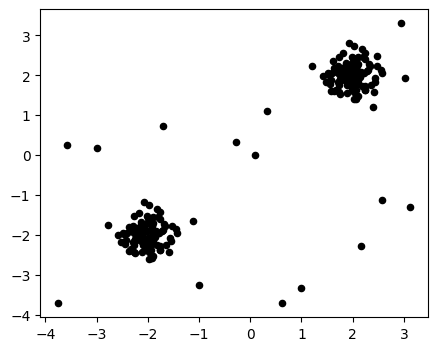
\includegraphics{빅데이터1_files/figure-pdf/cell-22-output-1.png}

\begin{Shaded}
\begin{Highlighting}[]
\ImportTok{from}\NormalTok{ sklearn.neighbors }\ImportTok{import}\NormalTok{ LocalOutlierFactor}
\NormalTok{clf }\OperatorTok{=}\NormalTok{ LocalOutlierFactor(n\_neighbors}\OperatorTok{=}\DecValTok{20}\NormalTok{, contamination}\OperatorTok{=}\FloatTok{0.1}\NormalTok{)}
\NormalTok{y\_pred }\OperatorTok{=}\NormalTok{ clf.fit\_predict(X) }\CommentTok{\# 1: inlier, {-}1: outlier}
\NormalTok{outlier\_mask }\OperatorTok{=}\NormalTok{ y\_pred }\OperatorTok{==} \OperatorTok{{-}}\DecValTok{1}

\NormalTok{plt.figure(figsize}\OperatorTok{=}\NormalTok{(}\DecValTok{5}\NormalTok{, }\DecValTok{4}\NormalTok{))}
\NormalTok{plt.scatter(X[:, }\DecValTok{0}\NormalTok{], X[:, }\DecValTok{1}\NormalTok{], color}\OperatorTok{=}\StringTok{\textquotesingle{}b\textquotesingle{}}\NormalTok{, s}\OperatorTok{=}\DecValTok{20}\NormalTok{, label}\OperatorTok{=}\StringTok{\textquotesingle{}Inliers\textquotesingle{}}\NormalTok{)}
\NormalTok{plt.scatter(X[outlier\_mask, }\DecValTok{0}\NormalTok{], X[outlier\_mask, }\DecValTok{1}\NormalTok{], color}\OperatorTok{=}\StringTok{\textquotesingle{}r\textquotesingle{}}\NormalTok{, s}\OperatorTok{=}\DecValTok{50}\NormalTok{,label}\OperatorTok{=}\StringTok{\textquotesingle{}Outliers\textquotesingle{}}\NormalTok{)}
\NormalTok{plt.xlabel(}\StringTok{"Feature 1"}\NormalTok{)}
\NormalTok{plt.ylabel(}\StringTok{"Feature 2"}\NormalTok{)}
\NormalTok{plt.legend()}
\end{Highlighting}
\end{Shaded}

\includegraphics{빅데이터1_files/figure-pdf/cell-23-output-1.png}

\begin{Shaded}
\begin{Highlighting}[]
\ImportTok{from}\NormalTok{ sklearn.ensemble }\ImportTok{import}\NormalTok{ IsolationForest}
\NormalTok{clf2 }\OperatorTok{=}\NormalTok{ IsolationForest(contamination}\OperatorTok{=}\FloatTok{0.1}\NormalTok{)}
\CommentTok{\# contamination : 이상치 비율}
\CommentTok{\# n\_estimators : 나무의 갯수 (defalut 100)}
\CommentTok{\# max\_features : 각 나무별 특성변수의 갯수(default 1)}
\NormalTok{clf2.fit( X )}
\NormalTok{y\_pred2 }\OperatorTok{=}\NormalTok{ clf2.predict( X ) }\CommentTok{\# 1: inlier, {-}1: outlier}
\NormalTok{outlier\_mask2 }\OperatorTok{=}\NormalTok{ y\_pred2 }\OperatorTok{==} \OperatorTok{{-}}\DecValTok{1}

\NormalTok{plt.figure(figsize}\OperatorTok{=}\NormalTok{(}\DecValTok{5}\NormalTok{, }\DecValTok{4}\NormalTok{))}
\NormalTok{plt.scatter(X[:, }\DecValTok{0}\NormalTok{], X[:, }\DecValTok{1}\NormalTok{], color}\OperatorTok{=}\StringTok{\textquotesingle{}b\textquotesingle{}}\NormalTok{, s}\OperatorTok{=}\DecValTok{20}\NormalTok{, label}\OperatorTok{=}\StringTok{\textquotesingle{}Inliers\textquotesingle{}}\NormalTok{)}
\NormalTok{plt.scatter(X[outlier\_mask2, }\DecValTok{0}\NormalTok{], X[outlier\_mask2, }\DecValTok{1}\NormalTok{], color}\OperatorTok{=}\StringTok{\textquotesingle{}r\textquotesingle{}}\NormalTok{, s}\OperatorTok{=}\DecValTok{50}\NormalTok{,label}\OperatorTok{=}\StringTok{\textquotesingle{}Outliers\textquotesingle{}}\NormalTok{)}
\NormalTok{plt.xlabel(}\StringTok{"Feature 1"}\NormalTok{)}
\NormalTok{plt.ylabel(}\StringTok{"Feature 2"}\NormalTok{)}
\NormalTok{plt.legend()}
\end{Highlighting}
\end{Shaded}

\includegraphics{빅데이터1_files/figure-pdf/cell-24-output-1.png}

\begin{Shaded}
\begin{Highlighting}[]
\NormalTok{clf2.score\_samples(X)}
\end{Highlighting}
\end{Shaded}

\begin{verbatim}
array([-0.39567479, -0.43973362, -0.38576701, -0.4625295 , -0.39169087,
       -0.39353101, -0.44632054, -0.4539587 , -0.39410011, -0.42823486,
       -0.43802322, -0.4231585 , -0.38600184, -0.40324911, -0.38778406,
       -0.46849881, -0.4075734 , -0.43420431, -0.45140279, -0.4113938 ,
       -0.40036102, -0.38335266, -0.42666089, -0.41104579, -0.44476313,
       -0.38744281, -0.39942914, -0.44257912, -0.38938554, -0.40470075,
       -0.39006555, -0.42881353, -0.44275864, -0.40154039, -0.39729665,
       -0.42434279, -0.42743206, -0.57699503, -0.38628797, -0.45454533,
       -0.3864026 , -0.44513991, -0.39598029, -0.41231495, -0.39270763,
       -0.40568073, -0.39005843, -0.43210962, -0.38601781, -0.38485125,
       -0.41991455, -0.40181793, -0.38788591, -0.48400217, -0.38538727,
       -0.47693547, -0.50815903, -0.39115267, -0.40423505, -0.43216634,
       -0.4254748 , -0.48475901, -0.4890737 , -0.40357175, -0.39439224,
       -0.42406868, -0.40171635, -0.44870204, -0.38761922, -0.43170548,
       -0.42364173, -0.43593615, -0.39560581, -0.4391784 , -0.39543452,
       -0.38550106, -0.38910014, -0.39558501, -0.48693408, -0.41865632,
       -0.40964165, -0.43730378, -0.41716448, -0.47893783, -0.39791987,
       -0.40492088, -0.38431516, -0.39544321, -0.42208103, -0.53522817,
       -0.41839783, -0.40171635, -0.39362168, -0.39333773, -0.44128807,
       -0.40208128, -0.40907841, -0.39096216, -0.38929625, -0.40645206,
       -0.38953796, -0.43147334, -0.38691831, -0.45292849, -0.39365031,
       -0.40064735, -0.46513506, -0.48209563, -0.39635657, -0.44569517,
       -0.4496465 , -0.43243444, -0.39406682, -0.40625773, -0.39826724,
       -0.46462545, -0.40782229, -0.42572527, -0.46599338, -0.42852596,
       -0.40082304, -0.38971614, -0.4628486 , -0.4219109 , -0.46365237,
       -0.39237271, -0.40320941, -0.42432754, -0.40309339, -0.40204058,
       -0.39044555, -0.43501511, -0.4324525 , -0.40503508, -0.40259674,
       -0.42956023, -0.42799201, -0.56257644, -0.38875652, -0.47585014,
       -0.3835507 , -0.4556408 , -0.406217  , -0.40385118, -0.39458774,
       -0.40122018, -0.40401747, -0.4443972 , -0.38320086, -0.3834212 ,
       -0.44945534, -0.4060406 , -0.38476589, -0.46817324, -0.38466101,
       -0.47610349, -0.49275615, -0.38344594, -0.40974845, -0.42395885,
       -0.42189161, -0.49261883, -0.48518689, -0.40901991, -0.39452123,
       -0.44785724, -0.40375287, -0.45749968, -0.40496115, -0.4260838 ,
       -0.41810669, -0.44560803, -0.38806155, -0.45523273, -0.38817405,
       -0.38177641, -0.39724261, -0.40279204, -0.46677259, -0.42162856,
       -0.4086809 , -0.43961327, -0.40404401, -0.45862325, -0.40473907,
       -0.41509113, -0.38081908, -0.39036169, -0.42441162, -0.52130968,
       -0.41557892, -0.40347146, -0.39318444, -0.38921027, -0.46342999,
       -0.39756969, -0.41357841, -0.38429305, -0.40297782, -0.40881293,
       -0.60259641, -0.44411547, -0.57052254, -0.50247903, -0.73212838,
       -0.64786135, -0.55623141, -0.45375541, -0.68754218, -0.67833274,
       -0.70698798, -0.63422967, -0.64031155, -0.78183101, -0.65477657,
       -0.67178443, -0.67084008, -0.68580391, -0.71446705, -0.64861428])
\end{verbatim}

\chapter{빅데이터와 금융자료 분석
기말대체과제}\label{uxbe45uxb370uxc774uxd130uxc640-uxae08uxc735uxc790uxb8cc-uxbd84uxc11d-uxae30uxb9d0uxb300uxccb4uxacfcuxc81c}

20249132 김형환

\section{Question 1}\label{question-1}

\begin{center}
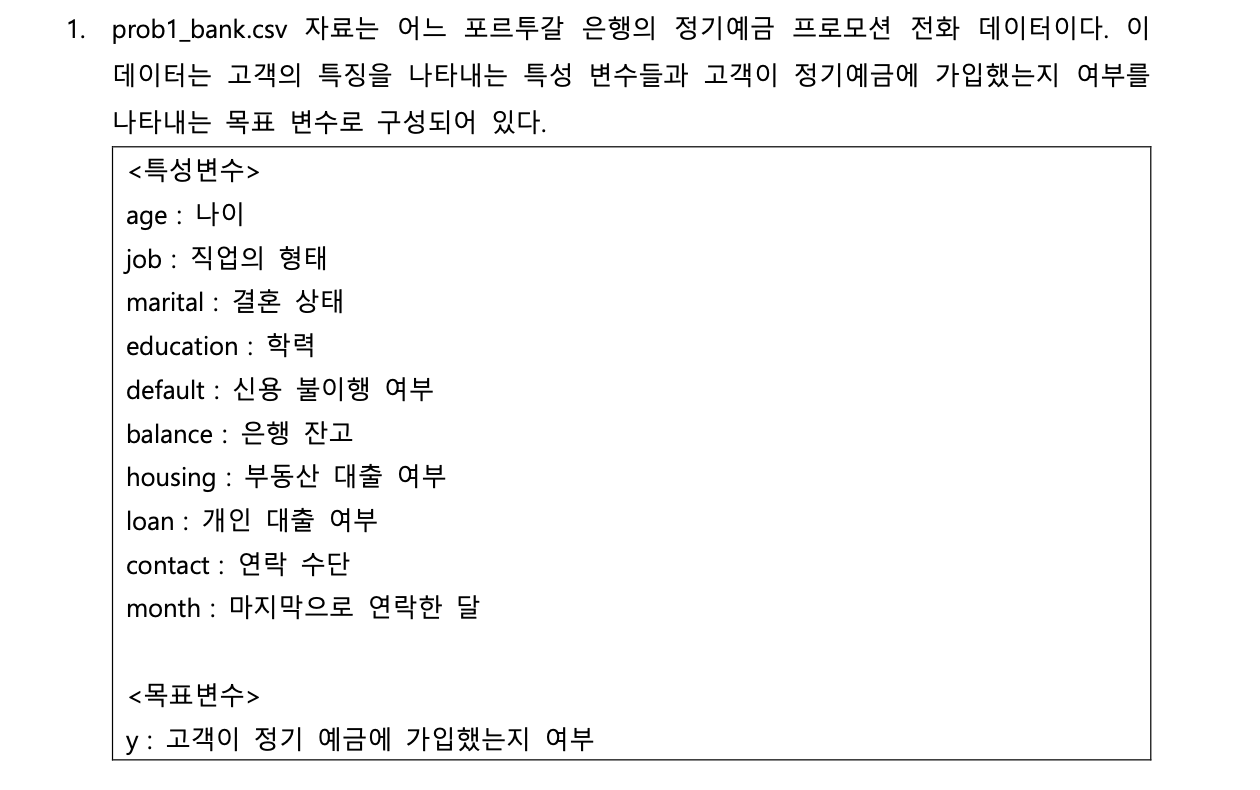
\includegraphics[width=0.7\textwidth,height=\textheight]{image/bigdata1.png}
\end{center}

\subsection{(1)}\label{section}

주어진 자료 중 범주형 변수 각각에 대해 적절한 전처리를 선택하고
진행하여라.

\begin{Shaded}
\begin{Highlighting}[]
\ImportTok{import}\NormalTok{ numpy }\ImportTok{as}\NormalTok{ np}
\ImportTok{import}\NormalTok{ pandas }\ImportTok{as}\NormalTok{ pd}

\NormalTok{bank }\OperatorTok{=}\NormalTok{ pd.read\_csv(}\StringTok{\textquotesingle{}data/prob1\_bank.csv\textquotesingle{}}\NormalTok{)}
\NormalTok{bank.info() }\CommentTok{\# 전체 11개 칼럼에 null값은 없으며, 범주형 9개 및 숫자형 2개}
\end{Highlighting}
\end{Shaded}

\begin{verbatim}
<class 'pandas.core.frame.DataFrame'>
RangeIndex: 4521 entries, 0 to 4520
Data columns (total 11 columns):
 #   Column     Non-Null Count  Dtype 
---  ------     --------------  ----- 
 0   age        4521 non-null   int64 
 1   job        4521 non-null   object
 2   marital    4521 non-null   object
 3   education  4521 non-null   object
 4   default    4521 non-null   object
 5   balance    4521 non-null   int64 
 6   housing    4521 non-null   object
 7   loan       4521 non-null   object
 8   contact    4521 non-null   object
 9   month      4521 non-null   object
 10  y          4521 non-null   object
dtypes: int64(2), object(9)
memory usage: 388.6+ KB
\end{verbatim}

\begin{Shaded}
\begin{Highlighting}[]
\NormalTok{bank.select\_dtypes(include}\OperatorTok{=}\StringTok{\textquotesingle{}object\textquotesingle{}}\NormalTok{).nunique()}
\CommentTok{\# 범주형 9개 중, 목적변수를 포함하여 4개는 \textquotesingle{}여부\textquotesingle{}에 대한 이진변수이며 나머지는 3\textasciitilde{}12개의 고유값}
\end{Highlighting}
\end{Shaded}

\begin{verbatim}
job          12
marital       3
education     4
default       2
housing       2
loan          2
contact       3
month        12
y             2
dtype: int64
\end{verbatim}

\begin{Shaded}
\begin{Highlighting}[]
\NormalTok{bank[}\StringTok{\textquotesingle{}job\textquotesingle{}}\NormalTok{].value\_counts()}
\CommentTok{\# 직업의 경우, 12개의 범주로 구성됨. 특별히 한 값에 치중되는 모습도 보이지 않고,}
\CommentTok{\# 순서가 없으므로 원{-}핫 인코딩으로 처리 예정}
\end{Highlighting}
\end{Shaded}

\begin{verbatim}
job
management       969
blue-collar      946
technician       768
admin.           478
services         417
retired          230
self-employed    183
entrepreneur     168
unemployed       128
housemaid        112
student           84
unknown           38
Name: count, dtype: int64
\end{verbatim}

\begin{Shaded}
\begin{Highlighting}[]
\NormalTok{bank[}\StringTok{\textquotesingle{}marital\textquotesingle{}}\NormalTok{].value\_counts()}
\CommentTok{\# 결혼 여부는 싱글/결혼/이혼 3진변수임. 순서가 없으므로 원{-}핫 인코딩으로 처리 예정}
\end{Highlighting}
\end{Shaded}

\begin{verbatim}
marital
married     2797
single      1196
divorced     528
Name: count, dtype: int64
\end{verbatim}

\begin{Shaded}
\begin{Highlighting}[]
\NormalTok{bank[}\StringTok{\textquotesingle{}education\textquotesingle{}}\NormalTok{].value\_counts()}
\CommentTok{\# 학력에 대한 내용은 primary {-} secondary {-} tertiary 순이므로 1\textasciitilde{}3 라벨인코딩 처리 예정}
\CommentTok{\# unknown은 학력수준이 낮을 가능성이 높을 것으로 추정, 0으로 처리하여 하나의 응답값으로 간주함.}
\end{Highlighting}
\end{Shaded}

\begin{verbatim}
education
secondary    2306
tertiary     1350
primary       678
unknown       187
Name: count, dtype: int64
\end{verbatim}

\begin{Shaded}
\begin{Highlighting}[]
\NormalTok{bank[}\StringTok{\textquotesingle{}contact\textquotesingle{}}\NormalTok{].value\_counts()}
\CommentTok{\# 연락방법에 대한 내용은 telephone {-} cellular 순으로 연락이 편리하므로 1\textasciitilde{}2 라벨인코딩 처리 예정}
\CommentTok{\# unknown은 연락 편의성이 가장 떨어질 것으로 보임. 0으로 처리하여 라벨인코딩 처리 예정}
\end{Highlighting}
\end{Shaded}

\begin{verbatim}
contact
cellular     2896
unknown      1324
telephone     301
Name: count, dtype: int64
\end{verbatim}

\begin{Shaded}
\begin{Highlighting}[]
\NormalTok{bank[}\StringTok{\textquotesingle{}month\textquotesingle{}}\NormalTok{].value\_counts()}
\CommentTok{\# 달에 대한 내용으로, 1\textasciitilde{}12개월 순서에 따른 라벨인코딩 처리 예정}
\end{Highlighting}
\end{Shaded}

\begin{verbatim}
month
may    1398
jul     706
aug     633
jun     531
nov     389
apr     293
feb     222
jan     148
oct      80
sep      52
mar      49
dec      20
Name: count, dtype: int64
\end{verbatim}

\begin{Shaded}
\begin{Highlighting}[]
\CommentTok{\# 범주형 변수 처리}

\CommentTok{\# 1. job, marital {-}\textgreater{} One{-}Hot Encoding}
\NormalTok{bank }\OperatorTok{=}\NormalTok{ pd.get\_dummies(bank, columns}\OperatorTok{=}\NormalTok{[}\StringTok{\textquotesingle{}job\textquotesingle{}}\NormalTok{, }\StringTok{\textquotesingle{}marital\textquotesingle{}}\NormalTok{], drop\_first}\OperatorTok{=}\VariableTok{True}\NormalTok{)}

\CommentTok{\# 2. education, contact, month \textgreater{} Label Encoding}
\NormalTok{edu\_map }\OperatorTok{=}\NormalTok{ \{}\StringTok{\textquotesingle{}unknown\textquotesingle{}}\NormalTok{: }\DecValTok{0}\NormalTok{,}\StringTok{\textquotesingle{}primary\textquotesingle{}}\NormalTok{: }\DecValTok{1}\NormalTok{,}\StringTok{\textquotesingle{}secondary\textquotesingle{}}\NormalTok{: }\DecValTok{2}\NormalTok{,}\StringTok{\textquotesingle{}tertiary\textquotesingle{}}\NormalTok{: }\DecValTok{3}\NormalTok{\}}
\NormalTok{bank[}\StringTok{\textquotesingle{}education\textquotesingle{}}\NormalTok{] }\OperatorTok{=}\NormalTok{ bank[}\StringTok{\textquotesingle{}education\textquotesingle{}}\NormalTok{].}\BuiltInTok{map}\NormalTok{(edu\_map)}

\NormalTok{contact\_map }\OperatorTok{=}\NormalTok{ \{}\StringTok{\textquotesingle{}unknown\textquotesingle{}}\NormalTok{: }\DecValTok{0}\NormalTok{,}\StringTok{\textquotesingle{}telephone\textquotesingle{}}\NormalTok{: }\DecValTok{1}\NormalTok{,}\StringTok{\textquotesingle{}cellular\textquotesingle{}}\NormalTok{: }\DecValTok{2}\NormalTok{\}}
\NormalTok{bank[}\StringTok{\textquotesingle{}contact\textquotesingle{}}\NormalTok{] }\OperatorTok{=}\NormalTok{ bank[}\StringTok{\textquotesingle{}contact\textquotesingle{}}\NormalTok{].}\BuiltInTok{map}\NormalTok{(contact\_map)}

\NormalTok{month\_order }\OperatorTok{=}\NormalTok{ [}\StringTok{\textquotesingle{}jan\textquotesingle{}}\NormalTok{, }\StringTok{\textquotesingle{}feb\textquotesingle{}}\NormalTok{, }\StringTok{\textquotesingle{}mar\textquotesingle{}}\NormalTok{, }\StringTok{\textquotesingle{}apr\textquotesingle{}}\NormalTok{, }\StringTok{\textquotesingle{}may\textquotesingle{}}\NormalTok{, }\StringTok{\textquotesingle{}jun\textquotesingle{}}\NormalTok{,}
               \StringTok{\textquotesingle{}jul\textquotesingle{}}\NormalTok{, }\StringTok{\textquotesingle{}aug\textquotesingle{}}\NormalTok{, }\StringTok{\textquotesingle{}sep\textquotesingle{}}\NormalTok{, }\StringTok{\textquotesingle{}oct\textquotesingle{}}\NormalTok{, }\StringTok{\textquotesingle{}nov\textquotesingle{}}\NormalTok{, }\StringTok{\textquotesingle{}dec\textquotesingle{}}\NormalTok{]}
\NormalTok{month\_map }\OperatorTok{=}\NormalTok{ \{month: i }\ControlFlowTok{for}\NormalTok{ i, month }\KeywordTok{in} \BuiltInTok{enumerate}\NormalTok{(month\_order)\}}
\NormalTok{bank[}\StringTok{\textquotesingle{}month\textquotesingle{}}\NormalTok{] }\OperatorTok{=}\NormalTok{ bank[}\StringTok{\textquotesingle{}month\textquotesingle{}}\NormalTok{].}\BuiltInTok{map}\NormalTok{(month\_map)}

\CommentTok{\# 3. default, housing, loan, y \textgreater{} Label Encoding (binary, yes=1 / no=0)}
\NormalTok{binary\_cols }\OperatorTok{=}\NormalTok{ [}\StringTok{\textquotesingle{}default\textquotesingle{}}\NormalTok{, }\StringTok{\textquotesingle{}housing\textquotesingle{}}\NormalTok{, }\StringTok{\textquotesingle{}loan\textquotesingle{}}\NormalTok{, }\StringTok{\textquotesingle{}y\textquotesingle{}}\NormalTok{]}
\ControlFlowTok{for}\NormalTok{ col }\KeywordTok{in}\NormalTok{ binary\_cols: bank[col] }\OperatorTok{=}\NormalTok{ bank[col].}\BuiltInTok{map}\NormalTok{(\{}\StringTok{\textquotesingle{}yes\textquotesingle{}}\NormalTok{: }\DecValTok{1}\NormalTok{, }\StringTok{\textquotesingle{}no\textquotesingle{}}\NormalTok{: }\DecValTok{0}\NormalTok{\})}

\BuiltInTok{print}\NormalTok{(bank.info())}
\end{Highlighting}
\end{Shaded}

\begin{verbatim}
<class 'pandas.core.frame.DataFrame'>
RangeIndex: 4521 entries, 0 to 4520
Data columns (total 22 columns):
 #   Column             Non-Null Count  Dtype
---  ------             --------------  -----
 0   age                4521 non-null   int64
 1   education          4521 non-null   int64
 2   default            4521 non-null   int64
 3   balance            4521 non-null   int64
 4   housing            4521 non-null   int64
 5   loan               4521 non-null   int64
 6   contact            4521 non-null   int64
 7   month              4521 non-null   int64
 8   y                  4521 non-null   int64
 9   job_blue-collar    4521 non-null   bool 
 10  job_entrepreneur   4521 non-null   bool 
 11  job_housemaid      4521 non-null   bool 
 12  job_management     4521 non-null   bool 
 13  job_retired        4521 non-null   bool 
 14  job_self-employed  4521 non-null   bool 
 15  job_services       4521 non-null   bool 
 16  job_student        4521 non-null   bool 
 17  job_technician     4521 non-null   bool 
 18  job_unemployed     4521 non-null   bool 
 19  job_unknown        4521 non-null   bool 
 20  marital_married    4521 non-null   bool 
 21  marital_single     4521 non-null   bool 
dtypes: bool(13), int64(9)
memory usage: 375.4 KB
None
\end{verbatim}

\subsection{(2)}\label{section-1}

주어진 자료 중 수치형 변수 각각에 대해 적절한 전처리를 선택하고
진행하여라.

\begin{Shaded}
\begin{Highlighting}[]
\ImportTok{import}\NormalTok{ matplotlib.pyplot }\ImportTok{as}\NormalTok{ plt}
\ImportTok{import}\NormalTok{ seaborn }\ImportTok{as}\NormalTok{ sns}

\CommentTok{\# 1. age 분포}
\NormalTok{plt.figure(figsize}\OperatorTok{=}\NormalTok{(}\DecValTok{10}\NormalTok{, }\DecValTok{4}\NormalTok{))}
\NormalTok{sns.histplot(bank[}\StringTok{\textquotesingle{}age\textquotesingle{}}\NormalTok{], bins}\OperatorTok{=}\DecValTok{30}\NormalTok{, kde}\OperatorTok{=}\VariableTok{True}\NormalTok{)}
\NormalTok{plt.title(}\StringTok{"Distribution of Age"}\NormalTok{)}
\NormalTok{plt.xlabel(}\StringTok{"Age"}\NormalTok{)}
\NormalTok{plt.ylabel(}\StringTok{"Count"}\NormalTok{)}
\NormalTok{plt.tight\_layout()}
\NormalTok{plt.show()}

\CommentTok{\# 2. balance 분포}
\NormalTok{plt.figure(figsize}\OperatorTok{=}\NormalTok{(}\DecValTok{10}\NormalTok{, }\DecValTok{4}\NormalTok{))}
\NormalTok{sns.histplot(bank[}\StringTok{\textquotesingle{}balance\textquotesingle{}}\NormalTok{], bins}\OperatorTok{=}\DecValTok{30}\NormalTok{, kde}\OperatorTok{=}\VariableTok{True}\NormalTok{)}
\NormalTok{plt.title(}\StringTok{"Distribution of Balance"}\NormalTok{)}
\NormalTok{plt.xlabel(}\StringTok{"Balance"}\NormalTok{)}
\NormalTok{plt.ylabel(}\StringTok{"Count"}\NormalTok{)}
\NormalTok{plt.tight\_layout()}
\NormalTok{plt.show()}
\end{Highlighting}
\end{Shaded}

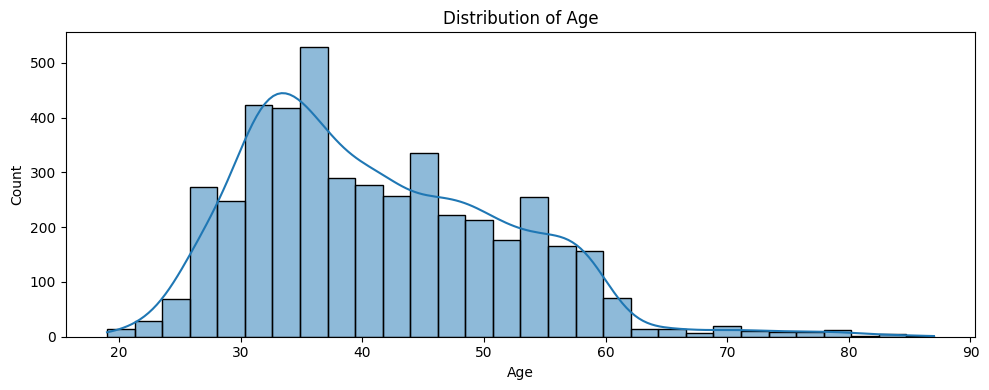
\includegraphics{빅데이터_과제_files/figure-pdf/cell-10-output-1.png}

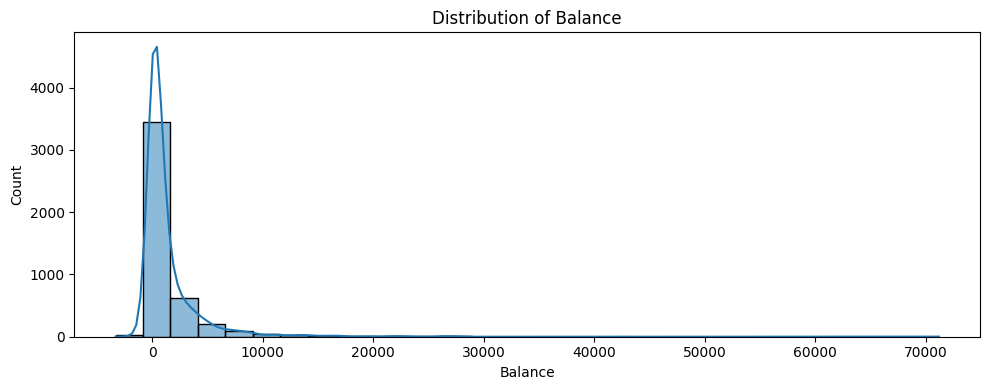
\includegraphics{빅데이터_과제_files/figure-pdf/cell-10-output-2.png}

\begin{Shaded}
\begin{Highlighting}[]
\NormalTok{bank[}\StringTok{\textquotesingle{}age\textquotesingle{}}\NormalTok{].describe()}
\CommentTok{\# age는 오른쪽 skew가 미세하게 있는 정규분포와 가까운 형태. 표준화만 진행}
\end{Highlighting}
\end{Shaded}

\begin{verbatim}
count    4521.000000
mean       41.170095
std        10.576211
min        19.000000
25%        33.000000
50%        39.000000
75%        49.000000
max        87.000000
Name: age, dtype: float64
\end{verbatim}

\begin{Shaded}
\begin{Highlighting}[]
\NormalTok{bank[}\StringTok{\textquotesingle{}balance\textquotesingle{}}\NormalTok{].describe()}
\CommentTok{\# balance는 음수도 존재하고, 값이 매우 극단적으로 치우쳐져 있는 형태. log변환 및 표준화 진행}
\CommentTok{\# 이후 LOF 방식으로 두 수치형변수에 대한 이상치 탐지, 약 1\% 수준의 이상치 제거 예정}
\end{Highlighting}
\end{Shaded}

\begin{verbatim}
count     4521.000000
mean      1422.657819
std       3009.638142
min      -3313.000000
25%         69.000000
50%        444.000000
75%       1480.000000
max      71188.000000
Name: balance, dtype: float64
\end{verbatim}

\begin{Shaded}
\begin{Highlighting}[]
\ImportTok{from}\NormalTok{ sklearn.preprocessing }\ImportTok{import}\NormalTok{ StandardScaler}
\ImportTok{from}\NormalTok{ sklearn.neighbors }\ImportTok{import}\NormalTok{ LocalOutlierFactor}
\ImportTok{import}\NormalTok{ numpy }\ImportTok{as}\NormalTok{ np}

\CommentTok{\# 1. balance 로그변환 (음수 대비)}
\NormalTok{min\_bal }\OperatorTok{=}\NormalTok{ bank[}\StringTok{\textquotesingle{}balance\textquotesingle{}}\NormalTok{].}\BuiltInTok{min}\NormalTok{()}
\NormalTok{bank[}\StringTok{\textquotesingle{}log\_balance\textquotesingle{}}\NormalTok{] }\OperatorTok{=}\NormalTok{ np.log1p(bank[}\StringTok{\textquotesingle{}balance\textquotesingle{}}\NormalTok{] }\OperatorTok{{-}}\NormalTok{ min\_bal }\OperatorTok{+} \DecValTok{1}\NormalTok{)}

\CommentTok{\# 2. balance + age 표준화}
\NormalTok{scaler }\OperatorTok{=}\NormalTok{ StandardScaler()}
\NormalTok{bank[[}\StringTok{\textquotesingle{}std\_log\_balance\textquotesingle{}}\NormalTok{, }\StringTok{\textquotesingle{}std\_age\textquotesingle{}}\NormalTok{]] }\OperatorTok{=}\NormalTok{ scaler.fit\_transform(bank[[}\StringTok{\textquotesingle{}log\_balance\textquotesingle{}}\NormalTok{, }\StringTok{\textquotesingle{}age\textquotesingle{}}\NormalTok{]])}

\CommentTok{\# 3. LOF 이상치 탐지 (다변량: log\_balance + age)}
\CommentTok{\# 적절한 파라미터 조정으로 balance의 최소, 최대값을 효과적으로 제거}
\NormalTok{X\_scaled }\OperatorTok{=}\NormalTok{ bank[[}\StringTok{\textquotesingle{}std\_log\_balance\textquotesingle{}}\NormalTok{, }\StringTok{\textquotesingle{}std\_age\textquotesingle{}}\NormalTok{]]}
\NormalTok{lof }\OperatorTok{=}\NormalTok{ LocalOutlierFactor(n\_neighbors}\OperatorTok{=}\DecValTok{30}\NormalTok{, contamination}\OperatorTok{=}\FloatTok{0.01}\NormalTok{)}
\NormalTok{bank[}\StringTok{\textquotesingle{}is\_outlier\textquotesingle{}}\NormalTok{] }\OperatorTok{=}\NormalTok{ (lof.fit\_predict(X\_scaled) }\OperatorTok{==} \OperatorTok{{-}}\DecValTok{1}\NormalTok{).astype(}\BuiltInTok{int}\NormalTok{)}

\CommentTok{\# 4. 이상치 시각화 (scatter plot)}
\NormalTok{plt.figure(figsize}\OperatorTok{=}\NormalTok{(}\DecValTok{10}\NormalTok{, }\DecValTok{6}\NormalTok{))}
\NormalTok{sns.scatterplot(data}\OperatorTok{=}\NormalTok{bank, x}\OperatorTok{=}\StringTok{\textquotesingle{}std\_log\_balance\textquotesingle{}}\NormalTok{, y}\OperatorTok{=}\StringTok{\textquotesingle{}std\_age\textquotesingle{}}\NormalTok{,}
\NormalTok{                hue}\OperatorTok{=}\StringTok{\textquotesingle{}is\_outlier\textquotesingle{}}\NormalTok{, palette}\OperatorTok{=}\StringTok{\textquotesingle{}Set1\textquotesingle{}}\NormalTok{, alpha}\OperatorTok{=}\FloatTok{0.7}\NormalTok{)}
\NormalTok{plt.title(}\StringTok{"Scatter Plot of Standardized Log Balance vs. Age}\CharTok{\textbackslash{}n}\StringTok{(LOF Outlier Detection)"}\NormalTok{)}
\NormalTok{plt.xlabel(}\StringTok{"Standardized Log Balance"}\NormalTok{)}
\NormalTok{plt.ylabel(}\StringTok{"Standardized Age"}\NormalTok{)}
\NormalTok{plt.legend(title}\OperatorTok{=}\StringTok{"Outlier"}\NormalTok{)}
\NormalTok{plt.tight\_layout()}
\NormalTok{plt.show()}
\end{Highlighting}
\end{Shaded}

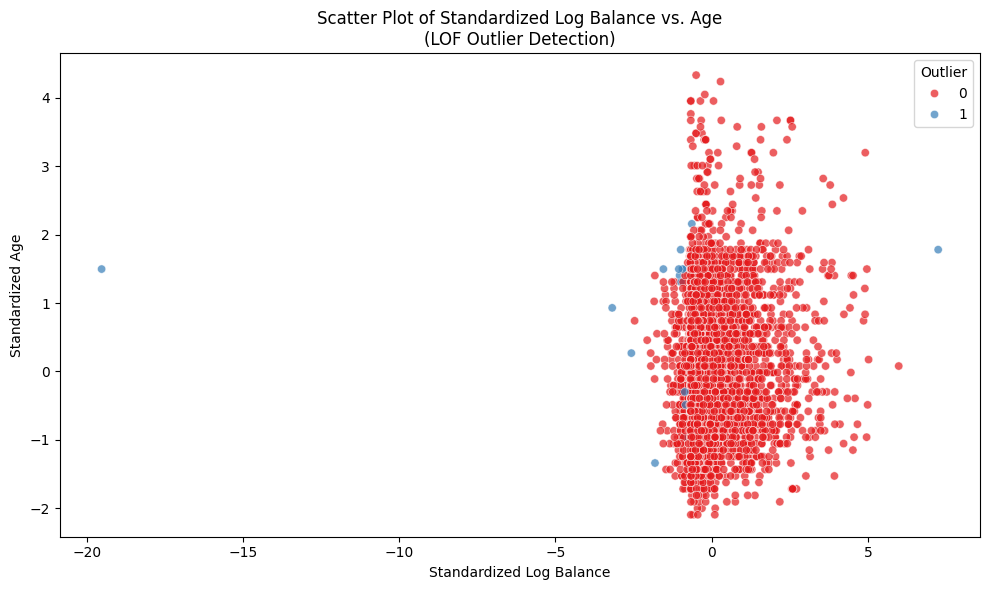
\includegraphics{빅데이터_과제_files/figure-pdf/cell-13-output-1.png}

\begin{Shaded}
\begin{Highlighting}[]
\CommentTok{\# 이상치 1\%가 제거된 것을 확인할 수 있음}
\NormalTok{bank\_clean }\OperatorTok{=}\NormalTok{ bank[bank[}\StringTok{\textquotesingle{}is\_outlier\textquotesingle{}}\NormalTok{] }\OperatorTok{==} \DecValTok{0}\NormalTok{].copy()}
\NormalTok{bank\_clean}
\end{Highlighting}
\end{Shaded}

\begin{longtable}[]{@{}llllllllllllllllllllll@{}}
\toprule\noalign{}
& age & education & default & balance & housing & loan & contact & month
& y & job\_blue-collar & ... & job\_student & job\_technician &
job\_unemployed & job\_unknown & marital\_married & marital\_single &
log\_balance & std\_log\_balance & std\_age & is\_outlier \\
\midrule\noalign{}
\endhead
\bottomrule\noalign{}
\endlastfoot
0 & 30 & 1 & 0 & 1787 & 0 & 0 & 2 & 9 & 0 & False & ... & False & False
& True & False & True & False & 8.537388 & 0.431049 & -1.056270 & 0 \\
1 & 33 & 2 & 0 & 4789 & 1 & 1 & 2 & 4 & 0 & False & ... & False & False
& False & False & True & False & 9.000113 & 1.608188 & -0.772583 & 0 \\
2 & 35 & 3 & 0 & 1350 & 1 & 0 & 2 & 3 & 0 & False & ... & False & False
& False & False & False & True & 8.447843 & 0.203253 & -0.583458 & 0 \\
3 & 30 & 3 & 0 & 1476 & 1 & 1 & 0 & 5 & 0 & False & ... & False & False
& False & False & True & False & 8.474494 & 0.271052 & -1.056270 & 0 \\
4 & 59 & 2 & 0 & 0 & 1 & 0 & 0 & 4 & 0 & True & ... & False & False &
False & False & True & False & 8.106213 & -0.665829 & 1.686036 & 0 \\
... & ... & ... & ... & ... & ... & ... & ... & ... & ... & ... & ... &
... & ... & ... & ... & ... & ... & ... & ... & ... & ... \\
4515 & 32 & 2 & 0 & 473 & 1 & 0 & 2 & 6 & 0 & False & ... & False &
False & False & False & False & True & 8.239593 & -0.326519 & -0.867145
& 0 \\
4516 & 33 & 2 & 0 & -333 & 1 & 0 & 2 & 6 & 0 & False & ... & False &
False & False & False & True & False & 8.000349 & -0.935138 & -0.772583
& 0 \\
4518 & 57 & 2 & 0 & 295 & 0 & 0 & 2 & 7 & 0 & False & ... & False & True
& False & False & True & False & 8.191463 & -0.448959 & 1.496912 & 0 \\
4519 & 28 & 2 & 0 & 1137 & 0 & 0 & 2 & 1 & 0 & True & ... & False &
False & False & False & True & False & 8.401109 & 0.084364 & -1.245394 &
0 \\
4520 & 44 & 3 & 0 & 1136 & 1 & 1 & 2 & 3 & 0 & False & ... & False &
False & False & False & False & True & 8.400884 & 0.083793 & 0.267602 &
0 \\
\end{longtable}

\subsection{(3)}\label{section-2}

주어진 자료에 클래스 불균형이 있는지 확인한 뒤, 이에 대한 적절한 전처리
방법을 선택하여 진행하여라.

\begin{Shaded}
\begin{Highlighting}[]
\CommentTok{\# 약 9:1로 0(No)의 비율이 압도적으로 많음. 클래스불균형 존재}

\NormalTok{class\_counts }\OperatorTok{=}\NormalTok{ bank\_clean[}\StringTok{\textquotesingle{}y\textquotesingle{}}\NormalTok{].value\_counts(normalize}\OperatorTok{=}\VariableTok{True}\NormalTok{)}
\NormalTok{plt.figure(figsize}\OperatorTok{=}\NormalTok{(}\DecValTok{6}\NormalTok{, }\DecValTok{4}\NormalTok{))}
\NormalTok{sns.barplot(x}\OperatorTok{=}\NormalTok{class\_counts.index, y}\OperatorTok{=}\NormalTok{class\_counts.values, legend}\OperatorTok{=}\VariableTok{False}\NormalTok{)}
\NormalTok{plt.title(}\StringTok{"Class Imbalance"}\NormalTok{)}
\NormalTok{plt.xlabel(}\StringTok{"y"}\NormalTok{)}
\NormalTok{plt.ylim(}\DecValTok{0}\NormalTok{, }\DecValTok{1}\NormalTok{)}
\NormalTok{plt.tight\_layout()}
\NormalTok{plt.show()}
\end{Highlighting}
\end{Shaded}

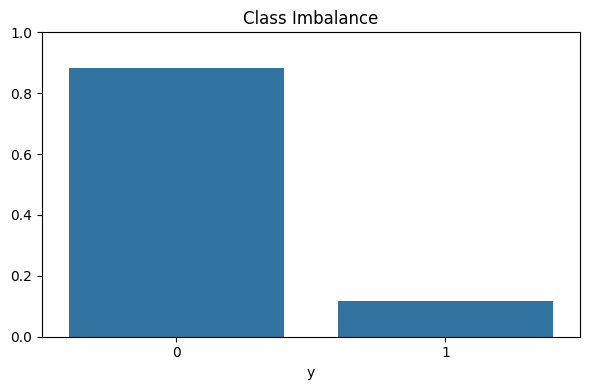
\includegraphics{빅데이터_과제_files/figure-pdf/cell-15-output-1.png}

\begin{Shaded}
\begin{Highlighting}[]
\CommentTok{\# 수치형 변수의 scatter plot상으로 특정 수치형 변수에 따른 치우침은 관측되지 않음.}

\NormalTok{X }\OperatorTok{=}\NormalTok{ bank\_clean[[}\StringTok{\textquotesingle{}std\_log\_balance\textquotesingle{}}\NormalTok{,}\StringTok{\textquotesingle{}std\_age\textquotesingle{}}\NormalTok{]]}
\NormalTok{y }\OperatorTok{=}\NormalTok{ bank\_clean[}\StringTok{\textquotesingle{}y\textquotesingle{}}\NormalTok{]}
\NormalTok{plt.figure(figsize}\OperatorTok{=}\NormalTok{(}\DecValTok{10}\NormalTok{, }\DecValTok{6}\NormalTok{))}
\NormalTok{plt.plot(X.loc[y }\OperatorTok{==} \DecValTok{0}\NormalTok{, }\StringTok{\textquotesingle{}std\_log\_balance\textquotesingle{}}\NormalTok{], X.loc[y }\OperatorTok{==} \DecValTok{0}\NormalTok{, }\StringTok{\textquotesingle{}std\_age\textquotesingle{}}\NormalTok{], }\StringTok{\textquotesingle{}b+\textquotesingle{}}\NormalTok{, label}\OperatorTok{=}\StringTok{"class 0"}\NormalTok{)}
\NormalTok{plt.plot(X.loc[y }\OperatorTok{==} \DecValTok{1}\NormalTok{, }\StringTok{\textquotesingle{}std\_log\_balance\textquotesingle{}}\NormalTok{], X.loc[y }\OperatorTok{==} \DecValTok{1}\NormalTok{, }\StringTok{\textquotesingle{}std\_age\textquotesingle{}}\NormalTok{], }\StringTok{\textquotesingle{}r*\textquotesingle{}}\NormalTok{, label}\OperatorTok{=}\StringTok{"class 1"}\NormalTok{)}
\NormalTok{plt.legend()}
\NormalTok{plt.xlabel(}\StringTok{"std\_log\_balance"}\NormalTok{)}
\NormalTok{plt.ylabel(}\StringTok{"std\_age"}\NormalTok{)}
\NormalTok{plt.title(}\StringTok{"Scatter Plot by Class (y)"}\NormalTok{)}
\NormalTok{plt.show()}
\end{Highlighting}
\end{Shaded}

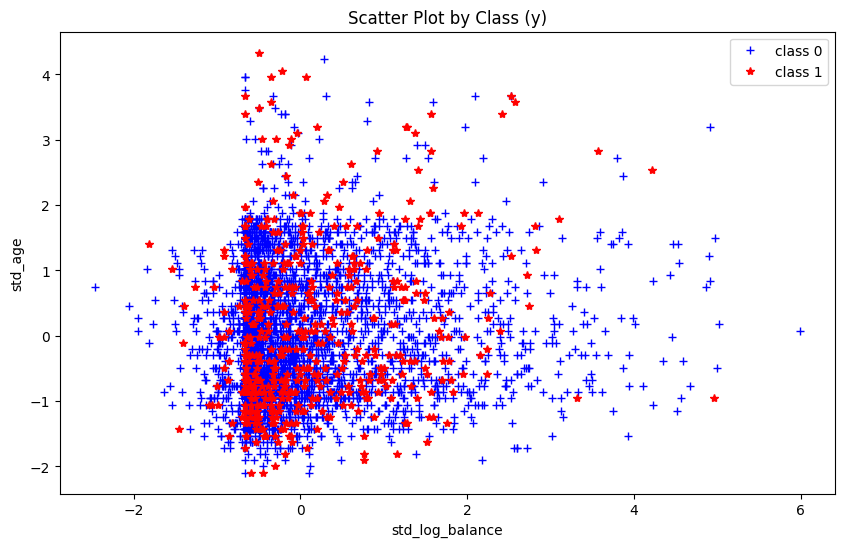
\includegraphics{빅데이터_과제_files/figure-pdf/cell-16-output-1.png}

\begin{Shaded}
\begin{Highlighting}[]
\CommentTok{\# 표본의 수가 적은 편이므로 oversampling 진행}
\CommentTok{\# 데이터의 구조가 그다지 복잡하지 않아 SMOTE 알고리즘을 적용하여 처리}
\ImportTok{from}\NormalTok{ imblearn.over\_sampling }\ImportTok{import}\NormalTok{ SMOTE}

\NormalTok{oversample1 }\OperatorTok{=}\NormalTok{ SMOTE()}
\NormalTok{OX, Oy }\OperatorTok{=}\NormalTok{ oversample1.fit\_resample(X, y)}
\NormalTok{plt.figure(figsize}\OperatorTok{=}\NormalTok{(}\DecValTok{10}\NormalTok{, }\DecValTok{6}\NormalTok{))}
\NormalTok{plt.plot(OX.loc[Oy }\OperatorTok{==} \DecValTok{0}\NormalTok{, }\StringTok{\textquotesingle{}std\_log\_balance\textquotesingle{}}\NormalTok{], OX.loc[Oy }\OperatorTok{==} \DecValTok{0}\NormalTok{, }\StringTok{\textquotesingle{}std\_age\textquotesingle{}}\NormalTok{], }\StringTok{\textquotesingle{}b+\textquotesingle{}}\NormalTok{, label}\OperatorTok{=}\StringTok{"class 0"}\NormalTok{)}
\NormalTok{plt.plot(OX.loc[Oy }\OperatorTok{==} \DecValTok{1}\NormalTok{, }\StringTok{\textquotesingle{}std\_log\_balance\textquotesingle{}}\NormalTok{], OX.loc[Oy }\OperatorTok{==} \DecValTok{1}\NormalTok{, }\StringTok{\textquotesingle{}std\_age\textquotesingle{}}\NormalTok{], }\StringTok{\textquotesingle{}r*\textquotesingle{}}\NormalTok{, label}\OperatorTok{=}\StringTok{"class 1"}\NormalTok{)}
\NormalTok{plt.legend()}
\NormalTok{plt.xlabel(}\StringTok{"std\_log\_balance"}\NormalTok{)}
\NormalTok{plt.ylabel(}\StringTok{"std\_age"}\NormalTok{)}
\NormalTok{plt.title(}\StringTok{"Scatter Plot by Class (y)}\CharTok{\textbackslash{}n}\StringTok{ After Oversampling using SMOTE"}\NormalTok{)}
\NormalTok{plt.show()}
\end{Highlighting}
\end{Shaded}

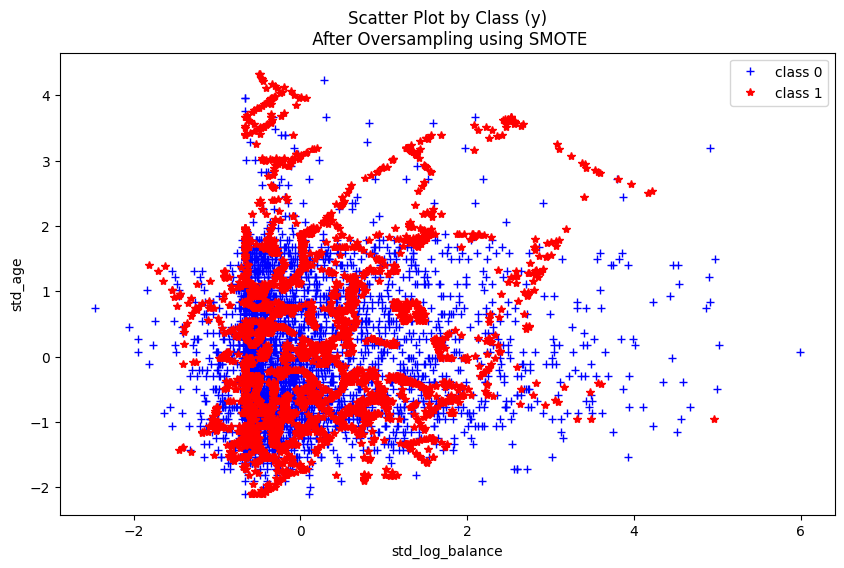
\includegraphics{빅데이터_과제_files/figure-pdf/cell-17-output-1.png}

\section{Question 2}\label{question-2}

\begin{center}
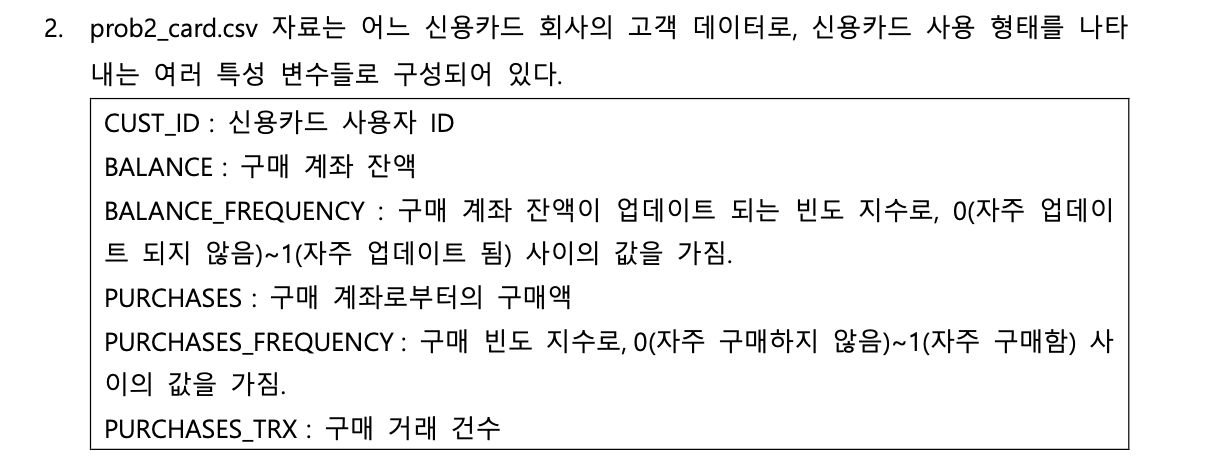
\includegraphics[width=0.7\textwidth,height=\textheight]{image/bigdata2.png}
\end{center}

\subsection{(1)}\label{section-3}

주어진 자료에 K평균 Clustering 알고리즘을 적용하여, 적절한 군집을
생성하여라.

\begin{Shaded}
\begin{Highlighting}[]
\NormalTok{df }\OperatorTok{=}\NormalTok{ pd.read\_csv(}\StringTok{\textquotesingle{}data/prob2\_card.csv\textquotesingle{}}\NormalTok{)}
\NormalTok{df.info()}
\end{Highlighting}
\end{Shaded}

\begin{verbatim}
<class 'pandas.core.frame.DataFrame'>
RangeIndex: 8950 entries, 0 to 8949
Data columns (total 6 columns):
 #   Column               Non-Null Count  Dtype  
---  ------               --------------  -----  
 0   CUST_ID              8950 non-null   object 
 1   BALANCE              8950 non-null   float64
 2   BALANCE_FREQUENCY    8950 non-null   float64
 3   PURCHASES            8950 non-null   float64
 4   PURCHASES_FREQUENCY  8950 non-null   float64
 5   PURCHASES_TRX        8950 non-null   int64  
dtypes: float64(4), int64(1), object(1)
memory usage: 419.7+ KB
\end{verbatim}

\begin{Shaded}
\begin{Highlighting}[]
\NormalTok{df.describe()}
\end{Highlighting}
\end{Shaded}

\begin{longtable}[]{@{}llllll@{}}
\toprule\noalign{}
& BALANCE & BALANCE\_FREQUENCY & PURCHASES & PURCHASES\_FREQUENCY &
PURCHASES\_TRX \\
\midrule\noalign{}
\endhead
\bottomrule\noalign{}
\endlastfoot
count & 8950.000000 & 8950.000000 & 8950.000000 & 8950.000000 &
8950.000000 \\
mean & 1564.474828 & 0.877271 & 1003.204834 & 0.490351 & 14.709832 \\
std & 2081.531879 & 0.236904 & 2136.634782 & 0.401371 & 24.857649 \\
min & 0.000000 & 0.000000 & 0.000000 & 0.000000 & 0.000000 \\
25\% & 128.281915 & 0.888889 & 39.635000 & 0.083333 & 1.000000 \\
50\% & 873.385231 & 1.000000 & 361.280000 & 0.500000 & 7.000000 \\
75\% & 2054.140036 & 1.000000 & 1110.130000 & 0.916667 & 17.000000 \\
max & 19043.138560 & 1.000000 & 49039.570000 & 1.000000 & 358.000000 \\
\end{longtable}

\begin{Shaded}
\begin{Highlighting}[]
\ImportTok{from}\NormalTok{ sklearn.cluster }\ImportTok{import}\NormalTok{ KMeans}
\ImportTok{from}\NormalTok{ sklearn.metrics }\ImportTok{import}\NormalTok{ silhouette\_score}

\CommentTok{\# CUST\_ID는 클러스터링에 사용하지 않으므로 제거}
\NormalTok{X }\OperatorTok{=}\NormalTok{ df.drop(columns}\OperatorTok{=}\NormalTok{[}\StringTok{"CUST\_ID"}\NormalTok{])}

\CommentTok{\# 표준화}
\NormalTok{scaler }\OperatorTok{=}\NormalTok{ StandardScaler()}
\NormalTok{X\_scaled }\OperatorTok{=}\NormalTok{ scaler.fit\_transform(X)}
\NormalTok{scaled\_df }\OperatorTok{=}\NormalTok{ pd.DataFrame(X\_scaled, columns}\OperatorTok{=}\NormalTok{X.columns)}

\CommentTok{\# 최적 K 탐색}
\NormalTok{inertia\_list }\OperatorTok{=}\NormalTok{ []}
\NormalTok{silhouette\_list }\OperatorTok{=}\NormalTok{ []}
\NormalTok{K\_range }\OperatorTok{=} \BuiltInTok{range}\NormalTok{(}\DecValTok{2}\NormalTok{, }\DecValTok{11}\NormalTok{)}

\ControlFlowTok{for}\NormalTok{ k }\KeywordTok{in}\NormalTok{ K\_range:}
\NormalTok{    kmeans }\OperatorTok{=}\NormalTok{ KMeans(n\_clusters}\OperatorTok{=}\NormalTok{k, random\_state}\OperatorTok{=}\DecValTok{42}\NormalTok{, n\_init}\OperatorTok{=}\DecValTok{10}\NormalTok{)}
\NormalTok{    labels }\OperatorTok{=}\NormalTok{ kmeans.fit\_predict(X\_scaled)}
\NormalTok{    inertia\_list.append(kmeans.inertia\_)}
\NormalTok{    silhouette\_list.append(silhouette\_score(X\_scaled, labels))}

\NormalTok{best\_k }\OperatorTok{=}\NormalTok{ K\_range[silhouette\_list.index(}\BuiltInTok{max}\NormalTok{(silhouette\_list))]}

\CommentTok{\# K평균 군집화 결과 : 6개의 군집으로 분류되었으며, 갯수는 32개\textasciitilde{}3200개로 천차만별}
\NormalTok{kmeans\_final }\OperatorTok{=}\NormalTok{ KMeans(n\_clusters}\OperatorTok{=}\NormalTok{best\_k, random\_state}\OperatorTok{=}\DecValTok{42}\NormalTok{, n\_init}\OperatorTok{=}\DecValTok{10}\NormalTok{)}
\NormalTok{scaled\_df[}\StringTok{"KMeans\_Label"}\NormalTok{] }\OperatorTok{=}\NormalTok{ kmeans\_final.fit\_predict(X\_scaled)}

\NormalTok{summary\_table\_kmean }\OperatorTok{=}\NormalTok{ scaled\_df.groupby(}\StringTok{"KMeans\_Label"}\NormalTok{).mean()}
\NormalTok{summary\_table\_kmean[}\StringTok{"Count"}\NormalTok{] }\OperatorTok{=}\NormalTok{ scaled\_df.groupby(}\StringTok{"KMeans\_Label"}\NormalTok{).size()}
\NormalTok{summary\_table\_kmean}
\end{Highlighting}
\end{Shaded}

\begin{longtable}[]{@{}lllllll@{}}
\toprule\noalign{}
& BALANCE & BALANCE\_FREQUENCY & PURCHASES & PURCHASES\_FREQUENCY &
PURCHASES\_TRX & Count \\
KMeans\_Label & & & & & & \\
\midrule\noalign{}
\endhead
\bottomrule\noalign{}
\endlastfoot
0 & -0.679901 & -2.105347 & -0.305189 & -0.528487 & -0.414547 & 1390 \\
1 & 1.906921 & 0.444930 & 10.782703 & 1.119309 & 5.892989 & 32 \\
2 & -0.331950 & 0.368356 & 0.087095 & 0.960328 & 0.227857 & 3253 \\
3 & -0.068576 & 0.366930 & -0.369541 & -0.895659 & -0.502261 & 2989 \\
4 & 0.696282 & 0.475045 & 2.042474 & 1.179006 & 2.713984 & 502 \\
5 & 2.320551 & 0.483046 & -0.159336 & -0.433551 & -0.273897 & 784 \\
\end{longtable}

\begin{Shaded}
\begin{Highlighting}[]
\CommentTok{\# K평균 군집화 시각화}
\NormalTok{summary\_table\_kmean.drop(columns}\OperatorTok{=}\StringTok{"Count"}\NormalTok{).plot.bar(figsize}\OperatorTok{=}\NormalTok{(}\DecValTok{12}\NormalTok{, }\DecValTok{6}\NormalTok{))}
\NormalTok{plt.title(}\StringTok{"Standardized Mean of Variables by KMeans Cluster"}\NormalTok{)}
\NormalTok{plt.xlabel(}\StringTok{"Cluster Label"}\NormalTok{)}
\NormalTok{plt.ylabel(}\StringTok{"Standardized Mean Value"}\NormalTok{)}
\NormalTok{plt.tight\_layout()}
\end{Highlighting}
\end{Shaded}

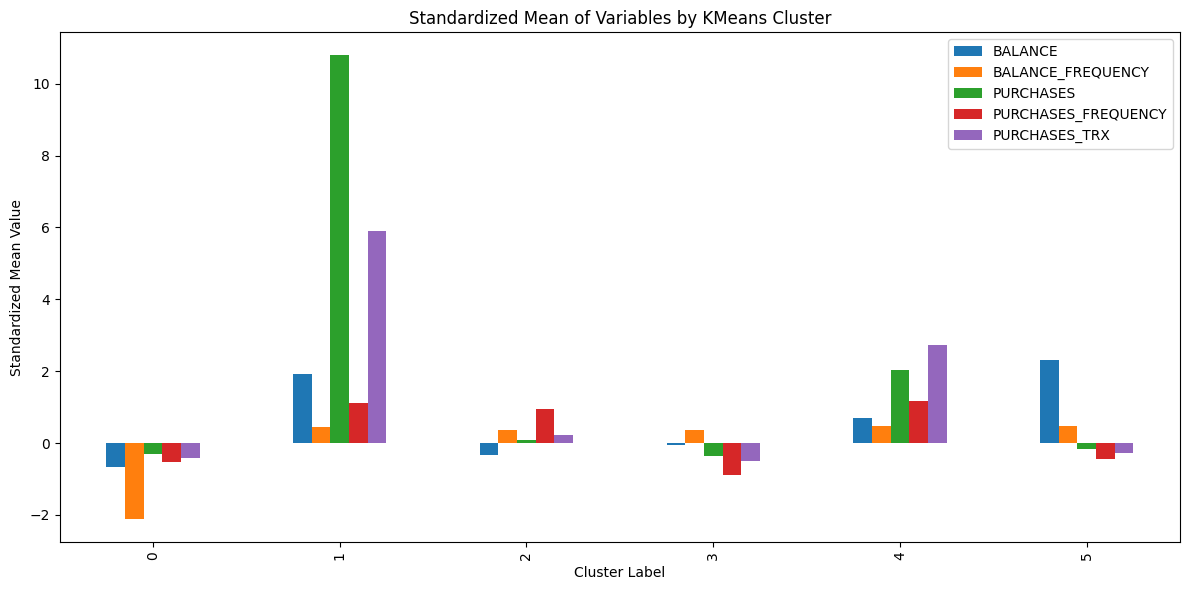
\includegraphics{빅데이터_과제_files/figure-pdf/cell-21-output-1.png}

\subsection{(2)}\label{section-4}

주어진 자료에 DBSCAN Clustering 알고리즘을 적용하여, 적절한 군집을
생성하여라.

\begin{Shaded}
\begin{Highlighting}[]
\ImportTok{from}\NormalTok{ sklearn.cluster }\ImportTok{import}\NormalTok{ DBSCAN}

\CommentTok{\# DBSCAN 분류 : eps 및 min\_samples는 여러번 반복을 통해 최적의 조합을 도출하였음.}
\CommentTok{\# 기준 : 분류가 너무 많거나 적지 않도록(3\textasciitilde{}6개), 너무 숫자가 적은 분류가 없도록}
\NormalTok{dbscan }\OperatorTok{=}\NormalTok{ DBSCAN(eps}\OperatorTok{=}\FloatTok{0.6}\NormalTok{, min\_samples}\OperatorTok{=}\DecValTok{4}\NormalTok{)}
\NormalTok{labels }\OperatorTok{=}\NormalTok{ dbscan.fit\_predict(X\_scaled)}

\CommentTok{\# 라벨을 데이터프레임에 추가}
\NormalTok{scaled\_df[}\StringTok{"DBSCAN\_Label"}\NormalTok{] }\OperatorTok{=}\NormalTok{ labels}

\CommentTok{\# DBSCAN 군집화 결과 : 잡음({-}1)이 약 2\% 포함되어있으며, 총 5개의 군집으로 분류(177개\textasciitilde{}6200개)}
\NormalTok{summary\_table\_db }\OperatorTok{=}\NormalTok{ scaled\_df.drop(columns}\OperatorTok{=}\StringTok{"KMeans\_Label"}\NormalTok{).groupby(}\StringTok{"DBSCAN\_Label"}\NormalTok{).mean()}
\NormalTok{summary\_table\_db[}\StringTok{"Count"}\NormalTok{] }\OperatorTok{=}\NormalTok{ scaled\_df.groupby(}\StringTok{"DBSCAN\_Label"}\NormalTok{).size()}
\NormalTok{summary\_table\_db}
\end{Highlighting}
\end{Shaded}

\begin{longtable}[]{@{}lllllll@{}}
\toprule\noalign{}
& BALANCE & BALANCE\_FREQUENCY & PURCHASES & PURCHASES\_FREQUENCY &
PURCHASES\_TRX & Count \\
DBSCAN\_Label & & & & & & \\
\midrule\noalign{}
\endhead
\bottomrule\noalign{}
\endlastfoot
-1 & 1.776034 & 0.211613 & 3.221764 & 0.832535 & 2.823087 & 261 \\
0 & -0.056781 & -0.007807 & -0.107234 & -0.028259 & -0.094781 & 8657 \\
1 & -0.355658 & 0.518084 & 3.714917 & 1.207553 & 4.079060 & 10 \\
2 & -0.397981 & -0.121515 & 2.012334 & -0.148985 & -0.169367 & 6 \\
3 & 2.124764 & 0.518084 & 2.221881 & 1.269843 & 3.919140 & 8 \\
4 & 4.623668 & 0.518084 & 0.235086 & 0.231676 & -0.199541 & 4 \\
5 & -0.384296 & 0.422144 & 4.876114 & 1.269843 & 3.340815 & 4 \\
\end{longtable}

\begin{Shaded}
\begin{Highlighting}[]
\NormalTok{summary\_table\_db.drop(columns}\OperatorTok{=}\StringTok{"Count"}\NormalTok{).plot.bar(figsize}\OperatorTok{=}\NormalTok{(}\DecValTok{12}\NormalTok{, }\DecValTok{6}\NormalTok{))}
\NormalTok{plt.title(}\StringTok{"Standardized Mean of Variables by DBSCAN Cluster"}\NormalTok{)}
\NormalTok{plt.xlabel(}\StringTok{"Cluster Label"}\NormalTok{)}
\NormalTok{plt.ylabel(}\StringTok{"Standardized Mean Value"}\NormalTok{)}
\NormalTok{plt.tight\_layout()}
\end{Highlighting}
\end{Shaded}

\includegraphics{빅데이터_과제_files/figure-pdf/cell-23-output-1.png}

\subsection{(3)}\label{section-5}

(1)과 (2)의 두 군집 분석 결과를 비교하고, 더 타당한 모델을 선택하여라.

\textbf{K평균 vs DBSCAN 군집화 결과 비교}

\begin{longtable}[]{@{}lll@{}}
\toprule\noalign{}
항목 & K평균 & DBSCAN \\
\midrule\noalign{}
\endhead
\bottomrule\noalign{}
\endlastfoot
클러스터 수 & 6개 & 6개 (\texttt{-1} 포함) \\
클러스터 구성 & 최소 32, 최대 3253명 & 최소 4, 최대 8657 \\
이상치 처리 & 없음 & \texttt{-1}로 261명 처리 \\
군집별 특성 & 분류기준 명확하 & 분류기준 모호, 대부분 하나로 분류 \\
시각적 해석력 & 변수별 차이 뚜렷 & 구분 어려움 \\
\end{longtable}

결론 : 이 데이터에서는 \textbf{K평균이 더 타당한 군집화 방법}

\subsection{(4)}\label{section-6}

(3)에서 선택된 최종 모델로 생성한 군집들의 고객 특성을 분석하여라.

\textbf{K평균 군집화 군집별 특성}

\texttt{0} : 낮은 자산, 낮은 구매액, 낮은 구매횟수 -\textgreater{} 하위
고객군 (약 17.5\%)

\texttt{1} : 높은 자산, 높은 구매액, 높은 구매횟수 -\textgreater{}
부유하고 이용량 많은 VIP 고객군 (약 0.5\%)

\texttt{2} : 평균이하 자산, 평균적인 구매액, 평균이상 구매횟수
-\textgreater{} 일반 고객군 중 상위 이용고객 (약 35\%)

\texttt{3} : 평균적인 자산, 평균이하 구매액, 평균이하 구매횟수
-\textgreater{} 일반 고객군 중 하위 이용고객 (약 33\%)

\texttt{4} : 평균적인 자산, 높은 구매액, 높은 구매횟수 -\textgreater{}
평균적이나 카드 사용량이 많은 우량 고객군 (약 5\%)

\texttt{5} : 높은 자산, 낮은 구매액, 낮은 구매횟수 -\textgreater{}
부유하나 카드를 이용하지 않는 잠재 고객군 (약 9\%)

\subsection{(5)}\label{section-7}

t-SNE 알고리즘을 적용하여 주어진 자료를 2차원으로 축소하여라. 그 결과를,
(3)에서 선택한 모델의 군집 레이블에 따라 점의 색상이 다르게 표현된 2차원
산점도로 시각화하여라.

\begin{Shaded}
\begin{Highlighting}[]
\ImportTok{from}\NormalTok{ sklearn.manifold }\ImportTok{import}\NormalTok{ TSNE}
\NormalTok{tsne }\OperatorTok{=}\NormalTok{ TSNE( n\_components}\OperatorTok{=}\DecValTok{2}\NormalTok{ )}
\NormalTok{df2dim }\OperatorTok{=}\NormalTok{ tsne.fit\_transform( X\_scaled )}
\NormalTok{df2dim }\OperatorTok{=}\NormalTok{ pd.DataFrame( df2dim, columns}\OperatorTok{=}\NormalTok{[}\StringTok{\textquotesingle{}t1\textquotesingle{}}\NormalTok{,}\StringTok{\textquotesingle{}t2\textquotesingle{}}\NormalTok{] )}
\NormalTok{df2dim[}\StringTok{\textquotesingle{}Labels\textquotesingle{}}\NormalTok{ ] }\OperatorTok{=}\NormalTok{ scaled\_df[}\StringTok{"KMeans\_Label"}\NormalTok{]}

\NormalTok{plt.figure(figsize}\OperatorTok{=}\NormalTok{(}\DecValTok{10}\NormalTok{, }\DecValTok{6}\NormalTok{))}
\NormalTok{sns.scatterplot(data}\OperatorTok{=}\NormalTok{df2dim, x}\OperatorTok{=}\StringTok{"t1"}\NormalTok{, y}\OperatorTok{=}\StringTok{"t2"}\NormalTok{, hue}\OperatorTok{=}\StringTok{"Labels"}\NormalTok{, palette}\OperatorTok{=}\StringTok{"tab10"}\NormalTok{, s}\OperatorTok{=}\DecValTok{60}\NormalTok{, alpha}\OperatorTok{=}\FloatTok{0.8}\NormalTok{)}
\NormalTok{plt.title(}\StringTok{"2D t{-}SNE Scatter Plot by Cluster Label"}\NormalTok{)}
\NormalTok{plt.xlabel(}\StringTok{"t{-}SNE Dimension 1 (t1)"}\NormalTok{)}
\NormalTok{plt.ylabel(}\StringTok{"t{-}SNE Dimension 2 (t2)"}\NormalTok{)}
\NormalTok{plt.legend(title}\OperatorTok{=}\StringTok{"Cluster Label"}\NormalTok{, bbox\_to\_anchor}\OperatorTok{=}\NormalTok{(}\FloatTok{1.05}\NormalTok{, }\DecValTok{1}\NormalTok{), loc}\OperatorTok{=}\StringTok{\textquotesingle{}upper left\textquotesingle{}}\NormalTok{)}
\NormalTok{plt.tight\_layout()}
\NormalTok{plt.show()}
\end{Highlighting}
\end{Shaded}

\includegraphics{빅데이터_과제_files/figure-pdf/cell-24-output-1.png}

\begin{Shaded}
\begin{Highlighting}[]
\CommentTok{\# 참고 : DBSCAN 시각화 결과}
\NormalTok{df2dim[}\StringTok{\textquotesingle{}Labels\textquotesingle{}}\NormalTok{ ] }\OperatorTok{=}\NormalTok{ scaled\_df[}\StringTok{"DBSCAN\_Label"}\NormalTok{]}

\NormalTok{plt.figure(figsize}\OperatorTok{=}\NormalTok{(}\DecValTok{10}\NormalTok{, }\DecValTok{6}\NormalTok{))}
\NormalTok{sns.scatterplot(data}\OperatorTok{=}\NormalTok{df2dim, x}\OperatorTok{=}\StringTok{"t1"}\NormalTok{, y}\OperatorTok{=}\StringTok{"t2"}\NormalTok{, hue}\OperatorTok{=}\StringTok{"Labels"}\NormalTok{, palette}\OperatorTok{=}\StringTok{"tab10"}\NormalTok{, s}\OperatorTok{=}\DecValTok{60}\NormalTok{, alpha}\OperatorTok{=}\FloatTok{0.8}\NormalTok{)}
\NormalTok{plt.title(}\StringTok{"2D t{-}SNE Scatter Plot by Cluster Label"}\NormalTok{)}
\NormalTok{plt.xlabel(}\StringTok{"t{-}SNE Dimension 1 (t1)"}\NormalTok{)}
\NormalTok{plt.ylabel(}\StringTok{"t{-}SNE Dimension 2 (t2)"}\NormalTok{)}
\NormalTok{plt.legend(title}\OperatorTok{=}\StringTok{"Cluster Label"}\NormalTok{, bbox\_to\_anchor}\OperatorTok{=}\NormalTok{(}\FloatTok{1.05}\NormalTok{, }\DecValTok{1}\NormalTok{), loc}\OperatorTok{=}\StringTok{\textquotesingle{}upper left\textquotesingle{}}\NormalTok{)}
\NormalTok{plt.tight\_layout()}
\NormalTok{plt.show()}
\end{Highlighting}
\end{Shaded}

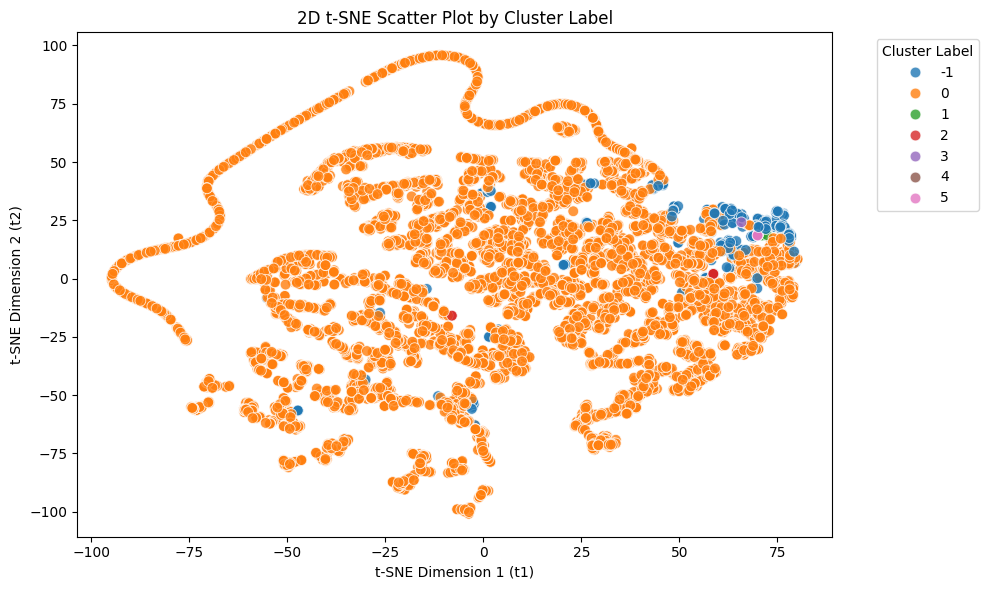
\includegraphics{빅데이터_과제_files/figure-pdf/cell-25-output-1.png}

\section{Question 3}\label{question-3}

\begin{center}
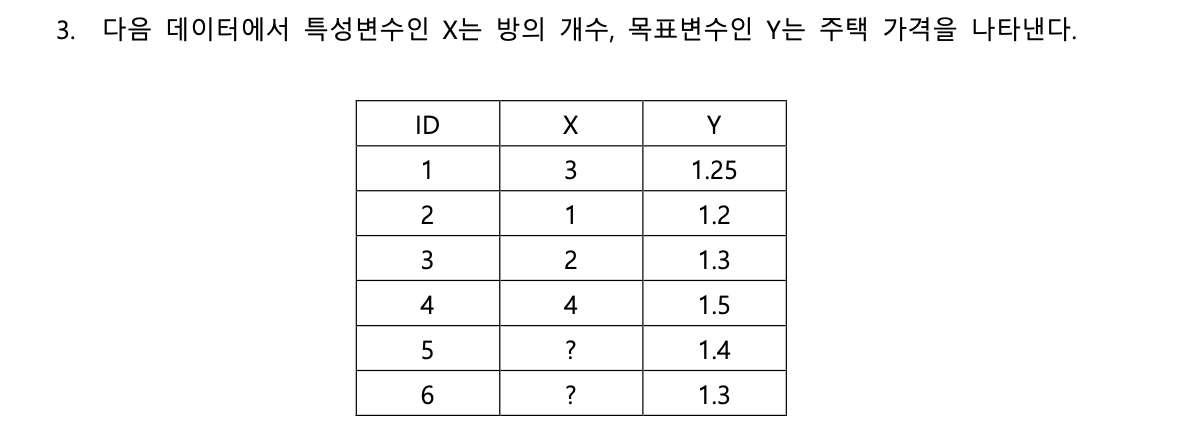
\includegraphics[width=0.7\textwidth,height=\textheight]{image/bigdata3.png}
\end{center}

\subsection{(1)}\label{section-8}

XGBoost 알고리즘을 적용하여 트리를 생성한다고 할 때, 첫번째 트리의 첫
마디에서 최적의 분리기준이 무엇인지를 구하여라. 단, 결측이 아닌 4개의
관찰치(ID 1\textasciitilde ID 4)만 이용할 것. 제곱오차 손실함수를
적용하며, 모델 초기값 𝑓0는 0.5로 두고, 규제 하이퍼 파라미터 𝜆는 0으로
설정할 것. 또한 계산 과정을 상세하게 서술할 것.

\textbf{1. Gradient 및 Hessian 계산}

\begin{itemize}
\tightlist
\item
  손실함수: \((y_i - \hat{y}_i)^2\)
\item
  예측값: \(\hat{y}_i = 0.5\)
\item
  Gradient: \(g_i = \hat{y}_i - y_i = 0.5 - y_i\)
\item
  Hessian: \(h_i = 1\) (제곱오차 손실함수는 상수)
\end{itemize}

\begin{longtable}[]{@{}llll@{}}
\toprule\noalign{}
ID & \(y_i\) & \(g_i\) & \(h_i\) \\
\midrule\noalign{}
\endhead
\bottomrule\noalign{}
\endlastfoot
1 & 1.25 & -0.75 & 1 \\
2 & 1.20 & -0.70 & 1 \\
3 & 1.30 & -0.80 & 1 \\
4 & 1.50 & -1.00 & 1 \\
\end{longtable}

\begin{center}\rule{0.5\linewidth}{0.5pt}\end{center}

\textbf{2. Split 후보 및 Gain 계산}

Gain 공식 (\(\lambda = 0\)):

\[
\text{Gain} = \frac{1}{2} \left[ \frac{G_L^2}{H_L} + \frac{G_R^2}{H_R} - \frac{(G_L + G_R)^2}{H_L + H_R} \right]
\]

\begin{center}\rule{0.5\linewidth}{0.5pt}\end{center}

Split 1: \(X \leq 1.5\)

\begin{itemize}
\tightlist
\item
  Left: ID 2 → \(G_L = -0.70\), \(H_L = 1\)\\
\item
  Right: ID 1, 3, 4 → \(G_R = -2.55\), \(H_R = 3\)
\end{itemize}

\[
\text{Gain}_1 = \frac{1}{2} \left( 0.49 + 2.1675 - 2.640625 \right) = 0.0084
\]

\begin{center}\rule{0.5\linewidth}{0.5pt}\end{center}

Split 2: \(X \leq 2.5\)

\begin{itemize}
\tightlist
\item
  Left: ID 2, 3 → \(G_L = -1.50\), \(H_L = 2\)\\
\item
  Right: ID 1, 4 → \(G_R = -1.75\), \(H_R = 2\)
\end{itemize}

\[
\text{Gain}_2 = \frac{1}{2} \left( 1.125 + 1.53125 - 2.640625 \right) = 0.0078
\]

\begin{center}\rule{0.5\linewidth}{0.5pt}\end{center}

Split 3: \(X \leq 3.5\)

\begin{itemize}
\tightlist
\item
  Left: ID 1, 2, 3 → \(G_L = -2.25\), \(H_L = 3\)\\
\item
  Right: ID 4 → \(G_R = -1.00\), \(H_R = 1\)
\end{itemize}

\[
\text{Gain}_3 = \frac{1}{2} \left( 1.6875 + 1 - 2.640625 \right) = 0.0234
\]

\begin{center}\rule{0.5\linewidth}{0.5pt}\end{center}

\textbf{결론}

\begin{longtable}[]{@{}ll@{}}
\toprule\noalign{}
Split 조건 & Gain \\
\midrule\noalign{}
\endhead
\bottomrule\noalign{}
\endlastfoot
\(X \leq 1.5\) & 0.0084 \\
\(X \leq 2.5\) & 0.0078 \\
\(X \leq 3.5\) & \textbf{0.0234} \\
\end{longtable}

\textbf{최적 분리 기준}: \(X \leq 3.5\)

\subsection{(2)}\label{section-9}

XGBoost 알고리즘을 적용하여 트리를 생성한다고 할 때, 첫번째 트리의 첫
마디에서 X의 값이 결측인 경우는 왼쪽과 오른쪽 자식마디 중 어느 쪽으로
보내야 할지를 결정하여라.

위의 최적 분할 기준 \(X \leq 3.5\)에 따라, 아래 상황임.

\begin{itemize}
\tightlist
\item
  Left: ID 1, 2, 3 → \(G_L = -2.25\), \(H_L = 3\)\\
\item
  Right: ID 4 → \(G_R = -1.00\), \(H_R = 1\)
\end{itemize}

\begin{center}\rule{0.5\linewidth}{0.5pt}\end{center}

\textbf{1. 결측이 ID 5인 경우 (\(Y = 1.4\))}

\begin{itemize}
\tightlist
\item
  \(g_5 = 0.5 - 1.4 = -0.9\), \(h_5 = 1\)
\end{itemize}

\emph{Case A: 왼쪽으로 보낼 경우}

\begin{itemize}
\tightlist
\item
  \(G_L = -3.15\), \(H_L = 4\)
\item
  \(G_R = -1.00\), \(H_R = 1\)
\end{itemize}

\[
\text{Gain}_{5,\text{left}} = \frac{1}{2} \left( \frac{(-3.15)^2}{4} + \frac{(-1)^2}{1} - \frac{(-4.15)^2}{5} \right) = 0.0181
\]

\emph{Case B: 오른쪽으로 보낼 경우}

\begin{itemize}
\tightlist
\item
  \(G_L = -2.25\), \(H_L = 3\)
\item
  \(G_R = -1.9\), \(H_R = 2\)
\end{itemize}

\[
\text{Gain}_{5,\text{right}} = \frac{1}{2} \left( \frac{(-2.25)^2}{3} + \frac{(-1.9)^2}{2} - \frac{(-4.15)^2}{5} \right) = 0.0240
\]

\textbf{결론: 결측값이 ID 5인 경우, 오른쪽이 더 유리함}

\begin{center}\rule{0.5\linewidth}{0.5pt}\end{center}

\textbf{2. 결측이 ID 6인 경우 (\(Y = 1.3\))}

\begin{itemize}
\tightlist
\item
  \(g_6 = 0.5 - 1.3 = -0.8\), \(h_6 = 1\)
\end{itemize}

\emph{Case A: 왼쪽으로 보낼 경우}

\begin{itemize}
\tightlist
\item
  \(G_L = -3.05\), \(H_L = 4\)
\item
  \(G_R = -1.00\), \(H_R = 1\)
\end{itemize}

\[
\text{Gain}_{6,\text{left}} = \frac{1}{2} \left( \frac{(-3.05)^2}{4} + \frac{(-1)^2}{1} - \frac{(-4.05)^2}{5} \right) = 0.0229
\]

\emph{Case B: 오른쪽으로 보낼 경우}

\begin{itemize}
\tightlist
\item
  \(G_L = -2.25\), \(H_L = 3\)
\item
  \(G_R = -1.8\), \(H_R = 2\)
\end{itemize}

\[
\text{Gain}_{6,\text{right}} = \frac{1}{2} \left( \frac{(-2.25)^2}{3} + \frac{(-1.8)^2}{2} - \frac{(-4.05)^2}{5} \right) = 0.0135
\]

\textbf{결론: ID 6은 왼쪽이 더 유리함}

\begin{center}\rule{0.5\linewidth}{0.5pt}\end{center}

\textbf{\emph{요약}}

\begin{longtable}[]{@{}lllll@{}}
\toprule\noalign{}
결측 ID & \(Y\) 값 & 왼쪽 Gain & 오른쪽 Gain & 더 나은 방향 \\
\midrule\noalign{}
\endhead
\bottomrule\noalign{}
\endlastfoot
ID 5 & 1.4 & 0.0181 & 0.0240 & 오른쪽 \\
ID 6 & 1.3 & 0.0229 & 0.0135 & 왼쪽 \\
\end{longtable}

\chapter*{빅데이터와 금융자료분석 프로젝트 (Team
4)}\label{uxbe45uxb370uxc774uxd130uxc640-uxae08uxc735uxc790uxb8ccuxbd84uxc11d-uxd504uxb85cuxc81duxd2b8-team-4}
\addcontentsline{toc}{chapter}{빅데이터와 금융자료분석 프로젝트 (Team
4)}

\markboth{빅데이터와 금융자료분석 프로젝트 (Team 4)}{빅데이터와
금융자료분석 프로젝트 (Team 4)}

\textbf{XGboost 알고리즘을 활용한 은행 대출의 부도 여부 예측 모델 구축}

강상묵(20259013) 김형환(20249132) 유석호(20249264) 이현준(20249349)
최영서(20249430) 최재필(20249433)

\section*{1. 프로젝트 개요}\label{uxd504uxb85cuxc81duxd2b8-uxac1cuxc694}
\addcontentsline{toc}{section}{1. 프로젝트 개요}

\markright{1. 프로젝트 개요}

본 프로젝트는 \textbf{여러 데이터 전처리 기법(결측치, 이상치, 특성공학
등)과 머신러닝 알고리즘(이상치 분류, 차원축소, XGBoost 등)을 실제
금융데이터에 적용}해보고 시사점을 도출하기 위해 작성되었습니다.

이를 위해 미국 Lending Club의 P2P 대출 데이터를 사용하였으며, 전반적인
워크플로우는 아래와 같습니다.

\begin{enumerate}
\def\labelenumi{\arabic{enumi}.}
\tightlist
\item
  데이터의 구조, 특성 파악 (EDA)
\item
  데이터의 전처리 (특성에 따른 칼럼 가공, 문자형 변수 처리, 결측치 및
  이상치 처리, 변수 선택)
\item
  XGBoost 알고리즘을 이용한 대출 연체여부 예측 모델 구축 및 평가

  \begin{itemize}
  \tightlist
  \item
    샘플링, 모델 튜닝, 성과 평가, 변수 중요도 분석(SHAP), Cat/LightGBM
    등 다른 모델과 비교
  \end{itemize}
\end{enumerate}

\section*{2. 데이터의 구조, 특성
(EDA)}\label{uxb370uxc774uxd130uxc758-uxad6cuxc870-uxd2b9uxc131-eda}
\addcontentsline{toc}{section}{2. 데이터의 구조, 특성 (EDA)}

\markright{2. 데이터의 구조, 특성 (EDA)}

\subsection*{데이터의 수집,
기본구조}\label{uxb370uxc774uxd130uxc758-uxc218uxc9d1-uxae30uxbcf8uxad6cuxc870}
\addcontentsline{toc}{subsection}{데이터의 수집, 기본구조}

미국 소재의 P2P 대출 전문은행인 Lending Club의 '07\textasciitilde'20년
대출 데이터를 사용하였습니다. (출처 : Kaggle)

약 40만개의 데이터로, 목적변수인 대출상태를 포함해 전체 27개의
칼럼(수치형 12 + 문자형 15)으로 이루어져있으며, 목적변수는 정상(상환,
Fully paid) 및 부도(연체, Charged off)로 이진분류 문제입니다.

\begin{figure}

\begin{minipage}{0.50\linewidth}
\begin{center}
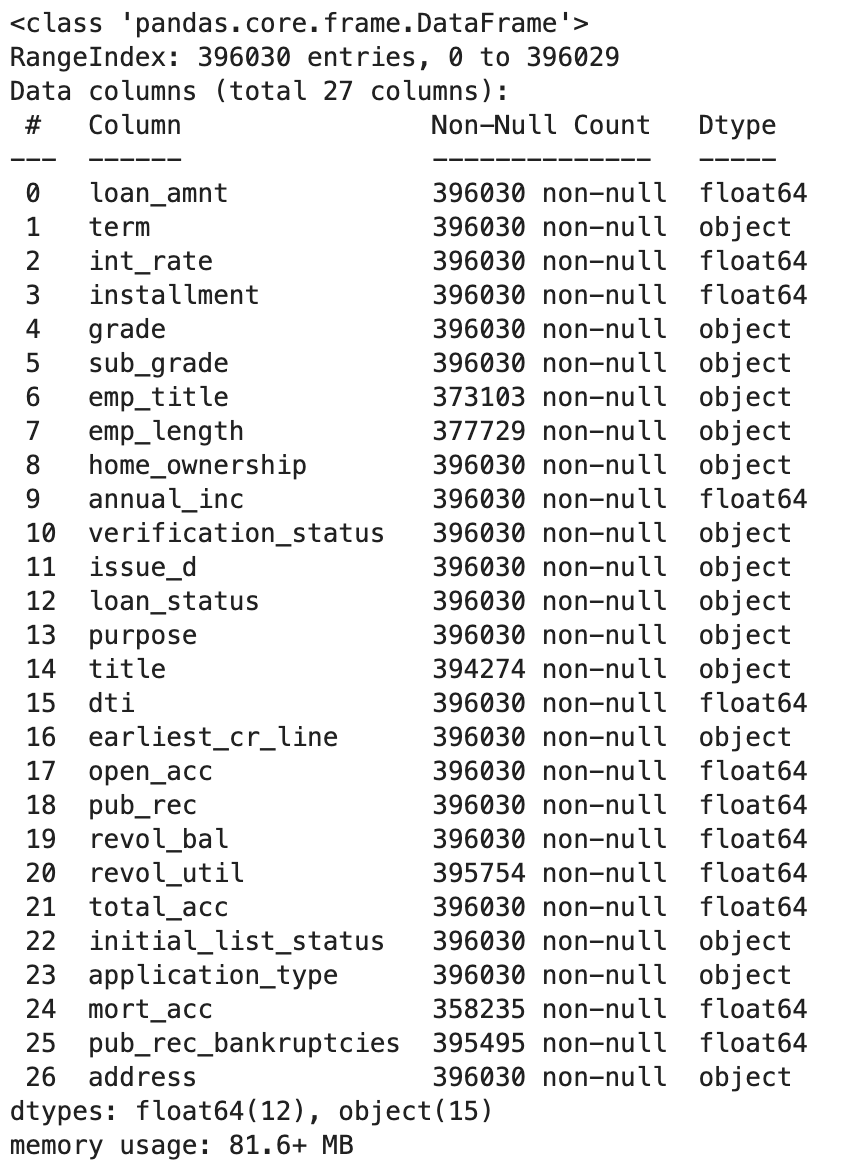
\includegraphics[width=9cm,height=5.5cm]{image/ml1_datainfo.png}
\end{center}
\end{minipage}%
%
\begin{minipage}{0.50\linewidth}
\begin{center}
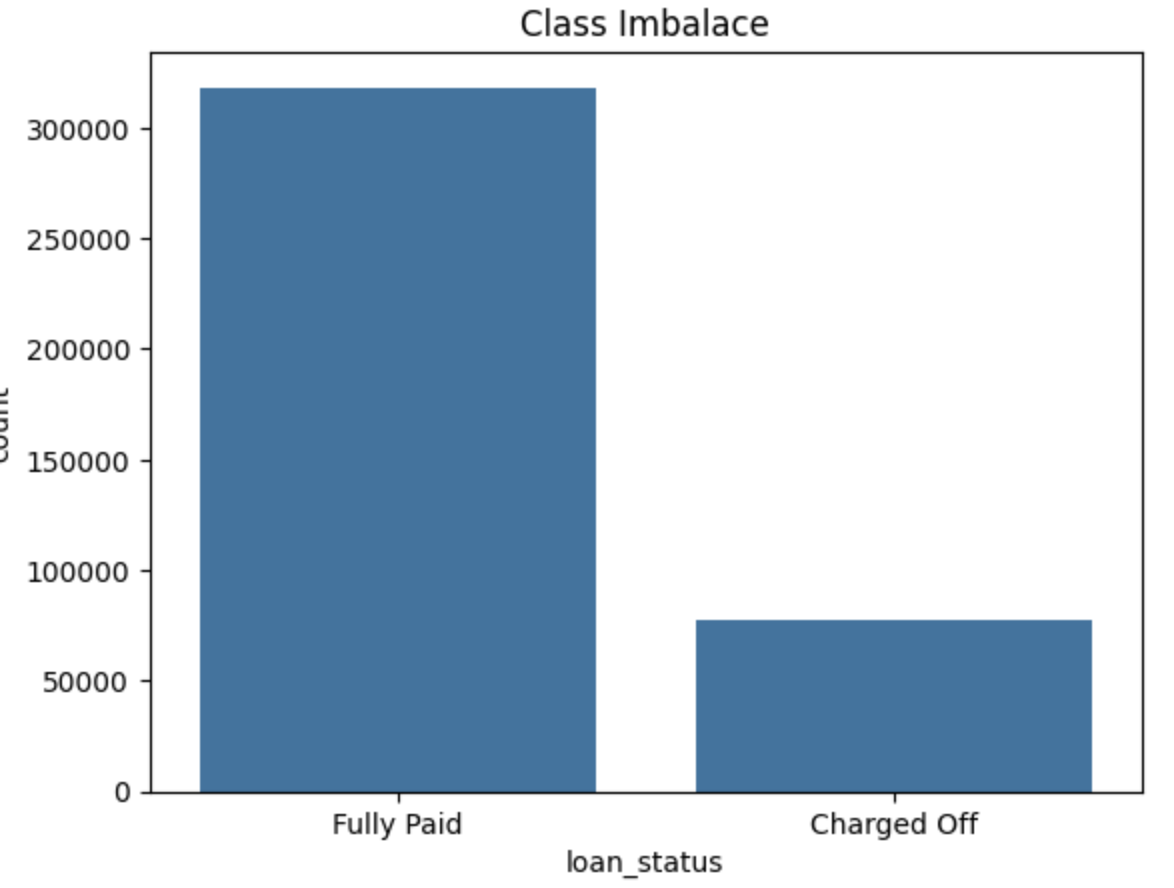
\includegraphics[width=0.8\textwidth,height=\textheight]{image/ml2_classimbal.png}
\end{center}
\end{minipage}%

\end{figure}%

\subsection*{데이터의 특성}\label{uxb370uxc774uxd130uxc758-uxd2b9uxc131}
\addcontentsline{toc}{subsection}{데이터의 특성}

데이터의 각 칼럼별 특징을 알아보고, 적절한 전처리 방법을
탐색해보았습니다.

먼저 \textbf{수치형 변수}입니다. 결측치 및 이상치 처리는 별도 진행
예정으로 따로 다루지 않겠습니다.

\textbf{상관관계 행렬을 Heatmap}으로 살펴보았습니다. 대체적으로 변수들
간 \textbf{상관관계가 미미}하였으며, \textbf{일부 상관계수가 높은
변수}들은 변수선택 과정에서 제외하는 등 \textbf{별도의 전처리 과정을
통해 다중공선성 문제를 해결}할 계획입니다.

\begin{center}
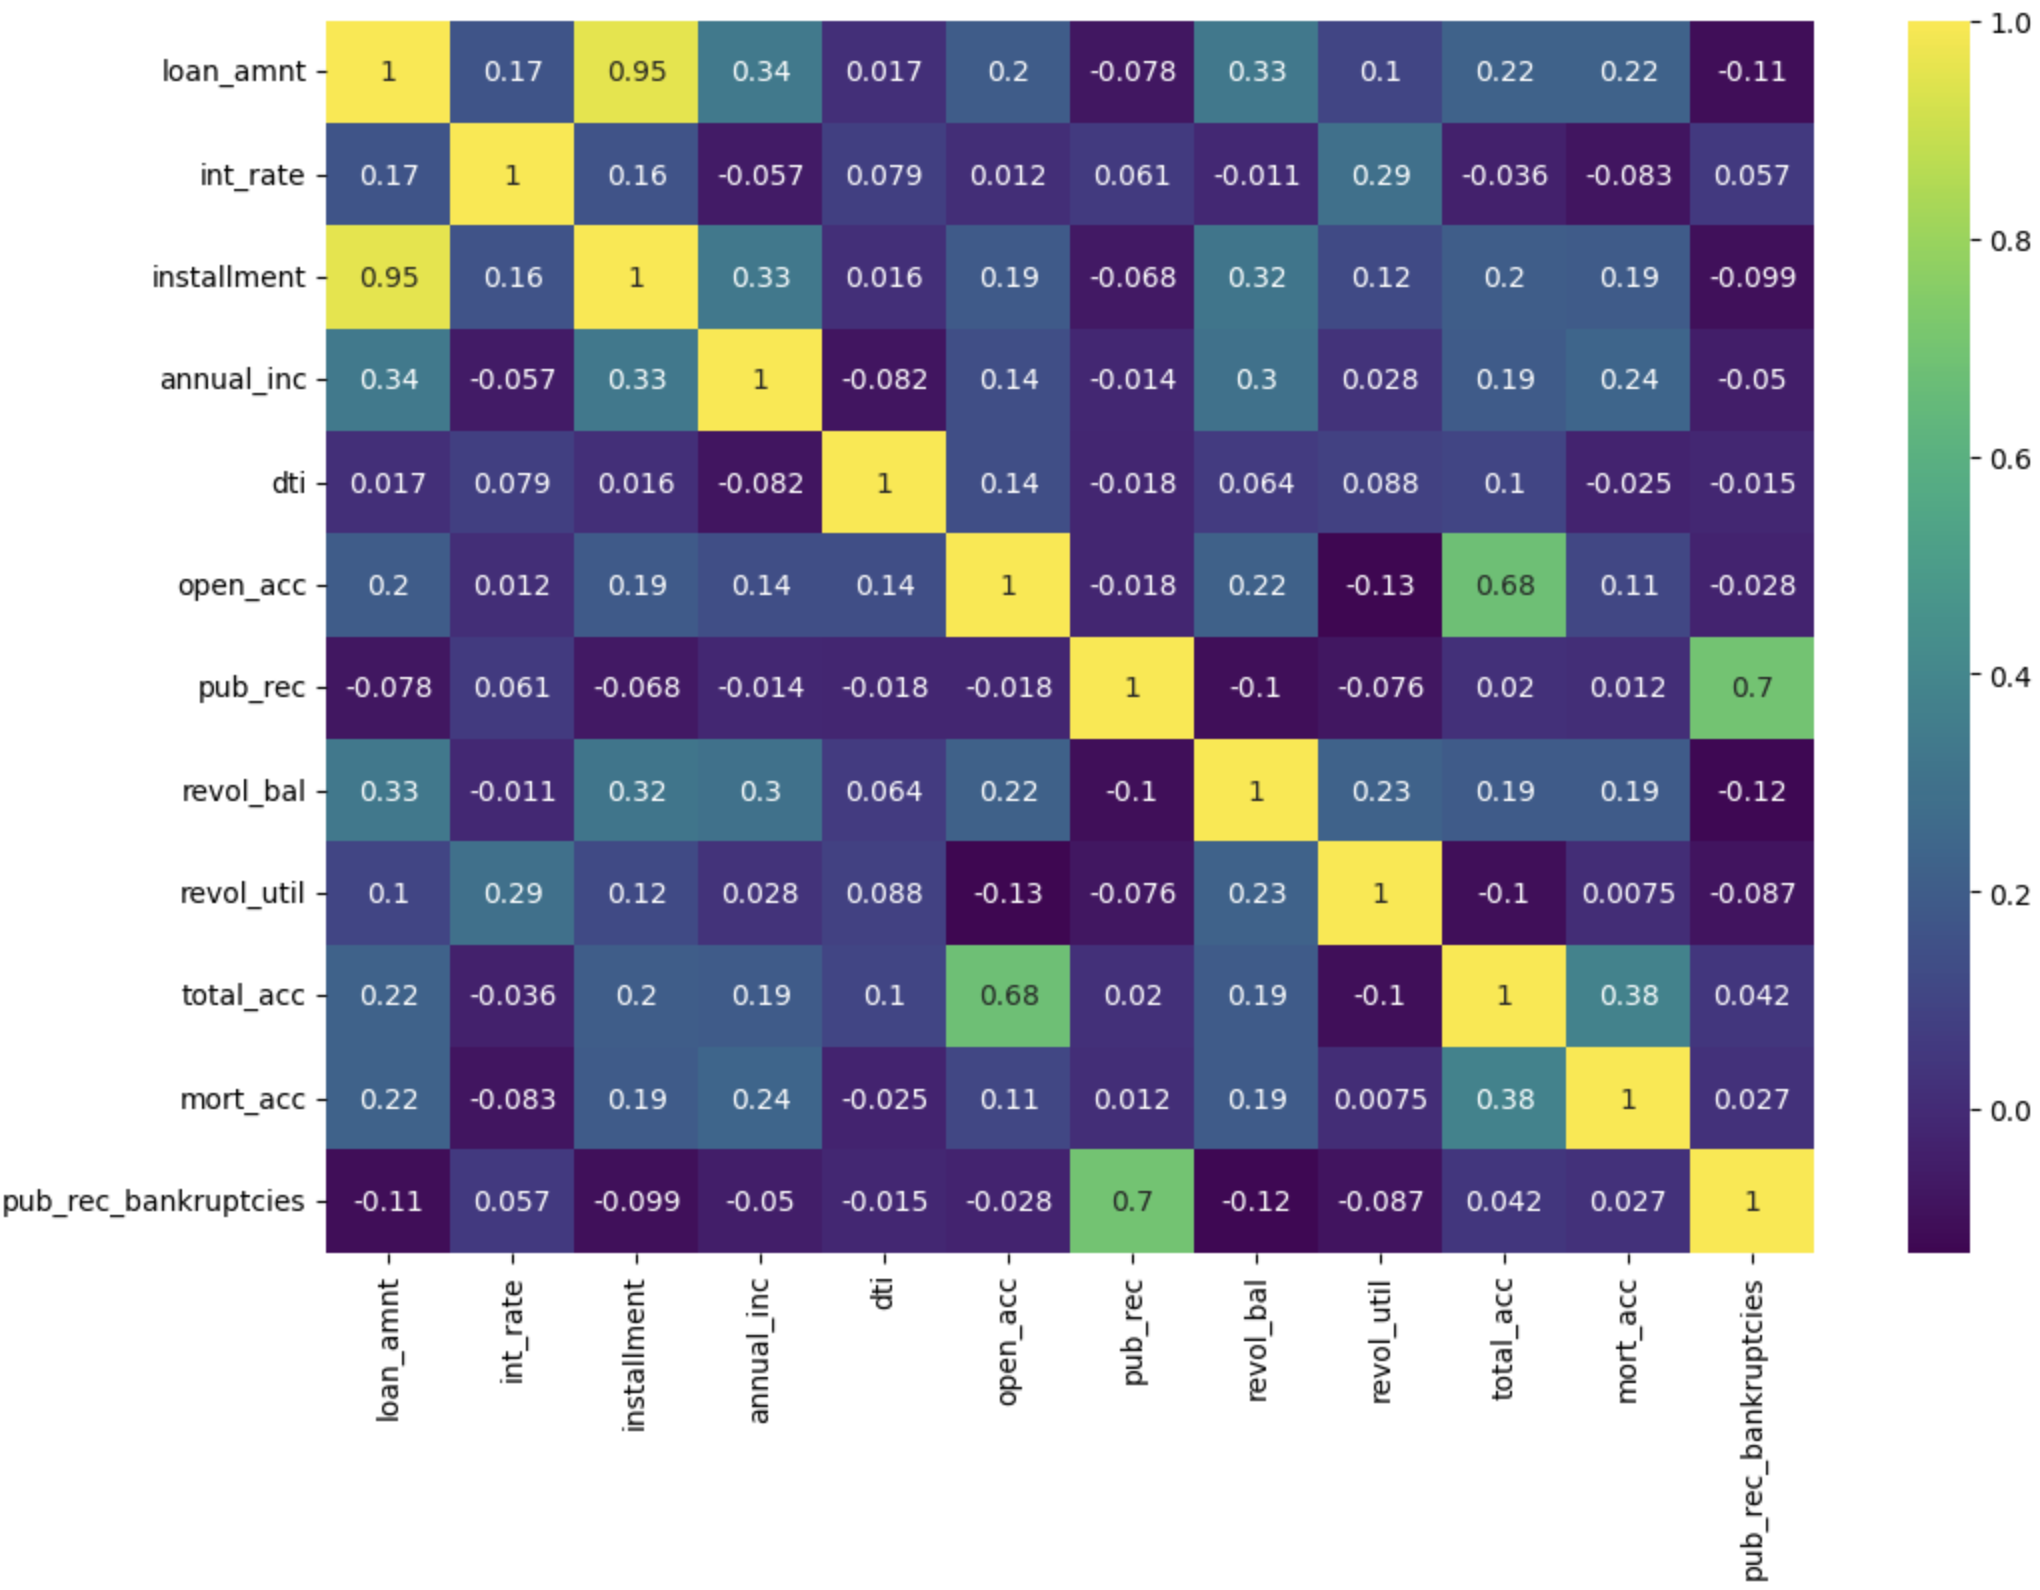
\includegraphics{image/ml3_heatmap.png}
\end{center}

\newpage

다음으로 \textbf{문자형 변수}입니다. 목적변수와 관련이 있는 것으로
보이는 주요 예시만 살펴보겠습니다.

먼저, \textbf{대출기간(term), 집보유형태(home\_ownership),
대출목적(purpose)이 영향}을 미치는 것으로 추정됩니다.

\begin{center}
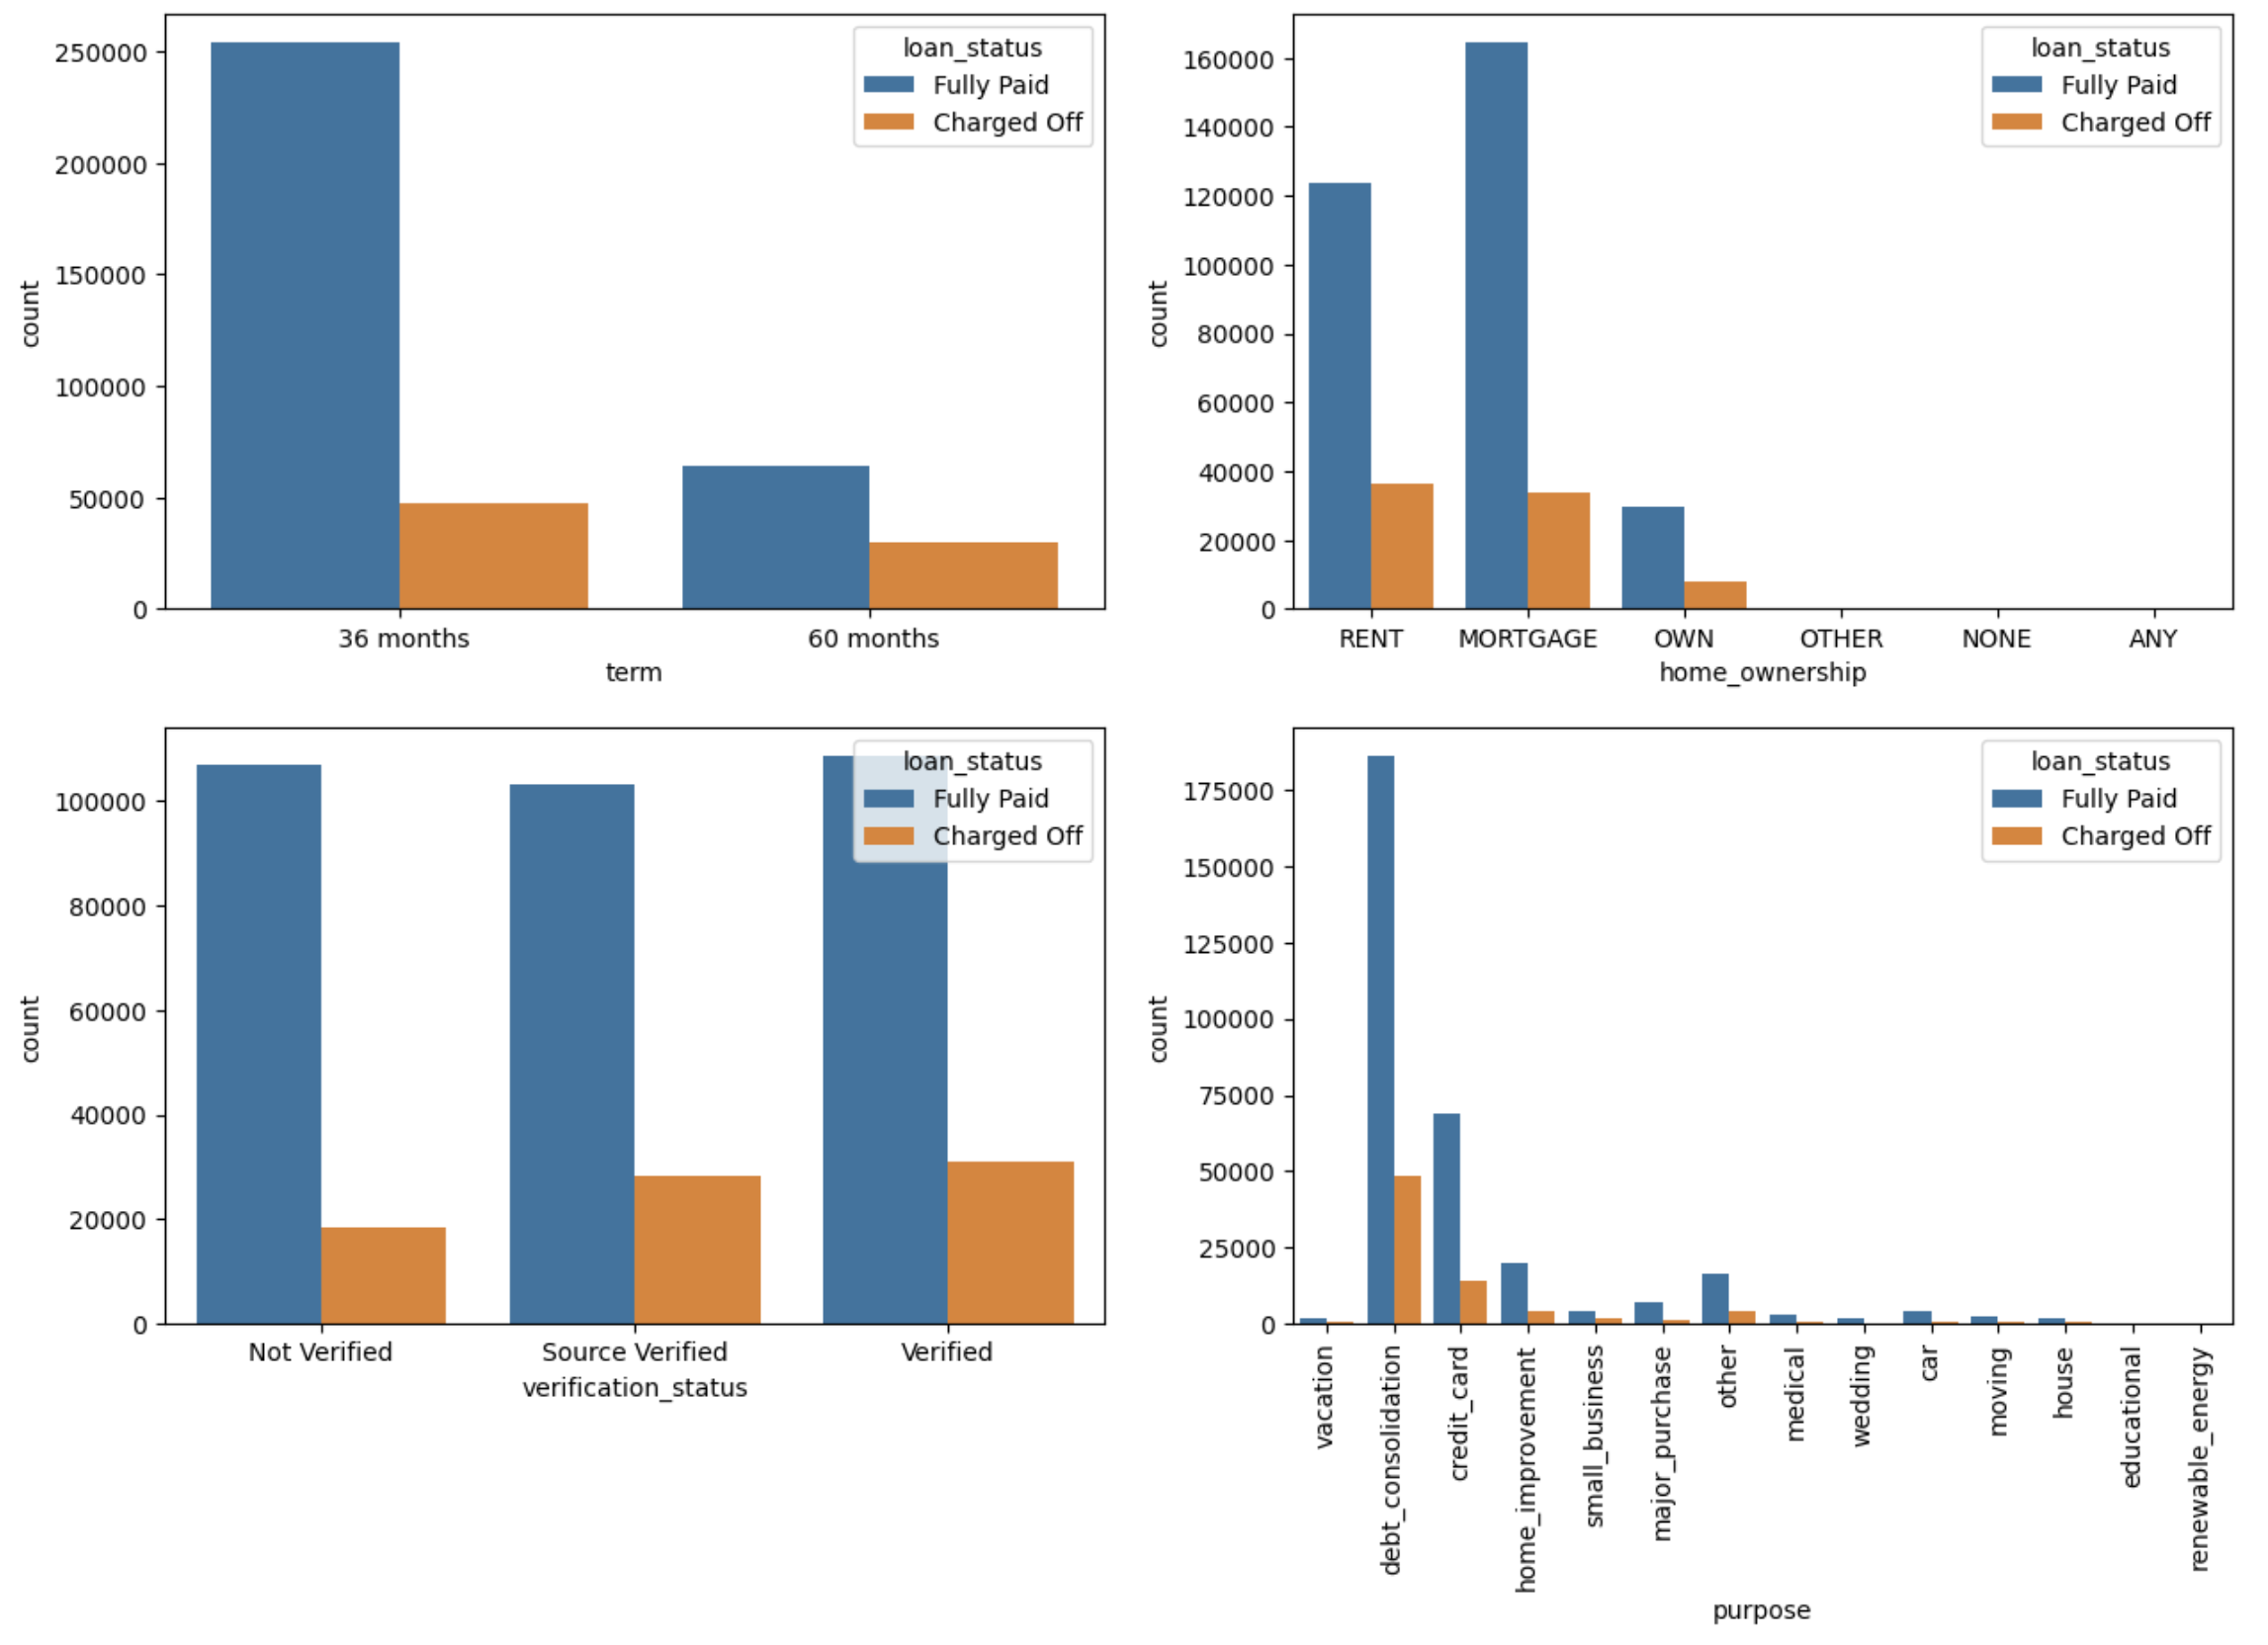
\includegraphics{image/ml5_4plot.png}
\end{center}

다음으로, \textbf{신용등급(A1\textasciitilde G5)에 따라 부도율이
높아지는 추이}를 보였으며, 문자형 변수들 중 \textbf{일부는 고유값이 너무
많아 분석에서 제외}하는 것이 효과적일 것으로 보입니다.

\begin{figure}

\begin{minipage}{0.50\linewidth}
\begin{center}
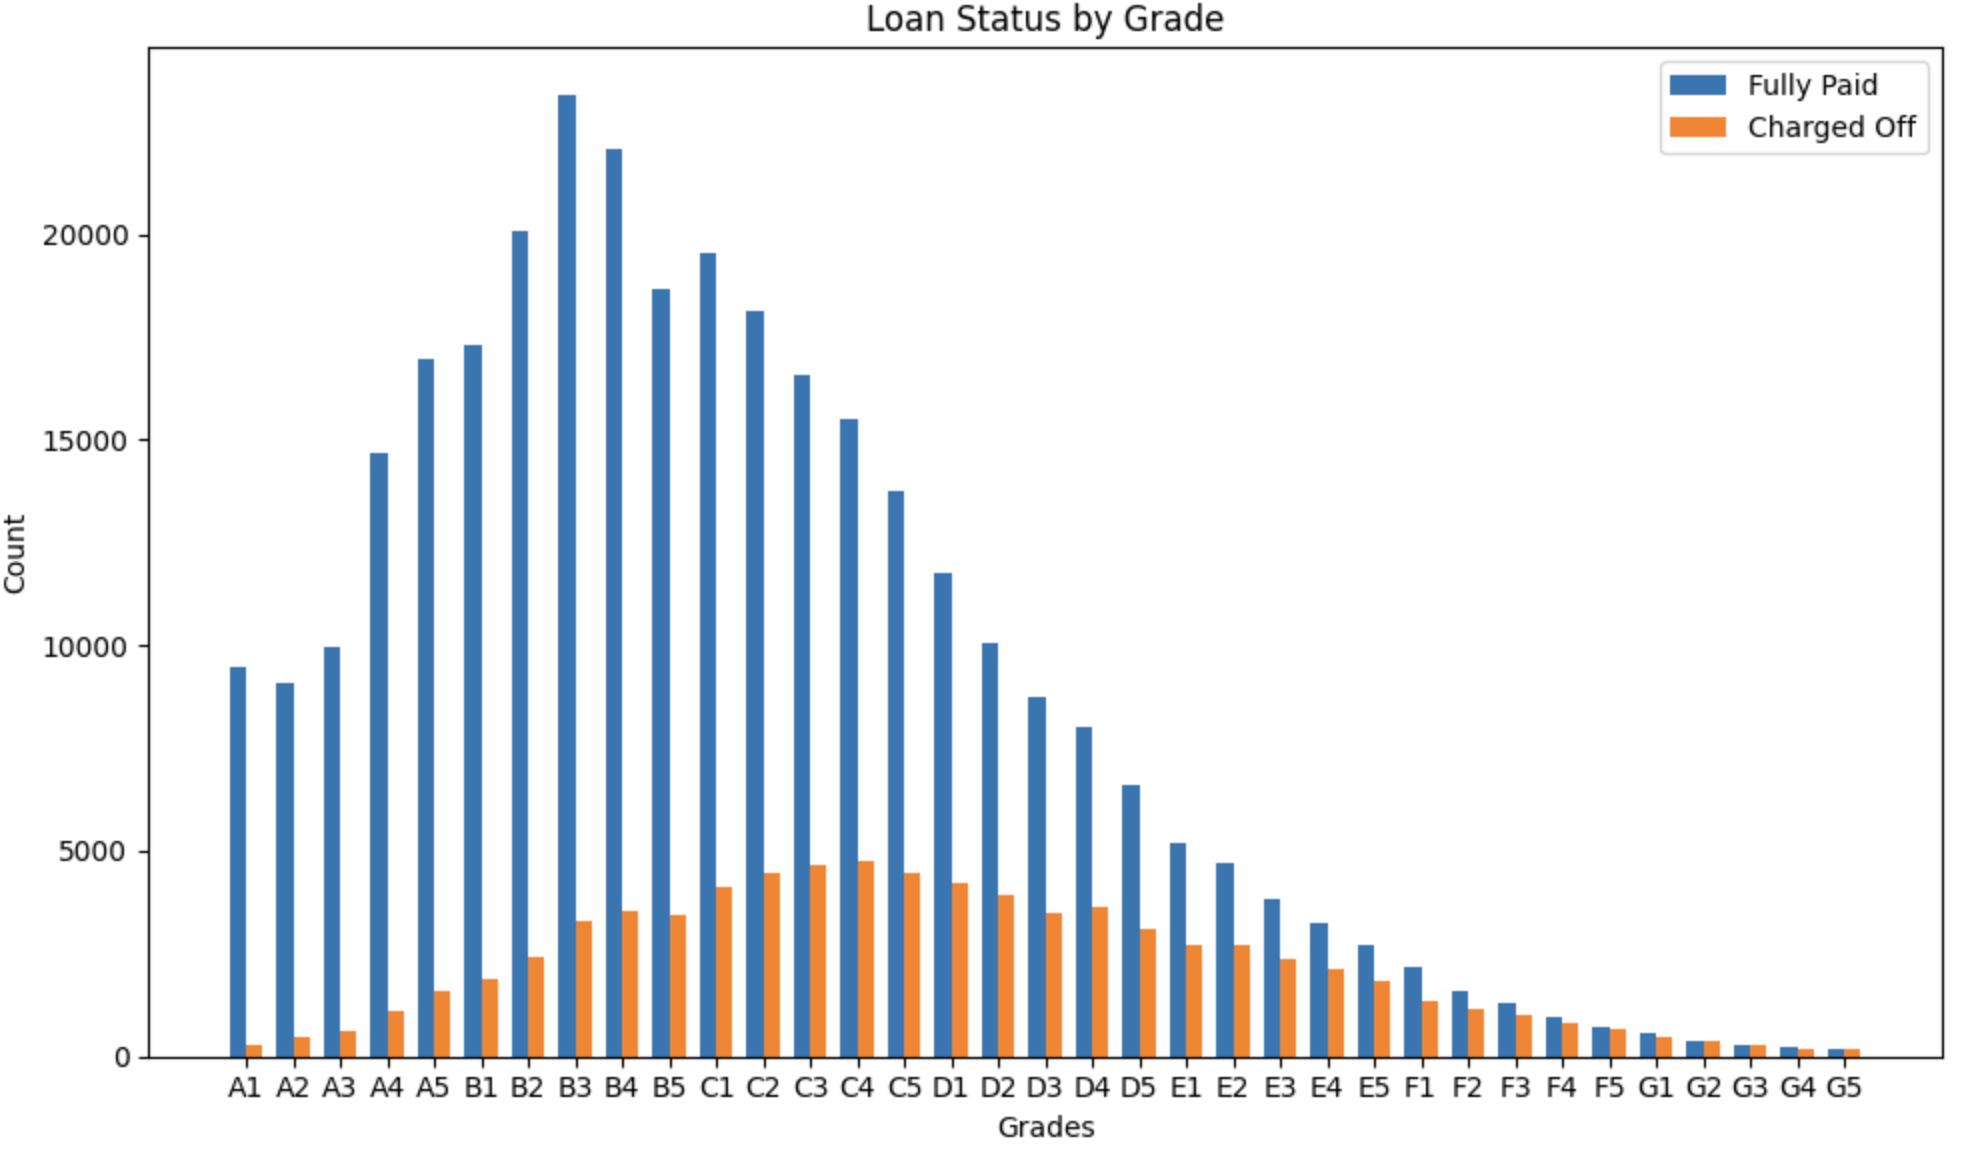
\includegraphics{image/ml4_grade.png}
\end{center}
\end{minipage}%
%
\begin{minipage}{0.50\linewidth}
\begin{center}
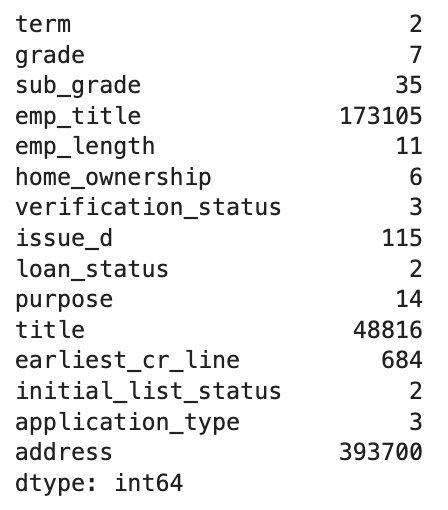
\includegraphics[width=0.5\textwidth,height=\textheight]{image/ml6_category.png}
\end{center}
\end{minipage}%

\end{figure}%

\newpage

\section*{3. 데이터의
전처리}\label{uxb370uxc774uxd130uxc758-uxc804uxcc98uxb9ac}
\addcontentsline{toc}{section}{3. 데이터의 전처리}

\markright{3. 데이터의 전처리}

데이터의 전처리는 아래의 과정으로 실시하였습니다.

\begin{enumerate}
\def\labelenumi{\arabic{enumi}.}
\tightlist
\item
  분석에 적합하도록 칼럼 변환 및 통합, 제거

  \begin{itemize}
  \tightlist
  \item
    변환/통합 : 주소(address)는 우편번호(zip\_code)만 추출하고 제거,
    대출기간(term, 36month 등)은 수치형으로 변환, 집
    소유여부(home\_ownership)의 극소수값들은 Other로 통합
  \item
    불필요한 noise 방지를 위해 100개 이상의 고유값을 가진 칼럼 제거 :
    직업(title), 직업글자수(emp\_title), 발행일(issue\_d),
    최초연도(earliest\_cr\_line)
  \item
    다른 변수와 중복되거나 추론 가능한 칼럼 제거 :
    신용점수-대분류(grade), 근속연수(emp\_length)
  \end{itemize}
\item
  문자형 변수 처리 : 순서가 있거나 이진변수인 경우 라벨인코딩, 단순
  점주인 경우 원핫인코딩 적용

  \begin{itemize}
  \tightlist
  \item
    라벨인코딩 : 목적변수(이진), 신용점수(순서 존재) / 원핫인코딩 :
    이외의 문자형 변수
  \end{itemize}
\item
  수치형 변수의 결측치 및 이상치 처리 : 중간값 처리 및 1\% 이상치 제거

  \begin{itemize}
  \tightlist
  \item
    결측치 : 변수간 상관관계가 미미하고, 이후 Boruta를 적용 예정이므로
    예측형 모델보다는 중간값을 채택
  \item
    이상치 : 고차원, 많은 샘플(약 40만)을 고려, 분포에 대한 가정이
    불필요한 Isolation forest 기법 채택
  \end{itemize}
\item
  변수 선택을 통해 분석에 적합한 최종 데이터 가공 : Boruta 알고리즘 적용

  \begin{itemize}
  \tightlist
  \item
    일부 변수간 상관관계가 존재하는 점을 고려, 최적의 변수 조합을 찾고자
    Boruta 알고리즘 채택
  \item
    원핫인코딩 대상 변수를 제외한 13개(수치형+라벨)에 알고리즘을 적용한
    결과 11개의 변수를 선택하였고, 원핫인코딩 대상 변수와 결합하여 최종
    데이터 구성
  \end{itemize}
\end{enumerate}

\begin{tcolorbox}[enhanced jigsaw, bottomtitle=1mm, breakable, coltitle=black, opacityback=0, titlerule=0mm, left=2mm, colbacktitle=quarto-callout-note-color!10!white, toptitle=1mm, colframe=quarto-callout-note-color-frame, bottomrule=.15mm, opacitybacktitle=0.6, leftrule=.75mm, title=\textcolor{quarto-callout-note-color}{\faInfo}\hspace{0.5em}{Isolation Forest 검증(T-SNE 적용) 및 최종 데이터 구성}, arc=.35mm, toprule=.15mm, rightrule=.15mm, colback=white]

수치형 변수에 \textbf{T-SNE를 적용하여 3차원으로 축소}한 결과,
\textbf{이상치 제거(Isolation Forest)가 적절히 작동}하였으며,
\textbf{Boruta 알고리즘으로 변수 선택}까지 마친 후 \textbf{최종
데이터}는 \textbf{7개의 문자형 변수}(원핫인코딩 6 + 라벨인코딩 1) 및
\textbf{9개의 수치형 변수}, \textbf{1개의 목적변수(이진분류)}로 구성되어
있습니다.

\begin{figure}[H]

\begin{minipage}{0.50\linewidth}
\begin{center}
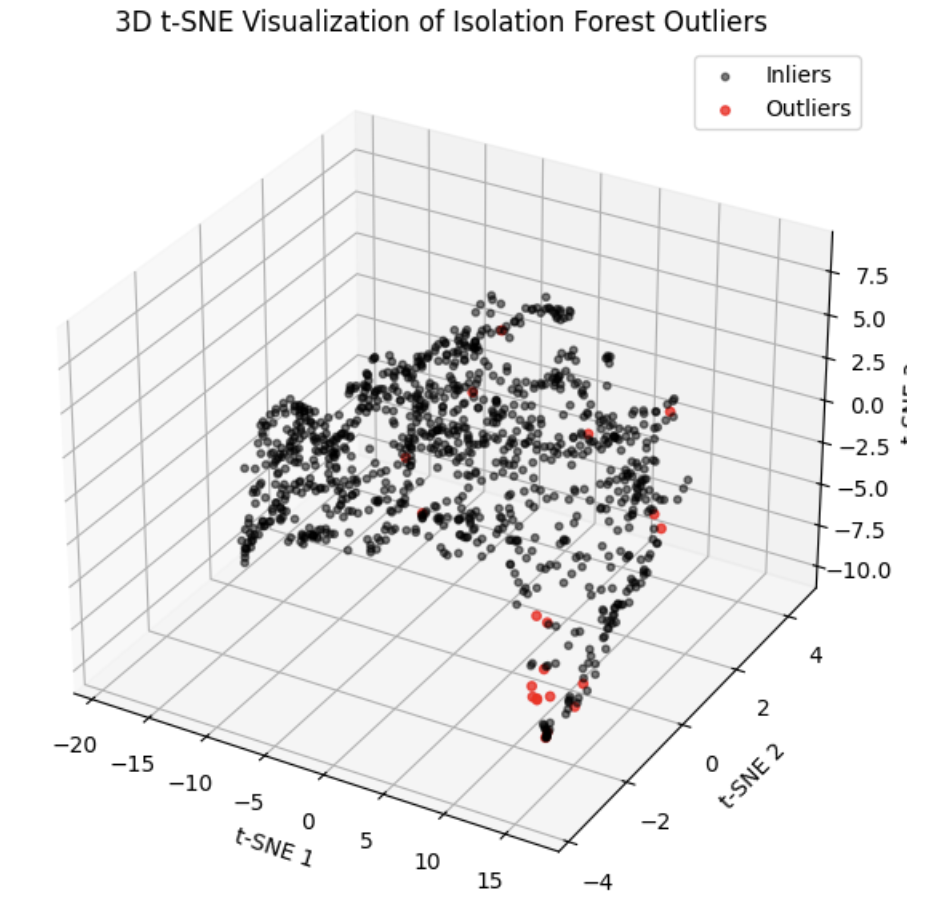
\includegraphics[width=0.8\textwidth,height=\textheight]{image/ml7-1.png}
\end{center}
\end{minipage}%
%
\begin{minipage}{0.50\linewidth}
\begin{center}
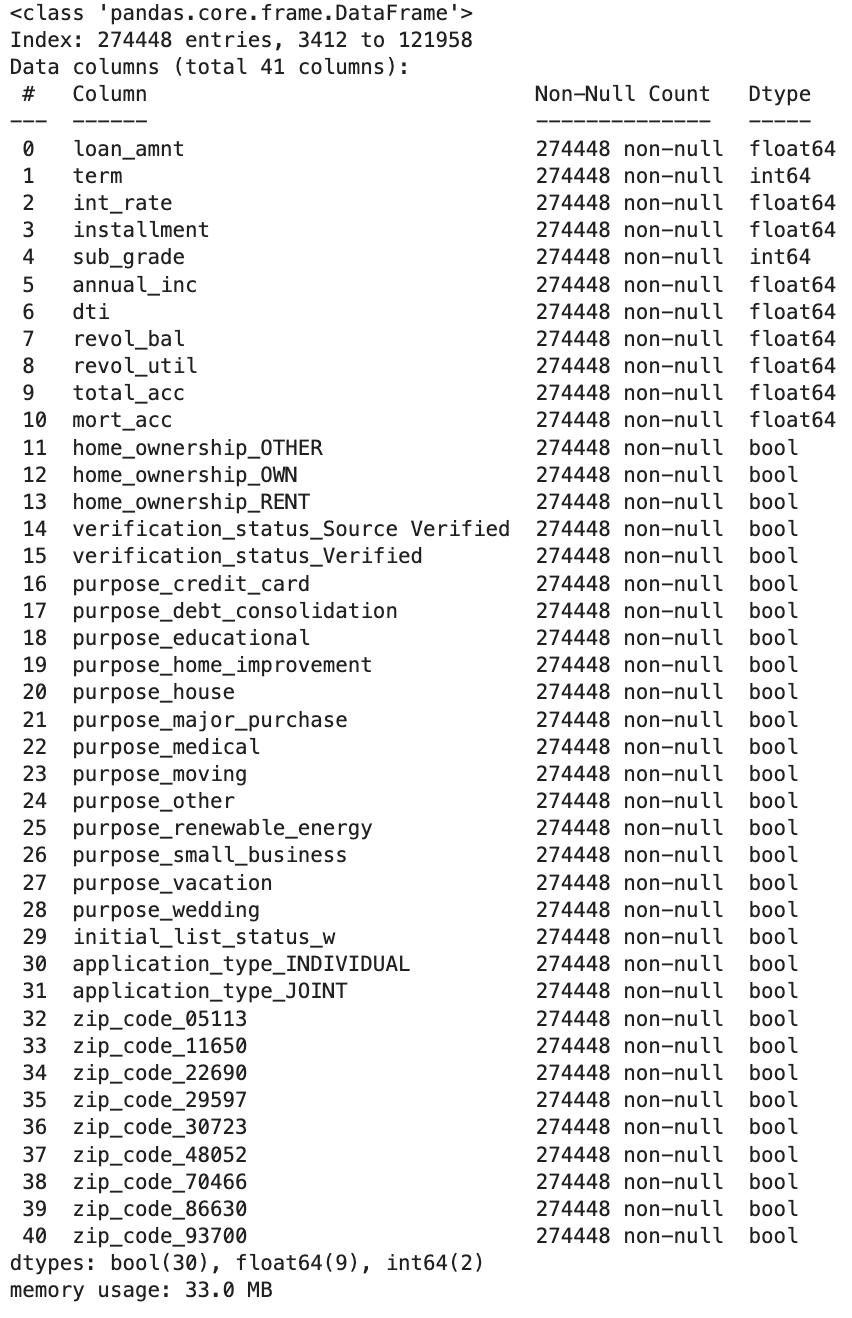
\includegraphics[width=0.55\textwidth,height=\textheight]{image/ml8_finaldata.png}
\end{center}
\end{minipage}%

\end{figure}%

\end{tcolorbox}

\newpage

\section*{4. 대출 연체여부 예측 모델 구축 및
평가}\label{uxb300uxcd9c-uxc5f0uxccb4uxc5ecuxbd80-uxc608uxce21-uxbaa8uxb378-uxad6cuxcd95-uxbc0f-uxd3c9uxac00}
\addcontentsline{toc}{section}{4. 대출 연체여부 예측 모델 구축 및 평가}

\markright{4. 대출 연체여부 예측 모델 구축 및 평가}

\subsection*{ADASYN을 이용한
오버샘플링}\label{adasynuxc744-uxc774uxc6a9uxd55c-uxc624uxbc84uxc0d8uxd50cuxb9c1}
\addcontentsline{toc}{subsection}{ADASYN을 이용한 오버샘플링}

모델링에 앞서, 클래스 불균형 문제는 \textbf{ADASYN을 통한
오버샘플링}으로 해결하였습니다. 과대평가, 과적합을 방지하고 \textbf{검증
무결성을 위해 CV 과정의 훈련 데이터에만 오버샘플링}하였으며,
(\texttt{imblearn.pipeline} 활용) 이를 통해 \textbf{검증은 항상
원본데이터로만 진행}됩니다.

\subsection*{XGBoost 모델 구축}\label{xgboost-uxbaa8uxb378-uxad6cuxcd95}
\addcontentsline{toc}{subsection}{XGBoost 모델 구축}

앞서 구성한 40개 변수로 \textbf{``대출 연체 여부''를 예측하는 모델을
XGBoost 알고리즘}을 통해 구축하였으며, \textbf{모델 튜닝은 2단계 최적화
접근법을 적용}하였습니다. 이러한 방식은 \textbf{과적합을 방지하고 정해진
계산자원 하에서 최대한 공정하게 파라미터를 비교}할 수 있는 장점이
있습니다.

\textbf{1단계: 초기 하이퍼파라미터 탐색} - 상대적으로 높은 학습률(0.1)과
고정된 n\_estimators 값으로 하이퍼파라미터 조합을 탐색 - 각 조합이
동일한 학습 기회(같은 트리 개수)를 갖도록 보장 (CV 내에서 ADASYN
오버샘플링 적용)

\textbf{2단계: 최적 모델 미세 조정} - 1단계에서 찾은 최적
하이퍼파라미터에 낮은 학습률(0.01)과 높은 n\_estimators(10000) 적용 -
조기종료를 적용(50)하여 최적의 트리 개수 결정하고, 전체 훈련/검증
데이터를 사용하여 모델 학습

\begin{figure}[H]

{\centering 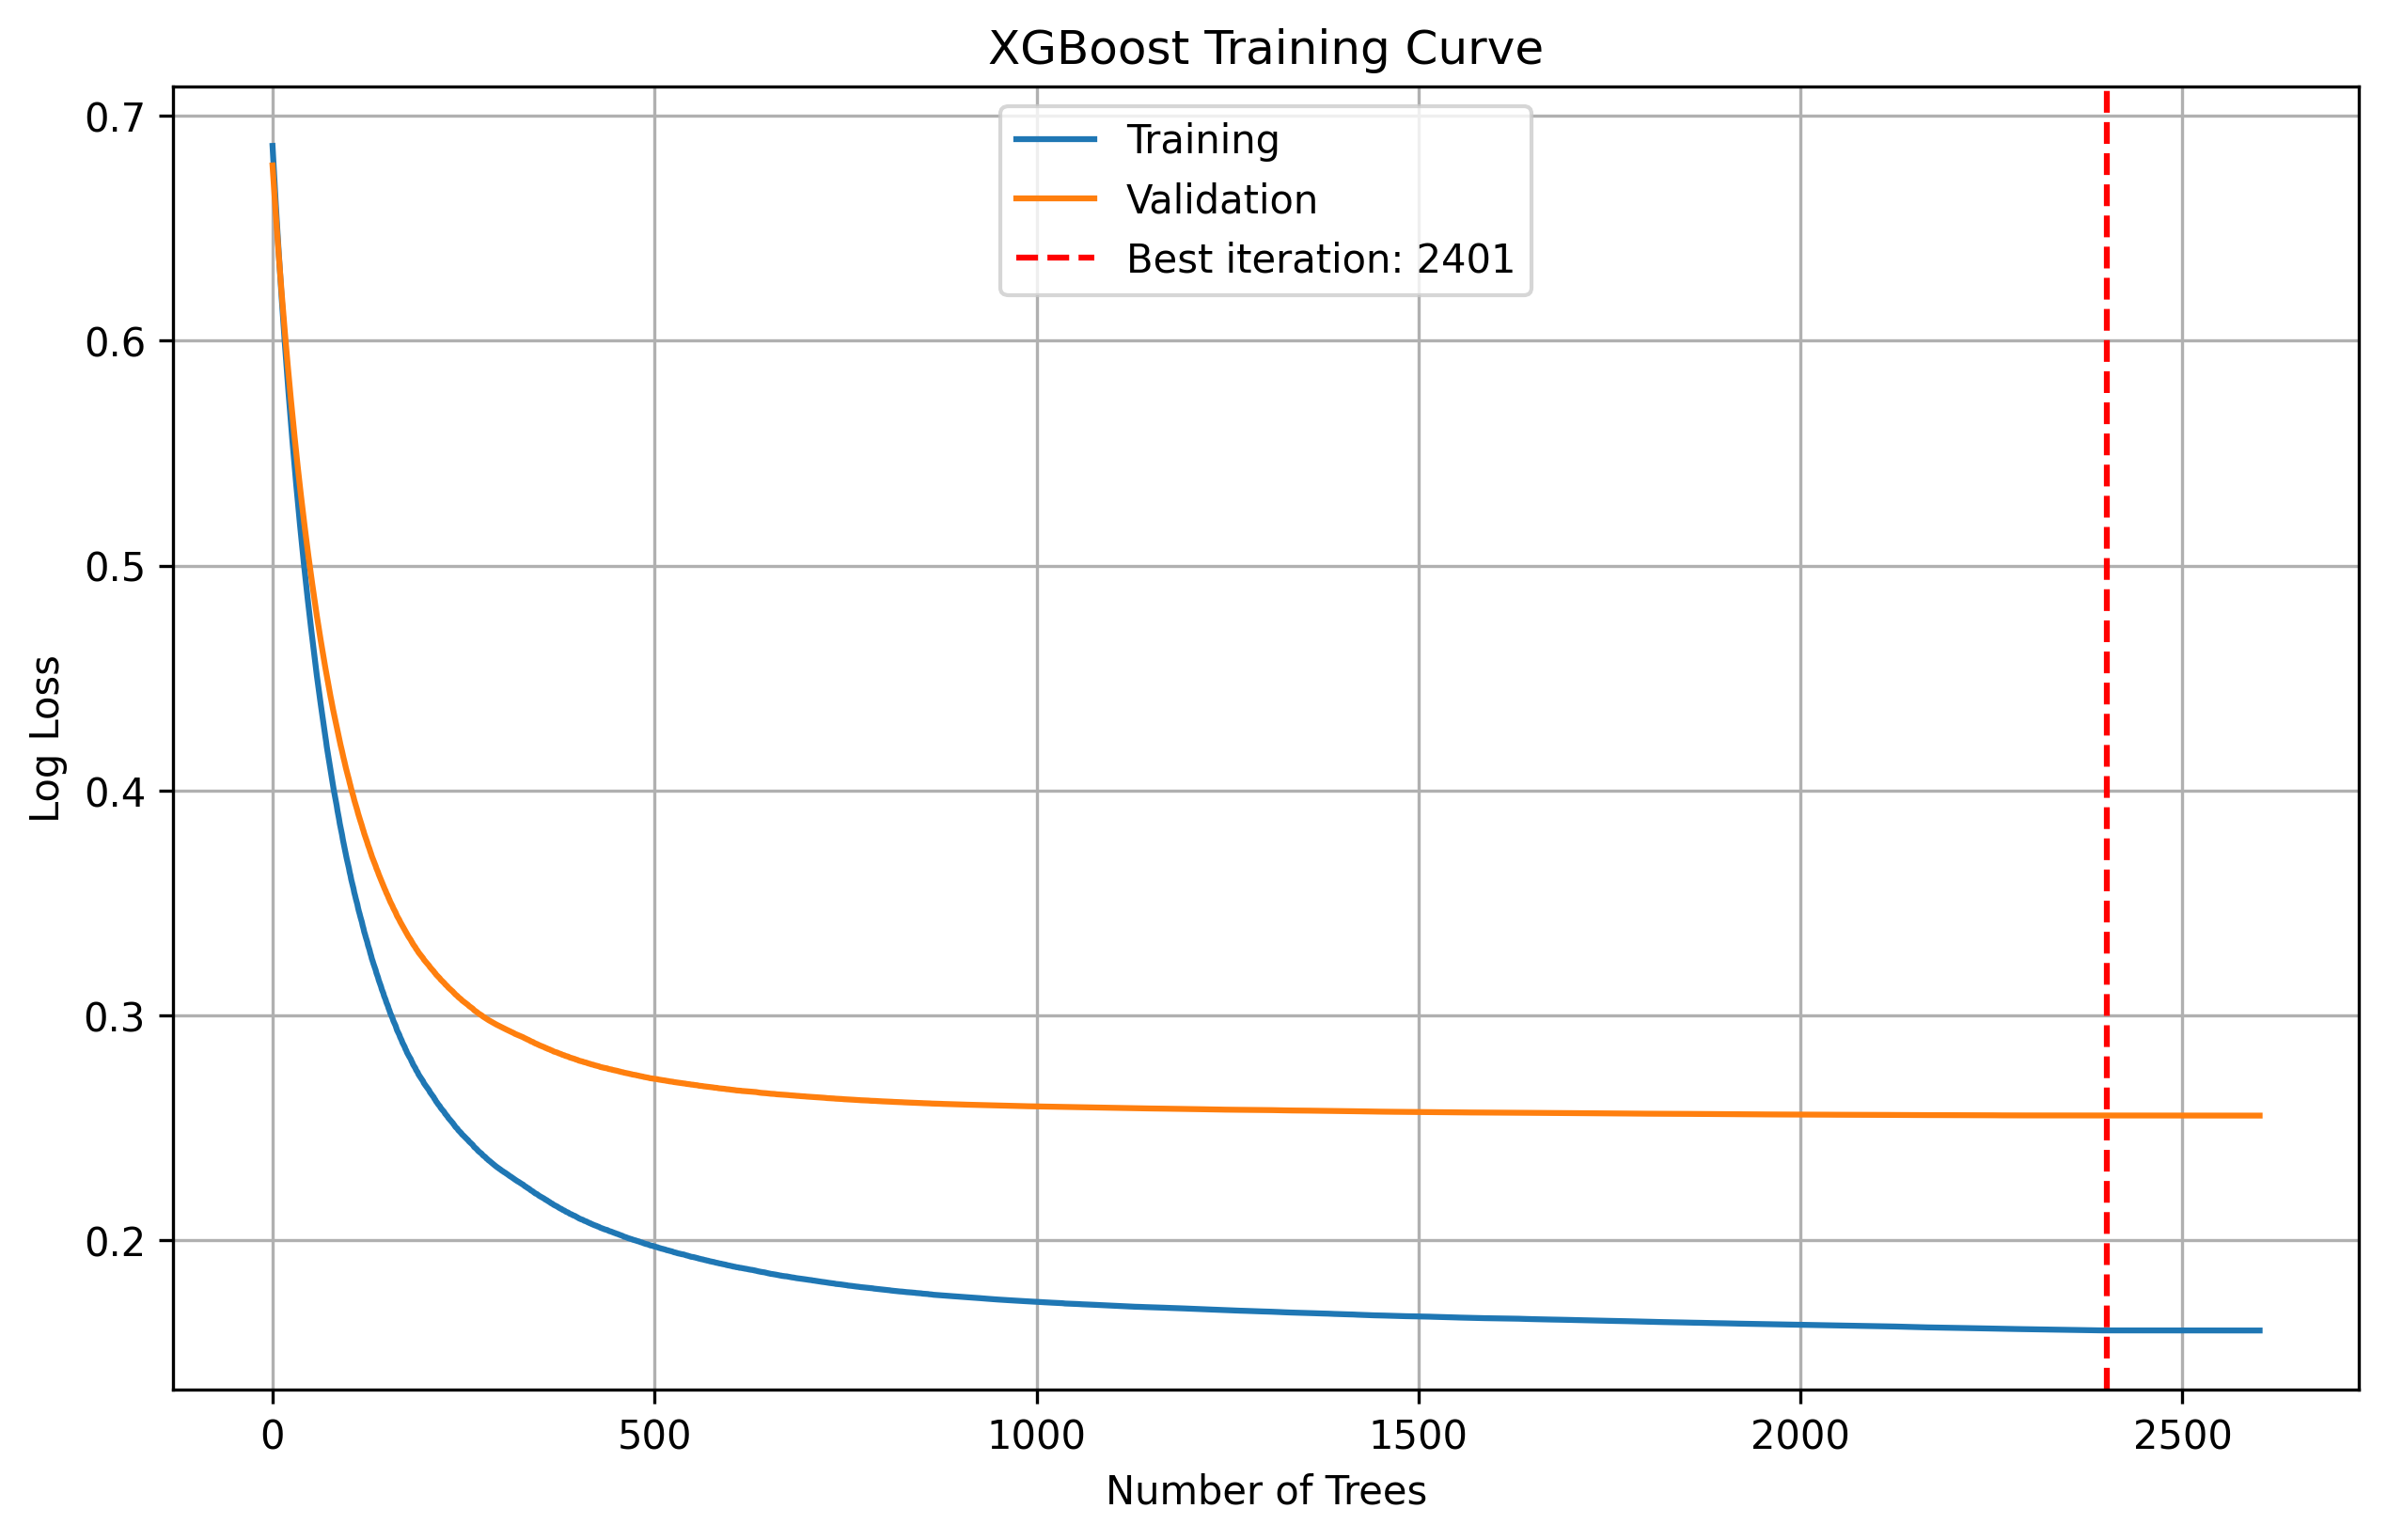
\includegraphics[width=0.7\textwidth,height=\textheight]{plots/learning_curve.png}

}

\caption{2단계 접근법의 최종 모델 학습곡선}

\end{figure}%

\subsection*{모델 일반화성능
평가}\label{uxbaa8uxb378-uxc77cuxbc18uxd654uxc131uxb2a5-uxd3c9uxac00}
\addcontentsline{toc}{subsection}{모델 일반화성능 평가}

클래스 불균형 문제를 고려하여 최종 모델의 \textbf{일반화 성능을
F1-Score를 중심}으로 평가하도록 하겠습니다. \textbf{F1-score는 약 0.94,
ROC-AUC는 약 0.91로 실제 연체 여부를 잘 예측}하는 것으로 나타났습니다.

특히, 모델 튜닝 과정에서 1단계 하이퍼파라미터 탐색시 최고 F1-Score가
0.93544였는데, 일반화 성능은 그와 동일한 수준이므로 \textbf{과적합
방지를 위한 2단계 최적화 기법이 효과적}인 것을 알 수 있습니다.

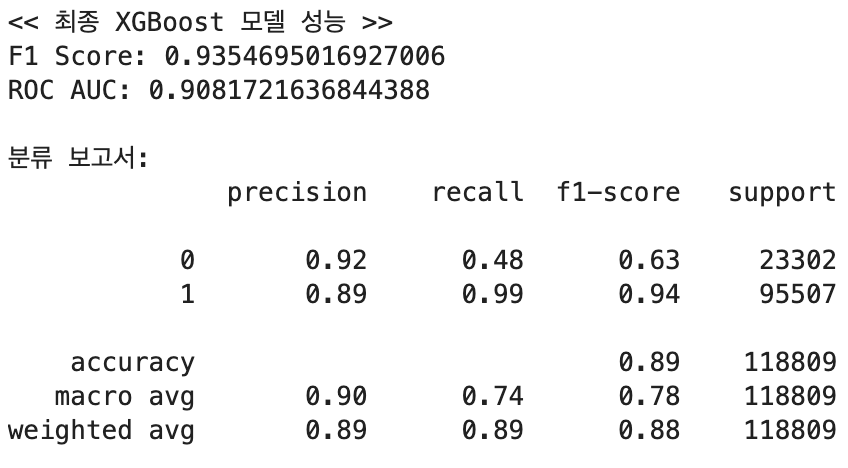
\includegraphics[width=0.6\textwidth,height=\textheight]{image/ml11_best.png}

\begin{tcolorbox}[enhanced jigsaw, bottomtitle=1mm, breakable, coltitle=black, opacityback=0, titlerule=0mm, left=2mm, colbacktitle=quarto-callout-note-color!10!white, toptitle=1mm, colframe=quarto-callout-note-color-frame, bottomrule=.15mm, opacitybacktitle=0.6, leftrule=.75mm, title=\textcolor{quarto-callout-note-color}{\faInfo}\hspace{0.5em}{여러 Gradiant boosting 계열의 알고리즘과 비교}, arc=.35mm, toprule=.15mm, rightrule=.15mm, colback=white]

주로 사용한 XGBoost 이외에도 다양한 Gradiant boosting 계열 및 앙상블
알고리즘이 존재합니다.

\begin{itemize}
\tightlist
\item
  \textbf{XGBoost}: Regularization과 트리 구조 최적화에 강점을 가진
  Gradient Boosting 모델 \textbar{}
\item
  \textbf{CatBoost}: 범주형 변수 자동 인식 기능이 있는 Gradient Boosting
  기반 모델
\item
  \textbf{LightGBM}: 빠른 학습 속도와 낮은 메모리 사용의 Gradient
  Boosting 기반 모델
\item
  \textbf{Soft Voting}: CatBoost, LightGBM의 예측 확률 평균을 통한
  결합(앙상블) 모델
\item
  \textbf{Stacking}: CatBoost, LightGBM의 예측 결과를 Logistic
  Regression에 전달하는 메타 모델 기반 앙상블
\end{itemize}

XGBoost와 유사한 방식으로 각 모델을 튜닝, 훈련하였으며
\textbf{일반화성능은 유사한 수준}이였습니다. F1-Score는 앙상블(Soft
Voting) 모델이, ROC-AUC 점수는 XGBoost가 가장 우수하였습니다.

\begin{longtable}[]{@{}llllll@{}}
\toprule\noalign{}
모델 & F1 Score & ROC AUC & 모델 & F1 Score & ROC AUC \\
\midrule\noalign{}
\endhead
\bottomrule\noalign{}
\endlastfoot
\textbf{CatBoost} & 0.9355 & 0.9073 & \textbf{Soft Voting} & 0.9356 &
0.9072 \\
\textbf{LightGBM} & 0.9353 & 0.9066 & \textbf{Stacking} & 0.9330 &
0.9072 \\
\end{longtable}

\end{tcolorbox}

그러나, \textbf{샘플이 적은 ``부도''인 경우, 예측 성능이 다소 떨어지는
모습}이 관측되었습니다.

\textbf{부도의 절반 이상이 정상으로 분류}되었으며 모든 모델에 동일한
문제가 있는 것으로 볼 때, \textbf{데이터의 한계}인 것으로 보입니다. 또는
\textbf{신경망 계열을 적용해보는 것도 개선방법}이 될 수 있습니다.

\begin{figure}

\begin{minipage}{0.50\linewidth}

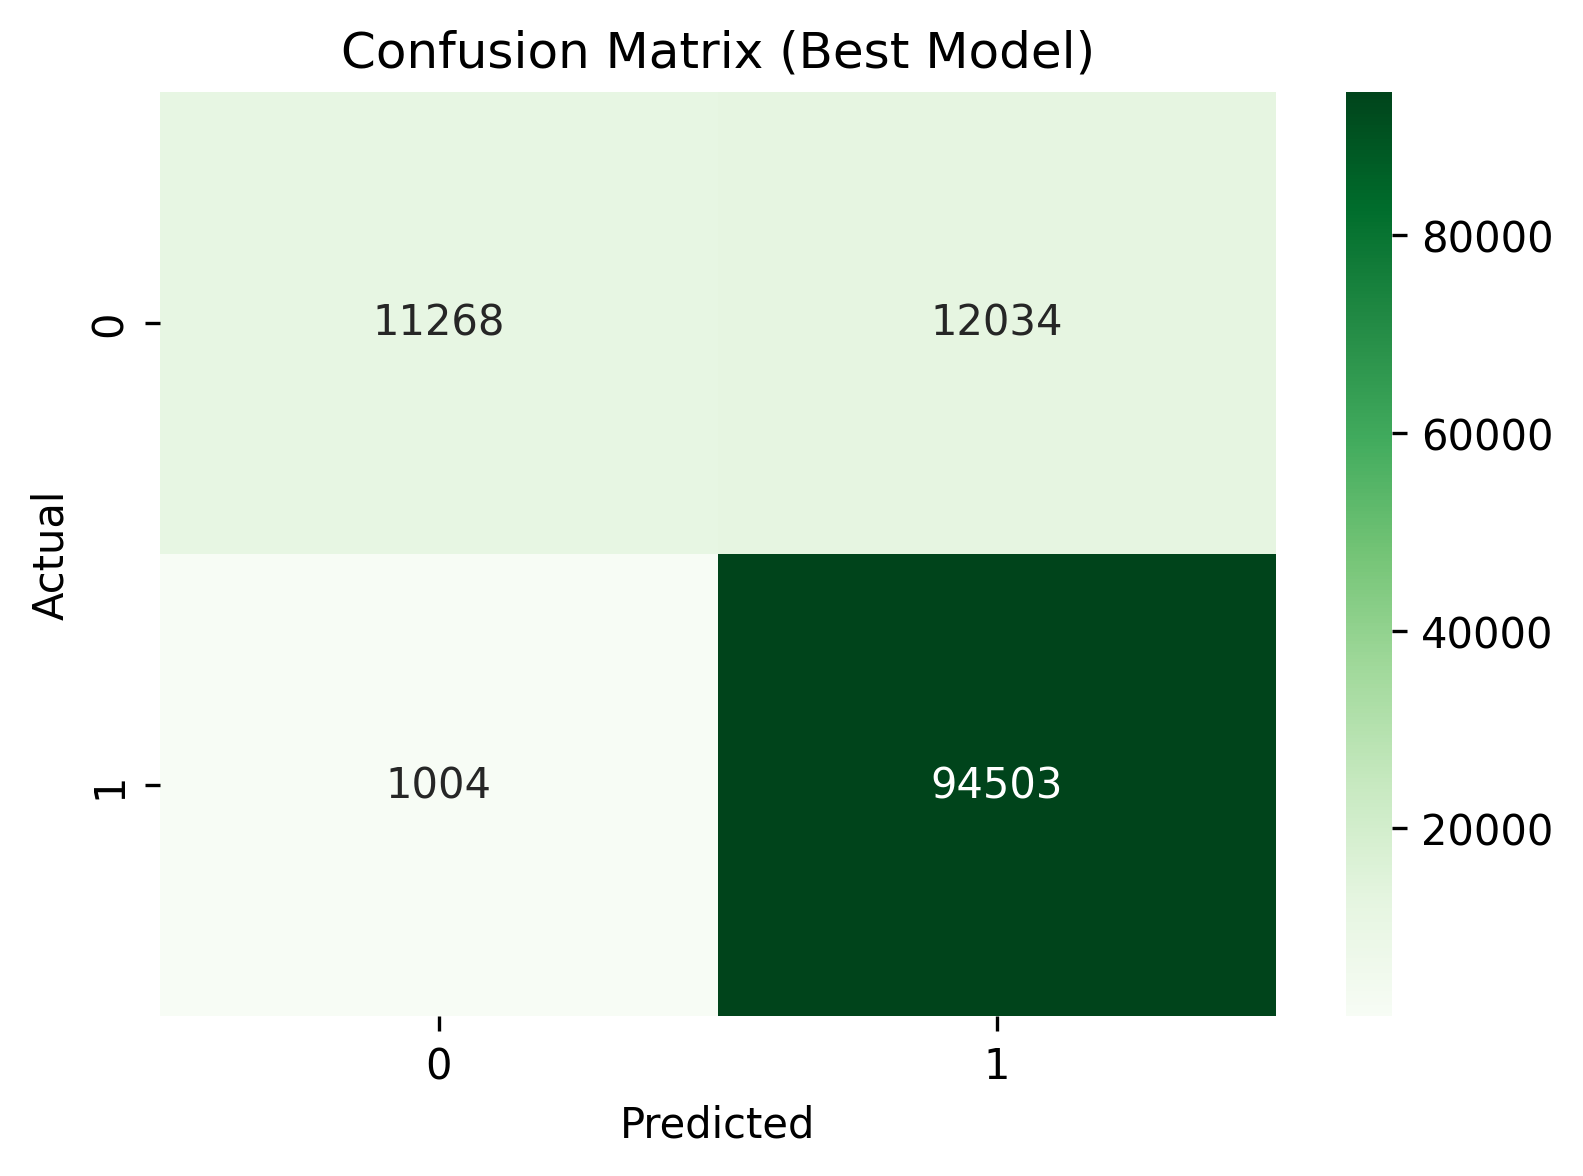
\includegraphics[width=0.8\textwidth,height=\textheight]{plots/confusion_matrix.png}

\subcaption{\label{}XGBoost Confusion Matrix}
\end{minipage}%
%
\begin{minipage}{0.50\linewidth}

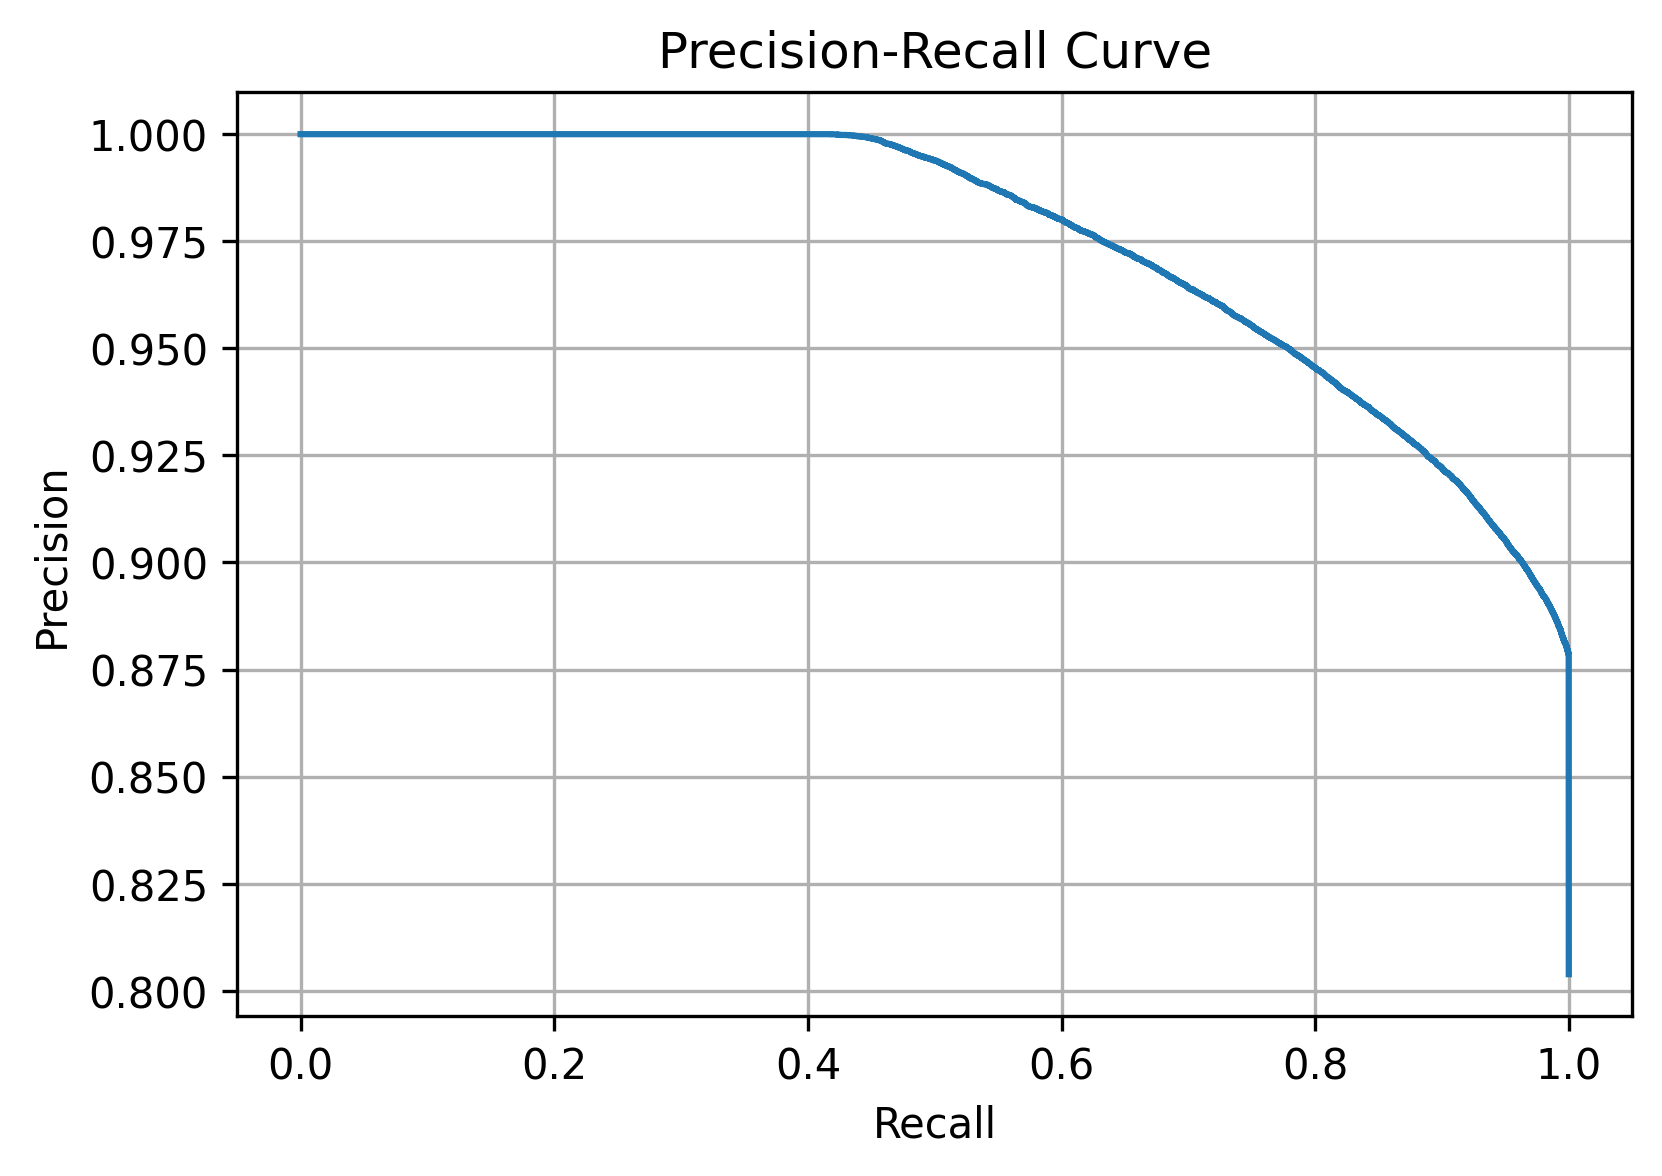
\includegraphics[width=0.8\textwidth,height=\textheight]{plots/precision_recall_curve.png}

\subcaption{\label{}XGBoost PRCurve}
\end{minipage}%

\end{figure}%

\newpage

\subsection*{변수 중요도(Feature Importance)
분석}\label{uxbcc0uxc218-uxc911uxc694uxb3c4feature-importance-uxbd84uxc11d}
\addcontentsline{toc}{subsection}{변수 중요도(Feature Importance) 분석}

\textbf{기본 변수 중요도} 산출 결과 부도 여부에는 예상 외로
\textbf{주거지가 큰 영향}을 미치는 것을 확인할 수 있었으며, 이외에도
\textbf{대출기간 등이 분류에 영향}을 미치는 것을 알 수 있었습니다.

\begin{center}
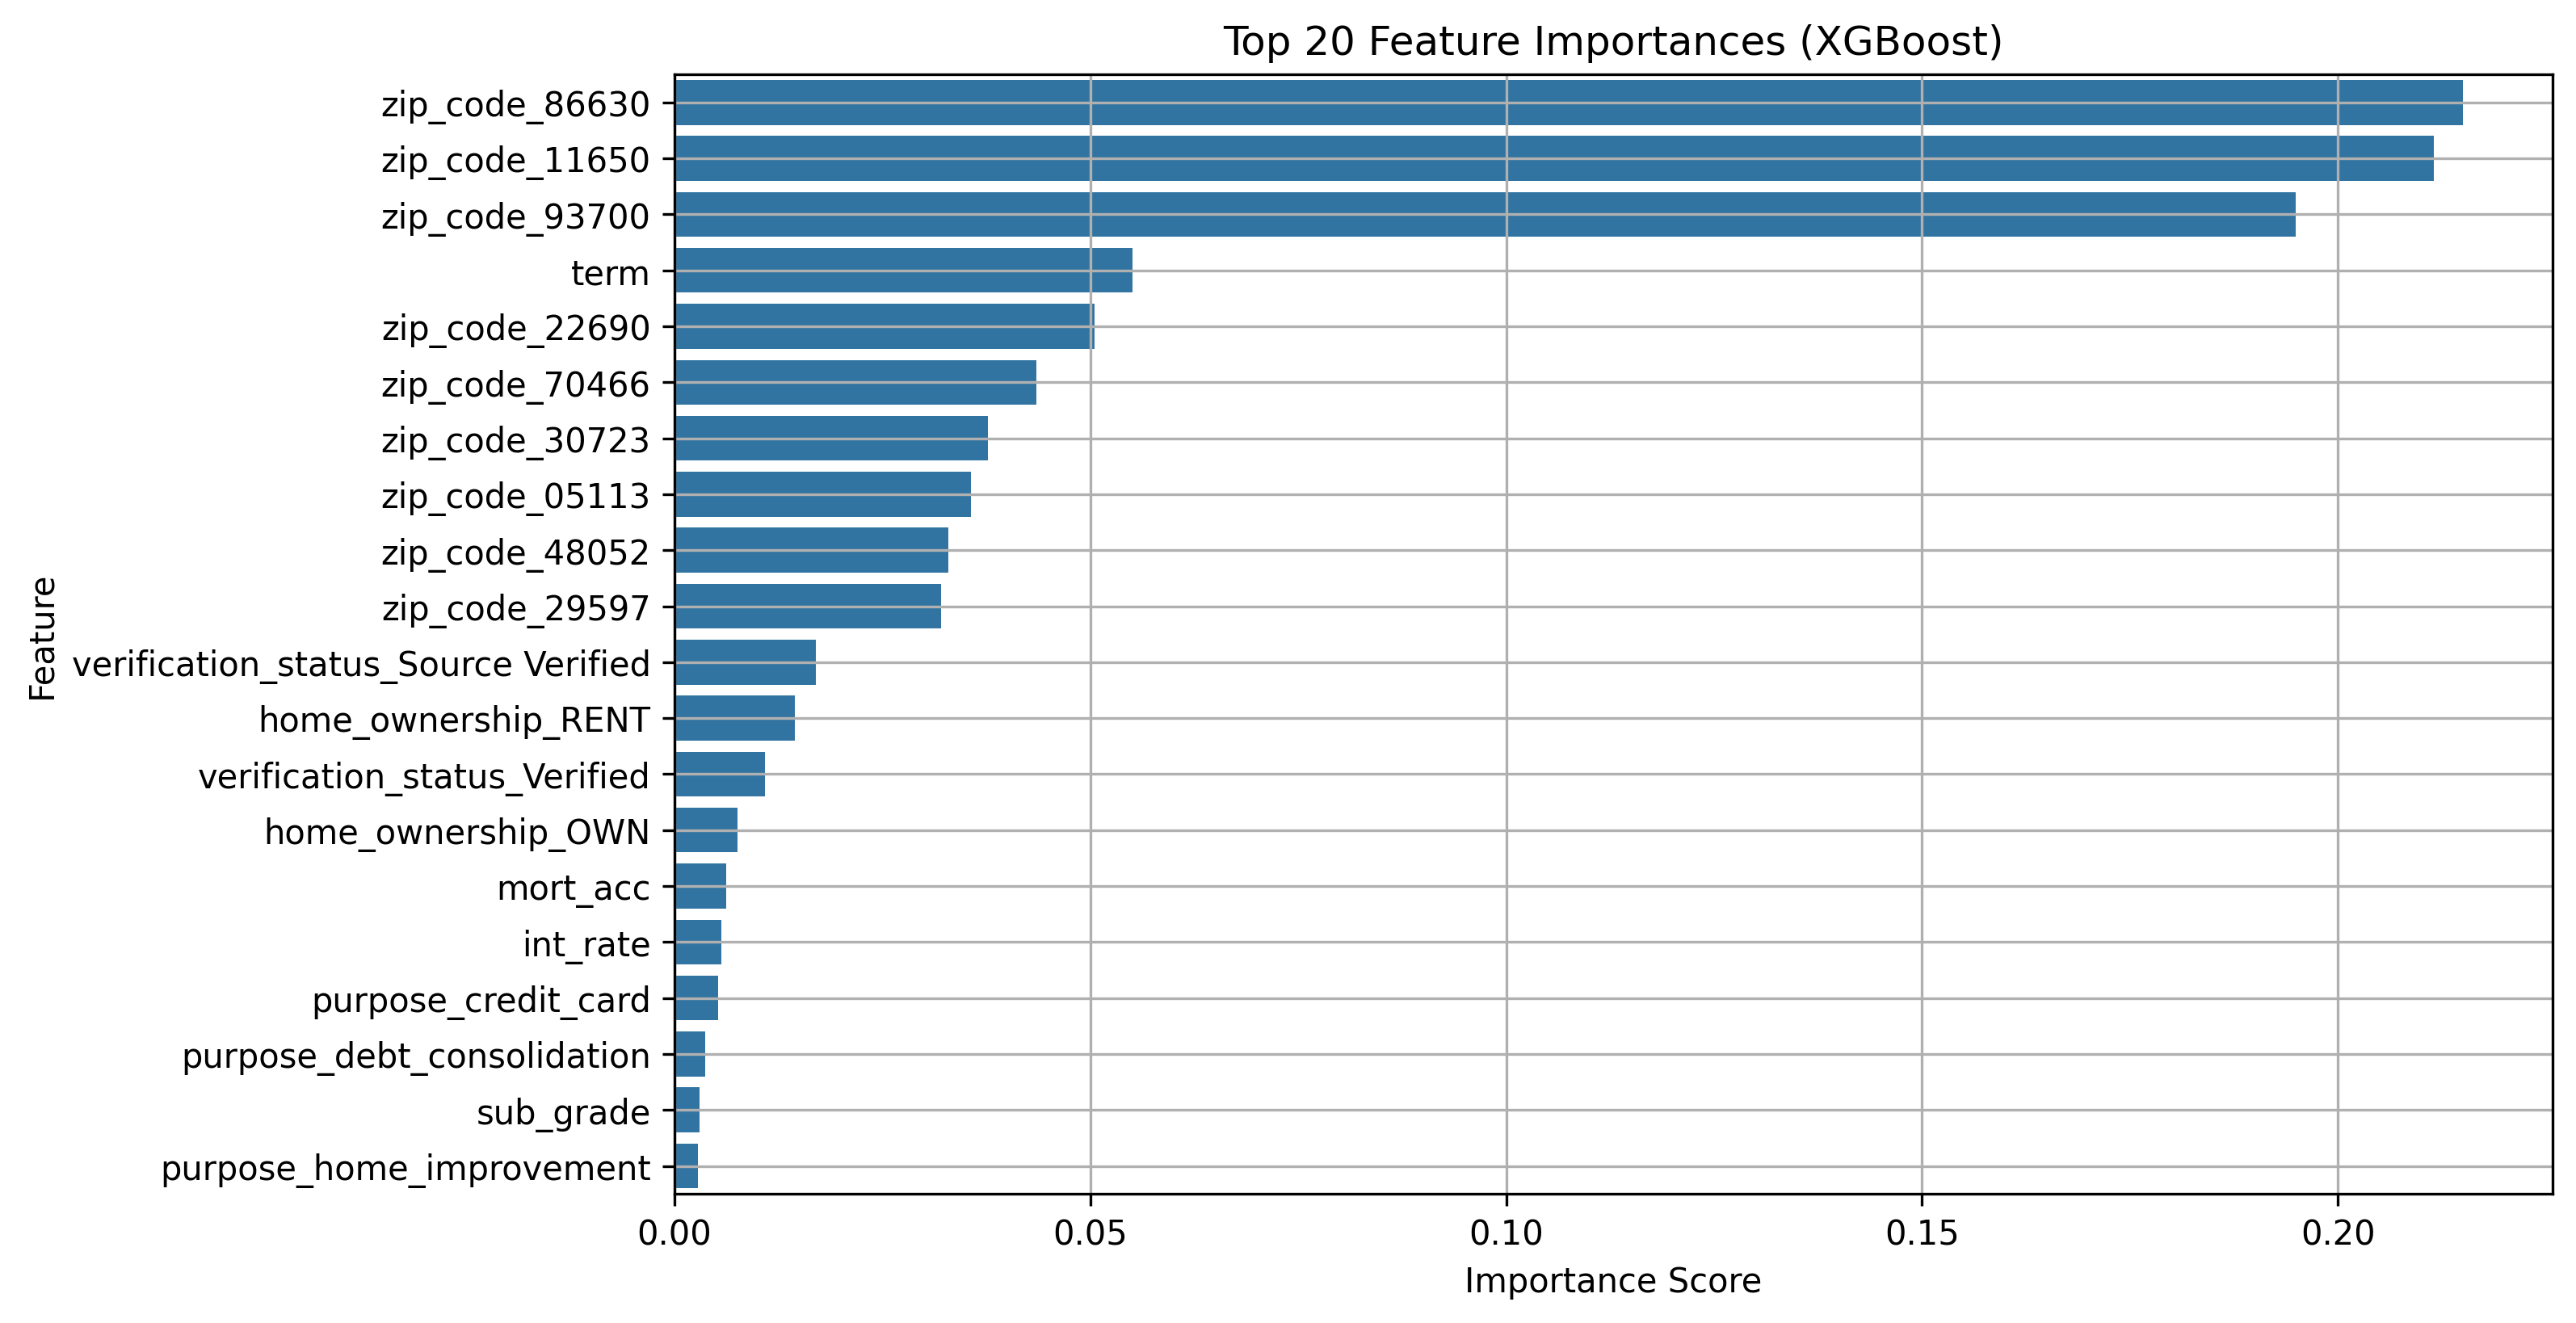
\includegraphics[width=0.65\textwidth,height=\textheight]{plots/feature_importance.png}
\end{center}

보다 \textbf{상세한 변수 중요도 분석을 위해 SHAP(SHapley Additive
exPlanations) 분석}을 실시하여 \textbf{각 변수의 중요도, 예측에 미치는
영향(방향성, 정도)을 분석}하였습니다.

\begin{center}
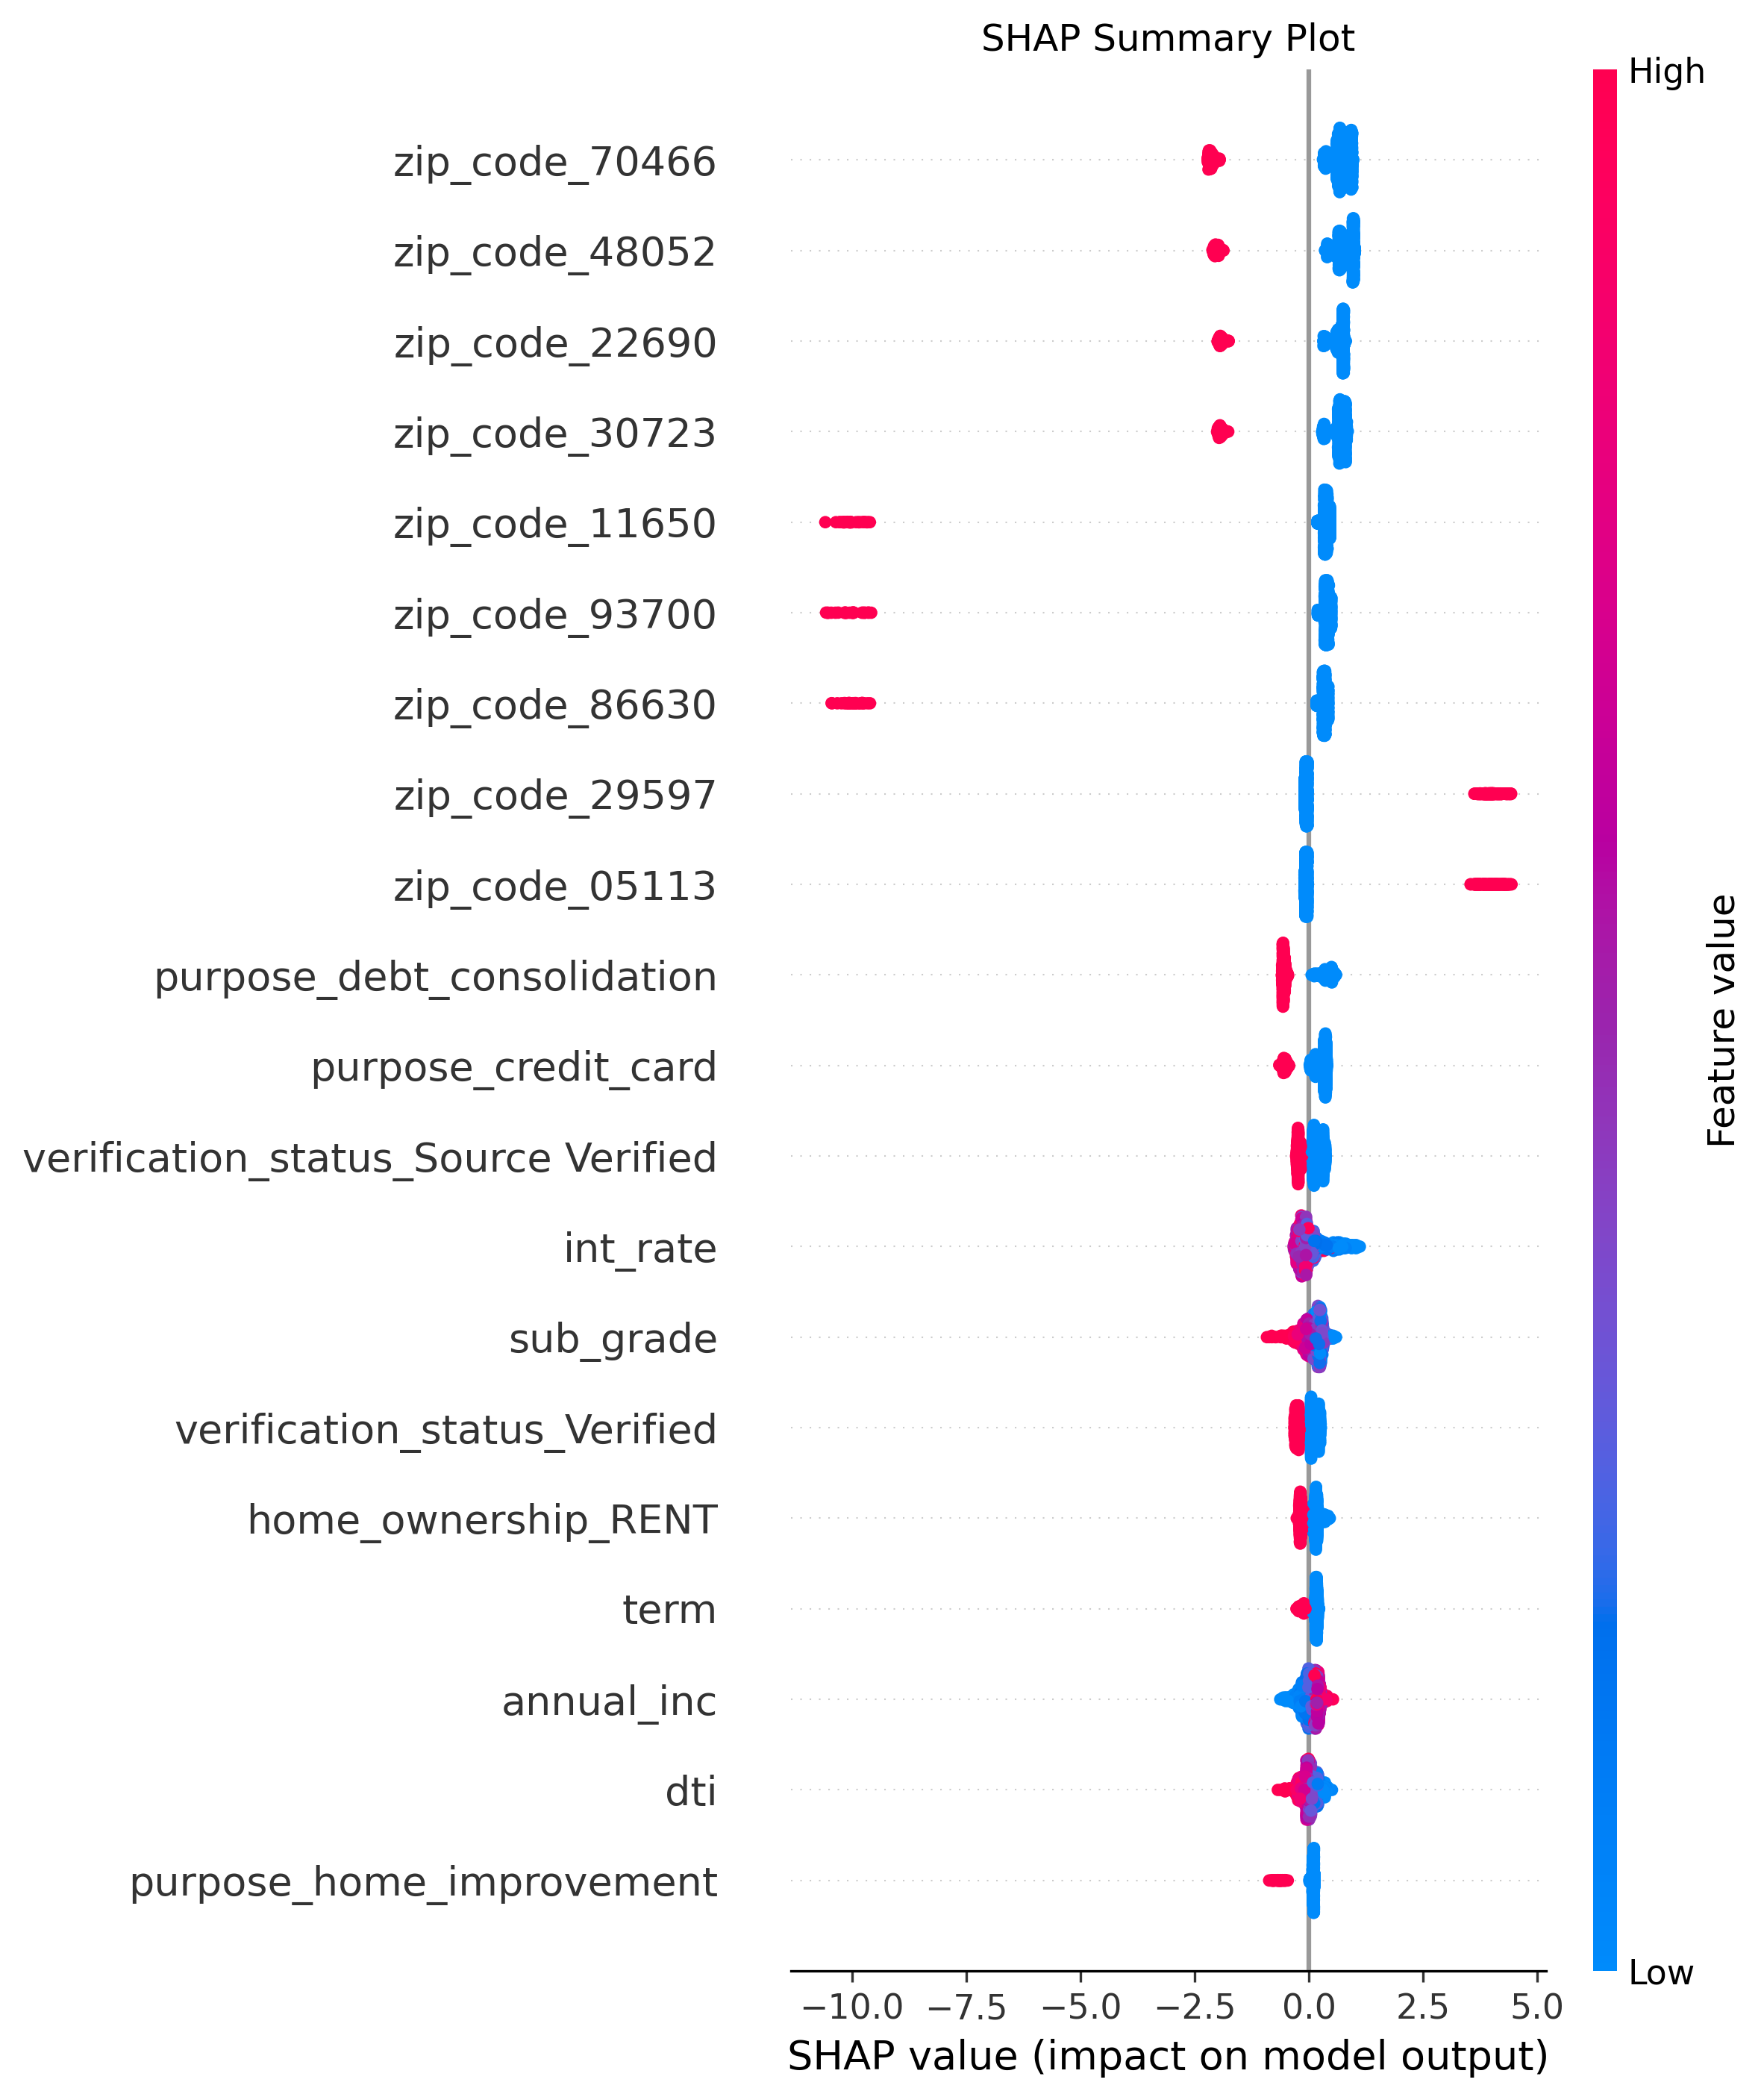
\includegraphics[width=0.65\textwidth,height=\textheight]{plots/shap_summary_plot.png}
\end{center}

\newpage

전체적인 중요도는 \textbf{주거지가 큰 영향을 미친다는 점에서
유사}하였으며, 변수별 특징은 아래와 같습니다.

\begin{verbatim}
-   상위 7개는 해당 지역에 주거(1) 시, 연체(0)가 많으므로 집값/소득수준이 낮은 주거지로 추정
-   하위 2개는 집값/소득수준이 높은 주거지로 추정
-   대출목적이 부채상환/신용카드, 대출이자가 높고, 대출기간이 길고, 소득이 낮을수록 연체 예측 가능성 증가
-   이 외에도 대부분의 변수가 대출과 관련된 일반적인 직관과 동일한 것을 알 수 있었음
\end{verbatim}

\subsection*{시사점}\label{uxc2dcuxc0acuxc810}
\addcontentsline{toc}{subsection}{시사점}

\textbf{이번 프로젝트를 통해 실제 은행의 데이터를 살펴보고, 대출의 부도
확률 예측 모델을 구축}해보았습니다.

먼저 \textbf{실제 데이터를 전처리}하는 과정에서 발생하는 결측치, 이상치,
적합하지 않은 변수 분류 등의 \textbf{문제점을 실제로 경험}할 수 있었고
Isolation Forest 및 T-SNE, Boruta 알고리즘을 적용해보면서 \textbf{각
알고리즘이 어떻게 작동하는지, 어떤 방식으로 문제를 해결하고 활용}되는지
알 수 있었습니다.

또한, \textbf{XGBoost 알고리즘}이 \textbf{금융데이터 예측에 강력한
성능}을 가진 것을 확인하였고, 모델 성능에는 알고리즘 선택 뿐만아니라
\textbf{하이퍼파라미터 튜닝 방법(2단계 최적화) 클래스 불균형
해소(oversampling), 변수 선별(boruta) 등이 매우 중요}하다는 것을
느꼈습니다.

결과적으로 은행 대출의 \textbf{연체여부에는 주거지가 매우 큰 영향}을
미친것으로 나타났으며, 이는 \textbf{주거지에
집값/주거형태/소득/신용점수/직업 등 종합적인 요소가 모두 반영}되어있기
때문인 것으로 추정됩니다. 이외에도 \textbf{이자율, 대출목적/기간 등이
연체 여부 예측에 영향}을 미치는 것으로 나타났으며, \textbf{그 영향은
일반적인 직관과 동일}하였습니다.

데이터 자체의 한계점으로 인해 소수 표본에 대한 학습이 부족하여 예측력이
다소 떨어지는 한계점이 있었으나, \textbf{전반적으로 수업시간에 다룬 여러
알고리즘을 통해 이론이 실제 세상에 적용되는 과정을 이해}할 수
있었습니다. 또한, \textbf{분석에 적합한 데이터를 구하고 전처리하는 것이
매우 중요}하다는 것을 알게 된 프로젝트였습니다.

\part{알고리즘 거래전략('25 봄)}

\chapter*{알고리즘 거래전략과 고빈도
금융}\label{uxc54cuxace0uxb9acuxc998-uxac70uxb798uxc804uxb7b5uxacfc-uxace0uxbe48uxb3c4-uxae08uxc735}
\addcontentsline{toc}{chapter}{알고리즘 거래전략과 고빈도 금융}

\markboth{알고리즘 거래전략과 고빈도 금융}{알고리즘 거래전략과 고빈도
금융}

\part{사례로 보는 금융공학('25 봄)}

\chapter*{사례로 보는 금융공학
실무}\label{uxc0acuxb840uxb85c-uxbcf4uxb294-uxae08uxc735uxacf5uxd559-uxc2e4uxbb34}
\addcontentsline{toc}{chapter}{사례로 보는 금융공학 실무}

\markboth{사례로 보는 금융공학 실무}{사례로 보는 금융공학 실무}

\chapter*{코스피200 변동성 조정 위클리 양매도
전략}\label{uxcf54uxc2a4uxd53c200-uxbcc0uxb3d9uxc131-uxc870uxc815-uxc704uxd074uxb9ac-uxc591uxb9e4uxb3c4-uxc804uxb7b5}
\addcontentsline{toc}{chapter}{코스피200 변동성 조정 위클리 양매도 전략}

\markboth{코스피200 변동성 조정 위클리 양매도 전략}{코스피200 변동성
조정 위클리 양매도 전략}

25년도 봄학기 금융공학 특수논제 A조

\textbf{김경재(20259048) / 강상묵(20259013) / 김형환(20249132) /
어환석(20259248) / 유수형(20259273)}

\section*{1. 개요}\label{uxac1cuxc694}
\addcontentsline{toc}{section}{1. 개요}

\markright{1. 개요}

본 리포트는 옵션과 변동성지수를 활용한 \textbf{변동성 조정 위클리
양매도}전략을 알아보고, \textbf{과거 데이터를 통해 구현 및 검증}하기
위해 작성되었습니다. \textbf{변동성 조정 위클리 양매도}란
\textbf{\emph{1.변동성 조정}}, \textbf{\emph{2.주단위 매도}} 두가지
특징을 통해 \textbf{기존 단점을 보완}한 양매도 전략으로, ``매주''
V-Kospi200를 이용해 행사가격 범위를 결정하고 콜/풋옵션을
매도(양매도)하게 됩니다.

전략 소개에 앞서 필요한 배경지식을 다루고, 전략 소개 및 구현, 백테스팅
및 성과를 차례로 설명하겠습니다.

\section*{2. 배경지식}\label{uxbc30uxacbduxc9c0uxc2dd}
\addcontentsline{toc}{section}{2. 배경지식}

\markright{2. 배경지식}

\subsection*{양매도 (Short
strangle)}\label{uxc591uxb9e4uxb3c4-short-strangle}
\addcontentsline{toc}{subsection}{양매도 (Short strangle)}

\textbf{양매도란 옵션 거래전략}으로, 일반적으로 \textbf{만기일이 같은
외가격(OTM) 콜/풋옵션을 매도}하는 것을 의미합니다.

OTM 옵션을 매도하므로, 만기일에 기초자산의 가격이 풋옵션의 행사가격과
콜옵션의 행사가격 사이라면 권리행사되지 않게 되고 \textbf{옵션
프리미엄(매도수익)을 그대로 얻을 수 있게 됩니다.}

반면, \textbf{양매도는 시장의 변동성이 예상과 달리 큰 경우, 큰 손실이
발생할 수 있다는 단점}도 존재합니다. \textbf{수익은 프리미엄으로
한정}되어있으나, 시황 급변에 따른 \textbf{옵션 손실에는 제한이 없어}
원금 이상의 손실이 발생할 수도 있기 때문입니다.

즉, 양매도는 높은 확률로 \textbf{안정적인 중수익을 보장하나 매우 낮은
확률로 큰 손실이 발생할 수 있는 전략}이며, \textbf{향후 시장의 변동성이
크지 않을 것이라 예측될 때 주로 사용}됩니다.

\begin{center}
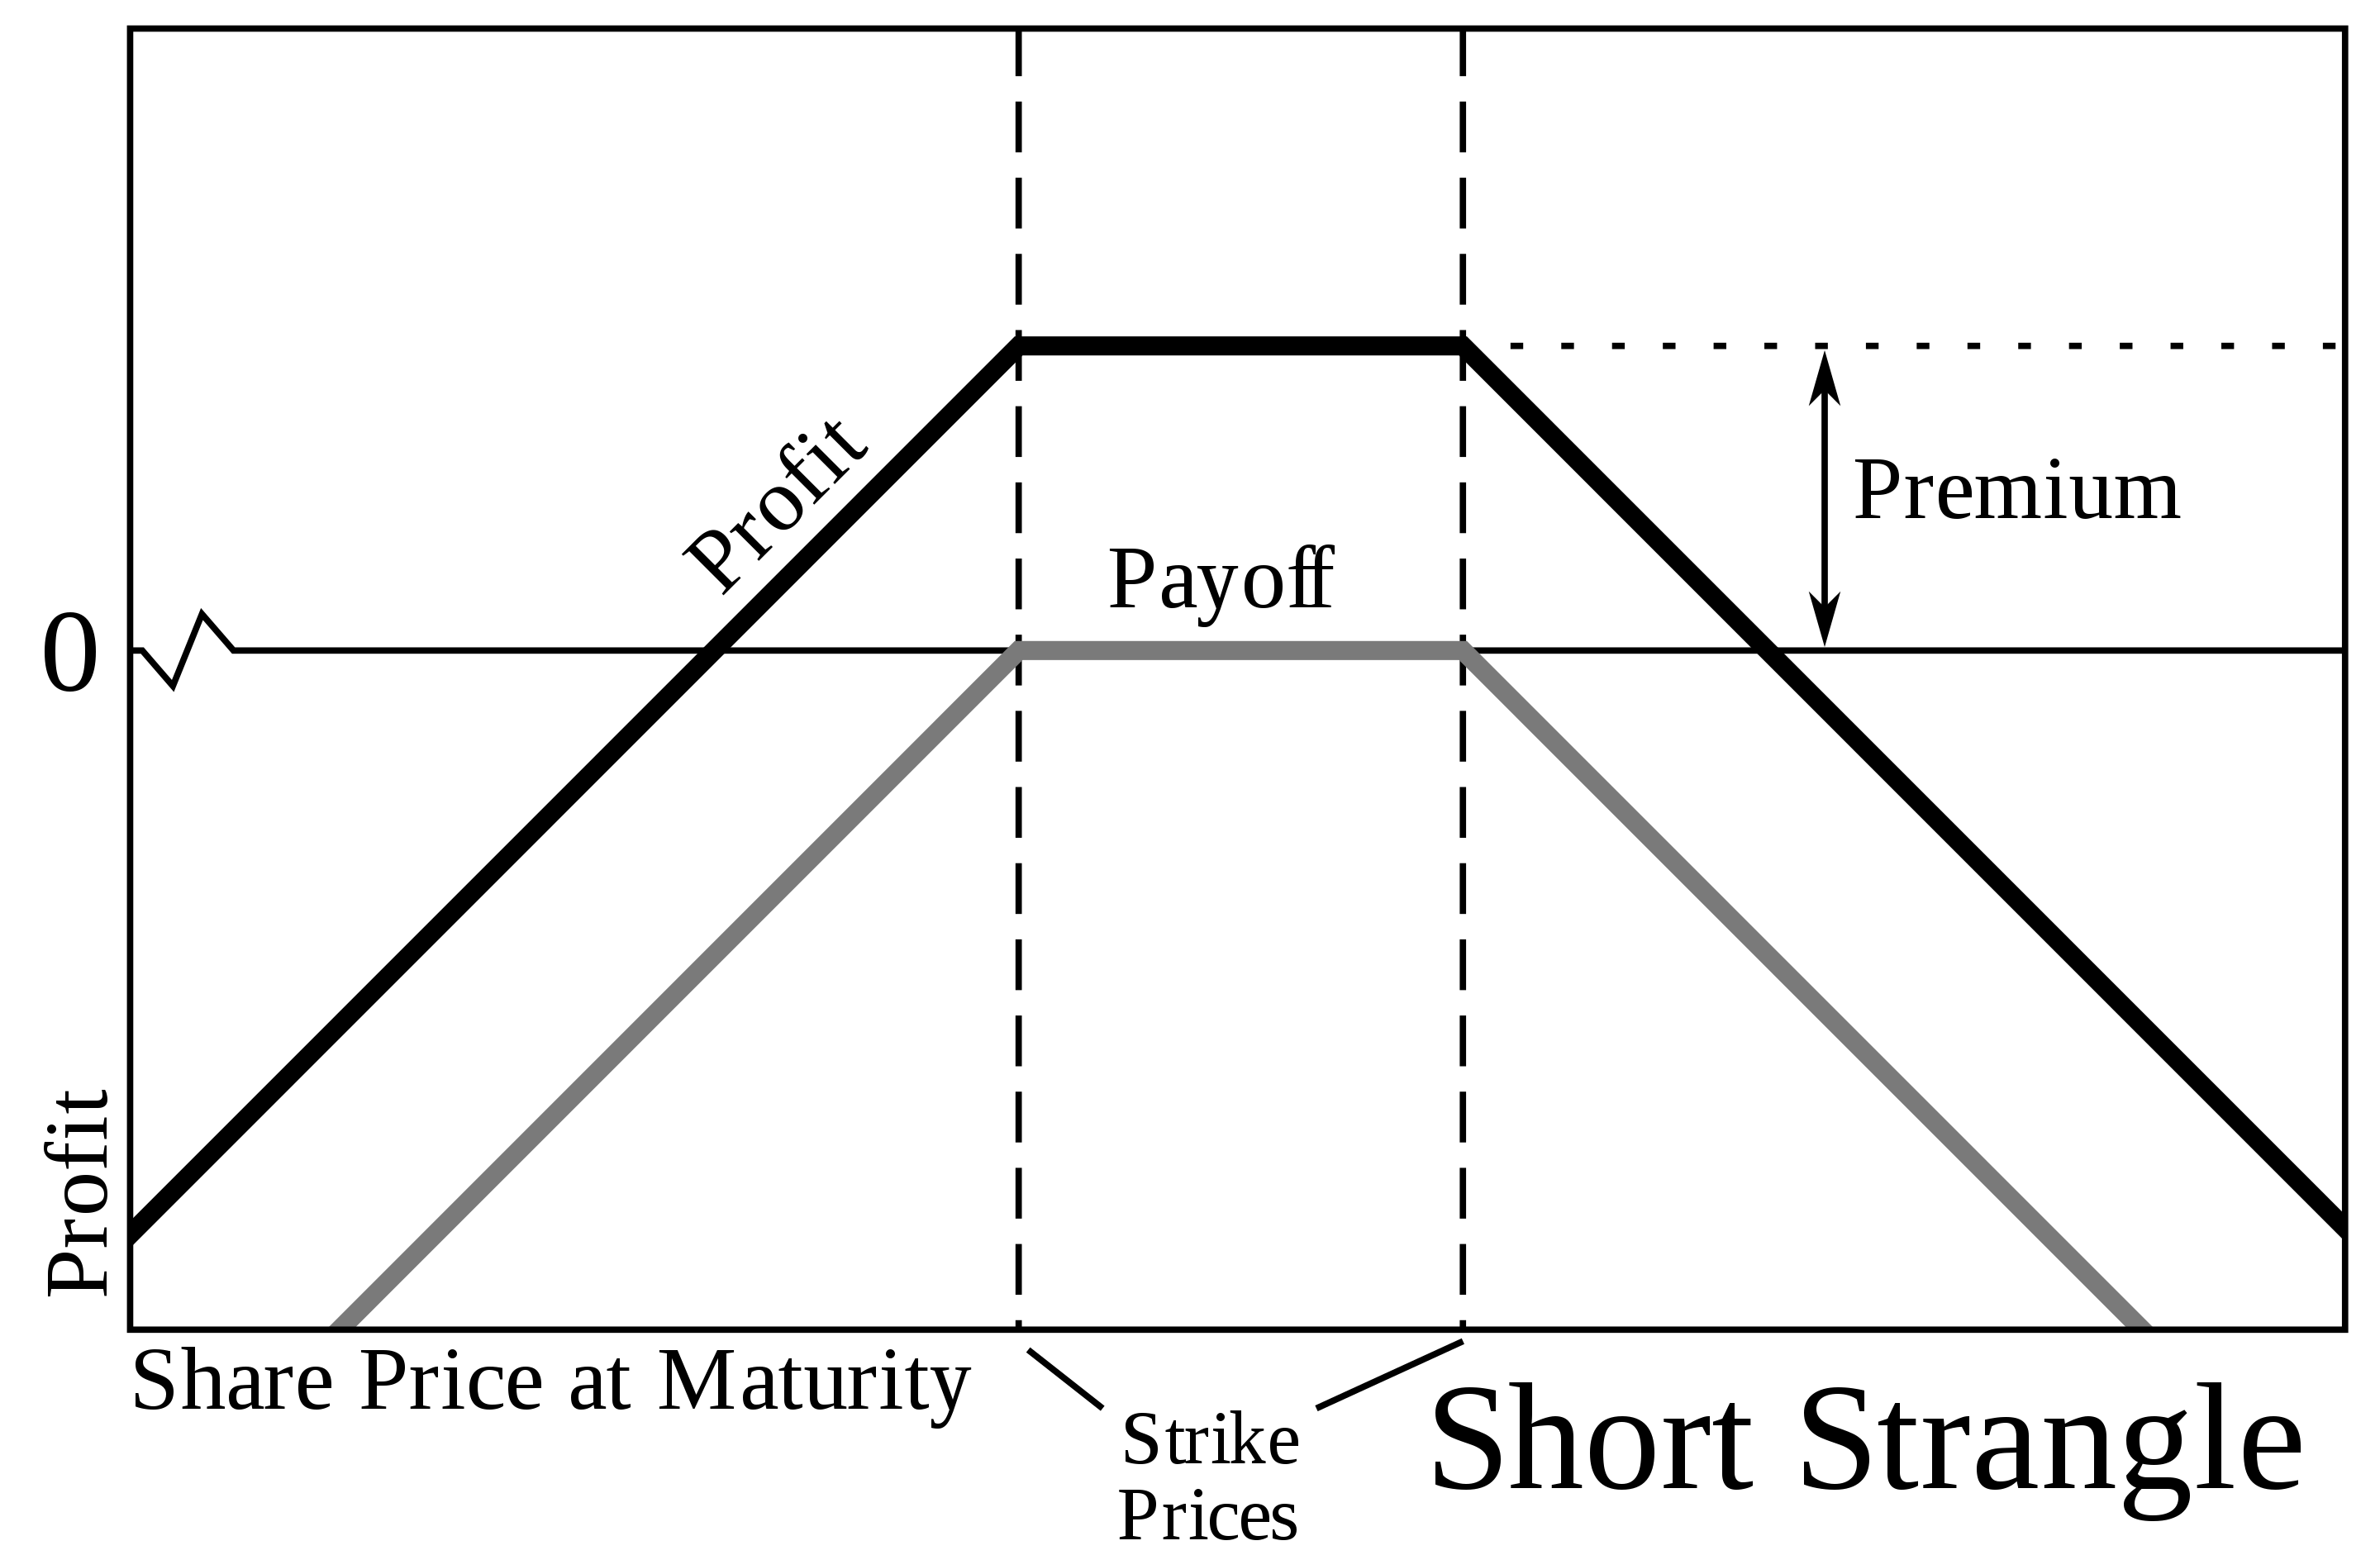
\includegraphics[width=150mm,height=50mm]{image/shortstrangle.png}
\end{center}

\subsubsection*{양매도 전략
예시}\label{uxc591uxb9e4uxb3c4-uxc804uxb7b5-uxc608uxc2dc}
\addcontentsline{toc}{subsubsection}{양매도 전략 예시}

국내의 경우 행사가격의 상하단을 등가격(ATM) \(\pm\) 5\%로 설정한 양매도
ETN이 한 때 큰 인기를 끌었습니다. 대표적인 예시인 \textbf{월별 코스피200
OTM 5\% 양매도 전략}의 거래방법을 살펴보면, 다음과 같습니다.

\begin{enumerate}
\def\labelenumi{\arabic{enumi}.}
\tightlist
\item
  현재 코스피200지수를 기준으로 ATM+5\%의 콜옵션과 ATM-5\%의 풋옵션을
  매도 (프리미엄 수익 발생)
\item
  다음달 만기일이 되면, 옵션은 청산(권리행사시 손실)되고 다시 ATM
  \(\pm\) 5\%의 콜,풋옵션을 매도
\end{enumerate}

즉, \textbf{월단위로 옵션을 교체하게 되며 행사가격의 상하단은 ATM}
\(\pm\) 5\%로 고정한 양매도 전략입니다. 중위험-중수익으로 흥행에 성공한
상품이지만, \textbf{아래와 같은 한계점}도 존재합니다.

\begin{enumerate}
\def\labelenumi{\arabic{enumi}.}
\tightlist
\item
  행사가격 범위가 고정되어있어 변동성 확대시 손실 가능성이 커지고,
  변동성 축소시 프리미엄 수익이 크게 감소
\item
  옵션 교체주기가 1개월로, 그간 지수의 하락이 누적된다면 손실이 과도하게
  커질 수 있음 (유동성 리스크)
\end{enumerate}

\subsection*{코스피200 변동성지수 (V-Kospi200
index)}\label{uxcf54uxc2a4uxd53c200-uxbcc0uxb3d9uxc131uxc9c0uxc218-v-kospi200-index}
\addcontentsline{toc}{subsection}{코스피200 변동성지수 (V-Kospi200
index)}

\textbf{코스피200 변동성 지수}란 주식 시장의 \textbf{변동성을 측정하는
지표}입니다. 코스피200 옵션 가격 기반의 내재변동성을 이용하여 산출되며,
향후 30일간 시장 변동성에 대한 투자자들의 기대를 나타내는 지수입니다.

\subsubsection*{주요 특징}\label{uxc8fcuxc694-uxd2b9uxc9d5}
\addcontentsline{toc}{subsubsection}{주요 특징}

\begin{itemize}
\tightlist
\item
  \textbf{시장 심리 반영}: 투자자들의 불안 심리를 반영하며, '공포
  지수(Fear Index)'라고도 불림
\item
  \textbf{옵션 가격 기반}: 코스피200 옵션 가격 기반의 내재변동성을 통해
  산출되며, 여기에는 투자자들의 기대가 반영
\end{itemize}

\textbf{\emph{그래프1 : 일별 코스피200지수 및 코스피200 변동성지수}}

\begin{center}
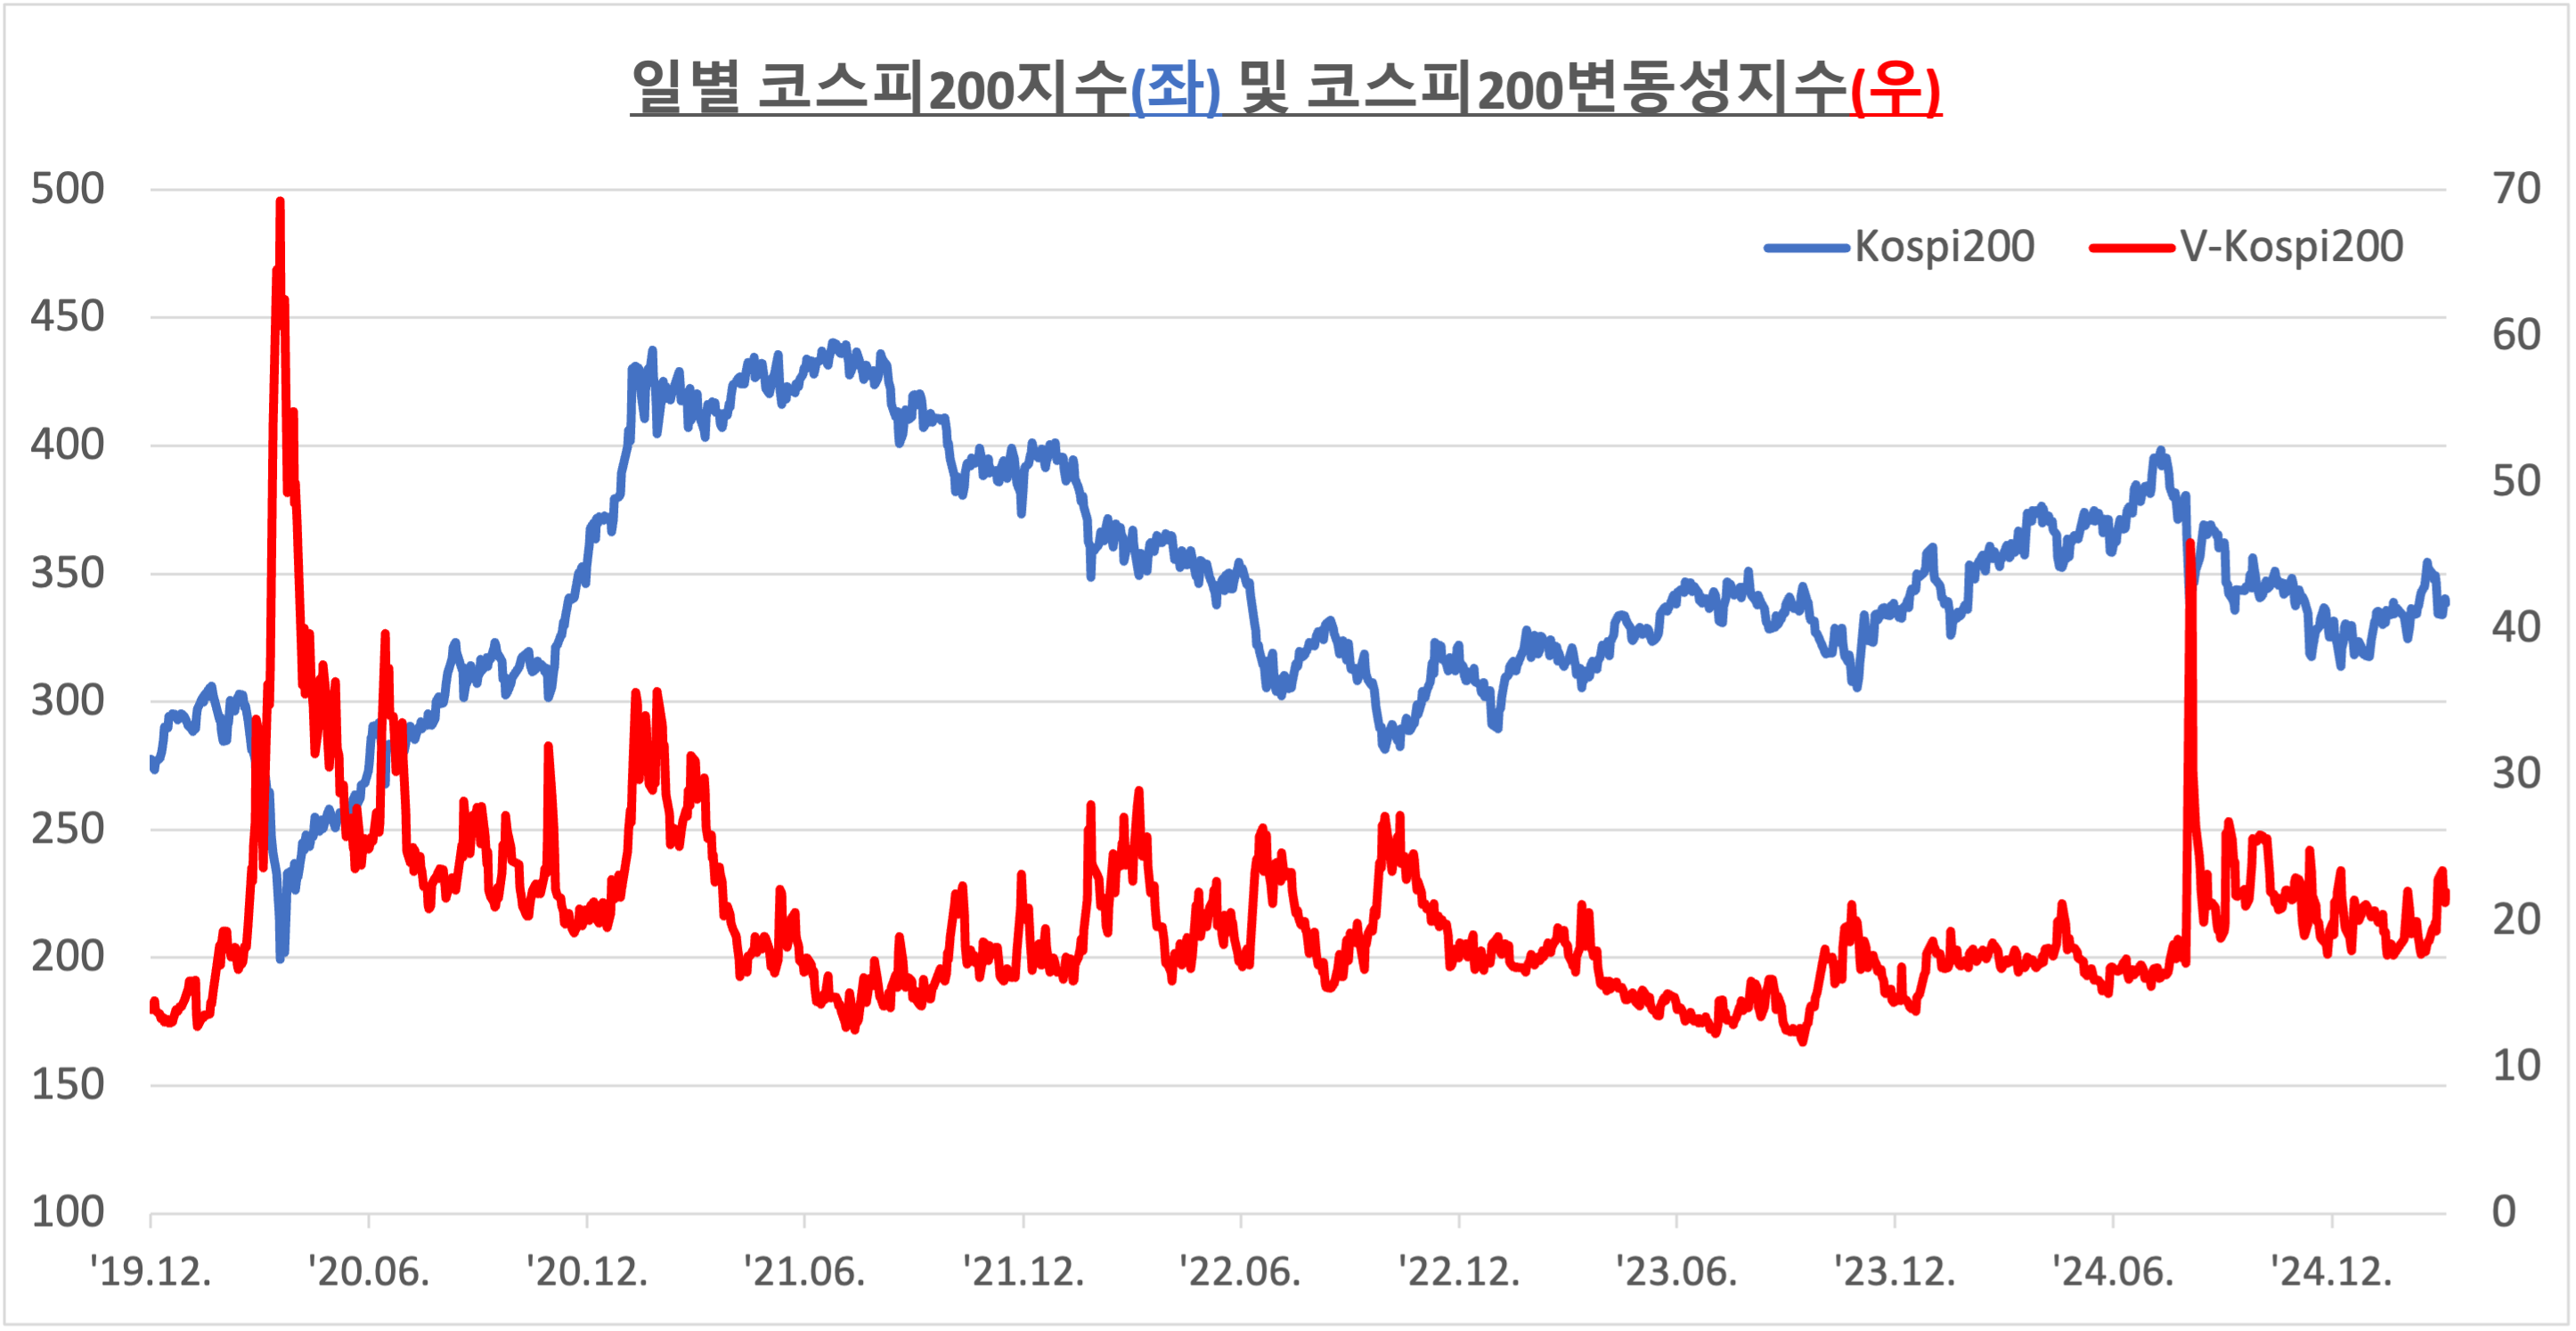
\includegraphics[width=0.7\textwidth,height=\textheight]{image/vkospi.png}
\end{center}

\subsection*{코스피200
위클리옵션}\label{uxcf54uxc2a4uxd53c200-uxc704uxd074uxb9acuxc635uxc158}
\addcontentsline{toc}{subsection}{코스피200 위클리옵션}

\textbf{코스피200 위클리옵션}이란 코스피200 지수를 기초자산으로 하는
\textbf{주간 단위의 옵션 거래 상품}을 말합니다. '19년 상장되었으며
기존의 월 단위 만기가 도래하는 옵션과는 달리, 매주 월/목요일에 만기가
도래하는 단기 옵션입니다.

\subsubsection*{주요 특징}\label{uxc8fcuxc694-uxd2b9uxc9d5-1}
\addcontentsline{toc}{subsubsection}{주요 특징}

\begin{itemize}
\tightlist
\item
  \textbf{세밀한 거래 지원}: 매주 월/목요일에 만기가 도래하여 단기적인
  시장 변동에 대한 투자 및 위험 관리에 유리
\item
  \textbf{다양한 투자 전략 활용:} 단기적인 시장 예측을 기반으로 다양한
  투자 전략을 구사할 수 있습니다.
\end{itemize}

\section*{3. 전략 소개 및
구현}\label{uxc804uxb7b5-uxc18cuxac1c-uxbc0f-uxad6cuxd604}
\addcontentsline{toc}{section}{3. 전략 소개 및 구현}

\markright{3. 전략 소개 및 구현}

\subsection*{전략 개요}\label{uxc804uxb7b5-uxac1cuxc694}
\addcontentsline{toc}{subsection}{전략 개요}

변동성 조정 위클리 양매도(Volatility Adjusted Weekly Short strangle,
VWss) 전략이란, 기존에 널리 활용되던 \textbf{월별 OTM 5\% 양매도 전략}에
아래 두가지 방법을 결합한 전략을 의미합니다.

\begin{enumerate}
\def\labelenumi{\arabic{enumi}.}
\tightlist
\item
  옵션의 교체주기를 ``매월'' -\textgreater{} ``매주'' 단위로 세분화
\item
  행사가격의 범위를 고정하는 것이 아니라 매 옵션 매도시점마다 시장
  변동성을 고려하여 조정
\end{enumerate}

따라서, 기존과 달리 \textbf{주단위로 옵션을 교체하며, 행사가격의 범위는
교체시점에 매번 달라지게 됩니다.} 이를 위해
코스피200위클리옵션\textbf{을 사용하고, 변동성 지표는} 내재변동성 기반의
V-Kospi200지수를 사용**하여 구현할 계획입니다.

\subsection*{행사가격 범위
설정방법}\label{uxd589uxc0acuxac00uxaca9-uxbc94uxc704-uxc124uxc815uxbc29uxbc95}
\addcontentsline{toc}{subsection}{행사가격 범위 설정방법}

행사가격의 상하단은 \textbf{옵션 매도시점의 ``전일 V-Kospi200 종가''를
참조하여 설정}할 예정입니다. V-Kospi200는 향후 30일간 코스피200 지수의
변동성을 수치화한 지표로서, 현재시점에서 변동성을 잘 예측할 수 있는
수단이기 때문입니다.

다만, 본 전략에서 옵션 매도포지션의 유지기간은 약 7일이므로 지수
종가(연율)를 주단위 기간에 맞도록 환산하여 행사가격의 상하단을
산출하였습니다.

\[\sigma_{Target}\;=\;\frac{VKospi200_{(T-1)}\times\sqrt{Calendar\;days}}{\sqrt{365}}\]

\[Call\;strike\;=\;Kospi200_{(T)}\times (1+\sigma_{Target})\;rounded\;up\;to\;2.5pt\]

\[Put\;strike\;=\;Kospi200_{(T)}\times (1-\sigma_{Target})\;rounded\;down\;to\;2.5pt\]

이렇게 행사가격을 설정하면 V-Kospi200가 15pt일 때 월환산 변동성이 약
5\%(주환산 2.5\%)가 됩니다. 즉,

\begin{itemize}
\tightlist
\item
  시장의 예상 변동성(V-Kospi200)이 연 15\% 이상 -\textgreater{} 행사가격
  범위를 기존보다 넓게 설정하여 손실 가능성 축소
\item
  시장의 예상 변동성이 연 15\% 미만 -\textgreater{} 행사가격 범위를
  기존보다 좁게 설정하여 프리미엄 수익 극대화
\end{itemize}

\begin{tcolorbox}[enhanced jigsaw, breakable, colframe=quarto-callout-color-frame, bottomrule=.15mm, arc=.35mm, opacityback=0, leftrule=.75mm, left=2mm, toprule=.15mm, rightrule=.15mm, colback=white]

본 전략은 위클리옵션을 사용하므로 향후 1주일 변동성이 필요합니다.
따라서, 30일 변동성을 나타내는 V-Kospi200은 만기 mismatch가 있지만,
단기간의 예측치에는 큰 차이가 없고 이외의 대안(e.g.~7-day VIX)이 없어
V-Kospi200를 그대로 사용하였습니다.

\end{tcolorbox}

\subsection*{포트폴리오 구성
방법}\label{uxd3ecuxd2b8uxd3f4uxb9acuxc624-uxad6cuxc131-uxbc29uxbc95}
\addcontentsline{toc}{subsection}{포트폴리오 구성 방법}

먼저, 편의를 위해 세금/수수료/호가스프레드 등의 거래비용은 없으며 종가에
원하는 수량만큼 거래할 수 있는 \textbf{완전자본시장을 가정}하도록
하겠습니다. 전략 구현을 위한 포트폴리오(투자원금 100억원) 구성 과정은
아래와 같습니다.

\begin{enumerate}
\def\labelenumi{\arabic{enumi}.}
\tightlist
\item
  전일 V-Kospi200 지수를 주단위로 환산하여
  예상변동성(\(\hat\sigma=(VKospi200\times \sqrt{day})/\sqrt{365}\))
  산출
\item
  예상변동성을 당일 Kospi200지수에 적용하여 행사가격 상하단(ATM
  \(\pm\hat\sigma\)을 2.5pt 단위로 올림/내림) 산출
\item
  당일 Kospi200지수 및 승수(25만)를 적용, 옵션
  매도수량(\(Q_{sell}=nominal/(kospi200\times multiplier)\)) 산출
\item
  행사가격 상단 콜옵션, 하단 풋옵션 매도
  (\(Premium=(call price+put price)\times Q_{sell}\times multiplier\))
\item
  원금과 매도수익을 다음주 만기일까지 MMF에 투자
  (\(Interest=(nominal+Premium)\times MMF \times \frac{day}{365}\))
\item
  다음주 만기일이 되면, 권리행사 손실을 포함하여 최종손익
  산출(\(Revenue=Premium+Interest-Exercise\))

  \begin{itemize}
  \tightlist
  \item
    Kospi200 \textgreater{} 행사가격 상단, 콜옵션에서 손실
    발생(\(Exercise=(Kospi200-Strike_{call})\times multiplier\))
  \item
    Kospi200 \textless{} 행사가격 하단, 풋옵션에서 손실
    발생(\(Exercise=(Strike_{put}-Kospi200)\times multiplier\))
  \item
    이외의 경우, 권리행사되지 않아 옵션 포지션 청산(\(Exercise=0\))
  \end{itemize}
\item
  주간 최종손익을 정산(\(nominal_{new}=nominal_{old}+Revenue\))하고,
  투자종료시점까지 1. \textasciitilde{} 6. 과정을 반복
\end{enumerate}

\section*{3. Backtesting}\label{backtesting}
\addcontentsline{toc}{section}{3. Backtesting}

\markright{3. Backtesting}

\subsection*{데이터 수집 및 전처리, 포트폴리오
구현}\label{uxb370uxc774uxd130-uxc218uxc9d1-uxbc0f-uxc804uxcc98uxb9ac-uxd3ecuxd2b8uxd3f4uxb9acuxc624-uxad6cuxd604}
\addcontentsline{toc}{subsection}{데이터 수집 및 전처리, 포트폴리오
구현}

과거 5개년(2020\textasciitilde2024) 코스피200 등의 지수/옵션 가격,
금리를 수집하였으며, 출처는 아래와 같습니다.

\begin{verbatim}
한국거래소 정보데이터시스템(data.krx.co.kr) : 코스피200 및 V-Kospi200지수
한국거래소 OpenAPI(openapi.krx.co.kr) : 코스피200옵션 및 위클리옵션 종목별 가격
한국은행 경제통계시스템(ecos.bok.or.kr) : 일별 MMF(7일) 금리
\end{verbatim}

\begin{tcolorbox}[enhanced jigsaw, bottomtitle=1mm, breakable, coltitle=black, opacityback=0, titlerule=0mm, left=2mm, colbacktitle=quarto-callout-note-color!10!white, toptitle=1mm, colframe=quarto-callout-note-color-frame, bottomrule=.15mm, opacitybacktitle=0.6, leftrule=.75mm, title=\textcolor{quarto-callout-note-color}{\faInfo}\hspace{0.5em}{한국거래소 OpenAPI를 활용한 데이터 수집 예시}, arc=.35mm, toprule=.15mm, rightrule=.15mm, colback=white]

\begin{center}
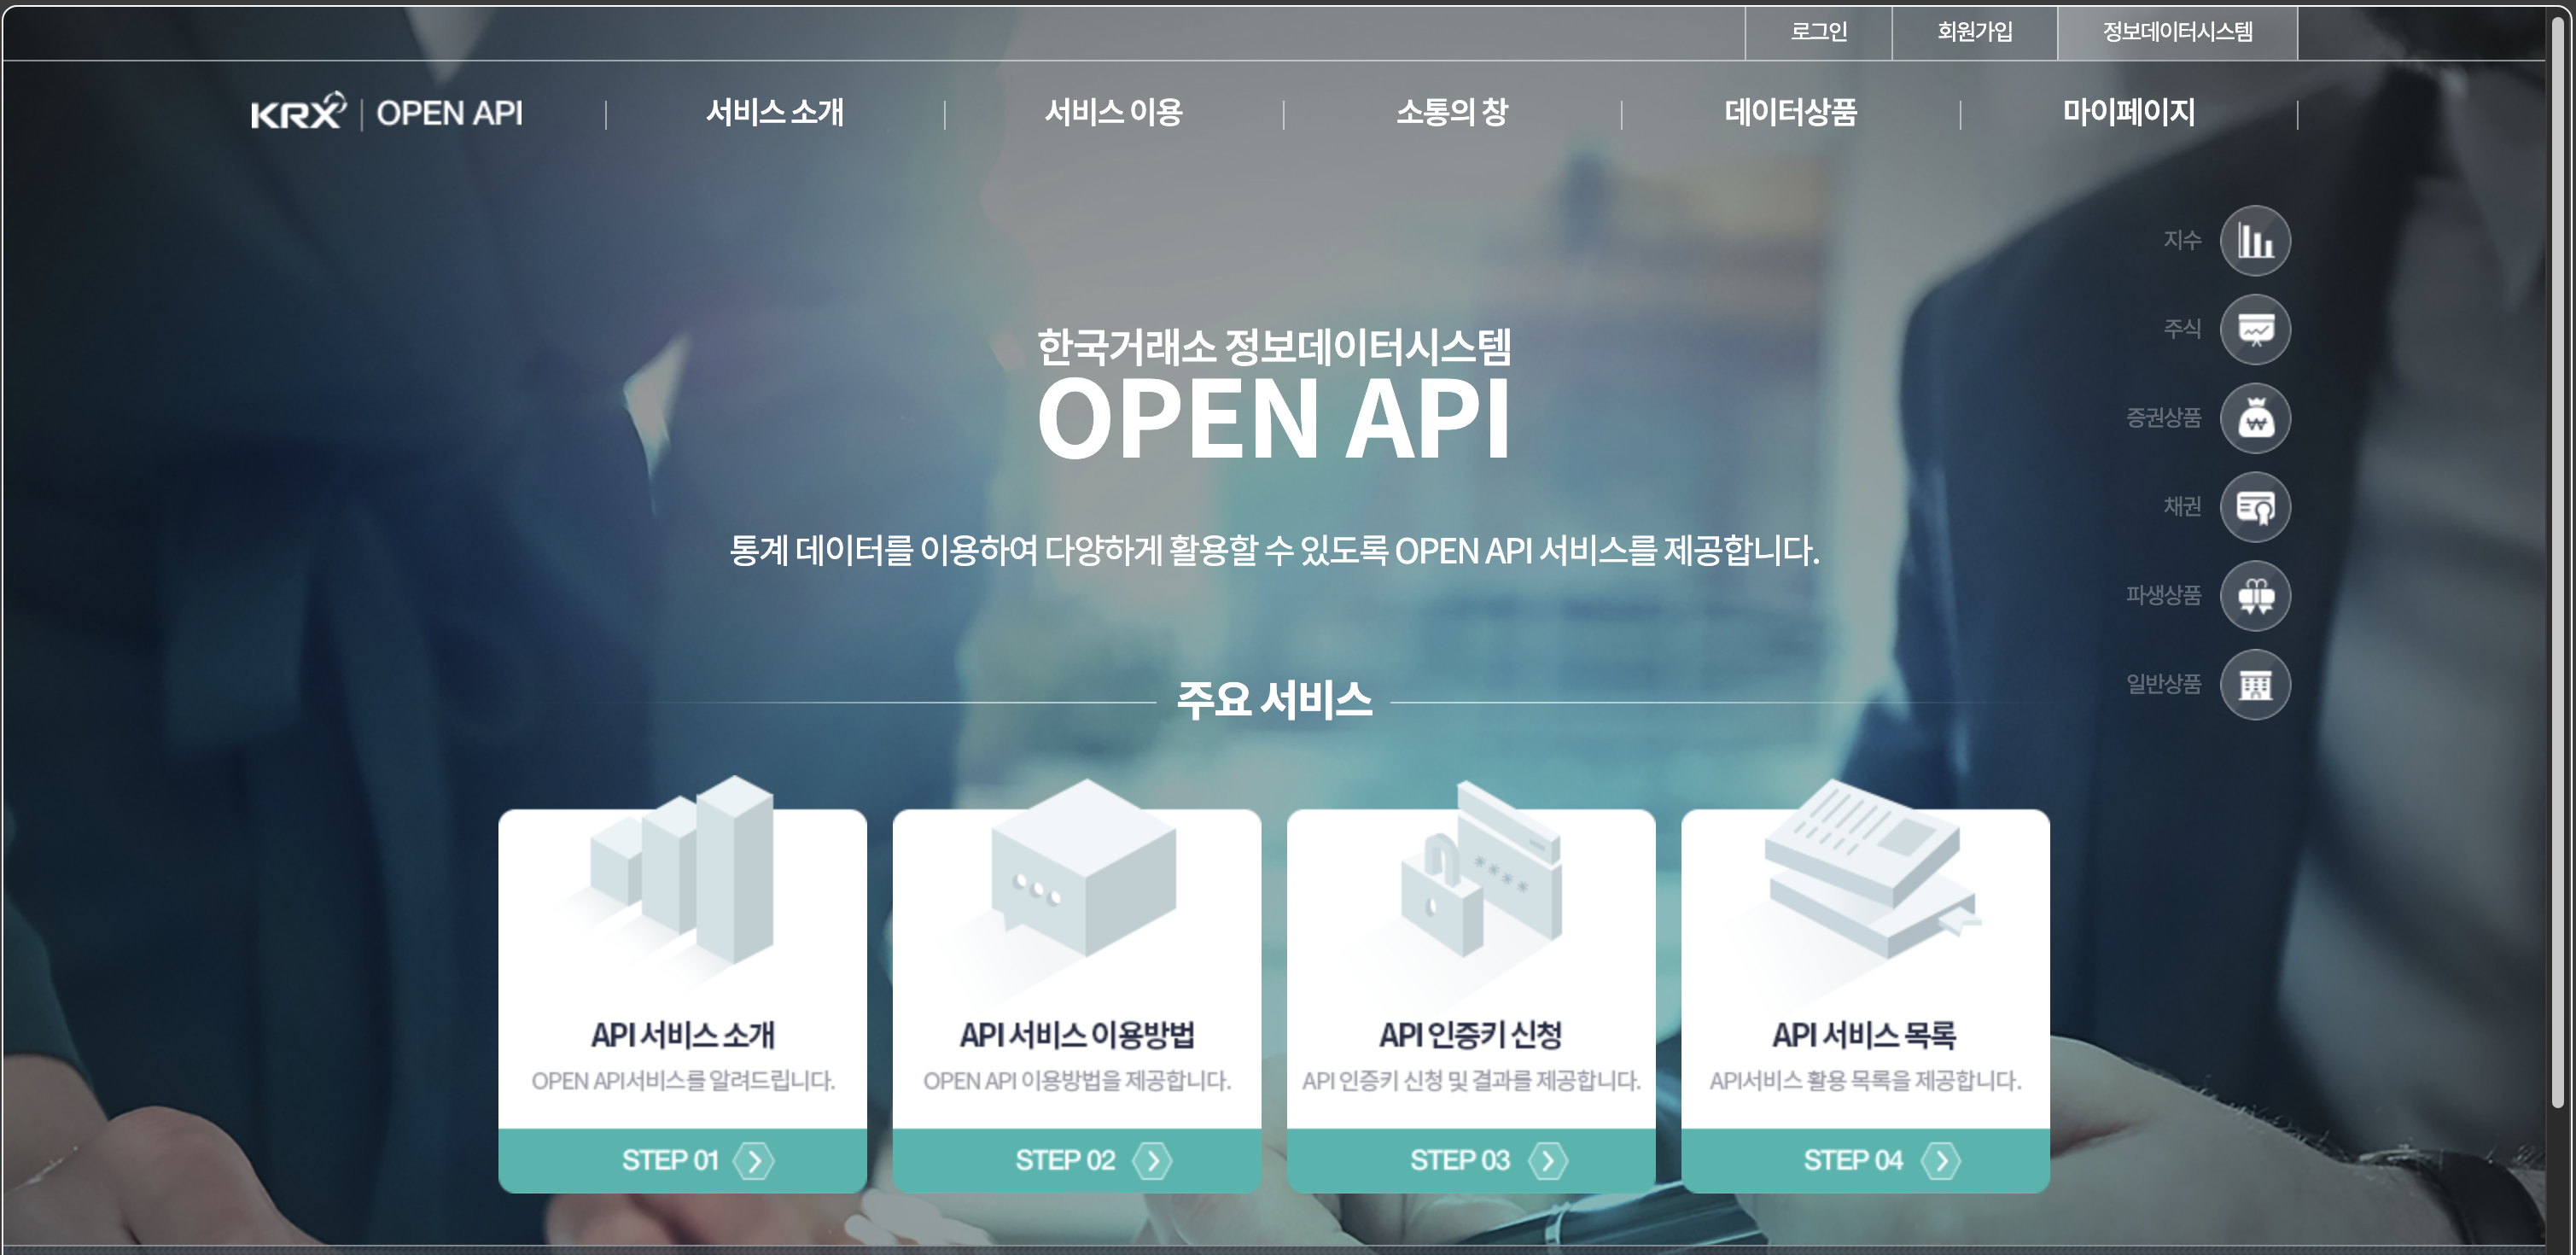
\includegraphics[width=0.6\textwidth,height=\textheight]{image/krxopenapi1.png}
\end{center}

API 호출시 json 데이터를 수집할 수 있으며, 이를 Dataframe(python) 및
tibble(r)로 변환하여 활용하였습니다.

\begin{Shaded}
\begin{Highlighting}[]
\ImportTok{import}\NormalTok{ requests}\OperatorTok{;} \ImportTok{import}\NormalTok{ json}
\NormalTok{url }\OperatorTok{=} \StringTok{\textquotesingle{}http://data{-}dbg.krx.co.kr/svc/sample/apis/drv/opt\_bydd\_trd?basDd=20250312\textquotesingle{}}
\NormalTok{headers }\OperatorTok{=}\NormalTok{ \{}\StringTok{\textquotesingle{}AUTH\_KEY\textquotesingle{}}\NormalTok{: }\StringTok{\textquotesingle{}74D1B99DFBF345BBA3FB4476510A4BED4C78D13A\textquotesingle{}}\NormalTok{\}}
\NormalTok{res }\OperatorTok{=}\NormalTok{ requests.get(url}\OperatorTok{=}\NormalTok{url, headers}\OperatorTok{=}\NormalTok{headers)}\OperatorTok{;}\NormalTok{ res.text}
\end{Highlighting}
\end{Shaded}

\begin{verbatim}
'{"OutBlock_1":[{"BAS_DD":"20250312","PROD_NM":"코스피200 옵션","RGHT_TP_NM":"CALL","ISU_CD":"201W3195","ISU_NM":"코스피200 C 202503 195.0","TDD_CLSPRC":"145.90","CMPPREVDD_PRC":"6.85","TDD_OPNPRC":"144.95","TDD_HGPRC":"146.10","TDD_LWPRC":"144.95","IMP_VOLT":"64.00","NXTDD_BAS_PRC":"145.90","ACC_TRDVOL":"31","ACC_TRDVAL":"1129625000","ACC_OPNINT_QTY":"154"},{"BAS_DD":"20250312","PROD_NM":"코스피200 옵션","RGHT_TP_NM":"CALL","ISU_CD":"201W3197","ISU_NM":"코스피200 C 202503 197.5","TDD_CLSPRC":"-","CMPPREVDD_PRC":"-","TDD_OPNPRC":"-","TDD_HGPRC":"-","TDD_LWPRC":"-","IMP_VOLT":"64.00","NXTDD_BAS_PRC":"143.40","ACC_TRDVOL":"0","ACC_TRDVAL":"0","ACC_OPNINT_QTY":"0"},{"BAS_DD":"20250312","PROD_NM":"코스피200 옵션","RGHT_TP_NM":"CALL","ISU_CD":"201W3200","ISU_NM":"코스피200 C 202503 200.0","TDD_CLSPRC":"140.60","CMPPREVDD_PRC":"5.00","TDD_OPNPRC":"140.00","TDD_HGPRC":"141.15","TDD_LWPRC":"139.95","IMP_VOLT":"64.00","NXTDD_BAS_PRC":"140.60","ACC_TRDVOL":"31","ACC_TRDVAL":"1088750000","ACC_OPNINT_QTY":"290"},{"BAS_DD":"20250312","PROD_NM":"코스피200 옵션","RGHT_TP_NM":"CALL","ISU_CD":"201W3202","ISU_NM":"코스피200 C 202503 202.5","TDD_CLSPRC":"-","CMPPREVDD_PRC":"-","TDD_OPNPRC":"-","TDD_HGPRC":"-","TDD_LWPRC":"-","IMP_VOLT":"64.00","NXTDD_BAS_PRC":"138.40","ACC_TRDVOL":"0","ACC_TRDVAL":"0","ACC_OPNINT_QTY":"0"},{"BAS_DD":"20250312","PROD_NM":"코스피200 옵션","RGHT_TP_NM":"CALL","ISU_CD":"201W3205","ISU_NM":"코스피200 C 202503 205.0","TDD_CLSPRC":"-","CMPPREVDD_PRC":"-","TDD_OPNPRC":"-","TDD_HGPRC":"-","TDD_LWPRC":"-","IMP_VOLT":"64.00","NXTDD_BAS_PRC":"135.90","ACC_TRDVOL":"0","ACC_TRDVAL":"0","ACC_OPNINT_QTY":"0"},{"BAS_DD":"20250312","PROD_NM":"코스피200 옵션","RGHT_TP_NM":"CALL","ISU_CD":"201W3207","ISU_NM":"코스피200 C 202503 207.5","TDD_CLSPRC":"-","CMPPREVDD_PRC":"-","TDD_OPNPRC":"-","TDD_HGPRC":"-","TDD_LWPRC":"-","IMP_VOLT":"64.00","NXTDD_BAS_PRC":"133.40","ACC_TRDVOL":"0","ACC_TRDVAL":"0","ACC_OPNINT_QTY":"0"},{"BAS_DD":"20250312","PROD_NM":"코스피200 옵션","RGHT_TP_NM":"CALL","ISU_CD":"201W3210","ISU_NM":"코스피200 C 202503 210.0","TDD_CLSPRC":"130.60","CMPPREVDD_PRC":"5.60","TDD_OPNPRC":"130.60","TDD_HGPRC":"130.60","TDD_LWPRC":"130.60","IMP_VOLT":"64.00","NXTDD_BAS_PRC":"130.60","ACC_TRDVOL":"1","ACC_TRDVAL":"32650000","ACC_OPNINT_QTY":"20"},{"BAS_DD":"20250312","PROD_NM":"코스피200 옵션","RGHT_TP_NM":"CALL","ISU_CD":"201W3212","ISU_NM":"코스피200 C 202503 212.5","TDD_CLSPRC":"-","CMPPREVDD_PRC":"-","TDD_OPNPRC":"-","TDD_HGPRC":"-","TDD_LWPRC":"-","IMP_VOLT":"62.47","NXTDD_BAS_PRC":"128.40","ACC_TRDVOL":"0","ACC_TRDVAL":"0","ACC_OPNINT_QTY":"0"},{"BAS_DD":"20250312","PROD_NM":"코스피200 옵션","RGHT_TP_NM":"CALL","ISU_CD":"201W3215","ISU_NM":"코스피200 C 202503 215.0","TDD_CLSPRC":"-","CMPPREVDD_PRC":"-","TDD_OPNPRC":"-","TDD_HGPRC":"-","TDD_LWPRC":"-","IMP_VOLT":"60.94","NXTDD_BAS_PRC":"125.90","ACC_TRDVOL":"0","ACC_TRDVAL":"0","ACC_OPNINT_QTY":"59"},{"BAS_DD":"20250312","PROD_NM":"코스피200 옵션","RGHT_TP_NM":"CALL","ISU_CD":"201W3217","ISU_NM":"코스피200 C 202503 217.5","TDD_CLSPRC":"-","CMPPREVDD_PRC":"-","TDD_OPNPRC":"-","TDD_HGPRC":"-","TDD_LWPRC":"-","IMP_VOLT":"59.42","NXTDD_BAS_PRC":"123.40","ACC_TRDVOL":"0","ACC_TRDVAL":"0","ACC_OPNINT_QTY":"0"}]}'
\end{verbatim}

\end{tcolorbox}

수집한 데이터는 \textbf{R을 이용하여 전처리}하였으며, 두개의
데이터셋으로 요약하였습니다.

\begin{enumerate}
\def\labelenumi{\arabic{enumi}.}
\tightlist
\item
  \textbf{포트폴리오 기본 정보} : 옵션 만기일(매주), 옵션 보유일,
  MMF금리, Kospi200, 전일 V-K200, 거래대상옵션 정보
\end{enumerate}

\begin{longtable}[]{@{}
  >{\raggedleft\arraybackslash}p{(\columnwidth - 16\tabcolsep) * \real{0.1098}}
  >{\raggedleft\arraybackslash}p{(\columnwidth - 16\tabcolsep) * \real{0.1220}}
  >{\raggedleft\arraybackslash}p{(\columnwidth - 16\tabcolsep) * \real{0.1098}}
  >{\raggedleft\arraybackslash}p{(\columnwidth - 16\tabcolsep) * \real{0.0854}}
  >{\raggedleft\arraybackslash}p{(\columnwidth - 16\tabcolsep) * \real{0.1098}}
  >{\raggedleft\arraybackslash}p{(\columnwidth - 16\tabcolsep) * \real{0.1220}}
  >{\raggedleft\arraybackslash}p{(\columnwidth - 16\tabcolsep) * \real{0.0732}}
  >{\raggedleft\arraybackslash}p{(\columnwidth - 16\tabcolsep) * \real{0.1341}}
  >{\raggedleft\arraybackslash}p{(\columnwidth - 16\tabcolsep) * \real{0.1341}}@{}}
\toprule\noalign{}
\begin{minipage}[b]{\linewidth}\raggedleft
BAS\_DD
\end{minipage} & \begin{minipage}[b]{\linewidth}\raggedleft
VOL
\end{minipage} & \begin{minipage}[b]{\linewidth}\raggedleft
DIFF\_DAY
\end{minipage} & \begin{minipage}[b]{\linewidth}\raggedleft
MMF
\end{minipage} & \begin{minipage}[b]{\linewidth}\raggedleft
KOSPI200
\end{minipage} & \begin{minipage}[b]{\linewidth}\raggedleft
LAG\_VK200
\end{minipage} & \begin{minipage}[b]{\linewidth}\raggedleft
PRIOR
\end{minipage} & \begin{minipage}[b]{\linewidth}\raggedleft
TARGET\_C\_K
\end{minipage} & \begin{minipage}[b]{\linewidth}\raggedleft
TARGET\_P\_K
\end{minipage} \\
\midrule\noalign{}
\endhead
\bottomrule\noalign{}
\endlastfoot
20241219 & 0.0248719 & 7 & 0.0334 & 322.38 & 17.96 & 24124 & 332.5 &
312.5 \\
20241212 & 0.0285279 & 7 & 0.0335 & 329.04 & 20.60 & 24123 & 340.0 &
317.5 \\
20241205 & 0.0295527 & 7 & 0.0341 & 323.87 & 21.34 & 24122 & 335.0 &
312.5 \\
20241128 & 0.0252043 & 7 & 0.0340 & 331.45 & 18.20 & 24121 & 340.0 &
322.5 \\
20241121 & 0.0276001 & 7 & 0.0344 & 329.49 & 19.93 & 24114 & 340.0 &
320.0 \\
20241114 & 0.0344274 & 7 & 0.0340 & 317.70 & 24.86 & 24113 & 330.0 &
305.0 \\
\end{longtable}

\begin{enumerate}
\def\labelenumi{\arabic{enumi}.}
\setcounter{enumi}{1}
\tightlist
\item
  \textbf{거래대상옵션 정보} : 포트폴리오 기본 정보에 대응되는
  거래대상옵션의 종가, 거래량(0인 경우 제외)
\end{enumerate}

\begin{longtable}[]{@{}
  >{\raggedleft\arraybackslash}p{(\columnwidth - 8\tabcolsep) * \real{0.1034}}
  >{\raggedleft\arraybackslash}p{(\columnwidth - 8\tabcolsep) * \real{0.1954}}
  >{\raggedleft\arraybackslash}p{(\columnwidth - 8\tabcolsep) * \real{0.1954}}
  >{\raggedleft\arraybackslash}p{(\columnwidth - 8\tabcolsep) * \real{0.2529}}
  >{\raggedleft\arraybackslash}p{(\columnwidth - 8\tabcolsep) * \real{0.2529}}@{}}
\toprule\noalign{}
\begin{minipage}[b]{\linewidth}\raggedleft
BAS\_DD
\end{minipage} & \begin{minipage}[b]{\linewidth}\raggedleft
PRICE\_TARGET\_C\_K
\end{minipage} & \begin{minipage}[b]{\linewidth}\raggedleft
PRICE\_TARGET\_P\_K
\end{minipage} & \begin{minipage}[b]{\linewidth}\raggedleft
ACC\_TRDVOL\_TARGET\_C\_K
\end{minipage} & \begin{minipage}[b]{\linewidth}\raggedleft
ACC\_TRDVOL\_TARGET\_P\_K
\end{minipage} \\
\midrule\noalign{}
\endhead
\bottomrule\noalign{}
\endlastfoot
20241219 & 0.29 & 0.74 & 343 & 137 \\
20241212 & 0.42 & 0.78 & 190 & 196 \\
20241205 & 0.44 & 0.91 & 65452 & 51417 \\
20241128 & 0.34 & 0.43 & 288 & 201 \\
20241121 & 0.37 & 0.53 & 115 & 201 \\
20241114 & 0.43 & 0.74 & 329 & 165 \\
\end{longtable}

이를 통해 매도수량, 프리미엄, 이자수익, 권리행사손실 등을 산출하여
\textbf{포트폴리오를 구현}하였습니다.

\begin{longtable}[]{@{}
  >{\raggedleft\arraybackslash}p{(\columnwidth - 14\tabcolsep) * \real{0.1154}}
  >{\raggedleft\arraybackslash}p{(\columnwidth - 14\tabcolsep) * \real{0.1282}}
  >{\raggedleft\arraybackslash}p{(\columnwidth - 14\tabcolsep) * \real{0.1154}}
  >{\raggedleft\arraybackslash}p{(\columnwidth - 14\tabcolsep) * \real{0.1154}}
  >{\raggedleft\arraybackslash}p{(\columnwidth - 14\tabcolsep) * \real{0.1154}}
  >{\raggedleft\arraybackslash}p{(\columnwidth - 14\tabcolsep) * \real{0.1282}}
  >{\raggedleft\arraybackslash}p{(\columnwidth - 14\tabcolsep) * \real{0.1410}}
  >{\raggedleft\arraybackslash}p{(\columnwidth - 14\tabcolsep) * \real{0.1410}}@{}}
\toprule\noalign{}
\begin{minipage}[b]{\linewidth}\raggedleft
BAS\_DD
\end{minipage} & \begin{minipage}[b]{\linewidth}\raggedleft
VOL
\end{minipage} & \begin{minipage}[b]{\linewidth}\raggedleft
SELL\_AMT
\end{minipage} & \begin{minipage}[b]{\linewidth}\raggedleft
PREMIUM
\end{minipage} & \begin{minipage}[b]{\linewidth}\raggedleft
INTEREST
\end{minipage} & \begin{minipage}[b]{\linewidth}\raggedleft
EXERCISE
\end{minipage} & \begin{minipage}[b]{\linewidth}\raggedleft
REVENUE
\end{minipage} & \begin{minipage}[b]{\linewidth}\raggedleft
RATE
\end{minipage} \\
\midrule\noalign{}
\endhead
\bottomrule\noalign{}
\endlastfoot
20200102 & 0.0203434 & 137.7648 & 29963837 & 2789154 & 0 & 32752991 &
0.0032753 \\
20200109 & 0.0221160 & 135.8650 & 20040080 & 2844044 & 9510547 &
13373578 & 0.0013374 \\
20200116 & 0.0185154 & 132.1091 & 18825550 & 2824485 & 0 & 21650035 &
0.0021650 \\
20200123 & 0.0197895 & 132.3058 & 23815037 & 2787444 & 219296795 &
-192694314 & -0.0192694 \\
20200130 & 0.0235286 & 138.7107 & 45080972 & 2793358 & 109234664 &
-61360333 & -0.0061360 \\
20200206 & 0.0252458 & 133.0451 & 46565774 & 2774504 & 0 & 49340278 &
0.0049340 \\
\end{longtable}

\newpage

\begin{tcolorbox}[enhanced jigsaw, bottomtitle=1mm, breakable, coltitle=black, opacityback=0, titlerule=0mm, left=2mm, colbacktitle=quarto-callout-important-color!10!white, toptitle=1mm, colframe=quarto-callout-important-color-frame, bottomrule=.15mm, opacitybacktitle=0.6, leftrule=.75mm, title=\textcolor{quarto-callout-important-color}{\faExclamation}\hspace{0.5em}{변동성 조정 방법에 따른 행사가격 범위 추이(과거 5년)}, arc=.35mm, toprule=.15mm, rightrule=.15mm, colback=white]

V-Kospi200과 연동한 행사가격의 범위는 지난 5년간 \textbf{1.6\%
\textasciitilde{} 8.7\%까지 광범위하게 형성}되었습니다.

코스피200이 급등락하는 경우 범위가 넓게 형성되고 보합장에서는 좁게
형성되는 추이를 확인할 수 있으며, 이를 월환산(\(\times\sqrt{4}\))하여
기존 5\%와 비교하면 \textbf{지수의 상황에 따라 유동적으로 조절되고
있음}을 의미합니다.

\hfill\break

\textbf{\emph{그래프2 : 월평균 코스피200지수(적색) 및 행사가격
범위(청색)}}

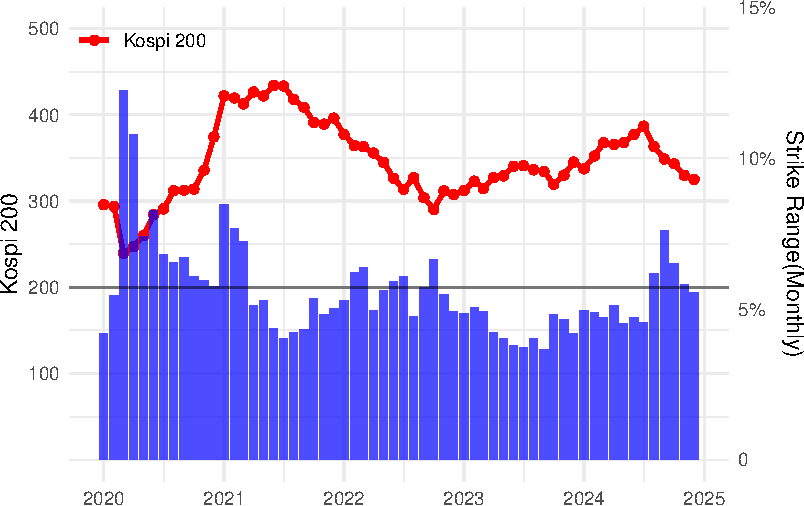
\includegraphics{사례_과제_files/figure-pdf/unnamed-chunk-6-1.pdf}

\end{tcolorbox}

\newpage

\subsection*{Backtesting 성과}\label{backtesting-uxc131uxacfc}
\addcontentsline{toc}{subsection}{Backtesting 성과}

\textbf{지난 5년간(2020\textasciitilde2024) VW양매도와 코스피200지수 /
OTM 5\% 양매도를 비교}해보았습니다.

\textbf{\emph{표1 : 연도별 변동성 조정 위클리 양매도 포트폴리오 및
코스피200지수 성과}}

\begin{longtable}[]{@{}
  >{\raggedright\arraybackslash}p{(\columnwidth - 16\tabcolsep) * \real{0.0694}}
  >{\raggedleft\arraybackslash}p{(\columnwidth - 16\tabcolsep) * \real{0.0972}}
  >{\raggedleft\arraybackslash}p{(\columnwidth - 16\tabcolsep) * \real{0.1528}}
  >{\raggedleft\arraybackslash}p{(\columnwidth - 16\tabcolsep) * \real{0.1111}}
  >{\raggedleft\arraybackslash}p{(\columnwidth - 16\tabcolsep) * \real{0.1250}}
  >{\raggedleft\arraybackslash}p{(\columnwidth - 16\tabcolsep) * \real{0.0694}}
  >{\raggedleft\arraybackslash}p{(\columnwidth - 16\tabcolsep) * \real{0.1111}}
  >{\raggedleft\arraybackslash}p{(\columnwidth - 16\tabcolsep) * \real{0.0972}}
  >{\raggedleft\arraybackslash}p{(\columnwidth - 16\tabcolsep) * \real{0.1667}}@{}}
\toprule\noalign{}
\begin{minipage}[b]{\linewidth}\raggedright
YEAR
\end{minipage} & \begin{minipage}[b]{\linewidth}\raggedleft
Expiry
\end{minipage} & \begin{minipage}[b]{\linewidth}\raggedleft
NoExercise
\end{minipage} & \begin{minipage}[b]{\linewidth}\raggedleft
Premium
\end{minipage} & \begin{minipage}[b]{\linewidth}\raggedleft
Interest
\end{minipage} & \begin{minipage}[b]{\linewidth}\raggedleft
Loss
\end{minipage} & \begin{minipage}[b]{\linewidth}\raggedleft
Revenue
\end{minipage} & \begin{minipage}[b]{\linewidth}\raggedleft
Return
\end{minipage} & \begin{minipage}[b]{\linewidth}\raggedleft
Return\_K200
\end{minipage} \\
\midrule\noalign{}
\endhead
\bottomrule\noalign{}
\endlastfoot
2020 & 50 & 0.74 & 4385 & 184 & 5338 & -769 & -0.04 & 0.33 \\
2021 & 47 & 0.91 & 2974 & 142 & 728 & 2387 & 0.12 & 0.01 \\
2022 & 52 & 0.79 & 3304 & 421 & 4152 & -427 & -0.03 & -0.26 \\
2023 & 52 & 0.81 & 2456 & 732 & 1758 & 1430 & 0.08 & 0.23 \\
2024 & 49 & 0.80 & 3697 & 719 & 3454 & 962 & 0.05 & -0.11 \\
\end{longtable}

\textbf{\emph{표2 : 연도별 일반 양매도 포트폴리오 및 코스피200지수
성과}}

\begin{longtable}[]{@{}
  >{\raggedright\arraybackslash}p{(\columnwidth - 16\tabcolsep) * \real{0.0685}}
  >{\raggedleft\arraybackslash}p{(\columnwidth - 16\tabcolsep) * \real{0.0959}}
  >{\raggedleft\arraybackslash}p{(\columnwidth - 16\tabcolsep) * \real{0.1507}}
  >{\raggedleft\arraybackslash}p{(\columnwidth - 16\tabcolsep) * \real{0.1096}}
  >{\raggedleft\arraybackslash}p{(\columnwidth - 16\tabcolsep) * \real{0.1233}}
  >{\raggedleft\arraybackslash}p{(\columnwidth - 16\tabcolsep) * \real{0.0822}}
  >{\raggedleft\arraybackslash}p{(\columnwidth - 16\tabcolsep) * \real{0.1096}}
  >{\raggedleft\arraybackslash}p{(\columnwidth - 16\tabcolsep) * \real{0.0959}}
  >{\raggedleft\arraybackslash}p{(\columnwidth - 16\tabcolsep) * \real{0.1644}}@{}}
\toprule\noalign{}
\begin{minipage}[b]{\linewidth}\raggedright
YEAR
\end{minipage} & \begin{minipage}[b]{\linewidth}\raggedleft
Expiry
\end{minipage} & \begin{minipage}[b]{\linewidth}\raggedleft
NoExercise
\end{minipage} & \begin{minipage}[b]{\linewidth}\raggedleft
Premium
\end{minipage} & \begin{minipage}[b]{\linewidth}\raggedleft
Interest
\end{minipage} & \begin{minipage}[b]{\linewidth}\raggedleft
Loss
\end{minipage} & \begin{minipage}[b]{\linewidth}\raggedleft
Revenue
\end{minipage} & \begin{minipage}[b]{\linewidth}\raggedleft
Return
\end{minipage} & \begin{minipage}[b]{\linewidth}\raggedleft
Return\_K200
\end{minipage} \\
\midrule\noalign{}
\endhead
\bottomrule\noalign{}
\endlastfoot
2020 & 12 & 0.58 & 16507 & 847 & 37851 & -20497 & -0.23 & 0.33 \\
2021 & 12 & 1.00 & 9887 & 605 & 0 & 10492 & 0.13 & 0.01 \\
2022 & 12 & 0.50 & 10207 & 1819 & 15098 & -3071 & -0.04 & -0.26 \\
2023 & 12 & 0.83 & 4591 & 3176 & 884 & 6883 & 0.09 & 0.23 \\
2024 & 12 & 0.75 & 9850 & 3072 & 9589 & 3333 & 0.04 & -0.11 \\
\end{longtable}

\begin{tcolorbox}[enhanced jigsaw, breakable, colframe=quarto-callout-color-frame, bottomrule=.15mm, arc=.35mm, opacityback=0, leftrule=.75mm, left=2mm, toprule=.15mm, rightrule=.15mm, colback=white]

\textbf{YEAR} : 산출대상 연도 / \textbf{Expiry} : 옵션만기 횟수
(프리미엄 수익 발생 횟수)

\textbf{NoExercise} : 옵션만기일에 행사되지 않은 비율 (손실이 발생하지
않은 거래일 비율)

\textbf{Premium} : 평균 옵션 프리미엄 수익 (만원) / \textbf{Interest} :
원금 및 프리미엄에서 발생한 평균 이자수익 (만원)

\textbf{Loss} : 옵션권리행사로 인한 평균 손실 (미행사 포함) /
\textbf{Revenue} : 평균 이익 (Premium + Interest - Loss)

\textbf{Return} : 포트폴리오의 연환산 수익률 / \textbf{Return\_K200} :
코스피200지수의 연환산 수익률

\end{tcolorbox}

\textbf{변동성 조정 위클리 양매도 포트폴리오}의 주요 성과는 다음과
같습니다.

\begin{enumerate}
\def\labelenumi{\arabic{enumi}.}
\tightlist
\item
  옵션 매도주기 축소(월간 \(\rightarrow\) 주간) : \textbf{현금흐름 개선
  및 프리미엄 수익 극대화}
\end{enumerate}

\begin{itemize}
\tightlist
\item
  VW양매도 포트폴리오는 연평균 50회의 수익이 발생하는 반면, 일반 양매도
  포트폴리오는 12회(월1회) 발생.
\item
  1회 발생 수익은 4배 미만으로 감소하여 평균 수익이 증가하였고,
  수익주기가 짧아지면서 현금유동성 개선
\end{itemize}

\begin{enumerate}
\def\labelenumi{\arabic{enumi}.}
\setcounter{enumi}{1}
\tightlist
\item
  행사가격 범위 조정(5\% \(\rightarrow\) \(\sigma\)연동) :
  \textbf{포트폴리오 안정성 증가 및 리스크 축소}
\end{enumerate}

\begin{itemize}
\tightlist
\item
  일반 양매도 전략의 손실발생비율(권리행사비율)은 시장 상황에 따라
  0\textasciitilde50\%까지 큰 폭으로 변동
\item
  반면, 본 포트폴리오는 행사가격 범위를 변동성 수준에 조정하므로 비율이
  10\textasciitilde30\%수준으로 안정화
\item
  손실에 대한 예측가능성 및 포트폴리오 변동성이 개선되었으며 1회 손실도
  감내 가능한 수준으로 축소
\end{itemize}

\begin{enumerate}
\def\labelenumi{\arabic{enumi}.}
\setcounter{enumi}{2}
\tightlist
\item
  \textbf{소결 : VW양매도 전략은 수익률, 리스크 측면에서 코스피200지수
  및 일반 양매도 전략을 Outperform}
\end{enumerate}

\newpage

\textbf{\emph{그래프3, 4 : 지난 5년 및 3년간 코스피200지수, VW양매도,
5\%양매도 누적수익률 및 초과수익}}

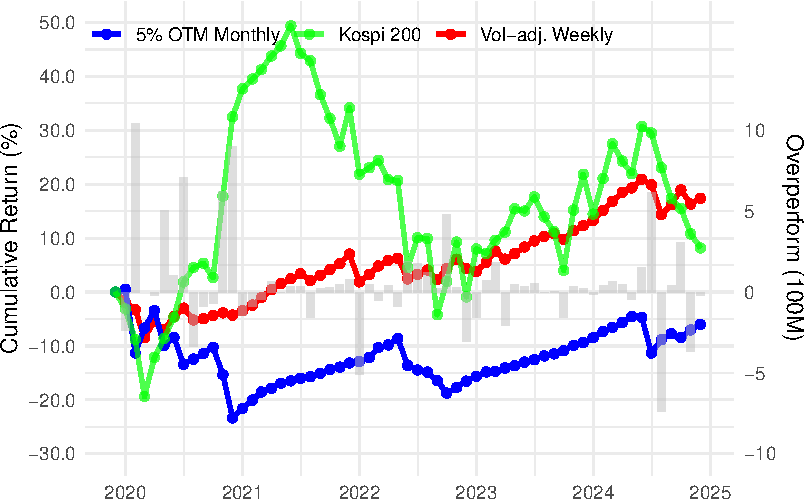
\includegraphics{사례_과제_files/figure-pdf/unnamed-chunk-9-1.pdf}

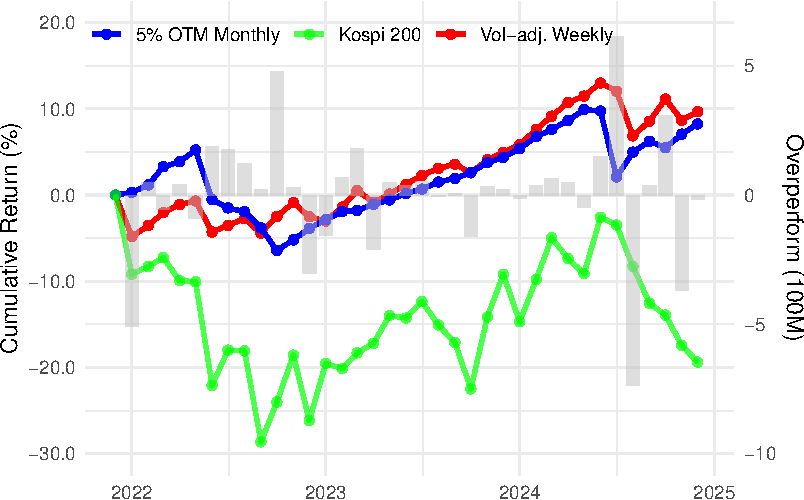
\includegraphics{사례_과제_files/figure-pdf/unnamed-chunk-10-1.pdf}

\textbf{\emph{표3 : 연도별 VW양매도, 일반 양매도, 코스피200지수의 수익률
및 변동성(월간수익률의 연환산)}}

\begin{longtable}[]{@{}
  >{\raggedright\arraybackslash}p{(\columnwidth - 12\tabcolsep) * \real{0.0758}}
  >{\raggedleft\arraybackslash}p{(\columnwidth - 12\tabcolsep) * \real{0.1818}}
  >{\raggedleft\arraybackslash}p{(\columnwidth - 12\tabcolsep) * \real{0.1667}}
  >{\raggedleft\arraybackslash}p{(\columnwidth - 12\tabcolsep) * \real{0.1818}}
  >{\raggedleft\arraybackslash}p{(\columnwidth - 12\tabcolsep) * \real{0.1364}}
  >{\raggedleft\arraybackslash}p{(\columnwidth - 12\tabcolsep) * \real{0.1212}}
  >{\raggedleft\arraybackslash}p{(\columnwidth - 12\tabcolsep) * \real{0.1364}}@{}}
\toprule\noalign{}
\begin{minipage}[b]{\linewidth}\raggedright
YEAR
\end{minipage} & \begin{minipage}[b]{\linewidth}\raggedleft
Return\_main
\end{minipage} & \begin{minipage}[b]{\linewidth}\raggedleft
Return\_sub
\end{minipage} & \begin{minipage}[b]{\linewidth}\raggedleft
Return\_K200
\end{minipage} & \begin{minipage}[b]{\linewidth}\raggedleft
Vol\_main
\end{minipage} & \begin{minipage}[b]{\linewidth}\raggedleft
Vol\_sub
\end{minipage} & \begin{minipage}[b]{\linewidth}\raggedleft
Vol\_K200
\end{minipage} \\
\midrule\noalign{}
\endhead
\bottomrule\noalign{}
\endlastfoot
2020 & -0.04 & -0.23 & 0.33 & 0.08 & 0.19 & 0.27 \\
2021 & 0.12 & 0.13 & 0.01 & 0.03 & 0.02 & 0.11 \\
2022 & -0.03 & -0.04 & -0.26 & 0.08 & 0.08 & 0.25 \\
2023 & 0.08 & 0.09 & 0.23 & 0.04 & 0.01 & 0.17 \\
2024 & 0.05 & 0.04 & -0.11 & 0.07 & 0.08 & 0.16 \\
\end{longtable}

그래프와 표를 통해 \textbf{VW양매도 전략}이 타 전략 대비
\textbf{안정적이고 높은 수익을 실현}하였음을 확인할 수 있었습니다.

\subsection*{한계점}\label{uxd55cuxacc4uxc810}
\addcontentsline{toc}{subsection}{한계점}

그러나, \textbf{행사가격 범위가 전일 V-Kospi200 지수에 따라 결정}되므로
옵션 매도일 및 보유기간 중 V-Kospi200 지수가 급등락하는 경우
\textbf{시장 변동성을 적절히 반영되지 않을 가능성}이 있습니다.

\begin{itemize}
\tightlist
\item
  당일 장중 지수를 사용할 수 있겠으나 종가보다 신뢰성이 높다고 보기
  어렵고, 당일 종가는 매도시점에서 확인 불가
\item
  보유기간 중 V-Kospi200의 변동에 따라 옵션 행사가격을 리밸런싱하면 보다
  정확히 변동성을 반영할 수 있으나, 잦은 거래로 인해 수반되는 비용이
  급증
\item
  시장 변동성이 적절히 반영되지 않는 경우, 프리미엄 수익성이 낮아지고
  옵션 권리행사 위험이 증가할 수 있음
\end{itemize}

또한, \textbf{실제로 VW양매도 포트폴리오를 운영}한다면 \textbf{거래비용
및 유동성 등의 한계점}으로 인해 보완해야할 점이 있으며 이 과정에서
초과수익률 등의 \textbf{성과가 다소 희석}될 것으로 예상됩니다.

\begin{itemize}
\tightlist
\item
  수수료/유동성 등으로 인해 자주 옵션을 매도하는 전략 특성상 거래비용
  상승이 수반됨
\item
  월물 옵션 대비 위클리옵션의 유동성이 낮아, 변동성 확대 국면에서 원하는
  위클리옵션의 거래가 없을 수 있음
\end{itemize}

\section*{4. 포트폴리오 검증 ('25.3.13 \textasciitilde{}
4.10)}\label{uxd3ecuxd2b8uxd3f4uxb9acuxc624-uxac80uxc99d-25.3.13-4.10}
\addcontentsline{toc}{section}{4. 포트폴리오 검증 ('25.3.13
\textasciitilde{} 4.10)}

\markright{4. 포트폴리오 검증 ('25.3.13 \textasciitilde{} 4.10)}

포트폴리오의 성과 검증을 위해 \textbf{'25년 3월 옵션만기일부터 1개월간의
성과를 측정}해보겠습니다.

\textbf{Backtesting과 동일한 방식으로 진행}하였으며, 날짜 등 일부를
제외하고 동일 코드를 재사용하였습니다.

\textbf{\emph{표4 : 검증기간('25.3.13 \textasciitilde{} 4.10) VW양매도
및 일반 양매도 전략 성과}}

\begin{longtable}[]{@{}
  >{\raggedleft\arraybackslash}p{(\columnwidth - 12\tabcolsep) * \real{0.1343}}
  >{\raggedright\arraybackslash}p{(\columnwidth - 12\tabcolsep) * \real{0.2985}}
  >{\raggedleft\arraybackslash}p{(\columnwidth - 12\tabcolsep) * \real{0.1194}}
  >{\raggedleft\arraybackslash}p{(\columnwidth - 12\tabcolsep) * \real{0.1343}}
  >{\raggedleft\arraybackslash}p{(\columnwidth - 12\tabcolsep) * \real{0.0896}}
  >{\raggedleft\arraybackslash}p{(\columnwidth - 12\tabcolsep) * \real{0.1194}}
  >{\raggedleft\arraybackslash}p{(\columnwidth - 12\tabcolsep) * \real{0.1045}}@{}}
\toprule\noalign{}
\begin{minipage}[b]{\linewidth}\raggedleft
BAS\_DD
\end{minipage} & \begin{minipage}[b]{\linewidth}\raggedright
Group
\end{minipage} & \begin{minipage}[b]{\linewidth}\raggedleft
Premium
\end{minipage} & \begin{minipage}[b]{\linewidth}\raggedleft
Interest
\end{minipage} & \begin{minipage}[b]{\linewidth}\raggedleft
Loss
\end{minipage} & \begin{minipage}[b]{\linewidth}\raggedleft
Revenue
\end{minipage} & \begin{minipage}[b]{\linewidth}\raggedleft
Return
\end{minipage} \\
\midrule\noalign{}
\endhead
\bottomrule\noalign{}
\endlastfoot
20250313 & Monthly & 12653 & 2400 & 0 & 15053 & 0.02 \\
20250313 & Vol-adj. Weekly & 5624 & 596 & 2929 & 3291 & 0.00 \\
20250320 & Vol-adj. Weekly & 2687 & 587 & 0 & 3274 & 0.00 \\
20250327 & Vol-adj. Weekly & 4283 & 578 & 20214 & -15353 & -0.02 \\
20250403 & Vol-adj. Weekly & 11594 & 578 & 0 & 12173 & 0.01 \\
81001363 & Vol-adj. Weekly Sum & 24188 & 2338 & 23142 & 3384 & 0.00 \\
\end{longtable}

\textbf{검증기간 중 VW양매도 전략은 옵션을 4회 매도하였고, 일반 양매도는
1회 매도}하였습니다.

VW양매도 전략의 \textbf{프리미엄이 4회 발생하면서 수익성은
개선}되었지만, 세번째 매도시기에 \textbf{큰 손실이 발생하면서 순이익이
악화}되었습니다. 벡테스팅 결과와 비교할 때 \textbf{상반된 결과}입니다.

그 \textbf{원인은 최근 트럼프 행정부의 관세 부과 정책의 영향}으로,
증시가 이례적으로 급등락한 데에서 찾을 수 있었습니다.

\newpage

\textbf{\emph{그래프5 : 검증기간('25.3.13 \textasciitilde{} 4.10)
Kospi200 및 V-Kospi200 지수 추이}}

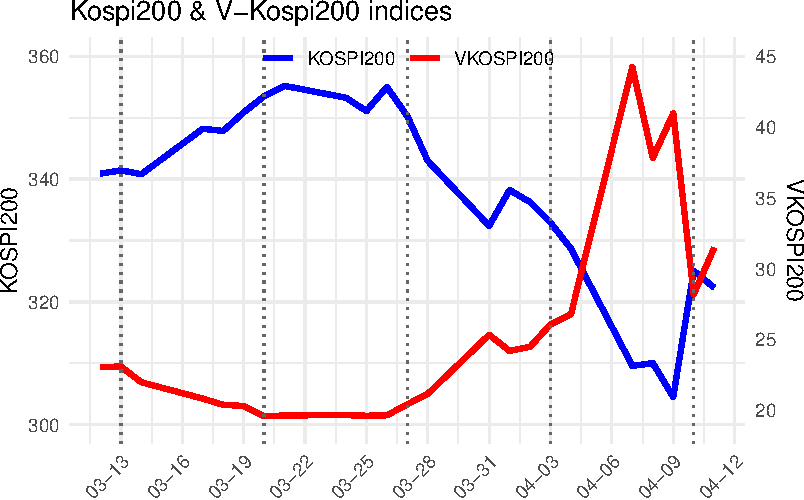
\includegraphics{사례_과제_files/figure-pdf/unnamed-chunk-14-1.pdf}

먼저, \textbf{3.27일 예상변동성(V-K200)이 낮아 행사가격 범위가 좁게
형성}되어 VW양매도 전략이 실행되었고, 이후 관세 정책 영향으로 지수가
급락하면서 \textbf{큰 손실이 발생}하게 되었습니다.

반면 \textbf{월별 전략은 만기 직전에 관세가 연기}되면서 \textbf{증시가
회복}하였고(304 \textgreater{} 325), 손실을 피하게 되었습니다.

다소 아쉬운 결과이나, \textbf{VW양매도 전략의 한계점과 특수한 상황에서는
오히려 불리하다는 점}을 알 수 있었습니다.

\begin{enumerate}
\def\labelenumi{\arabic{enumi}.}
\tightlist
\item
  VW양매도 전략은 \textbf{시장 변동성이 적절히 반영되지 않을 가능성}이
  있고, 이 경우 예기치 못한 손실이 발생할 수 있음
\item
  \textbf{옵션 만기가 짧은 것은 일반적}으로 수익성, 유동성 등에서
  \textbf{장점}이 있으나, \textbf{증시가 급락 후 회복하는 상황에서는
  만기가 긴 옵션이 유리}할 수 있음
\end{enumerate}

\newpage

\section*{5. Appendix : Python, R code}\label{appendix-python-r-code}
\addcontentsline{toc}{section}{5. Appendix : Python, R code}

\markright{5. Appendix : Python, R code}

\subsection*{Pyhon code : 데이터 수집 및
전처리}\label{pyhon-code-uxb370uxc774uxd130-uxc218uxc9d1-uxbc0f-uxc804uxcc98uxb9ac}
\addcontentsline{toc}{subsection}{Pyhon code : 데이터 수집 및 전처리}

\begin{Shaded}
\begin{Highlighting}[]
\ImportTok{import}\NormalTok{ requests}
\ImportTok{import}\NormalTok{ json}
\ImportTok{import}\NormalTok{ pandas }\ImportTok{as}\NormalTok{ pd}
\ImportTok{import}\NormalTok{ aiohttp}
\ImportTok{import}\NormalTok{ asyncio}

\CommentTok{\# KRX OpenAPI 예시}
\NormalTok{url }\OperatorTok{=} \StringTok{\textquotesingle{}http://data{-}dbg.krx.co.kr/svc/sample/apis/drv/opt\_bydd\_trd?basDd=20250312\textquotesingle{}}
\NormalTok{headers }\OperatorTok{=}\NormalTok{ \{}\StringTok{\textquotesingle{}AUTH\_KEY\textquotesingle{}}\NormalTok{: }\StringTok{\textquotesingle{}74D1B99DFBF345BBA3FB4476510A4BED4C78D13A\textquotesingle{}}\NormalTok{\}}
\NormalTok{res }\OperatorTok{=}\NormalTok{ requests.get(url}\OperatorTok{=}\NormalTok{url, headers}\OperatorTok{=}\NormalTok{headers)}
\NormalTok{res.text}

\CommentTok{\# KRX OpenAPI를 이용한 옵션 데이터 수집 (네트워크 병렬 처리)}
\NormalTok{idx\_data }\OperatorTok{=}\NormalTok{ pd.read\_csv(}\StringTok{\textquotesingle{}data/idx\_data.csv\textquotesingle{}}\NormalTok{)}
\NormalTok{url }\OperatorTok{=} \StringTok{\textquotesingle{}http://data{-}dbg.krx.co.kr/svc/apis/drv/opt\_bydd\_trd?basDd=\textquotesingle{}}
\NormalTok{key }\OperatorTok{=} \StringTok{\textquotesingle{}BDFA640BBCE84C4B8A465EA024D50D6F3FD909FF\textquotesingle{}}

\ControlFlowTok{async} \KeywordTok{def}\NormalTok{ fetch(session, url, bas\_dd):}
    \ControlFlowTok{async} \ControlFlowTok{with}\NormalTok{ session.get(url }\OperatorTok{+}\NormalTok{ bas\_dd, headers}\OperatorTok{=}\NormalTok{\{}\StringTok{\textquotesingle{}AUTH\_KEY\textquotesingle{}}\NormalTok{: key\}) }\ImportTok{as}\NormalTok{ response:}
        \ControlFlowTok{return} \ControlFlowTok{await}\NormalTok{ response.json()}

\ControlFlowTok{async} \KeywordTok{def}\NormalTok{ fetch\_all(bas\_dd\_list, url):}
    \ControlFlowTok{async} \ControlFlowTok{with}\NormalTok{ aiohttp.ClientSession() }\ImportTok{as}\NormalTok{ session:}
\NormalTok{        tasks }\OperatorTok{=}\NormalTok{ [fetch(session, url, }\BuiltInTok{str}\NormalTok{(bas\_dd)) }\ControlFlowTok{for}\NormalTok{ bas\_dd }\KeywordTok{in}\NormalTok{ bas\_dd\_list]}
        \ControlFlowTok{return} \ControlFlowTok{await}\NormalTok{ asyncio.gather(}\OperatorTok{*}\NormalTok{tasks)}

\ControlFlowTok{async} \KeywordTok{def}\NormalTok{ main():}
\NormalTok{    bas\_dd\_list }\OperatorTok{=}\NormalTok{ idx\_data[}\StringTok{\textquotesingle{}BAS\_DD\textquotesingle{}}\NormalTok{].astype(}\BuiltInTok{str}\NormalTok{).tolist()}
\NormalTok{    responses }\OperatorTok{=} \ControlFlowTok{await}\NormalTok{ fetch\_all(bas\_dd\_list, url)}

\NormalTok{    data\_list }\OperatorTok{=}\NormalTok{ [pd.json\_normalize(res[}\StringTok{\textquotesingle{}OutBlock\_1\textquotesingle{}}\NormalTok{]) }\ControlFlowTok{for}\NormalTok{ res }\KeywordTok{in}\NormalTok{ responses }\ControlFlowTok{if} \StringTok{\textquotesingle{}OutBlock\_1\textquotesingle{}} \KeywordTok{in}\NormalTok{ res }\KeywordTok{and}\NormalTok{ res[}\StringTok{\textquotesingle{}OutBlock\_1\textquotesingle{}}\NormalTok{]]}
\NormalTok{    options }\OperatorTok{=}\NormalTok{ pd.concat(data\_list, axis}\OperatorTok{=}\DecValTok{0}\NormalTok{, ignore\_index}\OperatorTok{=}\VariableTok{True}\NormalTok{)}

    \CommentTok{\# CSV 저장}
\NormalTok{    options.to\_csv(}\StringTok{"options\_data.csv"}\NormalTok{, encoding}\OperatorTok{=}\StringTok{"utf{-}8{-}sig"}\NormalTok{, index}\OperatorTok{=}\VariableTok{False}\NormalTok{)}
    \BuiltInTok{print}\NormalTok{(}\StringTok{"complete"}\NormalTok{)}
\end{Highlighting}
\end{Shaded}

\subsection*{R code 1 : 데이터 가공,
Backtesting}\label{r-code-1-uxb370uxc774uxd130-uxac00uxacf5-backtesting}
\addcontentsline{toc}{subsection}{R code 1 : 데이터 가공, Backtesting}

\begin{Shaded}
\begin{Highlighting}[]
\FunctionTok{rm}\NormalTok{(}\AttributeTok{list=}\FunctionTok{ls}\NormalTok{())}
\FunctionTok{library}\NormalTok{(tidyverse)}
\FunctionTok{library}\NormalTok{(knitr)}
\FunctionTok{library}\NormalTok{(patchwork)}

\CommentTok{\# 1. 원본데이터 준비}
\NormalTok{options\_raw }\OtherTok{\textless{}{-}} \FunctionTok{read\_csv}\NormalTok{(}\StringTok{"data/options\_data.csv"}\NormalTok{) }\SpecialCharTok{\%\textgreater{}\%} \FunctionTok{tibble}\NormalTok{()}
\NormalTok{idx\_raw }\OtherTok{\textless{}{-}} \FunctionTok{read\_csv}\NormalTok{(}\StringTok{"data/idx\_data.csv"}\NormalTok{) }\SpecialCharTok{\%\textgreater{}\%} \FunctionTok{tibble}\NormalTok{()}
\NormalTok{mmf\_raw }\OtherTok{\textless{}{-}} \FunctionTok{read\_csv}\NormalTok{(}\StringTok{"data/mmf.csv"}\NormalTok{) }\SpecialCharTok{\%\textgreater{}\%} \FunctionTok{tibble}\NormalTok{()}

\CommentTok{\# 2{-}1. 데이터 전처리 : KRX openAPI 옵션데이터 전처리}
\NormalTok{options }\OtherTok{\textless{}{-}}\NormalTok{ options\_raw }\SpecialCharTok{\%\textgreater{}\%} 
  \CommentTok{\# K200, WK200 이외의 옵션 제외}
  \FunctionTok{filter}\NormalTok{(}\FunctionTok{substr}\NormalTok{(PROD\_NM,}\DecValTok{1}\NormalTok{,}\DecValTok{3}\NormalTok{)}\SpecialCharTok{==}\StringTok{"코스피"}\NormalTok{) }\SpecialCharTok{\%\textgreater{}\%}
  \CommentTok{\# 종가가 없는 경우 익일 기준가격(이론가격) 사용}
  \FunctionTok{mutate}\NormalTok{(}\AttributeTok{PRICE =} \FunctionTok{as.double}\NormalTok{(}\FunctionTok{if\_else}\NormalTok{(TDD\_CLSPRC}\SpecialCharTok{==}\StringTok{"{-}"}\NormalTok{,NXTDD\_BAS\_PRC,TDD\_CLSPRC))) }\SpecialCharTok{\%\textgreater{}\%} 
  \FunctionTok{drop\_na}\NormalTok{(PRICE) }\SpecialCharTok{\%\textgreater{}\%} 
  \FunctionTok{select}\NormalTok{(BAS\_DD,ISU\_NM,PRICE,ACC\_TRDVOL) }\SpecialCharTok{\%\textgreater{}\%} 
  \FunctionTok{separate}\NormalTok{(ISU\_NM, }\AttributeTok{into=}\FunctionTok{c}\NormalTok{(}\StringTok{"PROD"}\NormalTok{,}\StringTok{"RGHT"}\NormalTok{,}\StringTok{"EXP"}\NormalTok{,}\StringTok{"EXER\_PRC"}\NormalTok{), }\AttributeTok{sep=}\StringTok{\textquotesingle{} \textquotesingle{}}\NormalTok{) }\SpecialCharTok{\%\textgreater{}\%}
  \FunctionTok{mutate}\NormalTok{(}\AttributeTok{EXER\_PRC=}\FunctionTok{as.double}\NormalTok{(EXER\_PRC),}
         \AttributeTok{EXPMM=}\FunctionTok{if\_else}\NormalTok{(PROD}\SpecialCharTok{==}\StringTok{"코스피200"}\NormalTok{,}\FunctionTok{substr}\NormalTok{(EXP,}\DecValTok{3}\NormalTok{,}\DecValTok{6}\NormalTok{),}\FunctionTok{substr}\NormalTok{(EXP,}\DecValTok{1}\NormalTok{,}\DecValTok{4}\NormalTok{)),}
         \AttributeTok{EXPWW=}\FunctionTok{if\_else}\NormalTok{(PROD}\SpecialCharTok{==}\StringTok{"코스피200"}\NormalTok{,}\DecValTok{2}\NormalTok{,}\FunctionTok{as.integer}\NormalTok{(}\FunctionTok{substr}\NormalTok{(EXP,}\DecValTok{6}\NormalTok{,}\DecValTok{6}\NormalTok{)))) }\SpecialCharTok{\%\textgreater{}\%} 
  \FunctionTok{filter}\NormalTok{(EXER\_PRC}\SpecialCharTok{\textgreater{}}\FunctionTok{min}\NormalTok{(idx\_raw}\SpecialCharTok{$}\NormalTok{KOSPI200)}\SpecialCharTok{*}\FloatTok{0.85}\NormalTok{,}
\NormalTok{         EXER\_PRC}\SpecialCharTok{\textless{}}\FunctionTok{max}\NormalTok{(idx\_raw}\SpecialCharTok{$}\NormalTok{KOSPI200)}\SpecialCharTok{*}\FloatTok{1.15}\NormalTok{,}
\NormalTok{         PROD}\SpecialCharTok{!=}\StringTok{"코스피위클리M"}\NormalTok{) }\SpecialCharTok{\%\textgreater{}\%} \CommentTok{\# 월요일 만기 위클리옵션 제외}
  \FunctionTok{mutate}\NormalTok{(}\AttributeTok{PRIOR=}\FunctionTok{as.integer}\NormalTok{(EXPMM)}\SpecialCharTok{*}\DecValTok{10}\SpecialCharTok{+}\NormalTok{EXPWW) }\CommentTok{\# 만기가 짧은 순으로 우선순위 부여}

\CommentTok{\# 2{-}2. 데이터 전처리 : 옵션 만기일 데이터 생성}
\NormalTok{target\_date }\OtherTok{\textless{}{-}}\NormalTok{ options }\SpecialCharTok{\%\textgreater{}\%} 
  \FunctionTok{distinct}\NormalTok{(.,BAS\_DD, PRIOR) }\SpecialCharTok{\%\textgreater{}\%} 
  \FunctionTok{arrange}\NormalTok{(PRIOR, }\FunctionTok{desc}\NormalTok{(BAS\_DD)) }\SpecialCharTok{\%\textgreater{}\%} 
  \FunctionTok{group\_by}\NormalTok{(PRIOR) }\SpecialCharTok{\%\textgreater{}\%} 
  \FunctionTok{slice}\NormalTok{(}\DecValTok{1}\NormalTok{) }\SpecialCharTok{\%\textgreater{}\%} 
  \FunctionTok{ungroup}\NormalTok{() }\SpecialCharTok{\%\textgreater{}\%} 
  \FunctionTok{distinct}\NormalTok{(BAS\_DD) }\SpecialCharTok{\%\textgreater{}\%} 
  \FunctionTok{arrange}\NormalTok{(}\FunctionTok{desc}\NormalTok{(BAS\_DD)) }\SpecialCharTok{\%\textgreater{}\%} 
  \FunctionTok{filter}\NormalTok{(BAS\_DD}\SpecialCharTok{\textless{}}\DecValTok{20241231}\NormalTok{, BAS\_DD}\SpecialCharTok{\textgreater{}}\DecValTok{20200101}\NormalTok{)}

\CommentTok{\# 2{-}3. 데이터 전처리 : KRX 정보데이터시스템 K200 및 V{-}K200지수 전처리}
\NormalTok{idx\_data }\OtherTok{\textless{}{-}}\NormalTok{ idx\_raw }\SpecialCharTok{\%\textgreater{}\%}
  \FunctionTok{arrange}\NormalTok{(BAS\_DD) }\SpecialCharTok{\%\textgreater{}\%} 
  \FunctionTok{mutate}\NormalTok{(}\AttributeTok{LAG\_K200=}\FunctionTok{lag}\NormalTok{(KOSPI200),}
         \AttributeTok{LAG\_VK200=}\FunctionTok{lag}\NormalTok{(VKOSPI200))}

\NormalTok{K200\_portfolio}\OtherTok{=}\NormalTok{idx\_data }\SpecialCharTok{\%\textgreater{}\%} 
  \FunctionTok{left\_join}\NormalTok{(mmf\_raw, }\AttributeTok{by=}\StringTok{"BAS\_DD"}\NormalTok{) }\SpecialCharTok{\%\textgreater{}\%} 
  \FunctionTok{mutate}\NormalTok{(}\AttributeTok{RATE=}\NormalTok{(KOSPI200}\SpecialCharTok{{-}}\NormalTok{LAG\_K200)}\SpecialCharTok{/}\NormalTok{LAG\_K200,}
         \AttributeTok{YEAR =} \FunctionTok{substr}\NormalTok{(BAS\_DD, }\DecValTok{1}\NormalTok{, }\DecValTok{4}\NormalTok{),}
         \AttributeTok{YM =} \FunctionTok{ym}\NormalTok{(}\FunctionTok{substr}\NormalTok{(BAS\_DD, }\DecValTok{1}\NormalTok{, }\DecValTok{6}\NormalTok{))) }\SpecialCharTok{\%\textgreater{}\%}
  \FunctionTok{group\_by}\NormalTok{(YEAR, YM) }\SpecialCharTok{\%\textgreater{}\%}
  \FunctionTok{summarise}\NormalTok{(}\AttributeTok{RATE\_K200 =} \FunctionTok{if\_else}\NormalTok{(}\FunctionTok{is.na}\NormalTok{(}\FunctionTok{prod}\NormalTok{(}\DecValTok{1} \SpecialCharTok{+}\NormalTok{ RATE)),}\DecValTok{0}\NormalTok{,}\FunctionTok{prod}\NormalTok{(}\DecValTok{1} \SpecialCharTok{+}\NormalTok{ RATE)),}
            \AttributeTok{MMF =} \FunctionTok{mean}\NormalTok{(MMF)}\SpecialCharTok{/}\DecValTok{100}\NormalTok{,}
            \AttributeTok{.groups =} \StringTok{"drop"}\NormalTok{) }\SpecialCharTok{\%\textgreater{}\%}
  \FunctionTok{ungroup}\NormalTok{()}

\CommentTok{\# 3{-}1. 포트폴리오 구성 : VW양매도 포트폴리오 기초정보 생성}
\NormalTok{target\_info }\OtherTok{\textless{}{-}}\NormalTok{ target\_date }\SpecialCharTok{\%\textgreater{}\%} 
  \FunctionTok{left\_join}\NormalTok{(options, }\AttributeTok{by=}\StringTok{"BAS\_DD"}\NormalTok{) }\SpecialCharTok{\%\textgreater{}\%} 
  \FunctionTok{distinct}\NormalTok{(BAS\_DD,PRIOR) }\SpecialCharTok{\%\textgreater{}\%} 
  \FunctionTok{arrange}\NormalTok{(}\FunctionTok{desc}\NormalTok{(BAS\_DD),PRIOR) }\SpecialCharTok{\%\textgreater{}\%} 
  \FunctionTok{group\_by}\NormalTok{(BAS\_DD) }\SpecialCharTok{\%\textgreater{}\%} 
  \CommentTok{\# 만기가 도래하는 옵션을 제외하고 우선순위가 높은 옵션 선택}
  \FunctionTok{slice}\NormalTok{(}\DecValTok{2}\NormalTok{) }\SpecialCharTok{\%\textgreater{}\%} 
  \FunctionTok{ungroup}\NormalTok{() }\SpecialCharTok{\%\textgreater{}\%} 
  \FunctionTok{arrange}\NormalTok{(}\FunctionTok{desc}\NormalTok{(BAS\_DD)) }\SpecialCharTok{\%\textgreater{}\%} 
  \FunctionTok{left\_join}\NormalTok{(idx\_data, }\AttributeTok{by=}\StringTok{"BAS\_DD"}\NormalTok{) }\SpecialCharTok{\%\textgreater{}\%} 
  \FunctionTok{left\_join}\NormalTok{(mmf\_raw, }\AttributeTok{by=}\StringTok{"BAS\_DD"}\NormalTok{) }\SpecialCharTok{\%\textgreater{}\%} 
  \CommentTok{\# 옵션 보유기간 및 단기금리(MMF) 계산}
  \FunctionTok{mutate}\NormalTok{(}\AttributeTok{DIFF\_DAY=}\FunctionTok{as.integer}\NormalTok{(}\FunctionTok{ymd}\NormalTok{(}\FunctionTok{lag}\NormalTok{(BAS\_DD))}\SpecialCharTok{{-}}\FunctionTok{ymd}\NormalTok{(BAS\_DD)),}
         \AttributeTok{MMF=}\NormalTok{MMF}\SpecialCharTok{*}\FloatTok{0.01}\NormalTok{) }\SpecialCharTok{\%\textgreater{}\%} 
  \CommentTok{\# 옵션 보유기간에 해당하는 시장기대변동성 계산(V{-}K200활용)}
  \FunctionTok{mutate}\NormalTok{(}\AttributeTok{VOL=}\NormalTok{LAG\_VK200}\SpecialCharTok{*}\FunctionTok{sqrt}\NormalTok{(DIFF\_DAY)}\SpecialCharTok{/}\FunctionTok{sqrt}\NormalTok{(}\DecValTok{365}\NormalTok{)}\SpecialCharTok{/}\DecValTok{100}\NormalTok{) }\SpecialCharTok{\%\textgreater{}\%}
  \CommentTok{\# 변동성에 따른 옵션 행사가격 상단(2.5단위 올림) 및 하단(2.5단위 내림) 계산}
  \FunctionTok{mutate}\NormalTok{(}\AttributeTok{TARGET\_C\_K=}\FunctionTok{ceiling}\NormalTok{(KOSPI200}\SpecialCharTok{*}\NormalTok{(}\DecValTok{1}\SpecialCharTok{+}\NormalTok{VOL)}\SpecialCharTok{*}\FloatTok{0.4}\NormalTok{)}\SpecialCharTok{/}\FloatTok{0.4}\NormalTok{,}
         \AttributeTok{TARGET\_P\_K=}\FunctionTok{floor}\NormalTok{(KOSPI200}\SpecialCharTok{*}\NormalTok{(}\DecValTok{1}\SpecialCharTok{{-}}\NormalTok{VOL)}\SpecialCharTok{*}\FloatTok{0.4}\NormalTok{)}\SpecialCharTok{/}\FloatTok{0.4}\NormalTok{) }\SpecialCharTok{\%\textgreater{}\%} 
  \FunctionTok{drop\_na}\NormalTok{(DIFF\_DAY) }\SpecialCharTok{\%\textgreater{}\%} 
  \FunctionTok{select}\NormalTok{(BAS\_DD,VOL,DIFF\_DAY,MMF,KOSPI200,LAG\_VK200,PRIOR,TARGET\_C\_K,TARGET\_P\_K)}

\CommentTok{\# 3{-}2. 포트폴리오 구성 : VW양매도 포트폴리오 거래대상 옵션 정보 생성}
\NormalTok{target\_options }\OtherTok{\textless{}{-}}\NormalTok{ target\_info }\SpecialCharTok{\%\textgreater{}\%} 
  \FunctionTok{select}\NormalTok{(BAS\_DD, PRIOR, TARGET\_C\_K, TARGET\_P\_K) }\SpecialCharTok{\%\textgreater{}\%} 
  \FunctionTok{pivot\_longer}\NormalTok{(}\AttributeTok{cols=}\FunctionTok{c}\NormalTok{(}\StringTok{"TARGET\_C\_K"}\NormalTok{,}\StringTok{"TARGET\_P\_K"}\NormalTok{),}\AttributeTok{names\_to =} \StringTok{"GRP"}\NormalTok{, }\AttributeTok{values\_to =} \StringTok{"EXER\_PRC"}\NormalTok{) }\SpecialCharTok{\%\textgreater{}\%} 
  \FunctionTok{mutate}\NormalTok{(}\AttributeTok{RGHT=}\FunctionTok{substr}\NormalTok{(GRP,}\DecValTok{8}\NormalTok{,}\DecValTok{8}\NormalTok{)) }\SpecialCharTok{\%\textgreater{}\%} 
  \FunctionTok{left\_join}\NormalTok{(options,}\AttributeTok{by=}\FunctionTok{c}\NormalTok{(}\StringTok{"BAS\_DD"}\NormalTok{,}\StringTok{"PRIOR"}\NormalTok{,}\StringTok{"RGHT"}\NormalTok{,}\StringTok{"EXER\_PRC"}\NormalTok{)) }\SpecialCharTok{\%\textgreater{}\%}
  \FunctionTok{select}\NormalTok{(BAS\_DD,GRP,PRICE,ACC\_TRDVOL) }\SpecialCharTok{\%\textgreater{}\%} 
  \FunctionTok{pivot\_wider}\NormalTok{(}\AttributeTok{names\_from =} \StringTok{"GRP"}\NormalTok{, }\AttributeTok{values\_from =} \FunctionTok{c}\NormalTok{(}\StringTok{"PRICE"}\NormalTok{,}\StringTok{"ACC\_TRDVOL"}\NormalTok{))}

\CommentTok{\# 원금 100억원 가정}
\NormalTok{cash }\OtherTok{=} \DecValTok{10000}\SpecialCharTok{*}\DecValTok{10000}\SpecialCharTok{*}\DecValTok{100}

\CommentTok{\# 4. 포트폴리오 구현 : VW양매도 전략을 구현하여 일자별 손익 계산}
\NormalTok{portfolio }\OtherTok{\textless{}{-}}\NormalTok{ target\_info }\SpecialCharTok{\%\textgreater{}\%} 
  \FunctionTok{left\_join}\NormalTok{(target\_options,}\AttributeTok{by=}\StringTok{"BAS\_DD"}\NormalTok{) }\SpecialCharTok{\%\textgreater{}\%} 
  \FunctionTok{arrange}\NormalTok{(BAS\_DD) }\SpecialCharTok{\%\textgreater{}\%} 
  \CommentTok{\# 원금에 따른 옵션 매도수량 계산}
  \FunctionTok{mutate}\NormalTok{(}\AttributeTok{SELL\_AMT=}\NormalTok{cash}\SpecialCharTok{/}\DecValTok{250000}\SpecialCharTok{/}\NormalTok{KOSPI200) }\SpecialCharTok{\%\textgreater{}\%} 
  \CommentTok{\# 옵션 프리미엄(매도수익)) 계산}
  \FunctionTok{mutate}\NormalTok{(}\AttributeTok{PREMIUM=}\NormalTok{SELL\_AMT}\SpecialCharTok{*}\NormalTok{(PRICE\_TARGET\_C\_K}\SpecialCharTok{+}\NormalTok{PRICE\_TARGET\_P\_K)}\SpecialCharTok{*}\DecValTok{250000}\NormalTok{) }\SpecialCharTok{\%\textgreater{}\%} 
  \CommentTok{\# 원금 및 프리미엄의 MMF 이자수익 및 권리행사손실 계산}
  \FunctionTok{mutate}\NormalTok{(}\AttributeTok{INTEREST=}\NormalTok{(cash}\SpecialCharTok{+}\FunctionTok{replace\_na}\NormalTok{(PREMIUM,}\DecValTok{0}\NormalTok{))}\SpecialCharTok{*}\NormalTok{MMF}\SpecialCharTok{*}\NormalTok{DIFF\_DAY}\SpecialCharTok{/}\DecValTok{365}\NormalTok{,}
         \AttributeTok{EXERCISE=}\NormalTok{(}\FunctionTok{if\_else}\NormalTok{(}\FunctionTok{lead}\NormalTok{(KOSPI200)}\SpecialCharTok{{-}}\NormalTok{TARGET\_C\_K}\SpecialCharTok{\textgreater{}}\DecValTok{0}\NormalTok{,}\FunctionTok{lead}\NormalTok{(KOSPI200)}\SpecialCharTok{{-}}\NormalTok{TARGET\_C\_K,}\DecValTok{0}\NormalTok{)}\SpecialCharTok{+}
                     \FunctionTok{if\_else}\NormalTok{(TARGET\_P\_K}\SpecialCharTok{{-}}\FunctionTok{lead}\NormalTok{(KOSPI200)}\SpecialCharTok{\textgreater{}}\DecValTok{0}\NormalTok{,TARGET\_P\_K}\SpecialCharTok{{-}}\FunctionTok{lead}\NormalTok{(KOSPI200),}\DecValTok{0}\NormalTok{))}\SpecialCharTok{*}\DecValTok{250000}\SpecialCharTok{*}\NormalTok{SELL\_AMT) }\SpecialCharTok{\%\textgreater{}\%} 
  \CommentTok{\# 주단위 포트폴리오 손익 계산(원금 100억 가정, 당일 투자시 다음주 실현손익을 의미)}
  \FunctionTok{mutate}\NormalTok{(}\AttributeTok{REVENUE=}\NormalTok{PREMIUM}\SpecialCharTok{+}\NormalTok{INTEREST}\SpecialCharTok{{-}}\NormalTok{EXERCISE) }\SpecialCharTok{\%\textgreater{}\%} 
  \CommentTok{\# 거래대상 옵션이 상장되어있지 않은 경우, MMF수익만 고려}
  \FunctionTok{mutate}\NormalTok{(}\AttributeTok{REVENUE=}\FunctionTok{if\_else}\NormalTok{(}\FunctionTok{is.na}\NormalTok{(REVENUE),INTEREST,REVENUE)) }\SpecialCharTok{\%\textgreater{}\%} 
  \FunctionTok{mutate}\NormalTok{(}\AttributeTok{RATE=}\NormalTok{REVENUE}\SpecialCharTok{/}\NormalTok{cash)  }\CommentTok{\# 주단위 포트폴리오 수익률}

\CommentTok{\# 5. 비교군 포트폴리오 생성 : 월별 5\% OTM 양매도 전략}
\NormalTok{options2 }\OtherTok{\textless{}{-}}\NormalTok{ options }\SpecialCharTok{\%\textgreater{}\%} 
  \FunctionTok{filter}\NormalTok{(PROD}\SpecialCharTok{==}\StringTok{"코스피200"}\NormalTok{)}

\CommentTok{\# 옵션 만기일(매달) 생성}
\NormalTok{target\_date2 }\OtherTok{\textless{}{-}}\NormalTok{ options2 }\SpecialCharTok{\%\textgreater{}\%} 
  \FunctionTok{distinct}\NormalTok{(.,BAS\_DD, PRIOR) }\SpecialCharTok{\%\textgreater{}\%} 
  \FunctionTok{arrange}\NormalTok{(PRIOR, }\FunctionTok{desc}\NormalTok{(BAS\_DD)) }\SpecialCharTok{\%\textgreater{}\%} 
  \FunctionTok{group\_by}\NormalTok{(PRIOR) }\SpecialCharTok{\%\textgreater{}\%} 
  \FunctionTok{slice}\NormalTok{(}\DecValTok{1}\NormalTok{) }\SpecialCharTok{\%\textgreater{}\%} 
  \FunctionTok{ungroup}\NormalTok{() }\SpecialCharTok{\%\textgreater{}\%} 
  \FunctionTok{distinct}\NormalTok{(BAS\_DD) }\SpecialCharTok{\%\textgreater{}\%} 
  \FunctionTok{arrange}\NormalTok{(}\FunctionTok{desc}\NormalTok{(BAS\_DD)) }\SpecialCharTok{\%\textgreater{}\%} 
  \FunctionTok{filter}\NormalTok{(BAS\_DD}\SpecialCharTok{\textless{}}\DecValTok{20241231}\NormalTok{, BAS\_DD}\SpecialCharTok{\textgreater{}}\DecValTok{20200101}\NormalTok{)}

\CommentTok{\# 일반 양매도 포트폴리오 기본 정보 생성}
\NormalTok{target\_info2 }\OtherTok{\textless{}{-}}\NormalTok{ target\_date2 }\SpecialCharTok{\%\textgreater{}\%} 
  \FunctionTok{left\_join}\NormalTok{(options2, }\AttributeTok{by=}\StringTok{"BAS\_DD"}\NormalTok{) }\SpecialCharTok{\%\textgreater{}\%} 
  \FunctionTok{distinct}\NormalTok{(BAS\_DD,PRIOR) }\SpecialCharTok{\%\textgreater{}\%} 
  \FunctionTok{arrange}\NormalTok{(}\FunctionTok{desc}\NormalTok{(BAS\_DD),PRIOR) }\SpecialCharTok{\%\textgreater{}\%} 
  \FunctionTok{group\_by}\NormalTok{(BAS\_DD) }\SpecialCharTok{\%\textgreater{}\%} 
  \CommentTok{\# 만기가 도래하는 옵션을 제외하고 우선순위가 높은 옵션 선택}
  \FunctionTok{slice}\NormalTok{(}\DecValTok{2}\NormalTok{) }\SpecialCharTok{\%\textgreater{}\%} 
  \FunctionTok{ungroup}\NormalTok{() }\SpecialCharTok{\%\textgreater{}\%} 
  \FunctionTok{arrange}\NormalTok{(}\FunctionTok{desc}\NormalTok{(BAS\_DD)) }\SpecialCharTok{\%\textgreater{}\%} 
  \FunctionTok{left\_join}\NormalTok{(idx\_data, }\AttributeTok{by=}\StringTok{"BAS\_DD"}\NormalTok{) }\SpecialCharTok{\%\textgreater{}\%} 
  \FunctionTok{left\_join}\NormalTok{(mmf\_raw, }\AttributeTok{by=}\StringTok{"BAS\_DD"}\NormalTok{) }\SpecialCharTok{\%\textgreater{}\%} 
  \CommentTok{\# 옵션 보유기간 및 단기금리(MMF) 계산}
  \FunctionTok{mutate}\NormalTok{(}\AttributeTok{DIFF\_DAY=}\FunctionTok{as.integer}\NormalTok{(}\FunctionTok{ymd}\NormalTok{(}\FunctionTok{lag}\NormalTok{(BAS\_DD))}\SpecialCharTok{{-}}\FunctionTok{ymd}\NormalTok{(BAS\_DD)),}
         \AttributeTok{MMF=}\NormalTok{MMF}\SpecialCharTok{*}\FloatTok{0.01}\NormalTok{,}
         \AttributeTok{VOL=}\FloatTok{0.05}\NormalTok{) }\SpecialCharTok{\%\textgreater{}\%}
  \CommentTok{\# 변동성에 따른 옵션 행사가격 상단(2.5단위 올림) 및 하단(2.5단위 내림) 계산}
  \FunctionTok{mutate}\NormalTok{(}\AttributeTok{TARGET\_C\_K=}\FunctionTok{ceiling}\NormalTok{(KOSPI200}\SpecialCharTok{*}\NormalTok{(}\DecValTok{1}\SpecialCharTok{+}\NormalTok{VOL)}\SpecialCharTok{*}\FloatTok{0.4}\NormalTok{)}\SpecialCharTok{/}\FloatTok{0.4}\NormalTok{,}
         \AttributeTok{TARGET\_P\_K=}\FunctionTok{floor}\NormalTok{(KOSPI200}\SpecialCharTok{*}\NormalTok{(}\DecValTok{1}\SpecialCharTok{{-}}\NormalTok{VOL)}\SpecialCharTok{*}\FloatTok{0.4}\NormalTok{)}\SpecialCharTok{/}\FloatTok{0.4}\NormalTok{) }\SpecialCharTok{\%\textgreater{}\%} 
  \FunctionTok{mutate}\NormalTok{(}\AttributeTok{DIFF\_DAY=}\FunctionTok{if\_else}\NormalTok{(}\FunctionTok{is.na}\NormalTok{(DIFF\_DAY),}\DecValTok{28}\NormalTok{,DIFF\_DAY)) }\SpecialCharTok{\%\textgreater{}\%} 
  \FunctionTok{select}\NormalTok{(BAS\_DD,VOL,DIFF\_DAY,MMF,KOSPI200,LAG\_VK200,PRIOR,TARGET\_C\_K,TARGET\_P\_K)}

\CommentTok{\# 일반 양매도 포트폴리오 거래대상 옵션}
\NormalTok{target\_options2 }\OtherTok{\textless{}{-}}\NormalTok{ target\_info2 }\SpecialCharTok{\%\textgreater{}\%} 
  \FunctionTok{select}\NormalTok{(BAS\_DD, PRIOR, TARGET\_C\_K, TARGET\_P\_K) }\SpecialCharTok{\%\textgreater{}\%} 
  \FunctionTok{pivot\_longer}\NormalTok{(}\AttributeTok{cols=}\FunctionTok{c}\NormalTok{(}\StringTok{"TARGET\_C\_K"}\NormalTok{,}\StringTok{"TARGET\_P\_K"}\NormalTok{),}\AttributeTok{names\_to =} \StringTok{"GRP"}\NormalTok{, }\AttributeTok{values\_to =} \StringTok{"EXER\_PRC"}\NormalTok{) }\SpecialCharTok{\%\textgreater{}\%} 
  \FunctionTok{mutate}\NormalTok{(}\AttributeTok{RGHT=}\FunctionTok{substr}\NormalTok{(GRP,}\DecValTok{8}\NormalTok{,}\DecValTok{8}\NormalTok{)) }\SpecialCharTok{\%\textgreater{}\%} 
  \FunctionTok{left\_join}\NormalTok{(options2,}\AttributeTok{by=}\FunctionTok{c}\NormalTok{(}\StringTok{"BAS\_DD"}\NormalTok{,}\StringTok{"PRIOR"}\NormalTok{,}\StringTok{"RGHT"}\NormalTok{,}\StringTok{"EXER\_PRC"}\NormalTok{)) }\SpecialCharTok{\%\textgreater{}\%}
  \FunctionTok{select}\NormalTok{(BAS\_DD,GRP,PRICE,ACC\_TRDVOL) }\SpecialCharTok{\%\textgreater{}\%} 
  \FunctionTok{pivot\_wider}\NormalTok{(}\AttributeTok{names\_from =} \StringTok{"GRP"}\NormalTok{, }\AttributeTok{values\_from =} \FunctionTok{c}\NormalTok{(}\StringTok{"PRICE"}\NormalTok{,}\StringTok{"ACC\_TRDVOL"}\NormalTok{))}

\CommentTok{\# 일반 양매도 포트폴리오 구현}
\NormalTok{portfolio2 }\OtherTok{\textless{}{-}}\NormalTok{ target\_info2 }\SpecialCharTok{\%\textgreater{}\%} 
  \FunctionTok{left\_join}\NormalTok{(target\_options2,}\AttributeTok{by=}\StringTok{"BAS\_DD"}\NormalTok{) }\SpecialCharTok{\%\textgreater{}\%} 
  \FunctionTok{arrange}\NormalTok{(BAS\_DD) }\SpecialCharTok{\%\textgreater{}\%} 
  \CommentTok{\# 원금에 따른 옵션 매도수량 계산}
  \FunctionTok{mutate}\NormalTok{(}\AttributeTok{SELL\_AMT=}\NormalTok{cash}\SpecialCharTok{/}\DecValTok{250000}\SpecialCharTok{/}\NormalTok{KOSPI200) }\SpecialCharTok{\%\textgreater{}\%} 
  \CommentTok{\# 옵션 프리미엄(매도수익)) 계산}
  \FunctionTok{mutate}\NormalTok{(}\AttributeTok{PREMIUM=}\NormalTok{SELL\_AMT}\SpecialCharTok{*}\NormalTok{(PRICE\_TARGET\_C\_K}\SpecialCharTok{+}\NormalTok{PRICE\_TARGET\_P\_K)}\SpecialCharTok{*}\DecValTok{250000}\NormalTok{) }\SpecialCharTok{\%\textgreater{}\%} 
  \CommentTok{\# 원금 및 프리미엄의 MMF 이자수익 및 권리행사손실 계산}
  \FunctionTok{mutate}\NormalTok{(}\AttributeTok{INTEREST=}\NormalTok{(cash}\SpecialCharTok{+}\FunctionTok{replace\_na}\NormalTok{(PREMIUM,}\DecValTok{0}\NormalTok{))}\SpecialCharTok{*}\NormalTok{MMF}\SpecialCharTok{*}\NormalTok{DIFF\_DAY}\SpecialCharTok{/}\DecValTok{365}\NormalTok{,}
         \AttributeTok{EXERCISE=}\NormalTok{(}\FunctionTok{if\_else}\NormalTok{(}\FunctionTok{lead}\NormalTok{(KOSPI200)}\SpecialCharTok{{-}}\NormalTok{TARGET\_C\_K}\SpecialCharTok{\textgreater{}}\DecValTok{0}\NormalTok{,}\FunctionTok{lead}\NormalTok{(KOSPI200)}\SpecialCharTok{{-}}\NormalTok{TARGET\_C\_K,}\DecValTok{0}\NormalTok{)}\SpecialCharTok{+}
                     \FunctionTok{if\_else}\NormalTok{(TARGET\_P\_K}\SpecialCharTok{{-}}\FunctionTok{lead}\NormalTok{(KOSPI200)}\SpecialCharTok{\textgreater{}}\DecValTok{0}\NormalTok{,TARGET\_P\_K}\SpecialCharTok{{-}}\FunctionTok{lead}\NormalTok{(KOSPI200),}\DecValTok{0}\NormalTok{))}\SpecialCharTok{*}\DecValTok{250000}\SpecialCharTok{*}\NormalTok{SELL\_AMT) }\SpecialCharTok{\%\textgreater{}\%} 
  \FunctionTok{mutate}\NormalTok{(}\AttributeTok{EXERCISE=}\FunctionTok{if\_else}\NormalTok{(}\FunctionTok{is.na}\NormalTok{(EXERCISE),}\DecValTok{0}\NormalTok{,EXERCISE)) }\SpecialCharTok{\%\textgreater{}\%} 
  \CommentTok{\# 주단위 포트폴리오 손익 계산(원금 100억 가정, 당일 투자시 다음주 실현손익을 의미)}
  \FunctionTok{mutate}\NormalTok{(}\AttributeTok{REVENUE=}\NormalTok{PREMIUM}\SpecialCharTok{+}\NormalTok{INTEREST}\SpecialCharTok{{-}}\NormalTok{EXERCISE) }\SpecialCharTok{\%\textgreater{}\%} 
  \CommentTok{\# 거래대상 옵션이 상장되어있지 않은 경우, MMF수익만 고려}
  \FunctionTok{mutate}\NormalTok{(}\AttributeTok{REVENUE=}\FunctionTok{if\_else}\NormalTok{(}\FunctionTok{is.na}\NormalTok{(REVENUE),INTEREST,REVENUE)) }\SpecialCharTok{\%\textgreater{}\%} 
  \FunctionTok{mutate}\NormalTok{(}\AttributeTok{RATE=}\NormalTok{REVENUE}\SpecialCharTok{/}\NormalTok{cash) }\CommentTok{\# 주단위 포트폴리오 수익률}

\CommentTok{\# 6. 성과분석 : VW양매도 포트폴리오}
\NormalTok{performance }\OtherTok{\textless{}{-}}\NormalTok{ portfolio }\SpecialCharTok{\%\textgreater{}\%}
  \FunctionTok{drop\_na}\NormalTok{(PREMIUM, EXERCISE) }\SpecialCharTok{\%\textgreater{}\%}
  \FunctionTok{mutate}\NormalTok{(}\AttributeTok{YEAR =} \FunctionTok{substr}\NormalTok{(BAS\_DD, }\DecValTok{1}\NormalTok{, }\DecValTok{4}\NormalTok{),}
         \AttributeTok{YM =} \FunctionTok{ym}\NormalTok{(}\FunctionTok{substr}\NormalTok{(BAS\_DD, }\DecValTok{1}\NormalTok{, }\DecValTok{6}\NormalTok{))) }\SpecialCharTok{\%\textgreater{}\%}
  \FunctionTok{group\_by}\NormalTok{(YEAR, YM) }\SpecialCharTok{\%\textgreater{}\%}
  \FunctionTok{summarise}\NormalTok{(}\AttributeTok{PREMIUM =} \FunctionTok{sum}\NormalTok{(PREMIUM),}
            \AttributeTok{INTEREST =} \FunctionTok{sum}\NormalTok{(INTEREST),}
            \AttributeTok{EXERCISE =} \FunctionTok{sum}\NormalTok{(EXERCISE),}
            \AttributeTok{REVENUE =} \FunctionTok{sum}\NormalTok{(REVENUE),}
            \AttributeTok{RATE =} \FunctionTok{prod}\NormalTok{(}\DecValTok{1} \SpecialCharTok{+}\NormalTok{ RATE),}
            \AttributeTok{.groups =} \StringTok{"drop"}\NormalTok{) }\SpecialCharTok{\%\textgreater{}\%}
  \FunctionTok{ungroup}\NormalTok{()}

\CommentTok{\# 6. 성과분석 : 일반 양매도 포트폴리오}
\NormalTok{performance2 }\OtherTok{\textless{}{-}}\NormalTok{ portfolio2 }\SpecialCharTok{\%\textgreater{}\%}
  \FunctionTok{drop\_na}\NormalTok{(PREMIUM, EXERCISE) }\SpecialCharTok{\%\textgreater{}\%}
  \FunctionTok{mutate}\NormalTok{(}\AttributeTok{YEAR =} \FunctionTok{substr}\NormalTok{(BAS\_DD, }\DecValTok{1}\NormalTok{, }\DecValTok{4}\NormalTok{),}
         \AttributeTok{YM =} \FunctionTok{ym}\NormalTok{(}\FunctionTok{substr}\NormalTok{(BAS\_DD, }\DecValTok{1}\NormalTok{, }\DecValTok{6}\NormalTok{))) }\SpecialCharTok{\%\textgreater{}\%}
  \FunctionTok{group\_by}\NormalTok{(YEAR, YM) }\SpecialCharTok{\%\textgreater{}\%}
  \FunctionTok{summarise}\NormalTok{(}\AttributeTok{PREMIUM =} \FunctionTok{sum}\NormalTok{(PREMIUM),}
            \AttributeTok{INTEREST =} \FunctionTok{sum}\NormalTok{(INTEREST),}
            \AttributeTok{EXERCISE =} \FunctionTok{sum}\NormalTok{(EXERCISE),}
            \AttributeTok{REVENUE =} \FunctionTok{sum}\NormalTok{(REVENUE),}
            \AttributeTok{RATE =} \FunctionTok{prod}\NormalTok{(}\DecValTok{1} \SpecialCharTok{+}\NormalTok{ RATE),}
            \AttributeTok{.groups =} \StringTok{"drop"}\NormalTok{) }\SpecialCharTok{\%\textgreater{}\%}
  \FunctionTok{ungroup}\NormalTok{()}

\CommentTok{\# 시각화 등}
\NormalTok{graph1\_1 }\OtherTok{\textless{}{-}}\NormalTok{ performance }\SpecialCharTok{\%\textgreater{}\%}
  \FunctionTok{arrange}\NormalTok{(YM) }\SpecialCharTok{\%\textgreater{}\%}
  \FunctionTok{left\_join}\NormalTok{(K200\_portfolio,}\AttributeTok{by=}\FunctionTok{c}\NormalTok{(}\StringTok{"YEAR"}\NormalTok{,}\StringTok{"YM"}\NormalTok{)) }\SpecialCharTok{\%\textgreater{}\%} 
  \FunctionTok{mutate}\NormalTok{(}\AttributeTok{CUM\_RATE =} \FunctionTok{cumprod}\NormalTok{(RATE) }\SpecialCharTok{*} \DecValTok{100} \SpecialCharTok{{-}} \DecValTok{100}\NormalTok{,}
         \AttributeTok{CUM\_RATE\_K200 =} \FunctionTok{cumprod}\NormalTok{(RATE\_K200) }\SpecialCharTok{*} \DecValTok{100} \SpecialCharTok{{-}} \DecValTok{100}\NormalTok{) }\SpecialCharTok{\%\textgreater{}\%} 
  \FunctionTok{bind\_rows}\NormalTok{(}\FunctionTok{tibble}\NormalTok{(}\AttributeTok{YM=}\FunctionTok{ym}\NormalTok{(}\DecValTok{201912}\NormalTok{),}\AttributeTok{CUM\_RATE=}\DecValTok{0}\NormalTok{,}\AttributeTok{CUM\_RATE\_K200=}\DecValTok{0}\NormalTok{))}
  

\NormalTok{graph1\_2 }\OtherTok{\textless{}{-}}\NormalTok{ performance2 }\SpecialCharTok{\%\textgreater{}\%}
  \FunctionTok{arrange}\NormalTok{(YM) }\SpecialCharTok{\%\textgreater{}\%}
  \FunctionTok{left\_join}\NormalTok{(K200\_portfolio,}\AttributeTok{by=}\FunctionTok{c}\NormalTok{(}\StringTok{"YEAR"}\NormalTok{,}\StringTok{"YM"}\NormalTok{)) }\SpecialCharTok{\%\textgreater{}\%} 
  \FunctionTok{mutate}\NormalTok{(}\AttributeTok{CUM\_RATE =} \FunctionTok{cumprod}\NormalTok{(RATE) }\SpecialCharTok{*} \DecValTok{100} \SpecialCharTok{{-}} \DecValTok{100}\NormalTok{,}
         \AttributeTok{CUM\_RATE\_K200 =} \FunctionTok{cumprod}\NormalTok{(RATE\_K200) }\SpecialCharTok{*} \DecValTok{100} \SpecialCharTok{{-}} \DecValTok{100}\NormalTok{) }\SpecialCharTok{\%\textgreater{}\%} 
  \FunctionTok{bind\_rows}\NormalTok{(}\FunctionTok{tibble}\NormalTok{(}\AttributeTok{YM=}\FunctionTok{ym}\NormalTok{(}\DecValTok{201912}\NormalTok{),}\AttributeTok{CUM\_RATE=}\DecValTok{0}\NormalTok{,}\AttributeTok{CUM\_RATE\_K200=}\DecValTok{0}\NormalTok{))}

\NormalTok{graph1\_3 }\OtherTok{\textless{}{-}}\NormalTok{ graph1\_1 }\SpecialCharTok{\%\textgreater{}\%}
  \FunctionTok{inner\_join}\NormalTok{(graph1\_2, }\AttributeTok{by =} \StringTok{"YM"}\NormalTok{, }\AttributeTok{suffix =} \FunctionTok{c}\NormalTok{(}\StringTok{"\_1"}\NormalTok{, }\StringTok{"\_2"}\NormalTok{)) }\SpecialCharTok{\%\textgreater{}\%}
  \FunctionTok{mutate}\NormalTok{(}\AttributeTok{REVENUE\_DIFF =}\NormalTok{ (REVENUE\_1 }\SpecialCharTok{{-}}\NormalTok{ REVENUE\_2) }\SpecialCharTok{/} \FloatTok{1e8}\NormalTok{)}

\NormalTok{graph2\_1 }\OtherTok{\textless{}{-}}\NormalTok{ performance }\SpecialCharTok{\%\textgreater{}\%}
  \FunctionTok{arrange}\NormalTok{(YM) }\SpecialCharTok{\%\textgreater{}\%}
  \FunctionTok{left\_join}\NormalTok{(K200\_portfolio,}\AttributeTok{by=}\FunctionTok{c}\NormalTok{(}\StringTok{"YEAR"}\NormalTok{,}\StringTok{"YM"}\NormalTok{)) }\SpecialCharTok{\%\textgreater{}\%} 
  \FunctionTok{filter}\NormalTok{(}\FunctionTok{as.integer}\NormalTok{(YEAR) }\SpecialCharTok{\textgreater{}} \DecValTok{2021}\NormalTok{) }\SpecialCharTok{\%\textgreater{}\%}
  \FunctionTok{mutate}\NormalTok{(}\AttributeTok{CUM\_RATE =} \FunctionTok{cumprod}\NormalTok{(RATE) }\SpecialCharTok{*} \DecValTok{100} \SpecialCharTok{{-}} \DecValTok{100}\NormalTok{,}
         \AttributeTok{CUM\_RATE\_K200 =} \FunctionTok{cumprod}\NormalTok{(RATE\_K200) }\SpecialCharTok{*} \DecValTok{100} \SpecialCharTok{{-}} \DecValTok{100}\NormalTok{) }\SpecialCharTok{\%\textgreater{}\%} 
  \FunctionTok{bind\_rows}\NormalTok{(}\FunctionTok{tibble}\NormalTok{(}\AttributeTok{YM=}\FunctionTok{ym}\NormalTok{(}\DecValTok{202112}\NormalTok{),}\AttributeTok{CUM\_RATE=}\DecValTok{0}\NormalTok{,}\AttributeTok{CUM\_RATE\_K200=}\DecValTok{0}\NormalTok{))}

\NormalTok{graph2\_2 }\OtherTok{\textless{}{-}}\NormalTok{ performance2 }\SpecialCharTok{\%\textgreater{}\%}
  \FunctionTok{arrange}\NormalTok{(YM) }\SpecialCharTok{\%\textgreater{}\%}
  \FunctionTok{left\_join}\NormalTok{(K200\_portfolio,}\AttributeTok{by=}\FunctionTok{c}\NormalTok{(}\StringTok{"YEAR"}\NormalTok{,}\StringTok{"YM"}\NormalTok{)) }\SpecialCharTok{\%\textgreater{}\%} 
  \FunctionTok{filter}\NormalTok{(}\FunctionTok{as.integer}\NormalTok{(YEAR) }\SpecialCharTok{\textgreater{}} \DecValTok{2021}\NormalTok{) }\SpecialCharTok{\%\textgreater{}\%}
  \FunctionTok{mutate}\NormalTok{(}\AttributeTok{CUM\_RATE =} \FunctionTok{cumprod}\NormalTok{(RATE) }\SpecialCharTok{*} \DecValTok{100} \SpecialCharTok{{-}} \DecValTok{100}\NormalTok{,}
         \AttributeTok{CUM\_RATE\_K200 =} \FunctionTok{cumprod}\NormalTok{(RATE\_K200) }\SpecialCharTok{*} \DecValTok{100} \SpecialCharTok{{-}} \DecValTok{100}\NormalTok{) }\SpecialCharTok{\%\textgreater{}\%} 
  \FunctionTok{bind\_rows}\NormalTok{(}\FunctionTok{tibble}\NormalTok{(}\AttributeTok{YM=}\FunctionTok{ym}\NormalTok{(}\DecValTok{202112}\NormalTok{),}\AttributeTok{CUM\_RATE=}\DecValTok{0}\NormalTok{,}\AttributeTok{CUM\_RATE\_K200=}\DecValTok{0}\NormalTok{))}

\NormalTok{graph2\_3 }\OtherTok{\textless{}{-}}\NormalTok{ graph2\_1 }\SpecialCharTok{\%\textgreater{}\%}
  \FunctionTok{inner\_join}\NormalTok{(graph2\_2, }\AttributeTok{by =} \StringTok{"YM"}\NormalTok{, }\AttributeTok{suffix =} \FunctionTok{c}\NormalTok{(}\StringTok{"\_1"}\NormalTok{, }\StringTok{"\_2"}\NormalTok{)) }\SpecialCharTok{\%\textgreater{}\%}
  \FunctionTok{mutate}\NormalTok{(}\AttributeTok{REVENUE\_DIFF =}\NormalTok{ (REVENUE\_1 }\SpecialCharTok{{-}}\NormalTok{ REVENUE\_2) }\SpecialCharTok{/} \FloatTok{1e8}\NormalTok{)}

\NormalTok{graph3\_1 }\OtherTok{\textless{}{-}}\NormalTok{ portfolio }\SpecialCharTok{\%\textgreater{}\%}
  \FunctionTok{mutate}\NormalTok{(}\AttributeTok{YM =} \FunctionTok{ym}\NormalTok{(}\FunctionTok{substr}\NormalTok{(BAS\_DD, }\DecValTok{1}\NormalTok{, }\DecValTok{6}\NormalTok{))) }\SpecialCharTok{\%\textgreater{}\%}
  \FunctionTok{group\_by}\NormalTok{(YM) }\SpecialCharTok{\%\textgreater{}\%}
  \FunctionTok{summarise}\NormalTok{(}\AttributeTok{TargetVol=}\FunctionTok{mean}\NormalTok{(VOL),}
            \AttributeTok{Kospi200=}\FunctionTok{mean}\NormalTok{(KOSPI200)) }\SpecialCharTok{\%\textgreater{}\%} \FunctionTok{ungroup}\NormalTok{()}

\NormalTok{graph1}\OtherTok{=}\FunctionTok{ggplot}\NormalTok{() }\SpecialCharTok{+}
  \FunctionTok{geom\_line}\NormalTok{(}\AttributeTok{data =}\NormalTok{ graph1\_1, }\FunctionTok{aes}\NormalTok{(}\AttributeTok{x =}\NormalTok{ YM, }\AttributeTok{y =}\NormalTok{ CUM\_RATE, }\AttributeTok{color =} \StringTok{"Vol{-}adj. Weekly"}\NormalTok{), }\AttributeTok{size =} \DecValTok{1}\NormalTok{) }\SpecialCharTok{+}
  \FunctionTok{geom\_point}\NormalTok{(}\AttributeTok{data =}\NormalTok{ graph1\_1, }\FunctionTok{aes}\NormalTok{(}\AttributeTok{x =}\NormalTok{ YM, }\AttributeTok{y =}\NormalTok{ CUM\_RATE, }\AttributeTok{color =} \StringTok{"Vol{-}adj. Weekly"}\NormalTok{), }\AttributeTok{shape =} \DecValTok{16}\NormalTok{, }\AttributeTok{size =} \DecValTok{2}\NormalTok{) }\SpecialCharTok{+}
  \FunctionTok{geom\_line}\NormalTok{(}\AttributeTok{data =}\NormalTok{ graph1\_2, }\FunctionTok{aes}\NormalTok{(}\AttributeTok{x =}\NormalTok{ YM, }\AttributeTok{y =}\NormalTok{ CUM\_RATE, }\AttributeTok{color =} \StringTok{"5\% OTM Monthly"}\NormalTok{), }\AttributeTok{size =} \DecValTok{1}\NormalTok{) }\SpecialCharTok{+}
  \FunctionTok{geom\_point}\NormalTok{(}\AttributeTok{data =}\NormalTok{ graph1\_2, }\FunctionTok{aes}\NormalTok{(}\AttributeTok{x =}\NormalTok{ YM, }\AttributeTok{y =}\NormalTok{ CUM\_RATE, }\AttributeTok{color =} \StringTok{"5\% OTM Monthly"}\NormalTok{), }\AttributeTok{shape =} \DecValTok{16}\NormalTok{, }\AttributeTok{size =} \DecValTok{2}\NormalTok{) }\SpecialCharTok{+}
  \FunctionTok{geom\_line}\NormalTok{(}\AttributeTok{data =}\NormalTok{ graph1\_1, }\FunctionTok{aes}\NormalTok{(}\AttributeTok{x =}\NormalTok{ YM, }\AttributeTok{y =}\NormalTok{ CUM\_RATE\_K200, }\AttributeTok{color =} \StringTok{"Kospi 200"}\NormalTok{), }\AttributeTok{size =} \DecValTok{1}\NormalTok{, }\AttributeTok{alpha=}\FloatTok{0.7}\NormalTok{) }\SpecialCharTok{+}
  \FunctionTok{geom\_point}\NormalTok{(}\AttributeTok{data =}\NormalTok{ graph1\_1, }\FunctionTok{aes}\NormalTok{(}\AttributeTok{x =}\NormalTok{ YM, }\AttributeTok{y =}\NormalTok{ CUM\_RATE\_K200, }\AttributeTok{color =} \StringTok{"Kospi 200"}\NormalTok{), }\AttributeTok{shape =} \DecValTok{16}\NormalTok{, }\AttributeTok{size =} \DecValTok{2}\NormalTok{,}\AttributeTok{alpha=}\FloatTok{0.7}\NormalTok{) }\SpecialCharTok{+}
  \FunctionTok{geom\_bar}\NormalTok{(}\AttributeTok{data =}\NormalTok{ graph1\_3, }\FunctionTok{aes}\NormalTok{(}\AttributeTok{x =}\NormalTok{ YM, }\AttributeTok{y =}\NormalTok{ REVENUE\_DIFF }\SpecialCharTok{*} \DecValTok{3}\NormalTok{),}
           \AttributeTok{stat =} \StringTok{"identity"}\NormalTok{, }\AttributeTok{alpha =} \FloatTok{0.5}\NormalTok{, }\AttributeTok{fill =} \StringTok{"gray"}\NormalTok{) }\SpecialCharTok{+}
  \FunctionTok{scale\_x\_date}\NormalTok{(}\AttributeTok{date\_breaks =} \StringTok{"1 year"}\NormalTok{, }\AttributeTok{date\_labels =} \StringTok{"\%Y"}\NormalTok{) }\SpecialCharTok{+}
  \FunctionTok{scale\_y\_continuous}\NormalTok{(}\AttributeTok{limits =} \FunctionTok{c}\NormalTok{(}\SpecialCharTok{{-}}\DecValTok{30}\NormalTok{, }\DecValTok{50}\NormalTok{), }\AttributeTok{breaks =} \FunctionTok{seq}\NormalTok{(}\SpecialCharTok{{-}}\DecValTok{30}\NormalTok{, }\DecValTok{50}\NormalTok{, }\DecValTok{10}\NormalTok{), }\AttributeTok{labels =}\NormalTok{ scales}\SpecialCharTok{::}\FunctionTok{number\_format}\NormalTok{(}\AttributeTok{accuracy =} \FloatTok{0.1}\NormalTok{),}
                     \AttributeTok{sec.axis =} \FunctionTok{sec\_axis}\NormalTok{(}\SpecialCharTok{\textasciitilde{}}\NormalTok{ . }\SpecialCharTok{/} \DecValTok{3}\NormalTok{, }\AttributeTok{name =} \StringTok{"Overperform (100M)"}\NormalTok{, }\AttributeTok{breaks =} \FunctionTok{c}\NormalTok{(}\SpecialCharTok{{-}}\DecValTok{10}\NormalTok{, }\SpecialCharTok{{-}}\DecValTok{5}\NormalTok{, }\DecValTok{0}\NormalTok{, }\DecValTok{5}\NormalTok{, }\DecValTok{10}\NormalTok{), }\AttributeTok{labels =} \FunctionTok{c}\NormalTok{(}\StringTok{"{-}10"}\NormalTok{, }\StringTok{"{-}5"}\NormalTok{, }\StringTok{"0"}\NormalTok{, }\StringTok{"5"}\NormalTok{, }\StringTok{"10"}\NormalTok{))) }\SpecialCharTok{+}
  \FunctionTok{scale\_color\_manual}\NormalTok{(}\AttributeTok{values =} \FunctionTok{c}\NormalTok{(}\StringTok{"Vol{-}adj. Weekly"} \OtherTok{=} \StringTok{"red"}\NormalTok{, }\StringTok{"5\% OTM Monthly"} \OtherTok{=} \StringTok{"blue"}\NormalTok{, }\StringTok{"Kospi 200"} \OtherTok{=} \StringTok{"Green"}\NormalTok{)) }\SpecialCharTok{+}
  \FunctionTok{labs}\NormalTok{(}\AttributeTok{x =} \ConstantTok{NULL}\NormalTok{, }\AttributeTok{y =} \StringTok{"Cumulative Return (\%)"}\NormalTok{, }\AttributeTok{color =} \StringTok{""}\NormalTok{) }\SpecialCharTok{+}
  \FunctionTok{theme\_minimal}\NormalTok{() }\SpecialCharTok{+}
  \FunctionTok{theme}\NormalTok{(}\AttributeTok{legend.position =} \FunctionTok{c}\NormalTok{(}\FloatTok{0.4}\NormalTok{, }\FloatTok{0.93}\NormalTok{), }\AttributeTok{legend.direction =} \StringTok{"horizontal"}\NormalTok{)}

\NormalTok{graph2}\OtherTok{=}\FunctionTok{ggplot}\NormalTok{() }\SpecialCharTok{+}
  \FunctionTok{geom\_line}\NormalTok{(}\AttributeTok{data =}\NormalTok{ graph2\_1, }\FunctionTok{aes}\NormalTok{(}\AttributeTok{x =}\NormalTok{ YM, }\AttributeTok{y =}\NormalTok{ CUM\_RATE, }\AttributeTok{color =} \StringTok{"Vol{-}adj. Weekly"}\NormalTok{), }\AttributeTok{size =} \DecValTok{1}\NormalTok{) }\SpecialCharTok{+}
  \FunctionTok{geom\_point}\NormalTok{(}\AttributeTok{data =}\NormalTok{ graph2\_1, }\FunctionTok{aes}\NormalTok{(}\AttributeTok{x =}\NormalTok{ YM, }\AttributeTok{y =}\NormalTok{ CUM\_RATE, }\AttributeTok{color =} \StringTok{"Vol{-}adj. Weekly"}\NormalTok{), }\AttributeTok{shape =} \DecValTok{16}\NormalTok{, }\AttributeTok{size =} \DecValTok{2}\NormalTok{) }\SpecialCharTok{+}
  \FunctionTok{geom\_line}\NormalTok{(}\AttributeTok{data =}\NormalTok{ graph2\_2, }\FunctionTok{aes}\NormalTok{(}\AttributeTok{x =}\NormalTok{ YM, }\AttributeTok{y =}\NormalTok{ CUM\_RATE, }\AttributeTok{color =} \StringTok{"5\% OTM Monthly"}\NormalTok{), }\AttributeTok{size =} \DecValTok{1}\NormalTok{) }\SpecialCharTok{+}
  \FunctionTok{geom\_point}\NormalTok{(}\AttributeTok{data =}\NormalTok{ graph2\_2, }\FunctionTok{aes}\NormalTok{(}\AttributeTok{x =}\NormalTok{ YM, }\AttributeTok{y =}\NormalTok{ CUM\_RATE, }\AttributeTok{color =} \StringTok{"5\% OTM Monthly"}\NormalTok{), }\AttributeTok{shape =} \DecValTok{16}\NormalTok{, }\AttributeTok{size =} \DecValTok{2}\NormalTok{) }\SpecialCharTok{+}
  \FunctionTok{geom\_line}\NormalTok{(}\AttributeTok{data =}\NormalTok{ graph2\_1, }\FunctionTok{aes}\NormalTok{(}\AttributeTok{x =}\NormalTok{ YM, }\AttributeTok{y =}\NormalTok{ CUM\_RATE\_K200, }\AttributeTok{color =} \StringTok{"Kospi 200"}\NormalTok{), }\AttributeTok{size =} \DecValTok{1}\NormalTok{, }\AttributeTok{alpha=}\FloatTok{0.7}\NormalTok{) }\SpecialCharTok{+}
  \FunctionTok{geom\_point}\NormalTok{(}\AttributeTok{data =}\NormalTok{ graph2\_1, }\FunctionTok{aes}\NormalTok{(}\AttributeTok{x =}\NormalTok{ YM, }\AttributeTok{y =}\NormalTok{ CUM\_RATE\_K200, }\AttributeTok{color =} \StringTok{"Kospi 200"}\NormalTok{), }\AttributeTok{shape =} \DecValTok{16}\NormalTok{, }\AttributeTok{size =} \DecValTok{2}\NormalTok{,}\AttributeTok{alpha=}\FloatTok{0.7}\NormalTok{) }\SpecialCharTok{+}
  \FunctionTok{geom\_bar}\NormalTok{(}\AttributeTok{data =}\NormalTok{ graph2\_3, }\FunctionTok{aes}\NormalTok{(}\AttributeTok{x =}\NormalTok{ YM, }\AttributeTok{y =}\NormalTok{ REVENUE\_DIFF }\SpecialCharTok{*} \DecValTok{3}\NormalTok{),}
           \AttributeTok{stat =} \StringTok{"identity"}\NormalTok{, }\AttributeTok{alpha =} \FloatTok{0.5}\NormalTok{, }\AttributeTok{fill =} \StringTok{"gray"}\NormalTok{) }\SpecialCharTok{+}
  \FunctionTok{scale\_x\_date}\NormalTok{(}\AttributeTok{date\_breaks =} \StringTok{"1 year"}\NormalTok{, }\AttributeTok{date\_labels =} \StringTok{"\%Y"}\NormalTok{) }\SpecialCharTok{+}
  \FunctionTok{scale\_y\_continuous}\NormalTok{(}\AttributeTok{limits =} \FunctionTok{c}\NormalTok{(}\SpecialCharTok{{-}}\DecValTok{30}\NormalTok{, }\DecValTok{20}\NormalTok{), }\AttributeTok{breaks =} \FunctionTok{seq}\NormalTok{(}\SpecialCharTok{{-}}\DecValTok{30}\NormalTok{, }\DecValTok{30}\NormalTok{, }\DecValTok{10}\NormalTok{), }\AttributeTok{labels =}\NormalTok{ scales}\SpecialCharTok{::}\FunctionTok{number\_format}\NormalTok{(}\AttributeTok{accuracy =} \FloatTok{0.1}\NormalTok{),}
                     \AttributeTok{sec.axis =} \FunctionTok{sec\_axis}\NormalTok{(}\SpecialCharTok{\textasciitilde{}}\NormalTok{ . }\SpecialCharTok{/} \DecValTok{3}\NormalTok{, }\AttributeTok{name =} \StringTok{"Overperform (100M)"}\NormalTok{, }\AttributeTok{breaks =} \FunctionTok{c}\NormalTok{(}\SpecialCharTok{{-}}\DecValTok{10}\NormalTok{, }\SpecialCharTok{{-}}\DecValTok{5}\NormalTok{, }\DecValTok{0}\NormalTok{, }\DecValTok{5}\NormalTok{, }\DecValTok{10}\NormalTok{), }\AttributeTok{labels =} \FunctionTok{c}\NormalTok{(}\StringTok{"{-}10"}\NormalTok{, }\StringTok{"{-}5"}\NormalTok{, }\StringTok{"0"}\NormalTok{, }\StringTok{"5"}\NormalTok{, }\StringTok{"10"}\NormalTok{))) }\SpecialCharTok{+}
  \FunctionTok{scale\_color\_manual}\NormalTok{(}\AttributeTok{values =} \FunctionTok{c}\NormalTok{(}\StringTok{"Vol{-}adj. Weekly"} \OtherTok{=} \StringTok{"red"}\NormalTok{, }\StringTok{"5\% OTM Monthly"} \OtherTok{=} \StringTok{"blue"}\NormalTok{, }\StringTok{"Kospi 200"} \OtherTok{=} \StringTok{"Green"}\NormalTok{)) }\SpecialCharTok{+}
  \FunctionTok{labs}\NormalTok{(}\AttributeTok{x =} \ConstantTok{NULL}\NormalTok{, }\AttributeTok{y =} \StringTok{"Cumulative Return (\%)"}\NormalTok{, }\AttributeTok{color =} \StringTok{""}\NormalTok{) }\SpecialCharTok{+}
  \FunctionTok{theme\_minimal}\NormalTok{() }\SpecialCharTok{+}
  \FunctionTok{theme}\NormalTok{(}\AttributeTok{legend.position =} \FunctionTok{c}\NormalTok{(}\FloatTok{0.4}\NormalTok{, }\FloatTok{0.93}\NormalTok{), }\AttributeTok{legend.direction =} \StringTok{"horizontal"}\NormalTok{)}

\NormalTok{graph3}\OtherTok{=}\FunctionTok{ggplot}\NormalTok{() }\SpecialCharTok{+}
  \FunctionTok{geom\_line}\NormalTok{(}\AttributeTok{data =}\NormalTok{ graph3\_1, }\FunctionTok{aes}\NormalTok{(}\AttributeTok{x =}\NormalTok{ YM, }\AttributeTok{y =}\NormalTok{ Kospi200, }\AttributeTok{color =} \StringTok{"Kospi 200"}\NormalTok{), }\AttributeTok{size =} \DecValTok{1}\NormalTok{) }\SpecialCharTok{+}
  \FunctionTok{geom\_point}\NormalTok{(}\AttributeTok{data =}\NormalTok{ graph3\_1, }\FunctionTok{aes}\NormalTok{(}\AttributeTok{x =}\NormalTok{ YM, }\AttributeTok{y =}\NormalTok{ Kospi200, }\AttributeTok{color =} \StringTok{"Kospi 200"}\NormalTok{), }\AttributeTok{shape =} \DecValTok{16}\NormalTok{, }\AttributeTok{size =} \DecValTok{2}\NormalTok{) }\SpecialCharTok{+}
  \FunctionTok{geom\_bar}\NormalTok{(}\AttributeTok{data =}\NormalTok{ graph3\_1, }\FunctionTok{aes}\NormalTok{(}\AttributeTok{x =}\NormalTok{ YM, }\AttributeTok{y =}\NormalTok{ TargetVol }\SpecialCharTok{*} \DecValTok{7000}\NormalTok{),}
           \AttributeTok{stat =} \StringTok{"identity"}\NormalTok{, }\AttributeTok{alpha =} \FloatTok{0.7}\NormalTok{, }\AttributeTok{fill =} \StringTok{"blue"}\NormalTok{) }\SpecialCharTok{+}
  \FunctionTok{geom\_hline}\NormalTok{(}\AttributeTok{yintercept =} \DecValTok{200}\NormalTok{, }\AttributeTok{size=}\FloatTok{0.5}\NormalTok{, }\AttributeTok{color =} \StringTok{"black"}\NormalTok{, }\AttributeTok{alpha=}\FloatTok{0.5}\NormalTok{)}\SpecialCharTok{+}
  \FunctionTok{scale\_x\_date}\NormalTok{(}\AttributeTok{date\_breaks =} \StringTok{"1 year"}\NormalTok{, }\AttributeTok{date\_labels =} \StringTok{"\%Y"}\NormalTok{) }\SpecialCharTok{+}
  \FunctionTok{scale\_y\_continuous}\NormalTok{(}\AttributeTok{limits =} \FunctionTok{c}\NormalTok{(}\DecValTok{0}\NormalTok{, }\DecValTok{500}\NormalTok{), }\AttributeTok{breaks =} \FunctionTok{seq}\NormalTok{(}\DecValTok{100}\NormalTok{, }\DecValTok{500}\NormalTok{, }\DecValTok{100}\NormalTok{),}
                     \AttributeTok{sec.axis =} \FunctionTok{sec\_axis}\NormalTok{(}\SpecialCharTok{\textasciitilde{}}\NormalTok{ . }\SpecialCharTok{/} \DecValTok{7000}\NormalTok{, }\AttributeTok{name =} \StringTok{"Strike Range(Monthly)"}\NormalTok{, }\AttributeTok{breaks =} \FunctionTok{c}\NormalTok{(}\DecValTok{0}\NormalTok{, }\FloatTok{0.025}\NormalTok{,}\FloatTok{0.05}\NormalTok{,}\FloatTok{0.075}\NormalTok{, }\FloatTok{0.1}\NormalTok{), }\AttributeTok{labels =} \FunctionTok{c}\NormalTok{(}\StringTok{"0"}\NormalTok{,}\StringTok{"5\%"}\NormalTok{, }\StringTok{"10\%"}\NormalTok{,}\StringTok{"15\%"}\NormalTok{, }\StringTok{"20\%"}\NormalTok{))) }\SpecialCharTok{+}
  \FunctionTok{scale\_color\_manual}\NormalTok{(}\AttributeTok{values =} \FunctionTok{c}\NormalTok{(}\StringTok{"Kospi 200"} \OtherTok{=} \StringTok{"red"}\NormalTok{)) }\SpecialCharTok{+}
  \FunctionTok{labs}\NormalTok{(}\AttributeTok{x =} \ConstantTok{NULL}\NormalTok{, }\AttributeTok{y =} \StringTok{"Kospi 200"}\NormalTok{, }\AttributeTok{color =} \StringTok{""}\NormalTok{) }\SpecialCharTok{+}
  \FunctionTok{theme\_minimal}\NormalTok{() }\SpecialCharTok{+}
  \FunctionTok{theme}\NormalTok{(}\AttributeTok{legend.position =} \FunctionTok{c}\NormalTok{(}\FloatTok{0.1}\NormalTok{, }\FloatTok{0.93}\NormalTok{), }\AttributeTok{legend.direction =} \StringTok{"horizontal"}\NormalTok{)}

\CommentTok{\# 요약표 1 : VW포트폴리오}
\NormalTok{table1 }\OtherTok{\textless{}{-}}\NormalTok{ portfolio }\SpecialCharTok{\%\textgreater{}\%}
  \FunctionTok{drop\_na}\NormalTok{(PREMIUM, EXERCISE) }\SpecialCharTok{\%\textgreater{}\%}
  \FunctionTok{mutate}\NormalTok{(}\AttributeTok{YEAR =} \FunctionTok{substr}\NormalTok{(BAS\_DD, }\DecValTok{1}\NormalTok{, }\DecValTok{4}\NormalTok{),}
         \AttributeTok{CNT=}\DecValTok{1}\NormalTok{,}
         \AttributeTok{NO=}\FunctionTok{if\_else}\NormalTok{(EXERCISE}\SpecialCharTok{==}\DecValTok{0}\NormalTok{,}\DecValTok{1}\NormalTok{,}\DecValTok{0}\NormalTok{)) }\SpecialCharTok{\%\textgreater{}\%}
  \FunctionTok{group\_by}\NormalTok{(YEAR) }\SpecialCharTok{\%\textgreater{}\%}
  \FunctionTok{summarise}\NormalTok{(}\AttributeTok{Expiry =} \FunctionTok{sum}\NormalTok{(CNT),}
            \AttributeTok{NoExercise =} \FunctionTok{round}\NormalTok{(}\FunctionTok{sum}\NormalTok{(NO)}\SpecialCharTok{/}\FunctionTok{sum}\NormalTok{(CNT),}\DecValTok{2}\NormalTok{),}
            \AttributeTok{Premium =} \FunctionTok{round}\NormalTok{(}\FunctionTok{mean}\NormalTok{(PREMIUM)}\SpecialCharTok{/}\DecValTok{10000}\NormalTok{,}\DecValTok{0}\NormalTok{),}
            \AttributeTok{Interest =} \FunctionTok{round}\NormalTok{(}\FunctionTok{mean}\NormalTok{(INTEREST)}\SpecialCharTok{/}\DecValTok{10000}\NormalTok{,}\DecValTok{0}\NormalTok{),}
            \AttributeTok{Loss =} \FunctionTok{round}\NormalTok{(}\FunctionTok{mean}\NormalTok{(EXERCISE)}\SpecialCharTok{/}\DecValTok{10000}\NormalTok{,}\DecValTok{0}\NormalTok{),}
            \AttributeTok{Revenue =} \FunctionTok{round}\NormalTok{(}\FunctionTok{mean}\NormalTok{(REVENUE)}\SpecialCharTok{/}\DecValTok{10000}\NormalTok{,}\DecValTok{0}\NormalTok{),}
            \AttributeTok{Return =} \FunctionTok{round}\NormalTok{(}\FunctionTok{prod}\NormalTok{(}\DecValTok{1} \SpecialCharTok{+}\NormalTok{ RATE)}\SpecialCharTok{{-}}\DecValTok{1}\NormalTok{,}\DecValTok{2}\NormalTok{),}
            \AttributeTok{.groups =} \StringTok{"drop"}\NormalTok{) }\SpecialCharTok{\%\textgreater{}\%} 
  \FunctionTok{left\_join}\NormalTok{(K200\_portfolio }\SpecialCharTok{\%\textgreater{}\%} \FunctionTok{group\_by}\NormalTok{(YEAR) }\SpecialCharTok{\%\textgreater{}\%} \FunctionTok{summarise}\NormalTok{(}\AttributeTok{Return\_K200=}\FunctionTok{round}\NormalTok{(}\FunctionTok{prod}\NormalTok{(RATE\_K200)}\SpecialCharTok{{-}}\DecValTok{1}\NormalTok{,}\DecValTok{2}\NormalTok{)),}
            \AttributeTok{by=}\StringTok{"YEAR"}\NormalTok{)}

\CommentTok{\# 요약표 2 : 일반 포트폴리오}
\NormalTok{table2 }\OtherTok{\textless{}{-}}\NormalTok{ portfolio2 }\SpecialCharTok{\%\textgreater{}\%}
  \FunctionTok{drop\_na}\NormalTok{(PREMIUM, EXERCISE) }\SpecialCharTok{\%\textgreater{}\%}
  \FunctionTok{mutate}\NormalTok{(}\AttributeTok{YEAR =} \FunctionTok{substr}\NormalTok{(BAS\_DD, }\DecValTok{1}\NormalTok{, }\DecValTok{4}\NormalTok{),}
         \AttributeTok{CNT=}\DecValTok{1}\NormalTok{,}
         \AttributeTok{NO=}\FunctionTok{if\_else}\NormalTok{(EXERCISE}\SpecialCharTok{==}\DecValTok{0}\NormalTok{,}\DecValTok{1}\NormalTok{,}\DecValTok{0}\NormalTok{)) }\SpecialCharTok{\%\textgreater{}\%}
  \FunctionTok{group\_by}\NormalTok{(YEAR) }\SpecialCharTok{\%\textgreater{}\%}
  \FunctionTok{summarise}\NormalTok{(}\AttributeTok{Expiry =} \FunctionTok{sum}\NormalTok{(CNT),}
            \AttributeTok{NoExercise =} \FunctionTok{round}\NormalTok{(}\FunctionTok{sum}\NormalTok{(NO)}\SpecialCharTok{/}\FunctionTok{sum}\NormalTok{(CNT),}\DecValTok{2}\NormalTok{),}
            \AttributeTok{Premium =} \FunctionTok{round}\NormalTok{(}\FunctionTok{mean}\NormalTok{(PREMIUM)}\SpecialCharTok{/}\DecValTok{10000}\NormalTok{,}\DecValTok{0}\NormalTok{),}
            \AttributeTok{Interest =} \FunctionTok{round}\NormalTok{(}\FunctionTok{mean}\NormalTok{(INTEREST)}\SpecialCharTok{/}\DecValTok{10000}\NormalTok{,}\DecValTok{0}\NormalTok{),}
            \AttributeTok{Loss =} \FunctionTok{round}\NormalTok{(}\FunctionTok{mean}\NormalTok{(EXERCISE)}\SpecialCharTok{/}\DecValTok{10000}\NormalTok{,}\DecValTok{0}\NormalTok{),}
            \AttributeTok{Revenue =} \FunctionTok{round}\NormalTok{(}\FunctionTok{mean}\NormalTok{(REVENUE)}\SpecialCharTok{/}\DecValTok{10000}\NormalTok{,}\DecValTok{0}\NormalTok{),}
            \AttributeTok{Return =} \FunctionTok{round}\NormalTok{(}\FunctionTok{prod}\NormalTok{(}\DecValTok{1} \SpecialCharTok{+}\NormalTok{ RATE)}\SpecialCharTok{{-}}\DecValTok{1}\NormalTok{,}\DecValTok{2}\NormalTok{),}
            \AttributeTok{.groups =} \StringTok{"drop"}\NormalTok{) }\SpecialCharTok{\%\textgreater{}\%} 
  \FunctionTok{left\_join}\NormalTok{(K200\_portfolio }\SpecialCharTok{\%\textgreater{}\%} \FunctionTok{group\_by}\NormalTok{(YEAR) }\SpecialCharTok{\%\textgreater{}\%} \FunctionTok{summarise}\NormalTok{(}\AttributeTok{Return\_K200=}\FunctionTok{round}\NormalTok{(}\FunctionTok{prod}\NormalTok{(RATE\_K200)}\SpecialCharTok{{-}}\DecValTok{1}\NormalTok{,}\DecValTok{2}\NormalTok{)),}
            \AttributeTok{by=}\StringTok{"YEAR"}\NormalTok{)}

\CommentTok{\# 요약표 3 : 포트폴리오 변동성 비교}
\NormalTok{Vol1 }\OtherTok{\textless{}{-}}\NormalTok{ graph1\_1 }\SpecialCharTok{\%\textgreater{}\%} \FunctionTok{group\_by}\NormalTok{(YEAR) }\SpecialCharTok{\%\textgreater{}\%} \FunctionTok{summarise}\NormalTok{(}\AttributeTok{Vol=}\FunctionTok{round}\NormalTok{(}\FunctionTok{sd}\NormalTok{(RATE)}\SpecialCharTok{*}\FunctionTok{sqrt}\NormalTok{(}\DecValTok{12}\NormalTok{),}\DecValTok{2}\NormalTok{),}
                                                  \AttributeTok{Vol\_K200=}\FunctionTok{round}\NormalTok{(}\FunctionTok{sd}\NormalTok{(RATE\_K200)}\SpecialCharTok{*}\FunctionTok{sqrt}\NormalTok{(}\DecValTok{12}\NormalTok{),}\DecValTok{2}\NormalTok{))}
\NormalTok{Vol2 }\OtherTok{\textless{}{-}}\NormalTok{ graph1\_2 }\SpecialCharTok{\%\textgreater{}\%} \FunctionTok{group\_by}\NormalTok{(YEAR) }\SpecialCharTok{\%\textgreater{}\%} \FunctionTok{summarise}\NormalTok{(}\AttributeTok{Vol=}\FunctionTok{round}\NormalTok{(}\FunctionTok{sd}\NormalTok{(RATE)}\SpecialCharTok{*}\FunctionTok{sqrt}\NormalTok{(}\DecValTok{12}\NormalTok{),}\DecValTok{2}\NormalTok{))}

\NormalTok{table3 }\OtherTok{\textless{}{-}}\NormalTok{ table1 }\SpecialCharTok{\%\textgreater{}\%} 
  \FunctionTok{select}\NormalTok{(YEAR,Return,Return\_K200) }\SpecialCharTok{\%\textgreater{}\%} 
  \FunctionTok{left\_join}\NormalTok{(Vol1, }\AttributeTok{by=}\StringTok{"YEAR"}\NormalTok{) }\SpecialCharTok{\%\textgreater{}\%} 
  \FunctionTok{mutate}\NormalTok{(}\AttributeTok{Return\_main=}\NormalTok{Return,}
         \AttributeTok{Vol\_main=}\NormalTok{Vol) }\SpecialCharTok{\%\textgreater{}\%} 
  \FunctionTok{select}\NormalTok{(YEAR, Return\_main,Vol\_main,Return\_K200,Vol\_K200) }\SpecialCharTok{\%\textgreater{}\%} 
  \FunctionTok{left\_join}\NormalTok{(table2 }\SpecialCharTok{\%\textgreater{}\%} 
              \FunctionTok{select}\NormalTok{(YEAR,Return) }\SpecialCharTok{\%\textgreater{}\%} 
              \FunctionTok{left\_join}\NormalTok{(Vol2, }\AttributeTok{by=}\StringTok{"YEAR"}\NormalTok{) }\SpecialCharTok{\%\textgreater{}\%} 
              \FunctionTok{mutate}\NormalTok{(}\AttributeTok{Return\_sub=}\NormalTok{Return,}
                     \AttributeTok{Vol\_sub=}\NormalTok{Vol) }\SpecialCharTok{\%\textgreater{}\%} 
              \FunctionTok{select}\NormalTok{(YEAR,Return\_sub,Vol\_sub), }\AttributeTok{by=}\StringTok{"YEAR"}\NormalTok{)}
\end{Highlighting}
\end{Shaded}

\subsection*{R code 2 : 전략
검증}\label{r-code-2-uxc804uxb7b5-uxac80uxc99d}
\addcontentsline{toc}{subsection}{R code 2 : 전략 검증}

\begin{Shaded}
\begin{Highlighting}[]
\FunctionTok{rm}\NormalTok{(}\AttributeTok{list=}\FunctionTok{ls}\NormalTok{())}
\FunctionTok{library}\NormalTok{(tidyverse)}
\FunctionTok{library}\NormalTok{(knitr)}
\FunctionTok{library}\NormalTok{(patchwork)}
\FunctionTok{setwd}\NormalTok{(}\StringTok{"homepage/study\_25spring/data/"}\NormalTok{)}

\CommentTok{\# 1. 원본데이터 준비}
\NormalTok{options\_raw }\OtherTok{\textless{}{-}} \FunctionTok{read\_csv}\NormalTok{(}\StringTok{"options\_data\_test.csv"}\NormalTok{) }\SpecialCharTok{\%\textgreater{}\%} \FunctionTok{tibble}\NormalTok{()}
\NormalTok{idx\_raw }\OtherTok{\textless{}{-}} \FunctionTok{read\_csv}\NormalTok{(}\StringTok{"idx\_data\_test.csv"}\NormalTok{) }\SpecialCharTok{\%\textgreater{}\%} \FunctionTok{tibble}\NormalTok{()}
\NormalTok{mmf\_raw }\OtherTok{\textless{}{-}} \FunctionTok{read\_csv}\NormalTok{(}\StringTok{"mmf\_test.csv"}\NormalTok{) }\SpecialCharTok{\%\textgreater{}\%} \FunctionTok{tibble}\NormalTok{()}

\CommentTok{\# 2{-}1. 데이터 전처리 : KRX openAPI 옵션데이터 전처리}
\NormalTok{options }\OtherTok{\textless{}{-}}\NormalTok{ options\_raw }\SpecialCharTok{\%\textgreater{}\%} 
  \CommentTok{\# K200, WK200 이외의 옵션 제외}
  \FunctionTok{filter}\NormalTok{(}\FunctionTok{substr}\NormalTok{(PROD\_NM,}\DecValTok{1}\NormalTok{,}\DecValTok{3}\NormalTok{)}\SpecialCharTok{==}\StringTok{"코스피"}\NormalTok{) }\SpecialCharTok{\%\textgreater{}\%}
  \CommentTok{\# 종가가 없는 경우 익일 기준가격(이론가격) 사용}
  \FunctionTok{mutate}\NormalTok{(}\AttributeTok{PRICE =} \FunctionTok{as.double}\NormalTok{(}\FunctionTok{if\_else}\NormalTok{(TDD\_CLSPRC}\SpecialCharTok{==}\StringTok{"{-}"}\NormalTok{,NXTDD\_BAS\_PRC,TDD\_CLSPRC))) }\SpecialCharTok{\%\textgreater{}\%} 
  \FunctionTok{drop\_na}\NormalTok{(PRICE) }\SpecialCharTok{\%\textgreater{}\%} 
  \FunctionTok{select}\NormalTok{(BAS\_DD,ISU\_NM,PRICE,ACC\_TRDVOL) }\SpecialCharTok{\%\textgreater{}\%} 
  \FunctionTok{separate}\NormalTok{(ISU\_NM, }\AttributeTok{into=}\FunctionTok{c}\NormalTok{(}\StringTok{"PROD"}\NormalTok{,}\StringTok{"RGHT"}\NormalTok{,}\StringTok{"EXP"}\NormalTok{,}\StringTok{"EXER\_PRC"}\NormalTok{), }\AttributeTok{sep=}\StringTok{\textquotesingle{} \textquotesingle{}}\NormalTok{) }\SpecialCharTok{\%\textgreater{}\%}
  \FunctionTok{mutate}\NormalTok{(}\AttributeTok{EXER\_PRC=}\FunctionTok{as.double}\NormalTok{(EXER\_PRC),}
         \AttributeTok{EXPMM=}\FunctionTok{if\_else}\NormalTok{(PROD}\SpecialCharTok{==}\StringTok{"코스피200"}\NormalTok{,}\FunctionTok{substr}\NormalTok{(EXP,}\DecValTok{3}\NormalTok{,}\DecValTok{6}\NormalTok{),}\FunctionTok{substr}\NormalTok{(EXP,}\DecValTok{1}\NormalTok{,}\DecValTok{4}\NormalTok{)),}
         \AttributeTok{EXPWW=}\FunctionTok{if\_else}\NormalTok{(PROD}\SpecialCharTok{==}\StringTok{"코스피200"}\NormalTok{,}\DecValTok{2}\NormalTok{,}\FunctionTok{as.integer}\NormalTok{(}\FunctionTok{substr}\NormalTok{(EXP,}\DecValTok{6}\NormalTok{,}\DecValTok{6}\NormalTok{)))) }\SpecialCharTok{\%\textgreater{}\%} 
  \FunctionTok{filter}\NormalTok{(EXER\_PRC}\SpecialCharTok{\textgreater{}}\FunctionTok{min}\NormalTok{(idx\_raw}\SpecialCharTok{$}\NormalTok{KOSPI200)}\SpecialCharTok{*}\FloatTok{0.85}\NormalTok{,}
\NormalTok{         EXER\_PRC}\SpecialCharTok{\textless{}}\FunctionTok{max}\NormalTok{(idx\_raw}\SpecialCharTok{$}\NormalTok{KOSPI200)}\SpecialCharTok{*}\FloatTok{1.15}\NormalTok{,}
\NormalTok{         PROD}\SpecialCharTok{!=}\StringTok{"코스피위클리M"}\NormalTok{) }\SpecialCharTok{\%\textgreater{}\%} \CommentTok{\# 월요일 만기 위클리옵션 제외}
  \FunctionTok{mutate}\NormalTok{(}\AttributeTok{PRIOR=}\FunctionTok{as.integer}\NormalTok{(EXPMM)}\SpecialCharTok{*}\DecValTok{10}\SpecialCharTok{+}\NormalTok{EXPWW) }\CommentTok{\# 만기가 짧은 순으로 우선순위 부여}

\CommentTok{\# 2{-}2. 데이터 전처리 : 옵션 만기일 데이터 생성}
\NormalTok{target\_date }\OtherTok{\textless{}{-}}\NormalTok{ options }\SpecialCharTok{\%\textgreater{}\%} 
  \FunctionTok{distinct}\NormalTok{(.,BAS\_DD, PRIOR) }\SpecialCharTok{\%\textgreater{}\%} 
  \FunctionTok{arrange}\NormalTok{(PRIOR, }\FunctionTok{desc}\NormalTok{(BAS\_DD)) }\SpecialCharTok{\%\textgreater{}\%} 
  \FunctionTok{group\_by}\NormalTok{(PRIOR) }\SpecialCharTok{\%\textgreater{}\%} 
  \FunctionTok{slice}\NormalTok{(}\DecValTok{1}\NormalTok{) }\SpecialCharTok{\%\textgreater{}\%} 
  \FunctionTok{ungroup}\NormalTok{() }\SpecialCharTok{\%\textgreater{}\%} 
  \FunctionTok{distinct}\NormalTok{(BAS\_DD) }\SpecialCharTok{\%\textgreater{}\%} 
  \FunctionTok{arrange}\NormalTok{(}\FunctionTok{desc}\NormalTok{(BAS\_DD)) }\SpecialCharTok{\%\textgreater{}\%} 
  \FunctionTok{filter}\NormalTok{(BAS\_DD}\SpecialCharTok{\textless{}}\DecValTok{20250411}\NormalTok{)}

\CommentTok{\# 2{-}3. 데이터 전처리 : KRX 정보데이터시스템 K200 및 V{-}K200지수 전처리}
\NormalTok{idx\_data }\OtherTok{\textless{}{-}}\NormalTok{ idx\_raw }\SpecialCharTok{\%\textgreater{}\%}
  \FunctionTok{arrange}\NormalTok{(BAS\_DD) }\SpecialCharTok{\%\textgreater{}\%} 
  \FunctionTok{mutate}\NormalTok{(}\AttributeTok{LAG\_K200=}\FunctionTok{lag}\NormalTok{(KOSPI200),}
         \AttributeTok{LAG\_VK200=}\FunctionTok{lag}\NormalTok{(VKOSPI200))}

\NormalTok{K200\_portfolio}\OtherTok{=}\NormalTok{idx\_data }\SpecialCharTok{\%\textgreater{}\%} 
  \FunctionTok{left\_join}\NormalTok{(mmf\_raw, }\AttributeTok{by=}\StringTok{"BAS\_DD"}\NormalTok{) }\SpecialCharTok{\%\textgreater{}\%} 
  \FunctionTok{mutate}\NormalTok{(}\AttributeTok{RATE=}\NormalTok{(KOSPI200}\SpecialCharTok{{-}}\NormalTok{LAG\_K200)}\SpecialCharTok{/}\NormalTok{LAG\_K200,}
         \AttributeTok{YEAR =} \FunctionTok{substr}\NormalTok{(BAS\_DD, }\DecValTok{1}\NormalTok{, }\DecValTok{4}\NormalTok{),}
         \AttributeTok{YM =} \FunctionTok{ym}\NormalTok{(}\FunctionTok{substr}\NormalTok{(BAS\_DD, }\DecValTok{1}\NormalTok{, }\DecValTok{6}\NormalTok{))) }\SpecialCharTok{\%\textgreater{}\%}
  \FunctionTok{group\_by}\NormalTok{(YEAR) }\SpecialCharTok{\%\textgreater{}\%}
  \FunctionTok{filter}\NormalTok{(}\FunctionTok{is.na}\NormalTok{(RATE)}\SpecialCharTok{==}\ConstantTok{FALSE}\NormalTok{) }\SpecialCharTok{\%\textgreater{}\%} 
  \FunctionTok{summarise}\NormalTok{(}\AttributeTok{RATE\_K200 =} \FunctionTok{prod}\NormalTok{(}\DecValTok{1} \SpecialCharTok{+}\NormalTok{ RATE),}
            \AttributeTok{MMF =} \FunctionTok{mean}\NormalTok{(MMF)}\SpecialCharTok{/}\DecValTok{100}\NormalTok{,}
            \AttributeTok{.groups =} \StringTok{"drop"}\NormalTok{) }\SpecialCharTok{\%\textgreater{}\%}
  \FunctionTok{ungroup}\NormalTok{()}

\CommentTok{\# 3{-}1. 포트폴리오 구성 : VW양매도 포트폴리오 기초정보 생성}
\NormalTok{target\_info }\OtherTok{\textless{}{-}}\NormalTok{ target\_date }\SpecialCharTok{\%\textgreater{}\%} 
  \FunctionTok{left\_join}\NormalTok{(options, }\AttributeTok{by=}\StringTok{"BAS\_DD"}\NormalTok{) }\SpecialCharTok{\%\textgreater{}\%} 
  \FunctionTok{distinct}\NormalTok{(BAS\_DD,PRIOR) }\SpecialCharTok{\%\textgreater{}\%} 
  \FunctionTok{arrange}\NormalTok{(}\FunctionTok{desc}\NormalTok{(BAS\_DD),PRIOR) }\SpecialCharTok{\%\textgreater{}\%} 
  \FunctionTok{group\_by}\NormalTok{(BAS\_DD) }\SpecialCharTok{\%\textgreater{}\%} 
  \CommentTok{\# 만기가 도래하는 옵션을 제외하고 우선순위가 높은 옵션 선택}
  \FunctionTok{slice}\NormalTok{(}\DecValTok{2}\NormalTok{) }\SpecialCharTok{\%\textgreater{}\%} 
  \FunctionTok{ungroup}\NormalTok{() }\SpecialCharTok{\%\textgreater{}\%} 
  \FunctionTok{arrange}\NormalTok{(}\FunctionTok{desc}\NormalTok{(BAS\_DD)) }\SpecialCharTok{\%\textgreater{}\%} 
  \FunctionTok{left\_join}\NormalTok{(idx\_data, }\AttributeTok{by=}\StringTok{"BAS\_DD"}\NormalTok{) }\SpecialCharTok{\%\textgreater{}\%} 
  \FunctionTok{left\_join}\NormalTok{(mmf\_raw, }\AttributeTok{by=}\StringTok{"BAS\_DD"}\NormalTok{) }\SpecialCharTok{\%\textgreater{}\%} 
  \CommentTok{\# 옵션 보유기간 및 단기금리(MMF) 계산}
  \FunctionTok{mutate}\NormalTok{(}\AttributeTok{DIFF\_DAY=}\FunctionTok{as.integer}\NormalTok{(}\FunctionTok{ymd}\NormalTok{(}\FunctionTok{lag}\NormalTok{(BAS\_DD))}\SpecialCharTok{{-}}\FunctionTok{ymd}\NormalTok{(BAS\_DD)),}
         \AttributeTok{MMF=}\NormalTok{MMF}\SpecialCharTok{*}\FloatTok{0.01}\NormalTok{) }\SpecialCharTok{\%\textgreater{}\%} 
  \CommentTok{\# 옵션 보유기간에 해당하는 시장기대변동성 계산(V{-}K200활용)}
  \FunctionTok{mutate}\NormalTok{(}\AttributeTok{VOL=}\NormalTok{LAG\_VK200}\SpecialCharTok{*}\FunctionTok{sqrt}\NormalTok{(DIFF\_DAY)}\SpecialCharTok{/}\FunctionTok{sqrt}\NormalTok{(}\DecValTok{365}\NormalTok{)}\SpecialCharTok{/}\DecValTok{100}\NormalTok{) }\SpecialCharTok{\%\textgreater{}\%}
  \CommentTok{\# 변동성에 따른 옵션 행사가격 상단(2.5단위 올림) 및 하단(2.5단위 내림) 계산}
  \FunctionTok{mutate}\NormalTok{(}\AttributeTok{TARGET\_C\_K=}\FunctionTok{ceiling}\NormalTok{(KOSPI200}\SpecialCharTok{*}\NormalTok{(}\DecValTok{1}\SpecialCharTok{+}\NormalTok{VOL)}\SpecialCharTok{*}\FloatTok{0.4}\NormalTok{)}\SpecialCharTok{/}\FloatTok{0.4}\NormalTok{,}
         \AttributeTok{TARGET\_P\_K=}\FunctionTok{floor}\NormalTok{(KOSPI200}\SpecialCharTok{*}\NormalTok{(}\DecValTok{1}\SpecialCharTok{{-}}\NormalTok{VOL)}\SpecialCharTok{*}\FloatTok{0.4}\NormalTok{)}\SpecialCharTok{/}\FloatTok{0.4}\NormalTok{) }\SpecialCharTok{\%\textgreater{}\%} 
  \CommentTok{\# drop\_na(DIFF\_DAY) \%\textgreater{}\% }
  \FunctionTok{select}\NormalTok{(BAS\_DD,VOL,DIFF\_DAY,MMF,KOSPI200,LAG\_VK200,PRIOR,TARGET\_C\_K,TARGET\_P\_K)}

\CommentTok{\# 3{-}2. 포트폴리오 구성 : VW양매도 포트폴리오 거래대상 옵션 정보 생성}
\NormalTok{target\_options }\OtherTok{\textless{}{-}}\NormalTok{ target\_info }\SpecialCharTok{\%\textgreater{}\%} 
  \FunctionTok{select}\NormalTok{(BAS\_DD, PRIOR, TARGET\_C\_K, TARGET\_P\_K) }\SpecialCharTok{\%\textgreater{}\%} 
  \FunctionTok{pivot\_longer}\NormalTok{(}\AttributeTok{cols=}\FunctionTok{c}\NormalTok{(}\StringTok{"TARGET\_C\_K"}\NormalTok{,}\StringTok{"TARGET\_P\_K"}\NormalTok{),}\AttributeTok{names\_to =} \StringTok{"GRP"}\NormalTok{, }\AttributeTok{values\_to =} \StringTok{"EXER\_PRC"}\NormalTok{) }\SpecialCharTok{\%\textgreater{}\%} 
  \FunctionTok{mutate}\NormalTok{(}\AttributeTok{RGHT=}\FunctionTok{substr}\NormalTok{(GRP,}\DecValTok{8}\NormalTok{,}\DecValTok{8}\NormalTok{)) }\SpecialCharTok{\%\textgreater{}\%} 
  \FunctionTok{left\_join}\NormalTok{(options,}\AttributeTok{by=}\FunctionTok{c}\NormalTok{(}\StringTok{"BAS\_DD"}\NormalTok{,}\StringTok{"PRIOR"}\NormalTok{,}\StringTok{"RGHT"}\NormalTok{,}\StringTok{"EXER\_PRC"}\NormalTok{)) }\SpecialCharTok{\%\textgreater{}\%}
  \FunctionTok{select}\NormalTok{(BAS\_DD,GRP,PRICE,ACC\_TRDVOL) }\SpecialCharTok{\%\textgreater{}\%} 
  \FunctionTok{pivot\_wider}\NormalTok{(}\AttributeTok{names\_from =} \StringTok{"GRP"}\NormalTok{, }\AttributeTok{values\_from =} \FunctionTok{c}\NormalTok{(}\StringTok{"PRICE"}\NormalTok{,}\StringTok{"ACC\_TRDVOL"}\NormalTok{))}

\CommentTok{\# 원금 100억원 가정}
\NormalTok{cash }\OtherTok{=} \DecValTok{10000}\SpecialCharTok{*}\DecValTok{10000}\SpecialCharTok{*}\DecValTok{100}

\CommentTok{\# 4. 포트폴리오 구현 : VW양매도 전략을 구현하여 일자별 손익 계산}
\NormalTok{portfolio }\OtherTok{\textless{}{-}}\NormalTok{ target\_info }\SpecialCharTok{\%\textgreater{}\%} 
  \FunctionTok{left\_join}\NormalTok{(target\_options,}\AttributeTok{by=}\StringTok{"BAS\_DD"}\NormalTok{) }\SpecialCharTok{\%\textgreater{}\%} 
  \FunctionTok{arrange}\NormalTok{(BAS\_DD) }\SpecialCharTok{\%\textgreater{}\%} 
  \CommentTok{\# 원금에 따른 옵션 매도수량 계산}
  \FunctionTok{mutate}\NormalTok{(}\AttributeTok{SELL\_AMT=}\NormalTok{cash}\SpecialCharTok{/}\DecValTok{250000}\SpecialCharTok{/}\NormalTok{KOSPI200) }\SpecialCharTok{\%\textgreater{}\%} 
  \CommentTok{\# 옵션 프리미엄(매도수익)) 계산}
  \FunctionTok{mutate}\NormalTok{(}\AttributeTok{PREMIUM=}\NormalTok{SELL\_AMT}\SpecialCharTok{*}\NormalTok{(PRICE\_TARGET\_C\_K}\SpecialCharTok{+}\NormalTok{PRICE\_TARGET\_P\_K)}\SpecialCharTok{*}\DecValTok{250000}\NormalTok{) }\SpecialCharTok{\%\textgreater{}\%} 
  \CommentTok{\# 원금 및 프리미엄의 MMF 이자수익 및 권리행사손실 계산}
  \FunctionTok{mutate}\NormalTok{(}\AttributeTok{INTEREST=}\NormalTok{(cash}\SpecialCharTok{+}\FunctionTok{replace\_na}\NormalTok{(PREMIUM,}\DecValTok{0}\NormalTok{))}\SpecialCharTok{*}\NormalTok{MMF}\SpecialCharTok{*}\NormalTok{DIFF\_DAY}\SpecialCharTok{/}\DecValTok{365}\NormalTok{,}
         \AttributeTok{EXERCISE=}\NormalTok{(}\FunctionTok{if\_else}\NormalTok{(}\FunctionTok{lead}\NormalTok{(KOSPI200)}\SpecialCharTok{{-}}\NormalTok{TARGET\_C\_K}\SpecialCharTok{\textgreater{}}\DecValTok{0}\NormalTok{,}\FunctionTok{lead}\NormalTok{(KOSPI200)}\SpecialCharTok{{-}}\NormalTok{TARGET\_C\_K,}\DecValTok{0}\NormalTok{)}\SpecialCharTok{+}
                     \FunctionTok{if\_else}\NormalTok{(TARGET\_P\_K}\SpecialCharTok{{-}}\FunctionTok{lead}\NormalTok{(KOSPI200)}\SpecialCharTok{\textgreater{}}\DecValTok{0}\NormalTok{,TARGET\_P\_K}\SpecialCharTok{{-}}\FunctionTok{lead}\NormalTok{(KOSPI200),}\DecValTok{0}\NormalTok{))}\SpecialCharTok{*}\DecValTok{250000}\SpecialCharTok{*}\NormalTok{SELL\_AMT) }\SpecialCharTok{\%\textgreater{}\%} 
  \CommentTok{\# 주단위 포트폴리오 손익 계산(원금 100억 가정, 당일 투자시 다음주 실현손익을 의미)}
  \FunctionTok{mutate}\NormalTok{(}\AttributeTok{REVENUE=}\NormalTok{PREMIUM}\SpecialCharTok{+}\NormalTok{INTEREST}\SpecialCharTok{{-}}\NormalTok{EXERCISE) }\SpecialCharTok{\%\textgreater{}\%} 
  \CommentTok{\# 거래대상 옵션이 상장되어있지 않은 경우, MMF수익만 고려}
  \FunctionTok{mutate}\NormalTok{(}\AttributeTok{REVENUE=}\FunctionTok{if\_else}\NormalTok{(}\FunctionTok{is.na}\NormalTok{(REVENUE),INTEREST,REVENUE)) }\SpecialCharTok{\%\textgreater{}\%} 
  \FunctionTok{mutate}\NormalTok{(}\AttributeTok{RATE=}\NormalTok{REVENUE}\SpecialCharTok{/}\NormalTok{cash,}
         \AttributeTok{Group=}\StringTok{"Vol{-}adj. Weekly"}\NormalTok{)  }\CommentTok{\# 주단위 포트폴리오 수익률}

\CommentTok{\# 5. 비교군 포트폴리오 생성 : 월별 5\% OTM 양매도 전략}
\NormalTok{options2 }\OtherTok{\textless{}{-}}\NormalTok{ options }\SpecialCharTok{\%\textgreater{}\%} 
  \FunctionTok{filter}\NormalTok{(PROD}\SpecialCharTok{==}\StringTok{"코스피200"}\NormalTok{)}

\CommentTok{\# 옵션 만기일(매달) 생성}
\NormalTok{target\_date2 }\OtherTok{\textless{}{-}}\NormalTok{ options2 }\SpecialCharTok{\%\textgreater{}\%} 
  \FunctionTok{distinct}\NormalTok{(.,BAS\_DD, PRIOR) }\SpecialCharTok{\%\textgreater{}\%} 
  \FunctionTok{arrange}\NormalTok{(PRIOR, }\FunctionTok{desc}\NormalTok{(BAS\_DD)) }\SpecialCharTok{\%\textgreater{}\%} 
  \FunctionTok{group\_by}\NormalTok{(PRIOR) }\SpecialCharTok{\%\textgreater{}\%} 
  \FunctionTok{slice}\NormalTok{(}\DecValTok{1}\NormalTok{) }\SpecialCharTok{\%\textgreater{}\%} 
  \FunctionTok{ungroup}\NormalTok{() }\SpecialCharTok{\%\textgreater{}\%} 
  \FunctionTok{distinct}\NormalTok{(BAS\_DD) }\SpecialCharTok{\%\textgreater{}\%} 
  \FunctionTok{arrange}\NormalTok{(}\FunctionTok{desc}\NormalTok{(BAS\_DD)) }\SpecialCharTok{\%\textgreater{}\%} 
  \FunctionTok{filter}\NormalTok{(BAS\_DD}\SpecialCharTok{\textless{}}\DecValTok{20250411}\NormalTok{)}

\CommentTok{\# 일반 양매도 포트폴리오 기본 정보 생성}
\NormalTok{target\_info2 }\OtherTok{\textless{}{-}}\NormalTok{ target\_date2 }\SpecialCharTok{\%\textgreater{}\%} 
  \FunctionTok{left\_join}\NormalTok{(options2, }\AttributeTok{by=}\StringTok{"BAS\_DD"}\NormalTok{) }\SpecialCharTok{\%\textgreater{}\%} 
  \FunctionTok{distinct}\NormalTok{(BAS\_DD,PRIOR) }\SpecialCharTok{\%\textgreater{}\%} 
  \FunctionTok{arrange}\NormalTok{(}\FunctionTok{desc}\NormalTok{(BAS\_DD),PRIOR) }\SpecialCharTok{\%\textgreater{}\%} 
  \FunctionTok{group\_by}\NormalTok{(BAS\_DD) }\SpecialCharTok{\%\textgreater{}\%} 
  \CommentTok{\# 만기가 도래하는 옵션을 제외하고 우선순위가 높은 옵션 선택}
  \FunctionTok{slice}\NormalTok{(}\DecValTok{2}\NormalTok{) }\SpecialCharTok{\%\textgreater{}\%} 
  \FunctionTok{ungroup}\NormalTok{() }\SpecialCharTok{\%\textgreater{}\%} 
  \FunctionTok{arrange}\NormalTok{(}\FunctionTok{desc}\NormalTok{(BAS\_DD)) }\SpecialCharTok{\%\textgreater{}\%} 
  \FunctionTok{left\_join}\NormalTok{(idx\_data, }\AttributeTok{by=}\StringTok{"BAS\_DD"}\NormalTok{) }\SpecialCharTok{\%\textgreater{}\%} 
  \FunctionTok{left\_join}\NormalTok{(mmf\_raw, }\AttributeTok{by=}\StringTok{"BAS\_DD"}\NormalTok{) }\SpecialCharTok{\%\textgreater{}\%} 
  \CommentTok{\# 옵션 보유기간 및 단기금리(MMF) 계산}
  \FunctionTok{mutate}\NormalTok{(}\AttributeTok{DIFF\_DAY=}\FunctionTok{as.integer}\NormalTok{(}\FunctionTok{ymd}\NormalTok{(}\FunctionTok{lag}\NormalTok{(BAS\_DD))}\SpecialCharTok{{-}}\FunctionTok{ymd}\NormalTok{(BAS\_DD)),}
         \AttributeTok{MMF=}\NormalTok{MMF}\SpecialCharTok{*}\FloatTok{0.01}\NormalTok{,}
         \AttributeTok{VOL=}\FloatTok{0.05}\NormalTok{) }\SpecialCharTok{\%\textgreater{}\%}
  \CommentTok{\# 변동성에 따른 옵션 행사가격 상단(2.5단위 올림) 및 하단(2.5단위 내림) 계산}
  \FunctionTok{mutate}\NormalTok{(}\AttributeTok{TARGET\_C\_K=}\FunctionTok{ceiling}\NormalTok{(KOSPI200}\SpecialCharTok{*}\NormalTok{(}\DecValTok{1}\SpecialCharTok{+}\NormalTok{VOL)}\SpecialCharTok{*}\FloatTok{0.4}\NormalTok{)}\SpecialCharTok{/}\FloatTok{0.4}\NormalTok{,}
         \AttributeTok{TARGET\_P\_K=}\FunctionTok{floor}\NormalTok{(KOSPI200}\SpecialCharTok{*}\NormalTok{(}\DecValTok{1}\SpecialCharTok{{-}}\NormalTok{VOL)}\SpecialCharTok{*}\FloatTok{0.4}\NormalTok{)}\SpecialCharTok{/}\FloatTok{0.4}\NormalTok{) }\SpecialCharTok{\%\textgreater{}\%} 
  \FunctionTok{mutate}\NormalTok{(}\AttributeTok{DIFF\_DAY=}\FunctionTok{if\_else}\NormalTok{(}\FunctionTok{is.na}\NormalTok{(DIFF\_DAY),}\DecValTok{28}\NormalTok{,DIFF\_DAY)) }\SpecialCharTok{\%\textgreater{}\%} 
  \FunctionTok{select}\NormalTok{(BAS\_DD,VOL,DIFF\_DAY,MMF,KOSPI200,LAG\_VK200,PRIOR,TARGET\_C\_K,TARGET\_P\_K)}

\CommentTok{\# 일반 양매도 포트폴리오 거래대상 옵션}
\NormalTok{target\_options2 }\OtherTok{\textless{}{-}}\NormalTok{ target\_info2 }\SpecialCharTok{\%\textgreater{}\%} 
  \FunctionTok{select}\NormalTok{(BAS\_DD, PRIOR, TARGET\_C\_K, TARGET\_P\_K) }\SpecialCharTok{\%\textgreater{}\%} 
  \FunctionTok{pivot\_longer}\NormalTok{(}\AttributeTok{cols=}\FunctionTok{c}\NormalTok{(}\StringTok{"TARGET\_C\_K"}\NormalTok{,}\StringTok{"TARGET\_P\_K"}\NormalTok{),}\AttributeTok{names\_to =} \StringTok{"GRP"}\NormalTok{, }\AttributeTok{values\_to =} \StringTok{"EXER\_PRC"}\NormalTok{) }\SpecialCharTok{\%\textgreater{}\%} 
  \FunctionTok{mutate}\NormalTok{(}\AttributeTok{RGHT=}\FunctionTok{substr}\NormalTok{(GRP,}\DecValTok{8}\NormalTok{,}\DecValTok{8}\NormalTok{)) }\SpecialCharTok{\%\textgreater{}\%} 
  \FunctionTok{left\_join}\NormalTok{(options2,}\AttributeTok{by=}\FunctionTok{c}\NormalTok{(}\StringTok{"BAS\_DD"}\NormalTok{,}\StringTok{"PRIOR"}\NormalTok{,}\StringTok{"RGHT"}\NormalTok{,}\StringTok{"EXER\_PRC"}\NormalTok{)) }\SpecialCharTok{\%\textgreater{}\%}
  \FunctionTok{select}\NormalTok{(BAS\_DD,GRP,PRICE,ACC\_TRDVOL) }\SpecialCharTok{\%\textgreater{}\%} 
  \FunctionTok{pivot\_wider}\NormalTok{(}\AttributeTok{names\_from =} \StringTok{"GRP"}\NormalTok{, }\AttributeTok{values\_from =} \FunctionTok{c}\NormalTok{(}\StringTok{"PRICE"}\NormalTok{,}\StringTok{"ACC\_TRDVOL"}\NormalTok{))}

\CommentTok{\# 일반 양매도 포트폴리오 구현}
\NormalTok{portfolio2 }\OtherTok{\textless{}{-}}\NormalTok{ target\_info2 }\SpecialCharTok{\%\textgreater{}\%} 
  \FunctionTok{left\_join}\NormalTok{(target\_options2,}\AttributeTok{by=}\StringTok{"BAS\_DD"}\NormalTok{) }\SpecialCharTok{\%\textgreater{}\%} 
  \FunctionTok{arrange}\NormalTok{(BAS\_DD) }\SpecialCharTok{\%\textgreater{}\%} 
  \CommentTok{\# 원금에 따른 옵션 매도수량 계산}
  \FunctionTok{mutate}\NormalTok{(}\AttributeTok{SELL\_AMT=}\NormalTok{cash}\SpecialCharTok{/}\DecValTok{250000}\SpecialCharTok{/}\NormalTok{KOSPI200) }\SpecialCharTok{\%\textgreater{}\%} 
  \CommentTok{\# 옵션 프리미엄(매도수익)) 계산}
  \FunctionTok{mutate}\NormalTok{(}\AttributeTok{PREMIUM=}\NormalTok{SELL\_AMT}\SpecialCharTok{*}\NormalTok{(PRICE\_TARGET\_C\_K}\SpecialCharTok{+}\NormalTok{PRICE\_TARGET\_P\_K)}\SpecialCharTok{*}\DecValTok{250000}\NormalTok{) }\SpecialCharTok{\%\textgreater{}\%} 
  \CommentTok{\# 원금 및 프리미엄의 MMF 이자수익 및 권리행사손실 계산}
  \FunctionTok{mutate}\NormalTok{(}\AttributeTok{INTEREST=}\NormalTok{(cash}\SpecialCharTok{+}\FunctionTok{replace\_na}\NormalTok{(PREMIUM,}\DecValTok{0}\NormalTok{))}\SpecialCharTok{*}\NormalTok{MMF}\SpecialCharTok{*}\NormalTok{DIFF\_DAY}\SpecialCharTok{/}\DecValTok{365}\NormalTok{,}
         \AttributeTok{EXERCISE=}\NormalTok{(}\FunctionTok{if\_else}\NormalTok{(}\FunctionTok{lead}\NormalTok{(KOSPI200)}\SpecialCharTok{{-}}\NormalTok{TARGET\_C\_K}\SpecialCharTok{\textgreater{}}\DecValTok{0}\NormalTok{,}\FunctionTok{lead}\NormalTok{(KOSPI200)}\SpecialCharTok{{-}}\NormalTok{TARGET\_C\_K,}\DecValTok{0}\NormalTok{)}\SpecialCharTok{+}
                     \FunctionTok{if\_else}\NormalTok{(TARGET\_P\_K}\SpecialCharTok{{-}}\FunctionTok{lead}\NormalTok{(KOSPI200)}\SpecialCharTok{\textgreater{}}\DecValTok{0}\NormalTok{,TARGET\_P\_K}\SpecialCharTok{{-}}\FunctionTok{lead}\NormalTok{(KOSPI200),}\DecValTok{0}\NormalTok{))}\SpecialCharTok{*}\DecValTok{250000}\SpecialCharTok{*}\NormalTok{SELL\_AMT) }\SpecialCharTok{\%\textgreater{}\%} 
  \FunctionTok{mutate}\NormalTok{(}\AttributeTok{EXERCISE=}\FunctionTok{if\_else}\NormalTok{(}\FunctionTok{is.na}\NormalTok{(EXERCISE),}\DecValTok{0}\NormalTok{,EXERCISE)) }\SpecialCharTok{\%\textgreater{}\%} 
  \CommentTok{\# 주단위 포트폴리오 손익 계산(원금 100억 가정, 당일 투자시 다음주 실현손익을 의미)}
  \FunctionTok{mutate}\NormalTok{(}\AttributeTok{REVENUE=}\NormalTok{PREMIUM}\SpecialCharTok{+}\NormalTok{INTEREST}\SpecialCharTok{{-}}\NormalTok{EXERCISE) }\SpecialCharTok{\%\textgreater{}\%} 
  \CommentTok{\# 거래대상 옵션이 상장되어있지 않은 경우, MMF수익만 고려}
  \FunctionTok{mutate}\NormalTok{(}\AttributeTok{REVENUE=}\FunctionTok{if\_else}\NormalTok{(}\FunctionTok{is.na}\NormalTok{(REVENUE),INTEREST,REVENUE)) }\SpecialCharTok{\%\textgreater{}\%} 
  \FunctionTok{mutate}\NormalTok{(}\AttributeTok{RATE=}\NormalTok{REVENUE}\SpecialCharTok{/}\NormalTok{cash,}
         \AttributeTok{Group=}\StringTok{"Monthly"}\NormalTok{) }\CommentTok{\# 주단위 포트폴리오 수익률}

\NormalTok{portfolio }\OtherTok{\textless{}{-}}\NormalTok{ portfolio }\SpecialCharTok{\%\textgreater{}\%} \FunctionTok{filter}\NormalTok{(BAS\_DD}\SpecialCharTok{!=}\DecValTok{20250410}\NormalTok{)}
\NormalTok{portfolio2 }\OtherTok{\textless{}{-}}\NormalTok{ portfolio2 }\SpecialCharTok{\%\textgreater{}\%} \FunctionTok{filter}\NormalTok{(BAS\_DD}\SpecialCharTok{!=}\DecValTok{20250410}\NormalTok{)}
\NormalTok{portfolio3 }\OtherTok{\textless{}{-}}\NormalTok{ portfolio }\SpecialCharTok{\%\textgreater{}\%} 
  \FunctionTok{summarise}\NormalTok{(}\FunctionTok{across}\NormalTok{(}\FunctionTok{where}\NormalTok{(is.numeric), sum)) }\SpecialCharTok{\%\textgreater{}\%} 
  \FunctionTok{mutate}\NormalTok{(}\AttributeTok{Group=}\StringTok{"Vol{-}adj. Weekly Sum"}\NormalTok{)}
  

\CommentTok{\# 요약표 4 : 검증 자료}
\NormalTok{table4 }\OtherTok{\textless{}{-}}\NormalTok{ portfolio }\SpecialCharTok{\%\textgreater{}\%}
  \FunctionTok{union\_all}\NormalTok{(portfolio2) }\SpecialCharTok{\%\textgreater{}\%}
  \FunctionTok{union\_all}\NormalTok{(portfolio3) }\SpecialCharTok{\%\textgreater{}\%} 
  \FunctionTok{group\_by}\NormalTok{(BAS\_DD, Group) }\SpecialCharTok{\%\textgreater{}\%}
  \FunctionTok{summarise}\NormalTok{(}\AttributeTok{Premium =} \FunctionTok{round}\NormalTok{(}\FunctionTok{mean}\NormalTok{(PREMIUM)}\SpecialCharTok{/}\DecValTok{10000}\NormalTok{,}\DecValTok{0}\NormalTok{),}
            \AttributeTok{Interest =} \FunctionTok{round}\NormalTok{(}\FunctionTok{mean}\NormalTok{(INTEREST)}\SpecialCharTok{/}\DecValTok{10000}\NormalTok{,}\DecValTok{0}\NormalTok{),}
            \AttributeTok{Loss =} \FunctionTok{round}\NormalTok{(}\FunctionTok{mean}\NormalTok{(EXERCISE)}\SpecialCharTok{/}\DecValTok{10000}\NormalTok{,}\DecValTok{0}\NormalTok{),}
            \AttributeTok{Revenue =} \FunctionTok{round}\NormalTok{(}\FunctionTok{mean}\NormalTok{(REVENUE)}\SpecialCharTok{/}\DecValTok{10000}\NormalTok{,}\DecValTok{0}\NormalTok{),}
            \AttributeTok{Return =} \FunctionTok{round}\NormalTok{(}\FunctionTok{prod}\NormalTok{(}\DecValTok{1} \SpecialCharTok{+}\NormalTok{ RATE)}\SpecialCharTok{{-}}\DecValTok{1}\NormalTok{,}\DecValTok{2}\NormalTok{),}
            \AttributeTok{.groups =} \StringTok{"drop"}\NormalTok{)}

\CommentTok{\# 그래프 4 : 검증기간중 코스피200지수 추이}
\NormalTok{graph4 }\OtherTok{\textless{}{-}} \FunctionTok{ggplot}\NormalTok{(idx\_raw, }\FunctionTok{aes}\NormalTok{(}\AttributeTok{x =} \FunctionTok{ymd}\NormalTok{(BAS\_DD))) }\SpecialCharTok{+}
  \FunctionTok{geom\_line}\NormalTok{(}\FunctionTok{aes}\NormalTok{(}\AttributeTok{y =}\NormalTok{ KOSPI200, }\AttributeTok{color =} \StringTok{"KOSPI200"}\NormalTok{), }\AttributeTok{size =} \FloatTok{1.2}\NormalTok{) }\SpecialCharTok{+}
  \FunctionTok{geom\_line}\NormalTok{(}\FunctionTok{aes}\NormalTok{(}\AttributeTok{y =}\NormalTok{ (VKOSPI200 }\SpecialCharTok{{-}} \DecValTok{19}\NormalTok{) }\SpecialCharTok{/} \DecValTok{26} \SpecialCharTok{*} \DecValTok{60} \SpecialCharTok{+} \DecValTok{300}\NormalTok{, }\AttributeTok{color =} \StringTok{"VKOSPI200"}\NormalTok{), }\AttributeTok{size =} \FloatTok{1.2}\NormalTok{) }\SpecialCharTok{+}
  \FunctionTok{geom\_vline}\NormalTok{(}\AttributeTok{xintercept =} \FunctionTok{ymd}\NormalTok{(}\FunctionTok{c}\NormalTok{(}\StringTok{"20250313"}\NormalTok{, }\StringTok{"20250320"}\NormalTok{, }\StringTok{"20250327"}\NormalTok{, }\StringTok{"20250403"}\NormalTok{,}\StringTok{"20250410"}\NormalTok{)),}
             \AttributeTok{linetype =} \StringTok{"dotted"}\NormalTok{, }\AttributeTok{color =} \StringTok{"grey40"}\NormalTok{) }\SpecialCharTok{+}
  \FunctionTok{scale\_y\_continuous}\NormalTok{(}\AttributeTok{name =} \StringTok{"KOSPI200"}\NormalTok{,}\AttributeTok{limits =} \FunctionTok{c}\NormalTok{(}\DecValTok{300}\NormalTok{, }\DecValTok{360}\NormalTok{),}
                     \AttributeTok{sec.axis =} \FunctionTok{sec\_axis}\NormalTok{(}
                       \SpecialCharTok{\textasciitilde{}}\NormalTok{ (.}\SpecialCharTok{{-}}\DecValTok{300}\NormalTok{) }\SpecialCharTok{/} \DecValTok{60} \SpecialCharTok{*} \DecValTok{26} \SpecialCharTok{+} \DecValTok{19}\NormalTok{, }\AttributeTok{name =} \StringTok{"VKOSPI200"}\NormalTok{)) }\SpecialCharTok{+}
  \FunctionTok{scale\_color\_manual}\NormalTok{(}\AttributeTok{values =} \FunctionTok{c}\NormalTok{(}\StringTok{"KOSPI200"} \OtherTok{=} \StringTok{"blue"}\NormalTok{, }\StringTok{"VKOSPI200"} \OtherTok{=} \StringTok{"red"}\NormalTok{),}
                     \AttributeTok{guide =} \FunctionTok{guide\_legend}\NormalTok{(}\AttributeTok{direction =} \StringTok{"horizontal"}\NormalTok{)) }\SpecialCharTok{+}
  \FunctionTok{labs}\NormalTok{(}\AttributeTok{title =} \StringTok{"Kospi200 \& V{-}Kospi200 indices"}\NormalTok{,}\AttributeTok{x =} \ConstantTok{NULL}\NormalTok{,}\AttributeTok{color =} \ConstantTok{NULL}\NormalTok{) }\SpecialCharTok{+}
  \FunctionTok{theme\_minimal}\NormalTok{() }\SpecialCharTok{+}
  \FunctionTok{scale\_x\_date}\NormalTok{(}\AttributeTok{date\_breaks =} \StringTok{"3 days"}\NormalTok{, }\AttributeTok{date\_labels =} \StringTok{"\%m{-}\%d"}\NormalTok{) }\SpecialCharTok{+}
  \FunctionTok{theme}\NormalTok{(}\AttributeTok{axis.text.x =} \FunctionTok{element\_text}\NormalTok{(}\AttributeTok{angle =} \DecValTok{45}\NormalTok{, }\AttributeTok{hjust =} \DecValTok{1}\NormalTok{),}
        \AttributeTok{legend.position =} \FunctionTok{c}\NormalTok{(}\FloatTok{0.5}\NormalTok{, }\FloatTok{0.95}\NormalTok{))}
\end{Highlighting}
\end{Shaded}

\part{장외파생상품 기초 실무('25 봄)}

\chapter*{장외파생상품 기초실무
과제}\label{uxc7a5uxc678uxd30cuxc0dduxc0c1uxd488-uxae30uxcd08uxc2e4uxbb34-uxacfcuxc81c}
\addcontentsline{toc}{chapter}{장외파생상품 기초실무 과제}

\markboth{장외파생상품 기초실무 과제}{장외파생상품 기초실무 과제}

20249132 김형환

\section*{1. 평가 상품
개요}\label{uxd3c9uxac00-uxc0c1uxd488-uxac1cuxc694}
\addcontentsline{toc}{section}{1. 평가 상품 개요}

\markright{1. 평가 상품 개요}

이번 과제에서 평가해볼 장외파생상품은 S\&P500 기반의 ELB입니다.

\textbf{Long put + 20\% Knock-out} 형태로, 원금보장형 payoff를 가지고
있습니다.

세부 사항은 아래 사진과 같습니다.

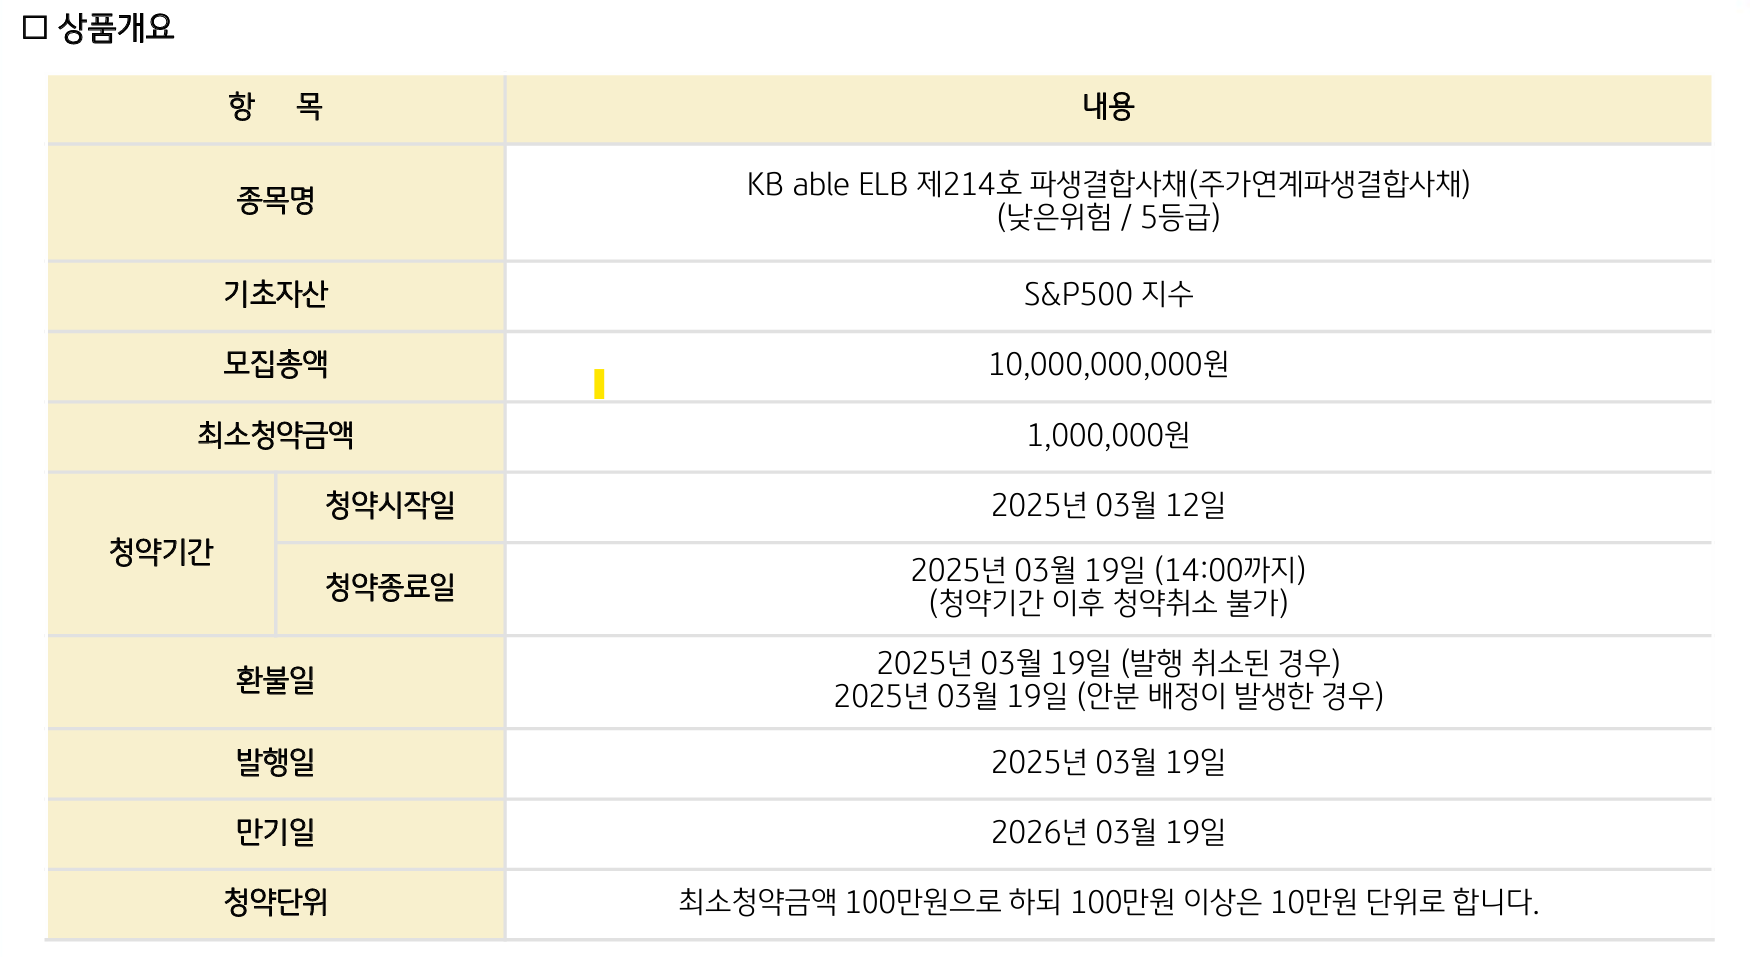
\includegraphics{image/elb1.png}


\includegraphics{image/elb2.png}

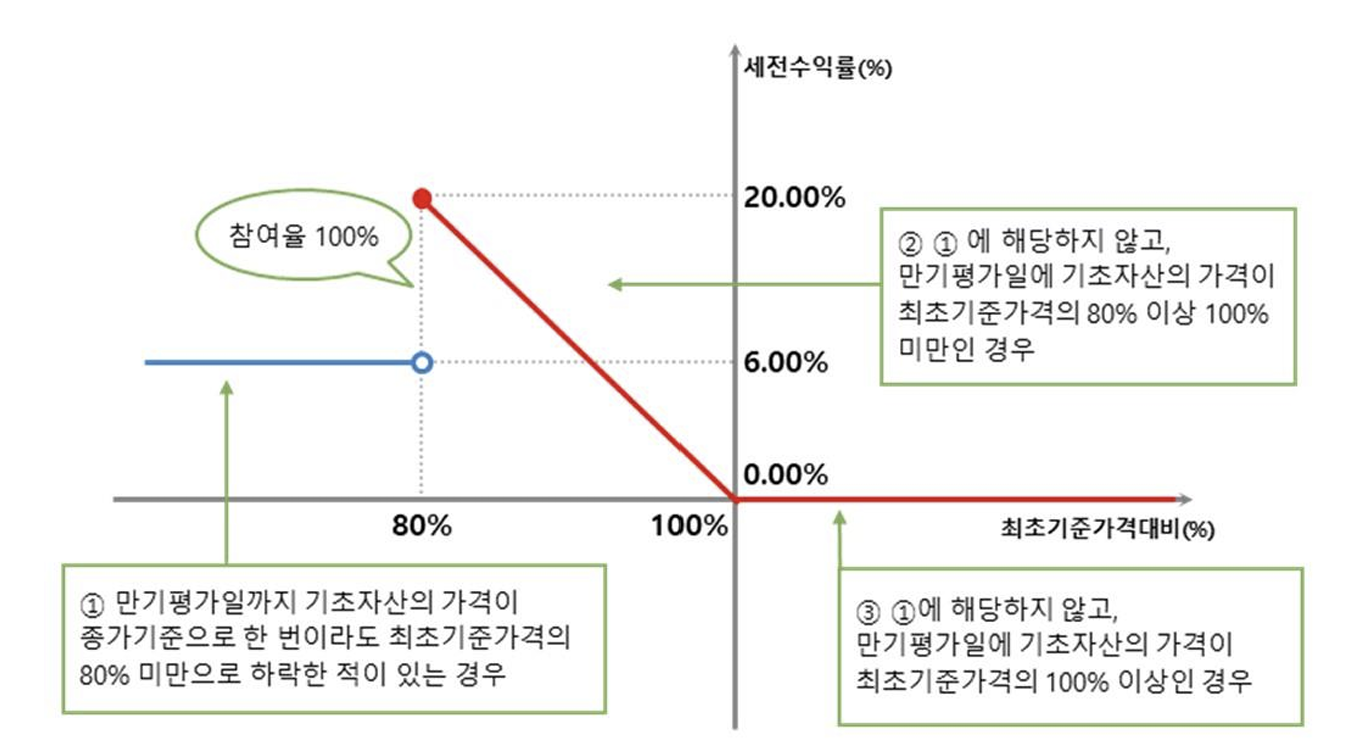
\includegraphics{image/elb3.png}

이는 \textbf{배리어옵션}의 한 종류로, 만기까지 한번이라도 배리어(20\%)
밑으로 하락하는 경우가 존재하면 옵션 권리가
사라지고(\textbf{Down-and-Out}), 대신 6\%의 rebate를 지급하는
구조입니다.

\section*{2. 평가}\label{uxd3c9uxac00}
\addcontentsline{toc}{section}{2. 평가}

\markright{2. 평가}

\subsection*{평가 개요}\label{uxd3c9uxac00-uxac1cuxc694}
\addcontentsline{toc}{subsection}{평가 개요}

평가는 몬테카를로 시뮬레이션을 이용할 계획이며, Numerix pricer와 동일한
2025-4-29일을 기준으로 pricing하도록 하겠습니다.

배리어옵션 평가를 위한 parameter는 아래와 같이 정리하였습니다.

\begin{itemize}
\tightlist
\item
  \(S_0\) : S\&P500지수의 최초기준가격평가일('25.3.19) 종가 (5,675.29pt)
\item
  \(S_1\) : S\&P500지수의 평가일('25.4.29) 종가 (5,560.83pt)
\item
  \(K\) : Down-and-out put options 행사가격(=\(S_0\times 100\%\))
\item
  \(B\) : Down-and-out put options 배리어가격(=\(S_0\times 80\%\))
\item
  \(r\) : 무위험이자율(=3\% 가정)
\item
  \(q\) : S\&P500 배당수익률(=0\% 가정정)
\item
  \(\sigma\) : 기초자산 변동성(=20\% 가정)
\item
  \(T_1\) : 잔존만기(=324/365)
\item
  \(T_2\) : 배리어옵션 평가대상만기(=321/365)
\item
  \(n\) : 몬테카를로 시뮬레이션 시행횟수
\item
  \(m\) : 시뮬레이션 경로 분할 갯수(거래일별, 220)
\item
  \(rebate\) : 배리어옵션 Knock-out 시 지급하는 쿠폰(=6\%)
\end{itemize}

\begin{tcolorbox}[enhanced jigsaw, bottomtitle=1mm, breakable, coltitle=black, opacityback=0, titlerule=0mm, left=2mm, colbacktitle=quarto-callout-note-color!10!white, toptitle=1mm, colframe=quarto-callout-note-color-frame, bottomrule=.15mm, opacitybacktitle=0.6, leftrule=.75mm, title=\textcolor{quarto-callout-note-color}{\faInfo}\hspace{0.5em}{파라미터 결정 근거}, arc=.35mm, toprule=.15mm, rightrule=.15mm, colback=white]

상품 평가를 위한 파라미터의 산정 근거는 아래와 같습니다.

\begin{verbatim}
- 기초자산가격, 행사가격, 배리어가격, 만기 등 : 상품 개요에서 확인

- 무위험이자율 : 미국에서는 SOFR, USD-libor, FFR 등이 널리 사용되며, Swap rate 등을 활용해 term-structure를 구성하는 것이 가장 정밀한 방법입니다. 분석의 단순화를 위해 3%로 가정하였습니다.
- S&P500 배당수익률 : 과거 배당이 유지된다고 가정하거나, 별도의 모델링을 통해 기간구조를 구성하는 것이 가장 정밀한 방법입니다. 분석의 단순화를 위해 배당이 없다고 가정하였습니다.
- 평가대상만기 : 명목 만기는 1년이나, 만기평가일에 옵션 payoff가 결정되므로, 3거래일을 차감한 값을 활용하였습니다.
- 기초자산 변동성 : 시장가격을 활용한 내재변동성을 이용하였으며, Local Vol 등을 통해 Surface를 구성하여 시뮬레이션 하는 것이 가장 정밀한 방법입니다. 다만, 분석의 단순화를 위해 20%로 가정하였습니다.
- 경로 분할 갯수 : Lookback period의 간격이 1일이므로 거래일수로 분할하였습니다.
\end{verbatim}

거래일은 NYSE를 기준으로 산출하였고, 데이터는 \texttt{yahoo\ finance},
\texttt{cme}, \texttt{cboe}를 참고하였습니다.

\begin{Shaded}
\begin{Highlighting}[]
\ImportTok{import}\NormalTok{ pandas\_market\_calendars }\ImportTok{as}\NormalTok{ mcal}
\ImportTok{from}\NormalTok{ datetime }\ImportTok{import}\NormalTok{ date}

\NormalTok{exp\_dd }\OperatorTok{=}\NormalTok{ date(}\DecValTok{2026}\NormalTok{, }\DecValTok{3}\NormalTok{, }\DecValTok{19}\NormalTok{)}\OperatorTok{;}\NormalTok{ strt\_dd }\OperatorTok{=}\NormalTok{ date(}\DecValTok{2025}\NormalTok{, }\DecValTok{4}\NormalTok{, }\DecValTok{29}\NormalTok{)}\OperatorTok{;}
\NormalTok{exptime }\OperatorTok{=}\NormalTok{ (exp\_dd }\OperatorTok{{-}}\NormalTok{ strt\_dd).days}

\NormalTok{strt }\OperatorTok{=} \StringTok{\textquotesingle{}2025{-}04{-}30\textquotesingle{}}\OperatorTok{;}\NormalTok{ end}\OperatorTok{=}\StringTok{\textquotesingle{}2026{-}03{-}16\textquotesingle{}}\OperatorTok{;}\NormalTok{ nyse }\OperatorTok{=}\NormalTok{ mcal.get\_calendar(}\StringTok{\textquotesingle{}NYSE\textquotesingle{}}\NormalTok{)}\OperatorTok{;}
\NormalTok{timesteps }\OperatorTok{=}\NormalTok{ nyse.valid\_days(start\_date}\OperatorTok{=}\NormalTok{strt, end\_date}\OperatorTok{=}\NormalTok{end)}

\BuiltInTok{print}\NormalTok{(}\StringTok{"Day to maturity is :"}\NormalTok{,exptime)}
\BuiltInTok{print}\NormalTok{(}\StringTok{"Number of trading day(timestep) is :"}\NormalTok{,}\BuiltInTok{len}\NormalTok{(timesteps))}
\end{Highlighting}
\end{Shaded}

\begin{verbatim}
Day to maturity is : 324
Number of trading day(timestep) is : 220
\end{verbatim}

\end{tcolorbox}

\subsection*{평가 알고리즘}\label{uxd3c9uxac00-uxc54cuxace0uxb9acuxc998}
\addcontentsline{toc}{subsection}{평가 알고리즘}

기초자산인 \textbf{S\&P500 지수가 GBM을 따른다는 가정} 하에 정규난수를
이용하여 만기평가일까지의 주가흐름을 시뮬레이션할 계획이며, 알고리즘은
아래와 같습니다.

\begin{enumerate}
\def\labelenumi{(\arabic{enumi})}
\tightlist
\item
  현재 주가(\(S_0\))와 만기(\(T_2\)), 변동성(\(\sigma\)),
  기대수익률(\(\mu=r-d\))를 통해 GBM을 구성하고, Euler's
  discretization을 통해 248거래일마다 종가를 생성

  \begin{itemize}
  \tightlist
  \item
    먼저, 평가대상만기일의 종가를 n개 생성(Stratified sampling, Moment
    matching, Antithetic variate를 활용하여 균질한 분포를 구현)
  \item
    각 n개의 종가마다, 그 경로의 247(총 (m-1)*n)개의 난수를
    생성(Antithetic variate 적용)하고, brownian bridge 방법을 통해
    오일러 이산화를 구현
  \end{itemize}
\item
  각 경로마다 Knock 여부와 내재가치를 고려하여 배리어옵션의 payoff와
  npv를 결정

  \begin{itemize}
  \tightlist
  \item
    Knock-out 발생 : 명목금액의 6\%의 rebate를 지급받음
  \item
    Knock-out 미발생 : 평가만기일 종가에 따라 풋옵션 내재가치를 지급받음
  \item
    각 payoff를 잔존만기(\(T_1\))에 대해 할인하여 npv를 산출
  \end{itemize}
\item
  이에 따라 산출된 npv를 산술평균을 통해 배리어옵션(ELB)의 공정가치를
  산출
\end{enumerate}

\subsection*{알고리즘 구현 (Python
code)}\label{uxc54cuxace0uxb9acuxc998-uxad6cuxd604-python-code}
\addcontentsline{toc}{subsection}{알고리즘 구현 (Python code)}

알고리즘을 Python 코드로 구현하였으며, Down-out Put option 가격과 GBM을
활용한 기초자산의 경로를 반환하는 함수로 작성하였습니다.

\begin{Shaded}
\begin{Highlighting}[]
\ImportTok{import}\NormalTok{ numpy }\ImportTok{as}\NormalTok{ np}
\ImportTok{import}\NormalTok{ scipy.stats }\ImportTok{as}\NormalTok{ sst}

\KeywordTok{def}\NormalTok{ DownAndOutPut\_Price(s, k, r, q, t, sigma, n, b, m, rebate):}
    \CommentTok{\# Set parameters}
\NormalTok{    dt }\OperatorTok{=}\NormalTok{ t}\OperatorTok{/}\NormalTok{m}
\NormalTok{    dts }\OperatorTok{=}\NormalTok{ np.arange(dt, t}\OperatorTok{+}\NormalTok{dt, dt)}

    \CommentTok{\# (1) Stratified sampling, z\_t makes price at T \& z makes brownian bridge}
\NormalTok{    z\_t }\OperatorTok{=}\NormalTok{ sst.norm.ppf((np.arange(n) }\OperatorTok{+}\NormalTok{ np.random.uniform(}\DecValTok{0}\NormalTok{,}\DecValTok{1}\NormalTok{,n)) }\OperatorTok{/}\NormalTok{ n)}
\NormalTok{    z }\OperatorTok{=}\NormalTok{ np.random.randn(n,m)}
    \CommentTok{\# (2) Moment matching in z\_t}
\NormalTok{    z\_t }\OperatorTok{=}\NormalTok{ np.where(n}\OperatorTok{\textgreater{}=}\DecValTok{100}\NormalTok{, (z\_t }\OperatorTok{{-}}\NormalTok{ z\_t.mean()) }\OperatorTok{/}\NormalTok{ z\_t.std(ddof}\OperatorTok{=}\DecValTok{1}\NormalTok{), z\_t }\OperatorTok{{-}}\NormalTok{ z\_t.mean())}
    \CommentTok{\# (3) Antithetic variate}
\NormalTok{    z\_t, z }\OperatorTok{=}\NormalTok{ np.concatenate([z\_t, }\OperatorTok{{-}}\NormalTok{z\_t], axis}\OperatorTok{=}\DecValTok{0}\NormalTok{), np.concatenate([z, }\OperatorTok{{-}}\NormalTok{z], axis}\OperatorTok{=}\DecValTok{0}\NormalTok{)}

    \CommentTok{\# Generate underlying paths using brownian bridge}
\NormalTok{    w\_t, w }\OperatorTok{=}\NormalTok{ z\_t }\OperatorTok{*}\NormalTok{ np.sqrt(t), z.cumsum(axis}\OperatorTok{=}\DecValTok{1}\NormalTok{) }\OperatorTok{*}\NormalTok{ np.sqrt(dt) }\CommentTok{\# winner process}
\NormalTok{    bridge }\OperatorTok{=}\NormalTok{ dts }\OperatorTok{*}\NormalTok{ ((w\_t}\OperatorTok{{-}}\NormalTok{ w[:,}\OperatorTok{{-}}\DecValTok{1}\NormalTok{]).reshape(}\BuiltInTok{len}\NormalTok{(w),}\DecValTok{1}\NormalTok{) }\OperatorTok{+}\NormalTok{ w }\OperatorTok{/}\NormalTok{ dts) }\CommentTok{\# brownian bridge}
\NormalTok{    paths }\OperatorTok{=}\NormalTok{ s}\OperatorTok{*}\NormalTok{np.exp((r}\OperatorTok{{-}}\NormalTok{q}\OperatorTok{{-}}\FloatTok{0.5}\OperatorTok{*}\NormalTok{sigma}\OperatorTok{**}\DecValTok{2}\NormalTok{)}\OperatorTok{*}\NormalTok{dts }\OperatorTok{+}\NormalTok{ sigma}\OperatorTok{*}\NormalTok{bridge) }\CommentTok{\# underlying path}
    \CommentTok{\# Determine Knock{-}out}
\NormalTok{    knock }\OperatorTok{=}\NormalTok{ paths.}\BuiltInTok{min}\NormalTok{(axis}\OperatorTok{=}\DecValTok{1}\NormalTok{) }\OperatorTok{\textless{}}\NormalTok{ b }\CommentTok{\# knock{-}out = 1 else 0}
\NormalTok{    barrier\_flag }\OperatorTok{=} \OperatorTok{\textasciitilde{}}\NormalTok{knock}

    \CommentTok{\# Caculate options payoff}
\NormalTok{    plain\_npv }\OperatorTok{=}\NormalTok{ np.maximum(k}\OperatorTok{{-}}\NormalTok{paths[:,}\OperatorTok{{-}}\DecValTok{1}\NormalTok{], }\DecValTok{0}\NormalTok{) }\OperatorTok{*}\NormalTok{ np.exp(}\OperatorTok{{-}}\NormalTok{r}\OperatorTok{*}\NormalTok{t)}
\NormalTok{    barrier\_npv }\OperatorTok{=}\NormalTok{ barrier\_flag }\OperatorTok{*}\NormalTok{ plain\_npv }\OperatorTok{+}\NormalTok{ knock }\OperatorTok{*}\NormalTok{ rebate }\OperatorTok{*}\NormalTok{ np.exp(}\OperatorTok{{-}}\NormalTok{r}\OperatorTok{*}\NormalTok{t)}
\NormalTok{    barrier\_price }\OperatorTok{=}\NormalTok{ barrier\_npv.mean()}

    \ControlFlowTok{return}\NormalTok{ barrier\_price, paths}
\end{Highlighting}
\end{Shaded}

\section*{3. 평가 결과 및 비교(Numerix
Pricer)}\label{uxd3c9uxac00-uxacb0uxacfc-uxbc0f-uxbe44uxad50numerix-pricer}
\addcontentsline{toc}{section}{3. 평가 결과 및 비교(Numerix Pricer)}

\markright{3. 평가 결과 및 비교(Numerix Pricer)}

\subsection*{배리어옵션 가격 및 기초자산
경로}\label{uxbc30uxb9acuxc5b4uxc635uxc158-uxac00uxaca9-uxbc0f-uxae30uxcd08uxc790uxc0b0-uxacbduxb85c}
\addcontentsline{toc}{subsection}{배리어옵션 가격 및 기초자산 경로}

상술한 2025-4-29일의 기준 파라미터를 이용하여 배리어옵션의 가격을
평가해보았습니다.

가격은 명목금액 \textbf{10,000원을 기준으로 약 365원이며, 수익률로
환산할 때 약 3.65\%}입니다.

시뮬레이션 횟수는 10만번 기준으로, 난수에 따라 편차가 약
1\textasciitilde2원 존재하였습니다.

\begin{Shaded}
\begin{Highlighting}[]
\NormalTok{s0 }\OperatorTok{=} \FloatTok{5675.29}\OperatorTok{;}\NormalTok{ s1 }\OperatorTok{=} \FloatTok{5560.83}
\NormalTok{k }\OperatorTok{=}\NormalTok{ s0}\OperatorTok{;}\NormalTok{ b }\OperatorTok{=} \FloatTok{0.8} \OperatorTok{*}\NormalTok{ s0}
\NormalTok{r }\OperatorTok{=} \FloatTok{0.03}\OperatorTok{;}\NormalTok{ q }\OperatorTok{=} \DecValTok{0}\OperatorTok{;}\NormalTok{ sigma }\OperatorTok{=} \FloatTok{0.2}\OperatorTok{;}\NormalTok{ rebate }\OperatorTok{=} \FloatTok{0.06} \OperatorTok{*}\NormalTok{ s0}
\NormalTok{t1 }\OperatorTok{=}\NormalTok{ exptime }\OperatorTok{/} \DecValTok{365}\OperatorTok{;}\NormalTok{ t2 }\OperatorTok{=}\NormalTok{ (exptime}\OperatorTok{{-}}\DecValTok{3}\NormalTok{) }\OperatorTok{/} \DecValTok{365}
\NormalTok{n }\OperatorTok{=} \DecValTok{100000}\OperatorTok{;}\NormalTok{ m }\OperatorTok{=} \BuiltInTok{len}\NormalTok{(timesteps)}
\NormalTok{notional }\OperatorTok{=} \DecValTok{10000}
\NormalTok{nxprice }\OperatorTok{=} \FloatTok{366.8977875}

\NormalTok{price, GBMpath }\OperatorTok{=}\NormalTok{ DownAndOutPut\_Price(s1, k, r, q, t2, sigma, n, b, m, rebate)}
\NormalTok{price }\OperatorTok{=}\NormalTok{ price }\OperatorTok{*}\NormalTok{ np.exp(r}\OperatorTok{*}\NormalTok{(t2}\OperatorTok{{-}}\NormalTok{t1)) }\OperatorTok{/}\NormalTok{ s0 }\OperatorTok{*}\NormalTok{ notional }\CommentTok{\# Convert discount \& notional}
\BuiltInTok{print}\NormalTok{(}\SpecialStringTok{f"Down{-}and{-}Out Barrier Put options price is : }\SpecialCharTok{\{}\NormalTok{price}\SpecialCharTok{:.4f\}}\SpecialStringTok{"}\NormalTok{)}
\end{Highlighting}
\end{Shaded}

\begin{verbatim}
Down-and-Out Barrier Put options price is : 364.9572
\end{verbatim}

시뮬레이션에 이용된 기초자산의 경로를 시각화한 결과입니다.

계층화, 표준화 등 분산감소기법이 잘 적용되어 \textbf{만기시점의
Lognormal dist. 형태}가 잘 나타난 것을 볼 수 있으며, 시뮬레이션 중
배리어가격 밑으로 하락한 경우가 발생한 \textbf{Knock-out의 비율은 약
22.7\%}로 나타났습니다.

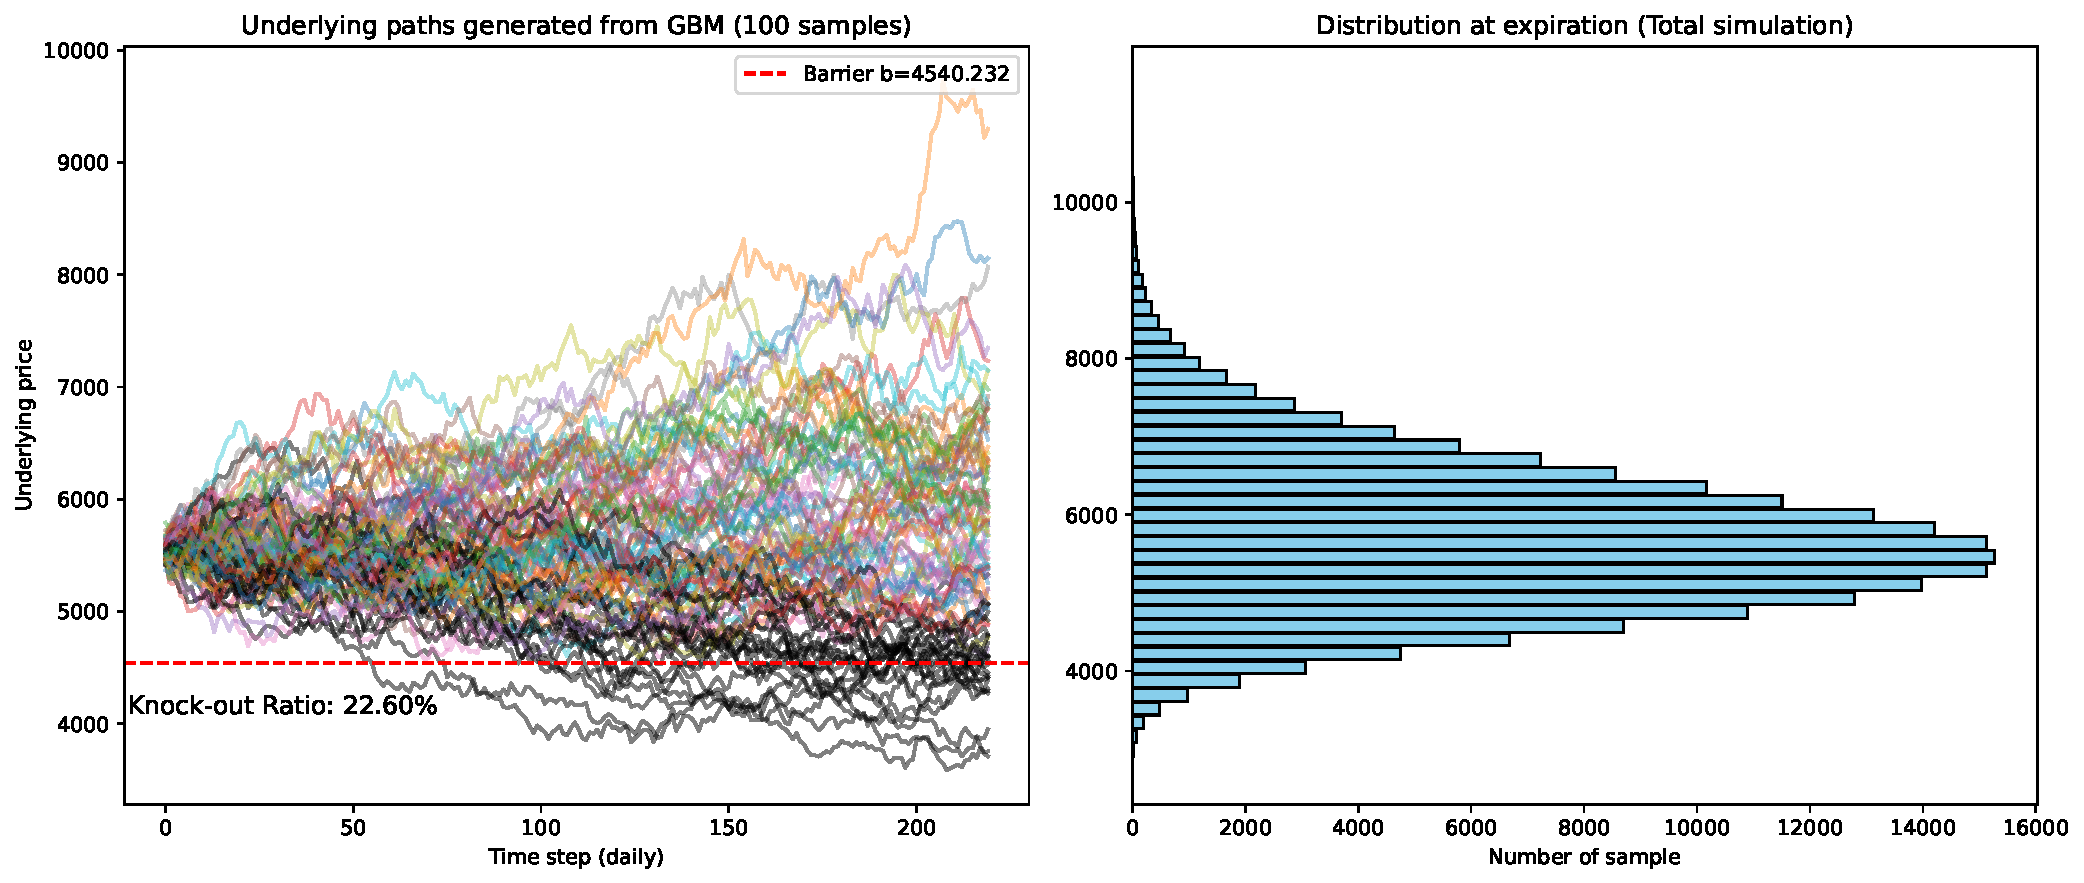
\includegraphics{otc_hw_files/figure-pdf/cell-5-output-1.pdf}

\subsection*{Numerix Pricer와
비교}\label{numerix-priceruxc640-uxbe44uxad50}
\addcontentsline{toc}{subsection}{Numerix Pricer와 비교}

파이썬에서 구현한 환경과 최대한 유사하도록 기존 Numerix pricer에서
무위험이자율 커브 및 변동성 곡면을 각각 3\%, 20\% 단일값으로
수정하였으며, 기초자산의 가격도 2025-4-29일 종가인 5560.83pt로
수정하였습니다.

이에 따라 수정된 Numerix를 이용한 배리어옵션 가격은 약 366.9원(3.67\%)로
산출되었습니다.

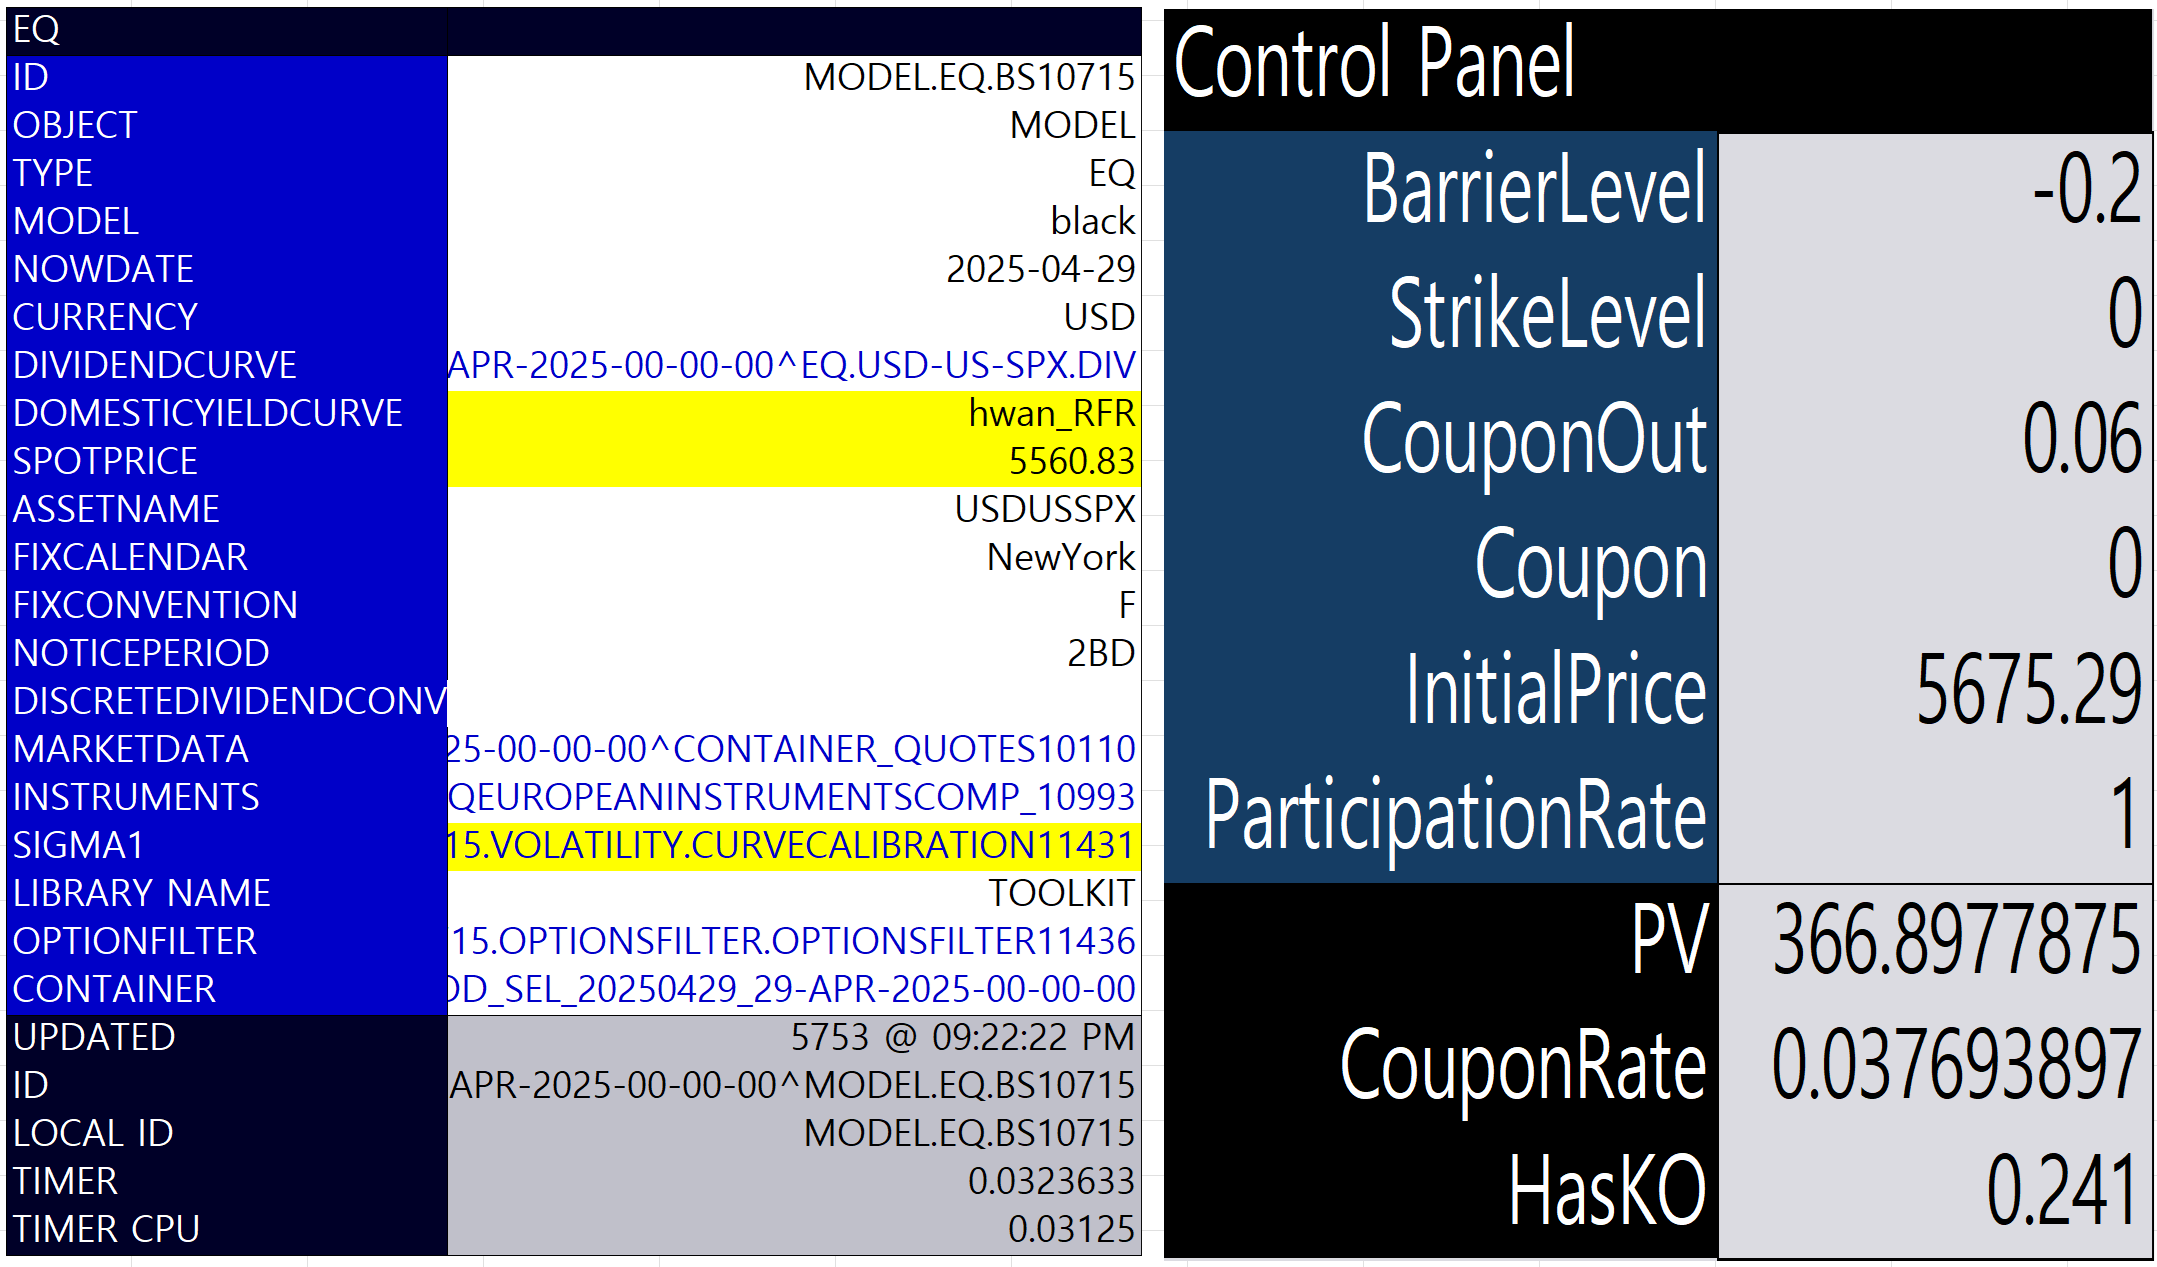
\includegraphics{image/numerix_pricer.png}

\textbf{두 가격간의 괴리율은 1\% 미만 수준으로, 상당히 유사}한 것을
확인할 수 있었습니다.

Knock-out 비율도 Numerix에서 약 24\%로 기존의 약 23\%와 매우
유사하였습니다.

\begin{verbatim}
Difference ratio is : 0.0053
\end{verbatim}

\section*{4. 소결}\label{uxc18cuxacb0}
\addcontentsline{toc}{section}{4. 소결}

\markright{4. 소결}

\textbf{Down-and-out put options 형태의 ELB}를 기본적인 Black-sholes
공식을 기반으로 \textbf{두가지 방식으로 평가}하였습니다.

\begin{enumerate}
\def\labelenumi{\arabic{enumi}.}
\tightlist
\item
  Montecarlo Simulation : 기초자산의 가격경로를 생성하여 베리어옵션의
  payoff를 평가
\item
  Numerix pricer : Numerix에서 제공하는 Black 모델 및 Kernel object를
  이용하여 가격 평가
\end{enumerate}

그 결과, \textbf{두 방식에서 매우 유사한 결과}를 얻을 수 있었으며
Knock-out 비율의 차이도 미미하여 기초자산의 가격경로의 생성방법이
비슷하다는 것을 유추할 수 있었습니다.

\textbf{Numerix pricer}에서는 기초적인 MCS방법 뿐만아니라,
이자율/배당/변동성 등 \textbf{기간구조를 가지는 변수}들을 object로
형성하고 이를 \textbf{쉽게 가격평가에 적용}할 수 있는 장점이 있었습니다.
그러나, \textbf{파이썬 환경}에서 이를 적용하기 위해서는 모든 난수생성 및
경로생성에 개입하여 Stocastic한 이자율/변동성 등 변수들을 일일히
적용해야하므로, \textbf{계산자원이 급격히 증가할 것으로 예상}됩니다.

본 분석의 \textbf{한계점}은 \textbf{다양한 변수조건에서의 검증이
생략}되어있다는 점 입니다. 상술한 기간구조를 반영하지 못한 부분
뿐만아니라, 분석에서 다루지는 않았으나 \textbf{시장변동성이 커지는
상황}에서 MCS와 Numerix pricer의 \textbf{괴리율이 증가하는 경향}을
보였습니다.

부가적으로, QuantLib library를 이용하여 동일한 배리어옵션의
\textbf{Analytic price를 산출}해본 결과, \textbf{MCS 및 Numerix 방식과는
큰 차이}가 있었습니다. 이는 Analytic price를 산출할때 \textbf{연속시간을
가정}하므로, 실제 종가로만 판단하는 daily 시간간격대비 \textbf{Knock-out
비율이 높아져 옵션 가격을 저평가}하는 것으로 추정됩니다.

\begin{tcolorbox}[enhanced jigsaw, bottomtitle=1mm, breakable, coltitle=black, opacityback=0, titlerule=0mm, left=2mm, colbacktitle=quarto-callout-tip-color!10!white, toptitle=1mm, colframe=quarto-callout-tip-color-frame, bottomrule=.15mm, opacitybacktitle=0.6, leftrule=.75mm, title=\textcolor{quarto-callout-tip-color}{\faLightbulb}\hspace{0.5em}{QuantLib을 이용한 배리어옵션 평가}, arc=.35mm, toprule=.15mm, rightrule=.15mm, colback=white]

\begin{Shaded}
\begin{Highlighting}[]
\ImportTok{import}\NormalTok{ QuantLib }\ImportTok{as}\NormalTok{ ql}

\NormalTok{today }\OperatorTok{=}\NormalTok{ ql.Date(}\DecValTok{29}\NormalTok{, }\DecValTok{4}\NormalTok{, }\DecValTok{2025}\NormalTok{)}
\NormalTok{maturity }\OperatorTok{=}\NormalTok{ ql.Date(}\DecValTok{16}\NormalTok{, }\DecValTok{3}\NormalTok{, }\DecValTok{2026}\NormalTok{)}
\NormalTok{ql.Settings.instance().evaluationDate }\OperatorTok{=}\NormalTok{ today}

\NormalTok{payoff }\OperatorTok{=}\NormalTok{ ql.PlainVanillaPayoff(ql.Option.Put, k)}
\NormalTok{euExercise }\OperatorTok{=}\NormalTok{ ql.EuropeanExercise(maturity)}
\NormalTok{barrierOption }\OperatorTok{=}\NormalTok{ ql.BarrierOption(ql.Barrier.DownOut, b, rebate, payoff, euExercise)}

\NormalTok{spotHandle }\OperatorTok{=}\NormalTok{ ql.QuoteHandle(ql.SimpleQuote(s1))}
\NormalTok{flatRateTs }\OperatorTok{=}\NormalTok{ ql.YieldTermStructureHandle(ql.FlatForward(today, r, ql.Actual365Fixed()))}
\NormalTok{flatVolTs }\OperatorTok{=}\NormalTok{ ql.BlackVolTermStructureHandle(ql.BlackConstantVol(today, ql.NullCalendar(), sigma, ql.Actual365Fixed()))}
\NormalTok{bsm }\OperatorTok{=}\NormalTok{ ql.BlackScholesProcess(spotHandle, flatRateTs, flatVolTs)}

\NormalTok{analyticBarrierEngine }\OperatorTok{=}\NormalTok{ ql.AnalyticBarrierEngine(bsm)}
\NormalTok{barrierOption.setPricingEngine(analyticBarrierEngine)}
\NormalTok{analytic\_price }\OperatorTok{=}\NormalTok{ barrierOption.NPV() }\OperatorTok{*}\NormalTok{ np.exp(r}\OperatorTok{*}\NormalTok{(t2}\OperatorTok{{-}}\NormalTok{t1)) }\OperatorTok{/}\NormalTok{ s0 }\OperatorTok{*}\NormalTok{ notional}

\BuiltInTok{print}\NormalTok{(}\SpecialStringTok{f"Analytic Price is : }\SpecialCharTok{\{}\NormalTok{analytic\_price}\SpecialCharTok{:.4f\}}\SpecialStringTok{"}\NormalTok{)}
\end{Highlighting}
\end{Shaded}

\begin{verbatim}
Analytic Price is : 357.1444
\end{verbatim}

\end{tcolorbox}

\part{금융윤리와 사회책임('25 봄)}

\chapter*{금융윤리와
사회책임}\label{uxae08uxc735uxc724uxb9acuxc640-uxc0acuxd68cuxcc45uxc784}
\addcontentsline{toc}{chapter}{금융윤리와 사회책임}

\markboth{금융윤리와 사회책임}{금융윤리와 사회책임}

\textbf{\emph{20249132 김형환}}

\section*{Standard 1 :
Professionalism}\label{standard-1-professionalism}
\addcontentsline{toc}{section}{Standard 1 : Professionalism}

\markright{Standard 1 : Professionalism}

\subsection*{A. 법규의 이해와 준수 (Knowledge of the
Law)}\label{a.-uxbc95uxaddcuxc758-uxc774uxd574uxc640-uxc900uxc218-knowledge-of-the-law}
\addcontentsline{toc}{subsection}{A. 법규의 이해와 준수 (Knowledge of
the Law)}


\includegraphics{image/ethic1A.png}

\subsubsection*{\texorpdfstring{\textbf{\emph{Assignment
1}}}{Assignment 1}}\label{assignment-1}
\addcontentsline{toc}{subsubsection}{\textbf{\emph{Assignment 1}}}

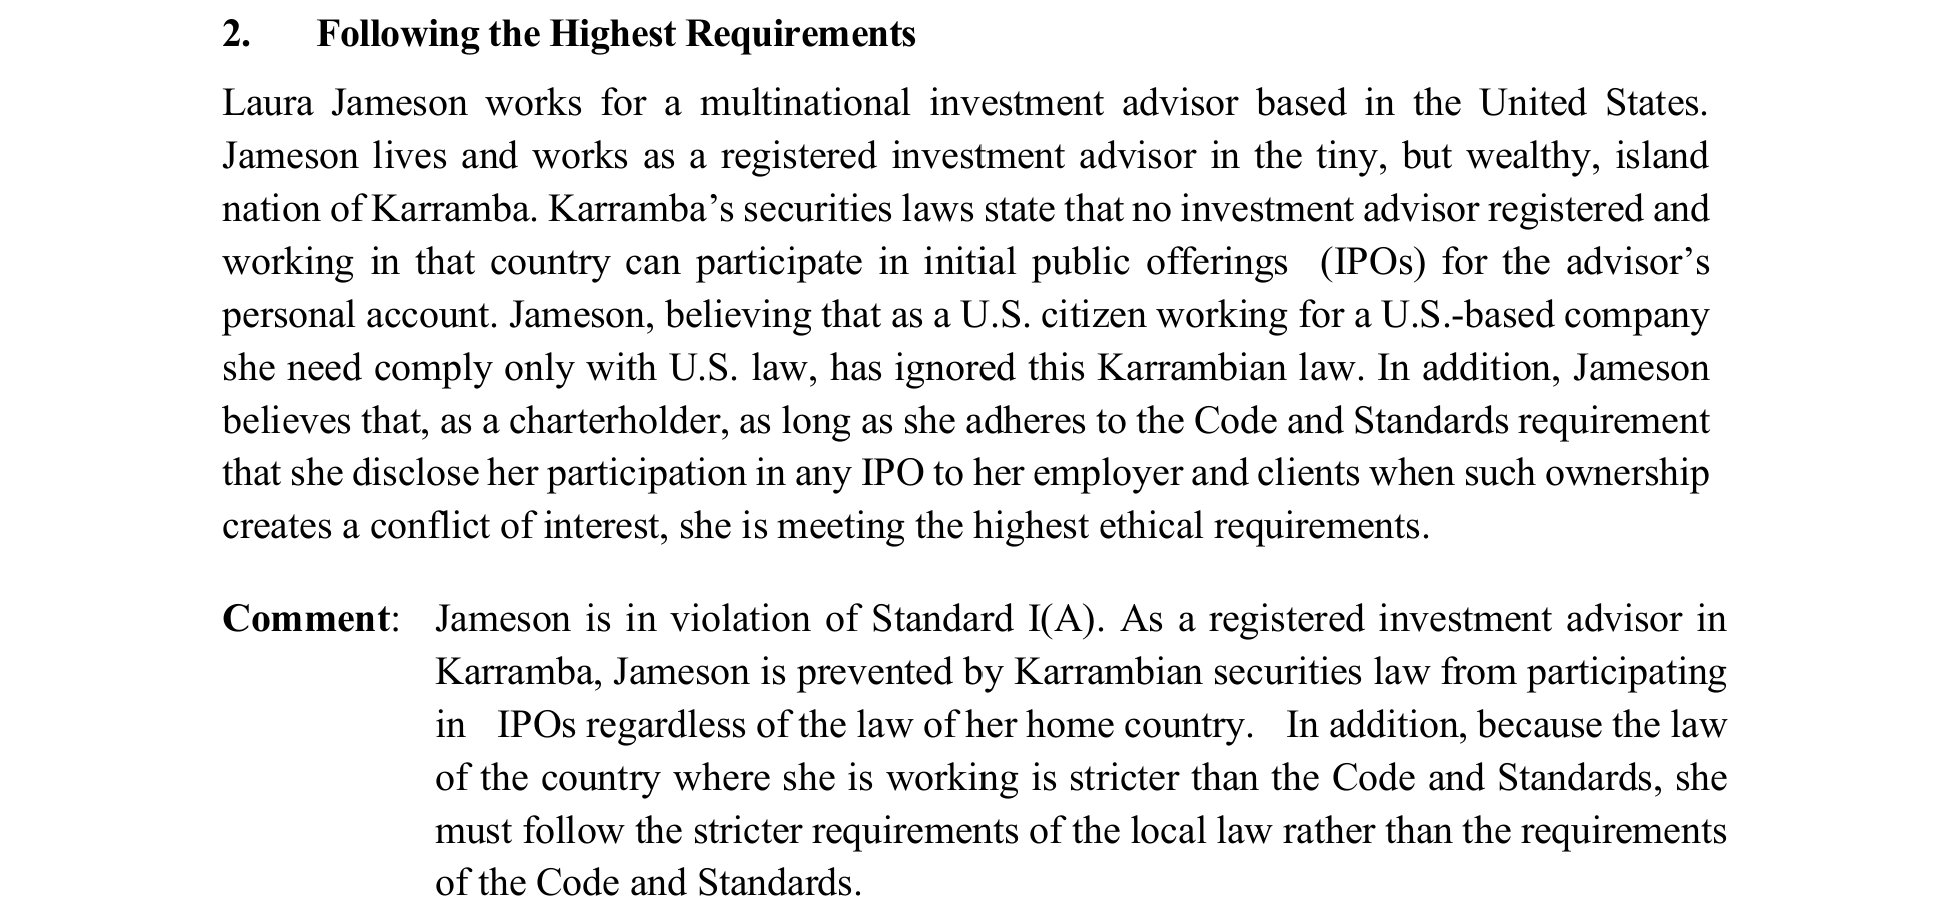
\includegraphics{image/ethic1.png}

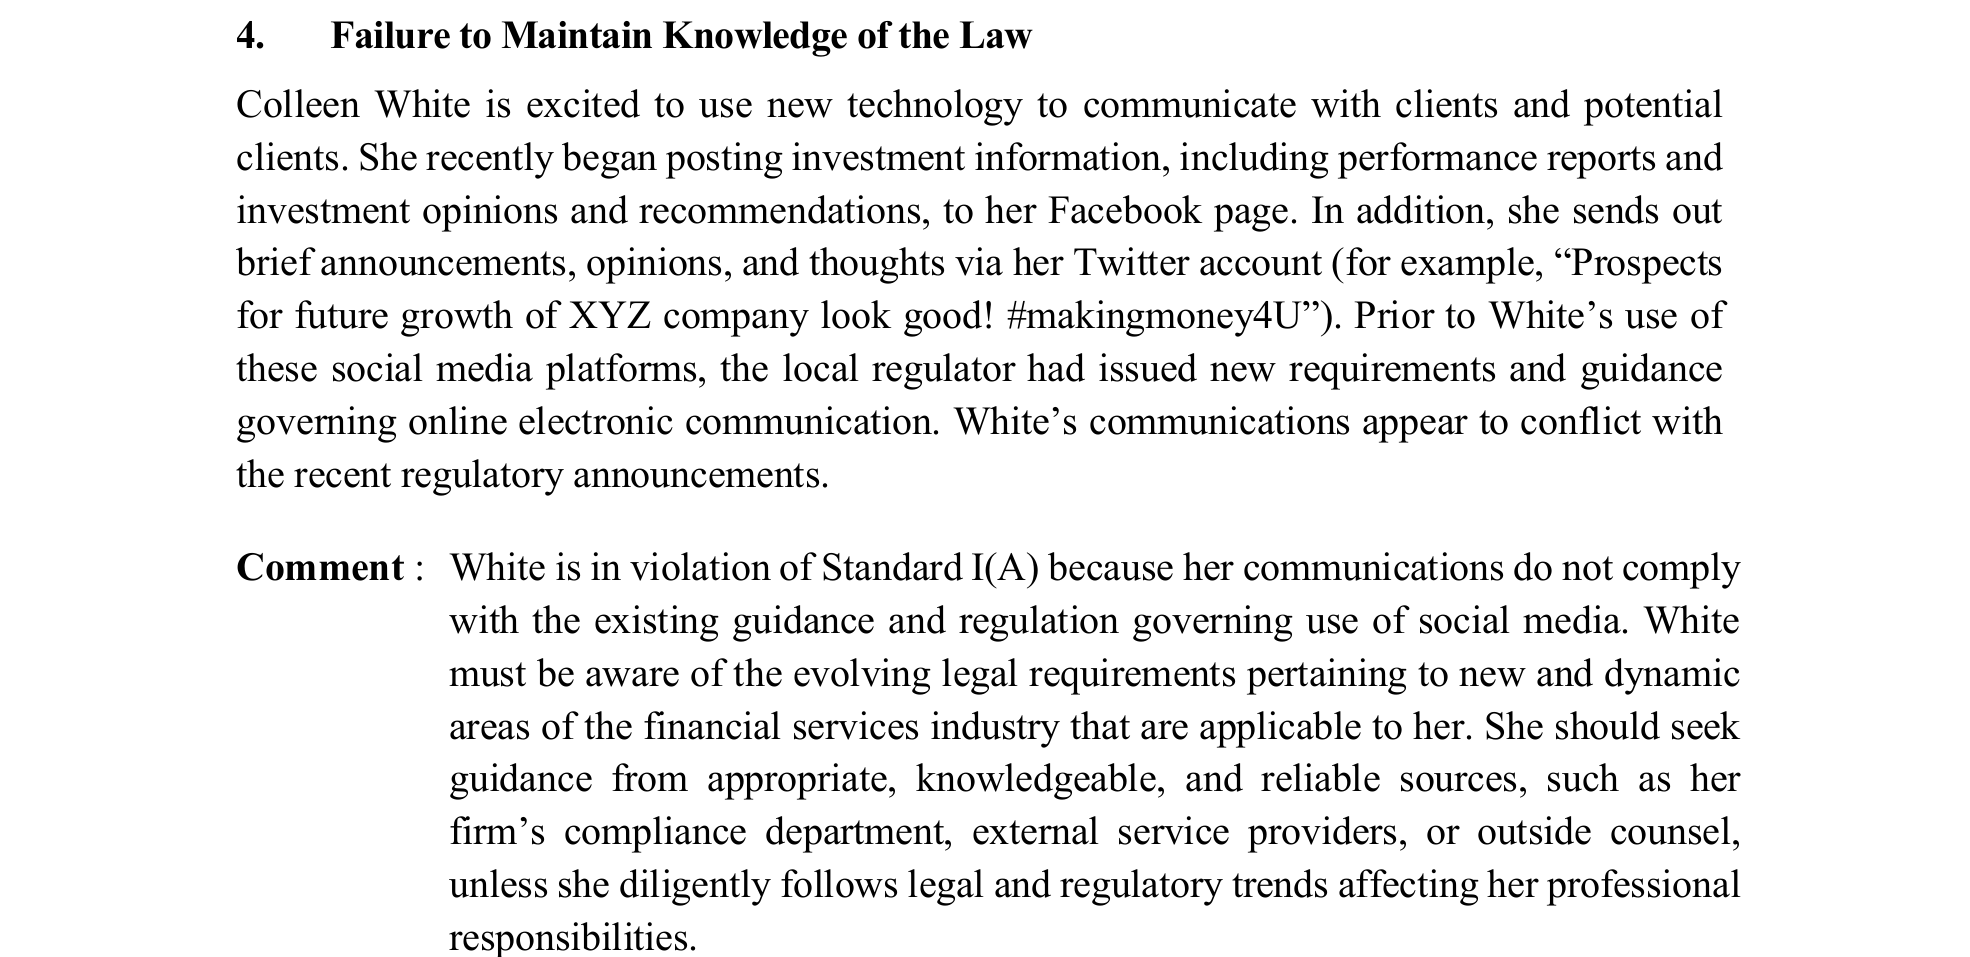
\includegraphics{image/ethic2.png}

\subsection*{C. 오해의 소지가 있는 표현 금지
(Misrepresentation)}\label{c.-uxc624uxd574uxc758-uxc18cuxc9c0uxac00-uxc788uxb294-uxd45cuxd604-uxae08uxc9c0-misrepresentation}
\addcontentsline{toc}{subsection}{C. 오해의 소지가 있는 표현 금지
(Misrepresentation)}

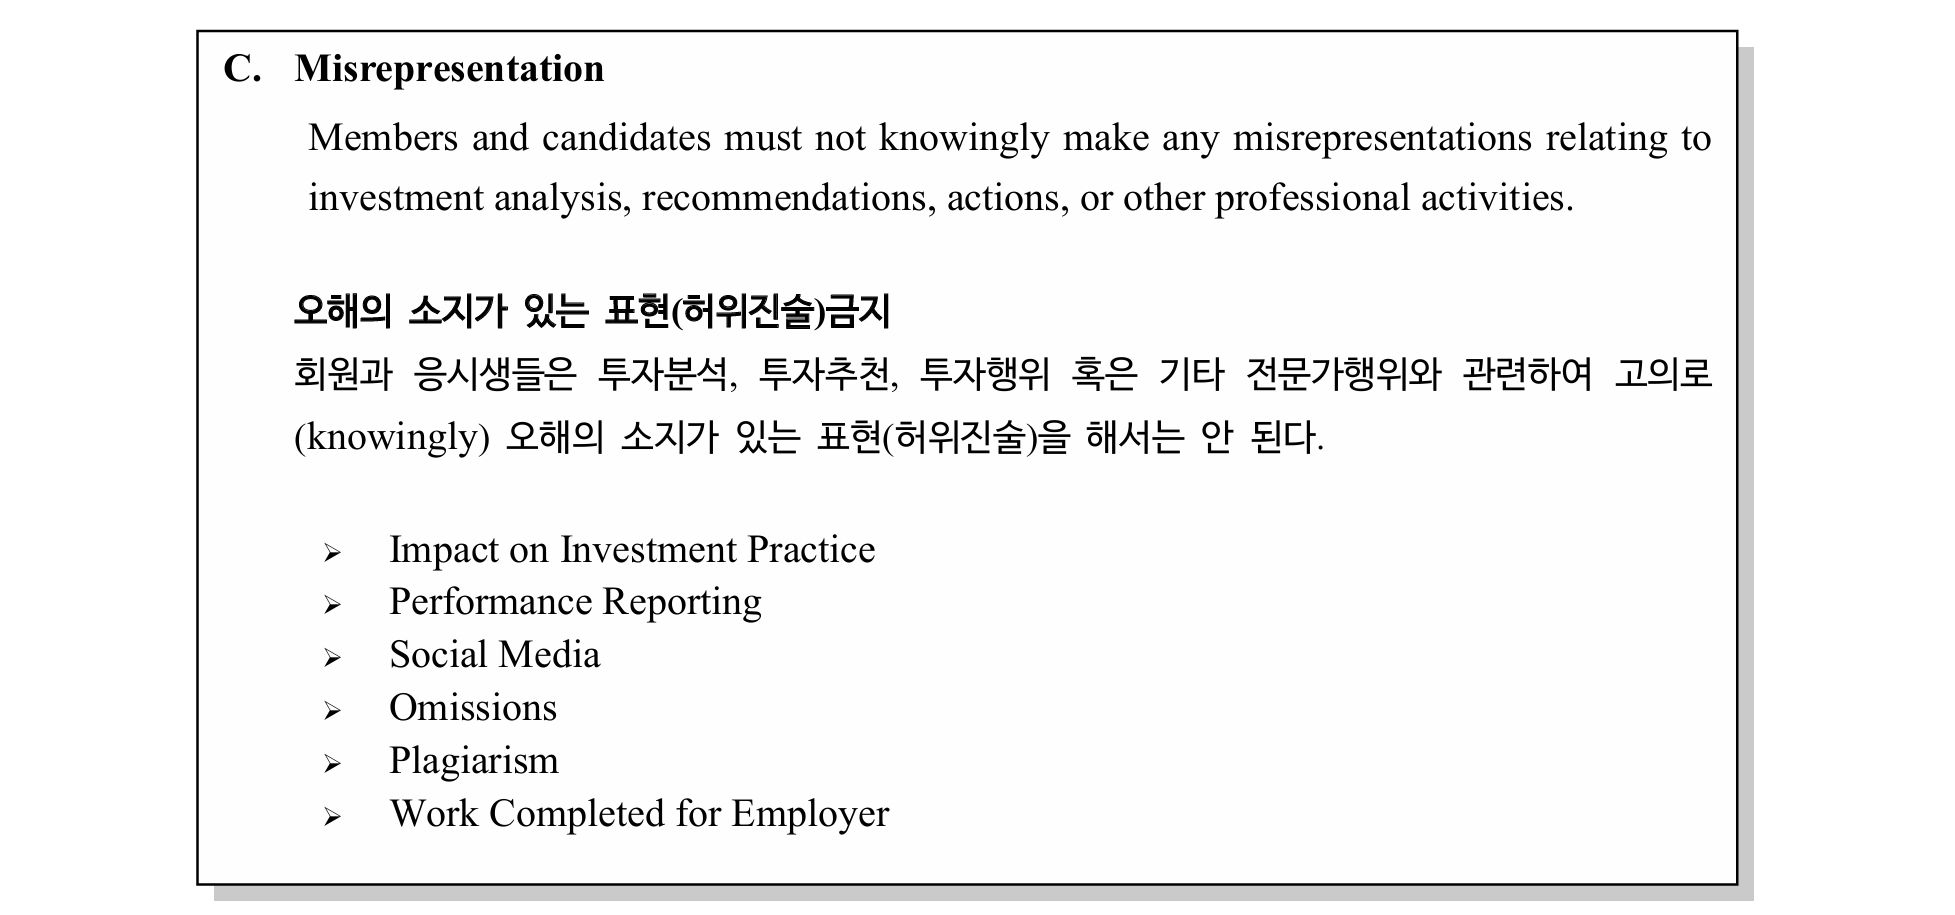
\includegraphics{image/ethic1C.png}

\subsubsection*{\texorpdfstring{\textbf{\emph{Assignment
1}}}{Assignment 1}}\label{assignment-1-1}
\addcontentsline{toc}{subsubsection}{\textbf{\emph{Assignment 1}}}


\includegraphics{image/ethic3.png}

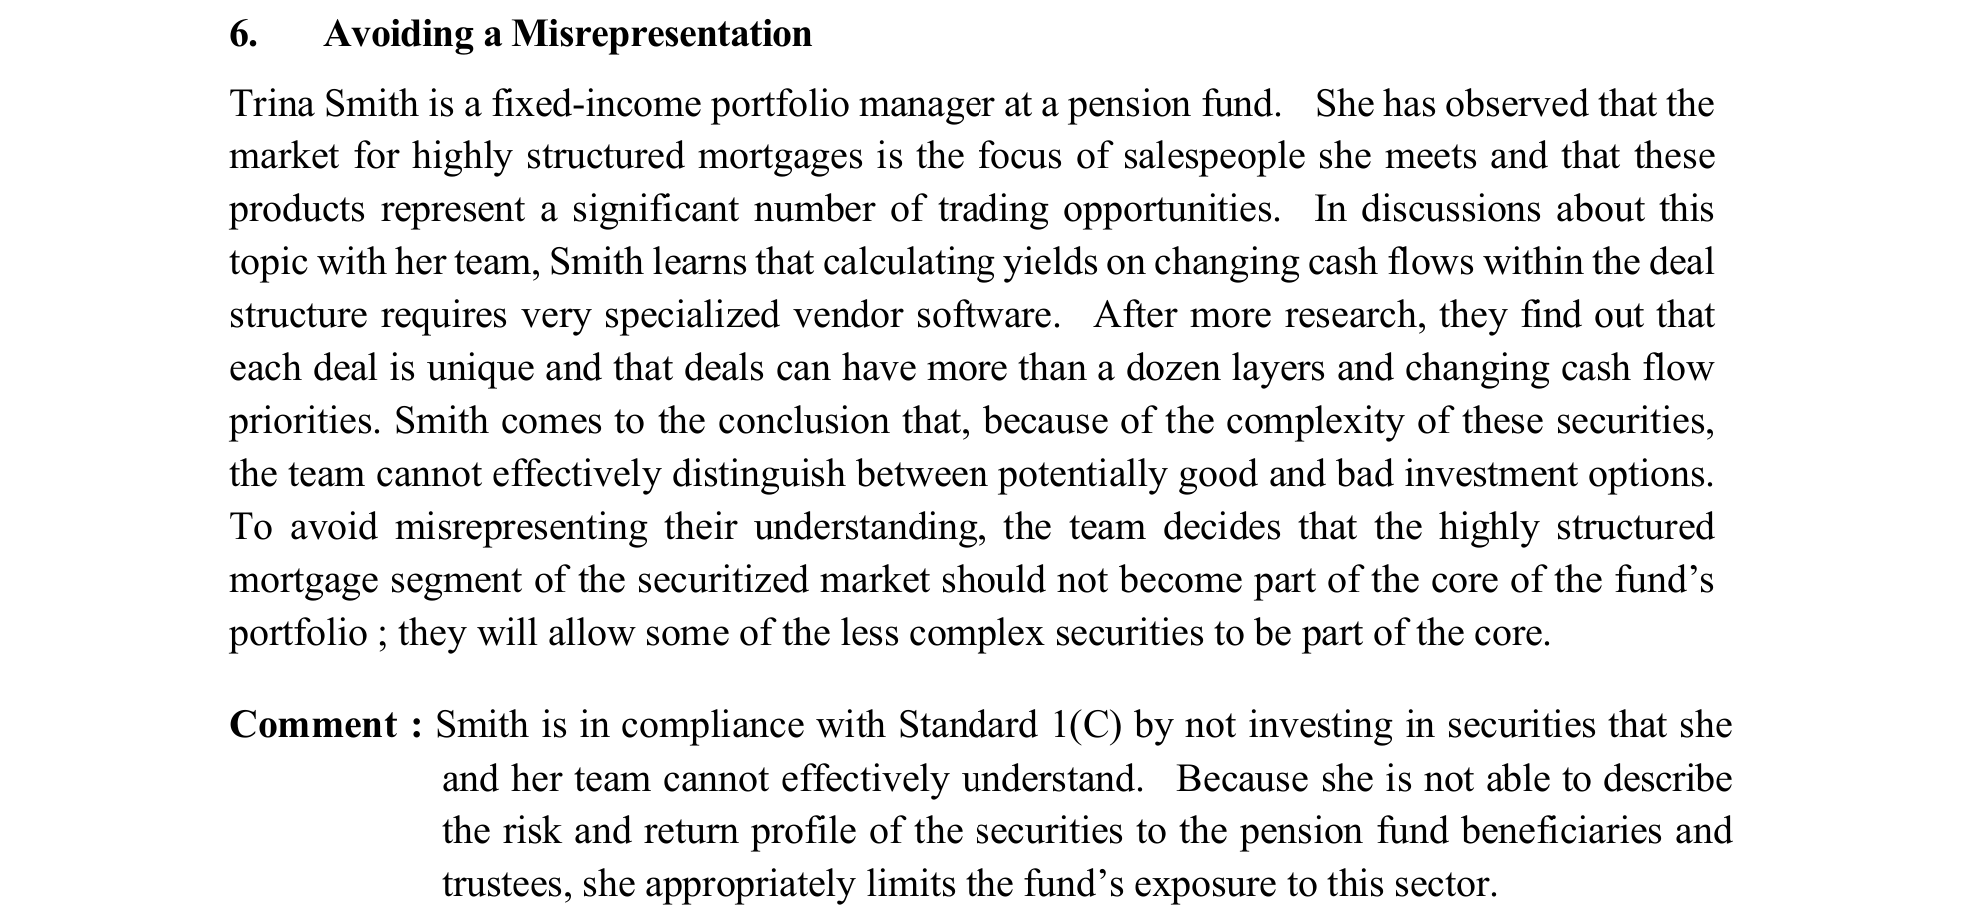
\includegraphics{image/ethic4.png}



\end{document}
